\documentclass[a4paper]{article}

%% Language and font encodings
\usepackage[english]{babel}
\usepackage[utf8x]{inputenc}
% \usepackage[T1]{fontenc}

%% Sets page size and margins
\usepackage[a4paper,top=2.5cm,bottom=2cm,left=3cm,right=3cm,marginparwidth=1.75cm]{geometry}

%% Other packages
\usepackage{amsmath}
\usepackage{graphicx}
\usepackage[colorinlistoftodos]{todonotes}
\usepackage[colorlinks=true, allcolors=blue]{hyperref}
\usepackage{apacite}
\AtBeginDocument{\urlstyle{APACsame}}
\usepackage[section]{placeins}
\usepackage{adjustbox}
\usepackage{natbib}
\usepackage{booktabs}
\addto\captionsenglish{\renewcommand*\contentsname{Table of Contents}}

% \title{\textbf{Patterns of Global and Regional Value Chain Participation in the EAC}}
\title{\textbf{Patterns of EAC Global and Regional Integration through Trade and Value Chains}}
% \author{Sebastian Krantz\footnote{Kiel Institute for the World Economy\\ \textit{Address:} Haus Welt-Club, Duesternbrooker Weg 148, D-24105 Kiel\\ \textit{E-mail:} sebastian.krantz@ifw-kiel.de}}
% \date{July 30, 2021}
\date{}

\begin{document}
\maketitle

%\vspace{1cm}

\begin{abstract}
Using detailed global trade and novel Multi-Region Input-Output (MRIO) data, %with unprecedented detail and accuracy for developing economies, 
this paper presents a rigorous examination of economic integration of the East African Community (EAC) block through trade and global value chains (GVCs). With chirurgical attention to detail, the first part of the paper expounds the key patterns and modalities of EAC members integration into regional and global trade and production networks at the aggregate, bilateral, sectoral, and bilateral-sectoral levels. The second part then provides prima facie evidence of the potential economic benefits of economic integration through trade, global, or regional value chains in the EAC at the sectoral level. The findings imply that...


% from 2005-2015, this paper empiri- 
%cally investigates the extent and patterns by which East African Community (EAC) countries have integrated into Global Value Chains (GVCs) and Regional Value Chains (RVCs). Results imply that the foreign content of exports (I2E) and the share of exports being re-exported (E2R) are between 10\% and 20\% in most EAC countries. During 2005-2015, all EAC members apart from Kenya experienced a decline in E2R. Trade in intermediates with the rest of the world remains 12-14 times greater in value-added (VA) terms than inside the EAC. Kenya expanded its role as a regional supplier of manufactured inputs (higher E2R with EAC partners), and Uganda slightly increased its agricultural input to the Kenyan % and Rwandan 
% food processing sector. Furthermore, a downstream shift is evident, by which more VA (both domestic and foreign) is used for the production of final goods while maintaining high levels of exports in primary agriculture and mining. Only Kenya was able to broadly maintain and improve its comparative advantage in manufacturing. Econometric analysis suggests that higher I2E and E2R shares increase GDP with an average elasticity of $\geq 0.25$ over 2 years. Estimates for manufacturing sectors were slightly higher at elasticities $\geq 0.3$ in response to E2R shifts. These results imply that policy measures to increase manufacturing competitiveness and promote more horizontal RVCs would benefit EAC economic growth in the medium run.  \\

\noindent \textbf{Keywords:} GVCs, EAC, regional integration, industrial development, comparative advantage\\
\textbf{JEL classification:} F14; F15; O11
\end{abstract}

% \tableofcontents
% \newpage
% \listoftables
% \listoffigures
% \newpage


\section{Introduction}

Global Value Chains (GVCs), referring to the quickly expanding internationalization of production networks, have become a central topic in trade and development policy. With the entry into force of AfCFTA in May 2019 and some progress towards its full enactment, the potential of a large common market in Africa for increased GVC-related trade, both within Africa and between Africa and the world, is of great interest to research and policy. To gauge the potential implications and distributional side-effects of AfCFTA for trade and GVCs, it is, at least to some degree, instructive to study smaller efforts of regional integration and creation of common markets in Africa, as has been the case in East Africa with the East African Community (EAC). \newline 

(Re-)founded in 2000 by Uganda, Kenya, and Tanzania as a body to facilitate regional coopera-
tion, the EAC quickly became a vehicle for economic integration. A customs union became operational in January 2005, with Kenya, the region's largest exporter, continuing to pay duties on some goods entering other countries on a declining scale until 2010 (EAC Customs Union Protocol, Article 11 and \citet{aloo2017free}). Rwanda and Burundi acceded in 2007, joining the customs union in 2009. The customs union expanded to a common market for goods, labor, and capital effective in 2010. In 2013, the Protocol for the Establishment of the EAC Monetary Union was signed, aiming for a monetary union within 10 years, subject to macro-fiscal convergence criteria. In 2016 the newly founded Republic of South Sudan joined the EAC, and the Democratic Republic of Congo joined in July 2022. Thus the EAC, particularly the years following the customs union in 2005 and the common market in 2010, provides a small case study in light of AfCFTA's broader aims. \newline 

There is, by now, a very broad academic and policy literature on the determinants and consequences of GVC integration, including for countries at different income levels. As an early example, \citet{Kummritz20162} examine patterns of GVC integration in low- and middle-income countries using the OECD TiVA database\footnote{Covering 61 countries and 34 industries for the years 1995, 2000, 2005, and 2008 to 2011.}. They find that %, apart from agriculture, developing countries are typically located more downstream in the value chain, and export more final goods. 
Low- and middle-income countries have become an integral part of GVCs and are driving their expansion, with a rising share in both the foreign content of global VA exports (9\% in 1995 to 24\% in 2011), and re-exported exports (9\% to 23\%). High-income economies use GVCs to outsource low value-added (VA) downstream production stages, but over time, many developing economies move up the value chain, and the general trend points to a more even distribution of VA across countries. \newline %South-East Asia has the highest levels of GVC integration. %, while Latin America and the Caribbean are more heterogenous with Chile and Costa Rica performing very well. 
% In Africa, Tunisia has developed backward linkages into GVCs, especially with the EU. 

The 2020 World Development Report (WDR), focusing on GVCs, classifies Africa as primarily a supplied of raw materials, with only a handful of countries (Morocco, Tunisia, Namibia, South Africa, Ethiopia, Kenya and Tanzania) engaging in limited manufacturing \citep{world2020trading}. At the same time, GDP per capita grows most rapidly when countries enter limited manufacturing GVCs. The report estimates the average benefits from a a 1 percent increase in GVC participation to boost per capita income by more than 1 percent, much more than the 0.2 percent income gain from standard trade. To enter GVCs, the report stipulates attracting FDI, improving access to finance and keeping labour costs low, as well as trade liberalization, investments in ICT and transport infrastructure, and political stability. The report constantes that African economies score low in all of these dimensions. In particular, overvalued exchange rates and restrictive labor
regulations raise the cost of labor: "manufacturing labor costs in Bangladesh are in line with its per capita income, but in many African countries, labor costs are more than twice as high." \citep{world2020trading}. \newline

These policy conclusions are broadly echoed in much early and recent work on GVCs in Africa and other developing regions. For example \citet{foster2015global} provide one of the first comprehensive analyses of GVCs in Africa, using the EORA 25 sector database over 2000-2011. They find that Africa is more involved in GVCs than many other developing regions, but mainly supplies primary goods. Downstream involvement is relatively small and shows little improvement in 1995-2011. GVC involvement also is very heterogeneous across African countries, with some relatively successful countries (Tunisia, South Africa) heavily involved in (downstream) GVCs. %At a sectoral level, \citet{foster2015global} find that manufacturing is not a major contributor to African GVC participation. 
Inner-African GVCs are also small in most African countries, with several exceptions in southern Africa. The EU is the biggest GVC partner for Africa, with increasing shares of (South-)East Asia and other transition countries. \newline

This is echoed by \citet{kowalski2015participation}\footnote{The authors conduct extensive econometric analysis using GVC indicators computed from OECD TiVA ICIOs for 57 countries in the years 1995, 2000, 2005, 2008, and 2008, WIOD ICIOs for 40 countries from 1995-2011, and EORA ICIOs for 186 countries from 1990-2011, as well as country-specific structural and policy indicators.}'s study of GVC participation in Africa, the Middle East, and Asia, which also find that that structural factors, such as geographic proximity to manufacturing hubs in Europe, North America, and East Asia, domestic market size, and the level of development, are key determinants of GVC participation.\footnote{\citet{kowalski2015participation} also note that in addition, trade and investment policy reforms (in particular low import tariffs and FDI openness), improvements in logistics and customs, intellectual property protection, infrastructure, and institutions can play a large role in promoting further engagement.} The findings are commensurate with \citet{antras2020geography}, which develop a general-equilibrium framework where trade costs imply a concentration of downstream production stages in central locations/countries (close to final demand). \citet{fernandes2022determinants} using a panel with more than 100 countries and a novel identification strategy, show that factor endowments, geography, political stability, liberal trade policies, FDI inflows, and domestic industrial capacity are key determinants of GVC participation, whereas traditional exports are less important. 
 %They state that very favorable policy environments in low-income countries can substitute to some extent for suboptimal structural factors. 
\citet{kowalski2015participation} also state that developing countries reap important benefits from GVC participation through both forward and backward linkages, including enhanced productivity, export diversification, and sophistication. Analyzing export competitiveness in different regions, they find that Asia dominates more advanced products such as electronic equipment or motor vehicles, while African and Middle Eastern regions are competitive in agriculture, food processing, and less advanced manufacturing. While all regions have become more competitive, they find little signs for a trend towards industrialization and GVC-related trade in Africa. \newline %The survival rates of export relationships in Asia are also near twice that of African export relationships. \newline  % , which they attribute to stronger regional integration and learning by doing. \newline %In terms of global integration, they find that advanced economies are becoming less important as suppliers of inputs to developing regions and that trade in intermediates is increasing both between and within the South Asia, Middle-East, and Africa regions. Finally, they find that services trade also takes on an increasing role for GVCs in various developing regions. \newline 

\citet{balie2019does} presents a careful analysis of bilateral-sectoral GVC linkages in SSA with an emphasis on food processing GVCs, and show that the trade of SSA in these chains is substantial. This is driven by a handfull of countries, including Kenya and Uganda, where the share of agriculture to total GVC participation is at 30\%, and in Kenya the food processing sector is at 15\%. They further show that bilateral trade policy is a key determinants in shaping SSA's GVC integration (both forward and backward) in the food sector, with high tariffs having a detrimental effect on GVC participation. They also confirm the results of \citet{foster2015global} that SSA GVC participation is high - at 40\%, comparable to China and India. Africa also is the continent with the highest forward integration, at 25\% of the domestic VA produced in SSA are inputs for other countries exports, and over 35\% in the case of North Africa.\newline

% GPT4 Shortened Version

%The literature on the determinants and consequences of Global Value Chain (GVC) integration is extensive, with a focus on countries at different income levels. The 2020 World Development Report (WDR) classifies Africa as primarily a supplier of raw materials, with only a few countries engaging in limited manufacturing \citep{world2020trading}. The report also highlights the importance of attracting Foreign Direct Investment (FDI), improving access to finance, keeping labour costs low, and investing in Information and Communication Technology (ICT) and transport infrastructure for GVC integration. 
%
%Several studies echo these findings. For instance, \citet{foster2015global} and \citet{kowalski2015participation} find that Africa is more involved in GVCs than many other developing regions, but mainly supplies primary goods. They also highlight the heterogeneity of GVC involvement across African countries and the importance of structural factors, such as geographic proximity to manufacturing hubs, domestic market size, and the level of development, in determining GVC participation. 
%
%\citet{Kummritz20162} and \citet{kummritz20161} examine patterns of GVC integration in low- and middle-income countries. They find that high-income economies use GVCs to outsource low value-added (VA) downstream production stages and reimport the final good. Over time, many developing economies move up the value chain, with South-East Asia showing the highest levels of GVC integration. 
%
%More recent empirical work has focused on specific aspects of GVC integration, such as domestic content in exports, GVC positioning, and the relationship of GVC and traditional trade. For example, \citet{jangam2021does} and \citet{durongkaveroj2023emphasis} show that greater participation in GVCs significantly improves domestic value-added exports and increases export performance. \citet{fernandes2022determinants} find that factor endowments, geography, political stability, liberal trade policies, FDI inflows, and domestic industrial capacity are key determinants of GVC participation. 
%
%\citet{balie2019does} presents a careful analysis of bilateral-sectoral GVC linkages in Sub-Saharan Africa (SSA) with an emphasis on food processing GVCs. They find that the trade of SSA in these chains is substantial and driven by a handful of countries. They also confirm the results of \citet{foster2015global} that SSA GVC participation is high, comparable to China and India.
%


Recent years have also seen some GVC and RVC related work on regional economic communities in Africa. Notably, \citet{obasaju2021regional} examine the impact of regional integration on upgrading through GVCs (proxied by domestic VA in exports per capita) in the EAC, Southern African Customs Union (SACU) and Economic Community of West African States (ECOWAS) in 2000-2015 using an panel-regression framework. They show that regional integration and FDI are not significant drivers of upgrading, but lagged backward GVC participation is. They do find weak positive effects of regional integration on labour productivity in the EAC and SACU (the regional communities with stronger levels of trade integration). They also show that regional hegemons in these communities (Kenya, South Africa, and Nigeria), have weak backward linkages w.r.t. other members. \citet{tinta2017determinants} studies determinants of GVC participation in ECOWAS, and finds that intra-regional trade is not a significant predictor or trade openness, but backward GVC participation is. Further, trade diversification is found to be a key predictor of backward GVC participation. \citet{engel2016sacu} provides a detailed analysis of GVC integration, position, and performance of SACU members (Botwana, Lesotho, Namibia, South Africa and Eswatini). They find that the SACU region is moderately integrated into GVCs, but the scale and nature of integration varies by country, with South Africa and Namibia most integrated. They also find that  the share of intermediates in gross trade has declined. South Africa remains a moderately important player in global trade networks and important regional hub. Lesotho shows a rapid increase in GVC integration, Namibia a moderate increase, whereas Botswana and Eswatini appear stagnant or in decline. Overall growth in GVC participation in services is stronger than in manufacturing.  South Africa is the only country with strong forward GVC integration. Lesotho, South Africa, and, to a lesser extent, Namibia, are well integrated into Backward GVCs. Examining bilateral forward and backward links shows SA's dominant role as a source of foreign content of the other members, indicating that they are more integrated into RVCs than global ones. China has grown significantly as a source of foreign content, but the EU remains the predominant partner for forward GVC participation. Overall, the GVC position is relatively upstream. 
 \newline 

%While some work has been done on RVCs in East Africa within specific industries, such as Maize value chains studied by \citet{daly2016maize}, and \citet{lwesya2022integration} provide a macroeconomic assessment, there has not yet been a detailed exposition of EAC regional integration and GVC participation using comprehensive data sources. \newline %Some landmark studies have however been conducted regarding the GVC integration of Africa and developing countries more broadly. \newline


\citet{lwesya2022integration} studies GVC integration in the EAC with respect to economic upgrading using UNCTAD-Eora GVC Panel data from 2005 to 2018. This analyis is largely complimentary to the analysis carried out in this paper. The authors compute measures of backward and forward integration and find that Kenya, Tanzania and Uganda are relatively
better integrated into GVCs, with Kenya having the deepest level of integration, expecially in terms of indirect VA and forward integration. Overall, the EAC's participation in GVCs is found to be in upstream low- and middle value-added production activities. Then, using a cross-country panel regression framework predicting domestic value added (DVA) in exports, which includes GVC indicators and other macroeconomic indicators, he finds that domestic credit, foreign direct investment, the quality of institutions and foreign value-added have significant positive effects, but observed no such effects for measures of human capital, infrastructure quality, and GDP per capita. The analysis is focused on the economic upgrading aspect, and does not provide a detailed bilateral and sector-level exposition of the regions integration into GVCs and RVCs. He also does not provide a detailed examination of how different forms of trade and GVC participation affect economic growth. The analysis also does not establish economic causality between any of the studied factors and DVA in exports. \newline

This paper adds to our understanding of GVCs and regional integration in the EAC in the following significant respects: (1) it uses better data, including gross trade flows data and the EMERGING MRIO tables, which include IO/SUT/SAM tables for 4 EAC countries; (2) it conducts a detailed examination of EAC members global and regional integration using both gross trade flows and value added content shares, paying close attention to specific bilateral linkages and sector-level patterns; (4) it constructs metrics to track regional integration in both gross and VA terms and uses them to measure progress in recent years (4) It examines the positioning of EAC members and sectors in GVCs as well as revealed comparative advantage in gross and value-added terms; (5) It analyzes the effect of conventional trade, GVC, and RCV participation on domestic value added using a bilateral-sector-level regression framework with triple fixed effects and instrumental variables for GVC participation following \citep{Kummritz20161} (weighting third-party trade costs by industry distance in the value chain). Thus it attempts to present a rigorous and detailed study of the regions global and regional integration through trade and value chains using the best available data, and to establish economic causality between different forms of trade and value-added. 

% lagged GVC indicators, and argues that this framework is better able to control for at least some of the endogeneity in GVC participation than a macro-level panel regression. \newline 


%The main aim of this paper is to map the structure of regional and international production and exports in the EAC and to produce some first evidence of the potential benefits of GVC integration for East Africa at the aggregate and sector levels. A secondary aim, more difficult to substantiate empirically, is to gauge the potential effects of regional economic integration through a customs union (2005) and common market (2010) for GVC-related trade in and with the EAC. The analysis follows the seminal works of \citet{hummels2001nature}, \citet{koopman2014tracing}, \citet{wang2013quantifying}, as well as \citet{Kummritz20161} and \citet{Kummritz20162}\footnote{More sophisticated GVC decompositions or econometric approaches are considered infeasible in light of the low quality of the EORA ICIO tables for developing countries.}. \newline 

\newpage

\section{Data}

Most GVC analysis uses Inter-Country Input-Output tables (ICIOs), such as those published by the OECD (TiVA) or the World Input-Output Database (WIOD)  \citep{timmer2012world}. These tables state supply and demand relationships in gross terms between industries within and across countries \citep{Kummritz2014}. The WIOD and TiVA databases however focus on OECD countries, with very limited coverage of Sub-Saharan Africa (SSA). This paper, therefore, uses two Multi-Region Input-Output (MRIO) databases that are global in scope. \newline % and developed with environmental science applications in mind. \newline 

 The first is the EORA 26 Global MRIO \citep{lenzen2012mapping, lenzen2013building}, which has extensive coverage of 189 countries and 26 sectors from 1990-2015, and uses 74 country IOT/SUTs and detailed international macroeconomic and trade data as input. EORA relies on sophisticated supercomputing methods to impute and harmonize data across countries and is therefore considered less reliable than the OECD or WIOD tables, particularly for small countries like EAC members the data can be highly distorted. The Kenya 2010 IOT is the only source of EAC national data used in EORA \citep{lenzen2013building}. In 2021 an update of EORA was released, adding administrative data through 2018 and WEO-based forecasts through 2021. This release introduced a very large structural break into the time series in 2016, resulting in different macroeconomic totals and GVC indicators for EAC members. % (particularly visible for small countries like EAC members, see Appendix E). 
This most recent release is also not free but must be purchased. Due to the structural break and the non-open nature of the data, I focus the analysis on the initial EORA release through 2015. Since GVCs are a recent phenomenon, particularly in Africa, and the EAC customs union only became operational in 2005, I consider the EORA 26 tables from 2000 onwards. Data from 1990 shows no interesting trends in GVC engagement and is also devoid of IO input data for EAC countries. %Appendix E shows the results computed on the extended 1990-2021 database. 
EORA is denominated in thousands of current USD at basic prices\footnote{The basic price is the amount receivable by the producer from the purchaser for a unit of a good or service produced, as output minus any tax payable, and plus any subsidy receivable. It excludes any transport charges invoiced separately by the producer.}. % The data are scaled to be consistent with global aggregates, but may heavily distort data for smaller countries. 
Appendix D shows GDP and gross exports computed for the World and the EAC countries, including, in Figure \ref{fig:EORADQMT}, official EORA data quality reports for macroeconomic totals\footnote{While global GDP is broadly consistent with representative estimates, the GDP of EAC countries is highly distorted. Most notably, the GDP of Tanzania has been decreasing. The situation is better for exports, whose level and sectoral composition is roughly consistent with estimates from other sources. Thus detailed analysis and results from EORA should be treated with great caution, particularly for Tanzania.}. %, as the data analyzed was not constructed to accurately reflect macroeconomic totals in developing countries. 
% Nevertheless, EORA is the only global ICIO database currently in existence and may be used to get a rough idea about GVCs and RVCs in the EAC. Most findings of this paper appear plausible in light of observable production and trading patterns, but should not be over-interpreted. 
Despite its shortcomings, EORA has been used in much research on GVCs in Africa, including the 2020 World Development Report (WDR) \citep{world2020trading}.\newline 
% The EORA database comes in a full version with heterogenous sector disaggregations %as provided by country Supply and Use Tables 
% and an aggregated 26-sector version that is harmonized across countries. I consider EORA 26, of which data until 2015 is available at the time of conducting this research\footnote{In 2021 an update of EORA was released, adding administrative data through 2018 and WEO-based forecasts through 2021 (which must be purchased). The revision however introduced a very large structural break into the time series in 2016, resulting in different macroeconomic totals and GVC indicators. It is not possible to obtain a complete revised series. Since this research is more concerned with the early years of EAC integration following the customs union in 2005 and common market in 2010, and with trends in GVC indicators, I decided to stick with the first edition of the EORA database with data through 2015. Appendix E shows some GVC indicators computed on the combined database and discusses some implications of the structural break in the data.}. 

Due to the shortcomings of EORA in terms of accuracy and usage of national data for developing countries, I also use the more recently introduced EMERGING (EM) MRIO tables \citep{huo2022full}. This impressive effort creates a global MRIO database covering 245 countries and territories in 135 sectors, for the years 2015-2019. A recent update (v2) also provides a table for 2010. EMERGING uses 111 national IO/SUT/SAM tables, alongside detailed trade and macroeconomic data. In particular, the UN Comtrade database is utilized to the fullest extent to provide greater sectoral detail than EORA. Macroeconomic data from national statistical offices is used where available and reconciled (scaled) using World Bank Data. The purpose of the MRIO is to provide greater detail and accuracy for emerging economies than EORA, and the construction process reflects this. From EAC countries, EM uses a SAM and sectoral GDP from Uganda up to 2016, and the same information up to 2019 for Rwanda and Kenya. For Tanzania, EM uses a SAM and an IO table up to 2017. For Burundi, Congo (DRC) and South Sudan only international data (Comtrade and macro data) is available. Thus EM incorporates, to the extent possible, national data from these EAC countries in a harmonized global MRIO framework. EM is denominated in millions of current USD at basic prices. \newline

The WDR 2020 \citep{world2020trading} also provides GVC indicators from EORA 2015, and \citet{mancini2023positioning} provide GVC positioning indicators using the same database following \citet{fally2012production}, \citet{antras2012measuring} and \citet{antras2013organizing, antras2018measurement}. These precomputed indicators are used to verify manually computed indicators. This is important, because I aggregate the non-EAC World and/or sectoral resolution for different indicators to lift computational constraints\footnote{In particular, EMERGING has 245 countries/territories and 134 sectors, implying 32,830 rows and columns or 1 billion records in the transaction matrix. It is computationally infeasible for me to compute GVC indicators directly on these tables, and also the full EORA database (186 x 26 = 4836 rows and columns observed over 21 years) strains my computing resources for non-trivial GVC indicators.} and facilitate interpretation. In particular,
% computed using a more sophisticated source-based decomposition of \citet{borin2019measuring} at the country-sector level which is used as a check on the manually computed GVC indicators presented in this paper. This paper uses simpler methods based on \citep{hummels2001nature}, \citet{koopman2014tracing} and \citet{wang2013quantifying} to compute GVC indicators, which were shown to have some biases in accounting double counted items (see \citet{borin2019measuring}), but are conceptually simpler and, importantly, much easier to obtain in large quantity and bilateral $+$ sectoral detail using the open source implementation in the R package \emph{decompr} \citep{Kummritz2014}. Biases from these methods are very small in the study context at hand because double counted items - resulting from two-way processing trade, are not a salient component in the exports of these developing countries. \newline 
to enhance the interpretation of results while preserving some level of detail, the non-EAC world is aggregated into 11 geographic and trade regions summarised in Table \ref{tab:ctry}, and, in more detail, in Table \ref{tab:ctrydet}. This reduces the size of the transaction tables considerably. % Reducing the number of countries while maintaining full sectoral detail results in identical GVC indicators for EAC members - verified using WDR 2020 data. %from $189 \times 26 = 4914$ rows and columns to $(6 + 11)\times 26 = 442$ rows and columns. \newline

\begin{table}[h!]
\centering
\caption{\textsc{Regional Aggregation}}

\label{tab:ctry}
\vspace{2mm}
\begin{tabular}{llrr} \toprule
& & \multicolumn{2}{c}{\textit{Countries \& Territories}} \\
\textit{Region} & \textit{Description} & EORA & EMERGING \\ \midrule
EAC & East African Community & 7 & 7 \\
SSA & Sub-Saharan Africa (Excluding EAC) & 38 & 41 \\
EUU & European Union + UK & 28 & 29 \\
ECA & Europe and Central Asia (Non-EU) & 26 & 29 \\
MEA & Middle East and North Africa & 20 & 21\\
NAC & North America and Canada & 3 & 13 \\
LAC & Latin America and Carribean & 32 & 44 \\
ASE & ASEAN & 10 & 10 \\
SAS & South Asia & 8 & 9 \\
CHN & China & 3 & 3 \\
ROA & Rest of Asia & 7 & 14 \\
OCE & Oceania & 6 & 22 \\ \midrule
SUM: & 7 EAC Members + 11 World Regions & 188 & 245
 \\ \bottomrule
\end{tabular}
\end{table}
\FloatBarrier

% \newpage

To verify EM, \citep{huo2022full} develop a broad sector classification of 17 sectors and mappings from the sectors of major global ICIOs (EXIOBASE3rx, OECD-TiVA, EORA, GTAP, and EM) to these broad sectors. I use these mappings to report results at the sector level. Most GVC indicators are computed at the full sector resolution using STATA's ICIO package \citep{belotti2020icio} and the default source-based exporter perspective \citep{borin2019measuring} also used in the WDR, which permits aggregation of GVC indicators across sectors. Table \ref{tab:sec} shows the 26 EORA sectors\footnote{Sector codes are assigned and used throughout the paper, but are not found in the EORA 26 database.} and their mapping to broad sectors. Appendix Table \ref{tab:EMSec} shows the mapping for EM. 
 
 
\begin{table}[h!]
\centering
\caption{\textsc{EORA 26 Sectors and Mapping to Broad Sectors}}
\label{tab:sec}
\vspace{2mm}
\resizebox{\textwidth}{!}{
\begin{tabular}{llll}
  \toprule
Code & EORA 26 Sector Definition & BSC & Broad Sector Definition of \citet{huo2022full} \\ 
  \midrule
AGR & Agriculture & AFF & Agriculture, Hunting, Forestry \& Fishing \\ 
  FIS & Fishing & AFF & Agriculture, Hunting, Forestry \& Fishing \\ 
  MIN & Mining and Quarrying & MIN & Mining \& Quarrying \\ 
  FBE & Food \& Beverages & FBE & Food Production, Beverages \& Tobacco \\ 
  TEX & Textiles and Wearing Apparel & TEX & Textiles, Leather \& Wearing Apparel \\ 
  WAP & Wood and Paper & WAP & Wood, Paper \& Publishing \\ 
  PCM & Petroleum, Chemical and Non-Metallic Mineral Products & PCM & Petroleum, Chemicals \& Non-Metallic Mineral Products \\ 
  MPR & Metal Products & MPR & Metal \& Metal Products \\ 
  ELM & Electrical and Machinery & ELM & Electrical \& Machinery \\ 
  TEQ & Transport Equipment & TEQ & Transport Equipment \\ 
  MAN & Other Manufacturing & MAN & Manufacturing \& Recycling \\ 
  REC & Recycling & MAN & Manufacturing \& Recycling \\ 
  EGW & Electricity, Gas and Water & EGW & Electricity, Gas \& Water \\ 
  CON & Construction & CON & Construction \\ 
  MRE & Maintenance and Repair & SMH & Sale, Maintenance \& Repair of Vehicles; Fuel; Trade; Hotels \& Restaurants \\ 
  WTR & Wholesale Trade & SMH & Sale, Maintenance \& Repair of Vehicles; Fuel; Trade; Hotels \& Restaurants \\ 
  RTR & Retail Trade & SMH & Sale, Maintenance \& Repair of Vehicles; Fuel; Trade; Hotels \& Restaurants \\ 
  AFS & Hotels and Restraurants & SMH & Sale, Maintenance \& Repair of Vehicles; Fuel; Trade; Hotels \& Restaurants \\ 
  TRA & Transport & TRA & Transport \\ 
  PTE & Post and Telecommunications & PTE & Post \& Telecommunications \\ 
  FIB & Finacial Intermediation and Business Activities & FIB & Financial Intermediation \& Business Activity \\ 
  PAD & Public Administration & PAO & Public Administration; Education; Health; Recreation; Other Services \\ 
  EHO & Education, Health and Other Services & PAO & Public Administration; Education; Health; Recreation; Other Services \\ 
  PHH & Private Households & PAO & Public Administration; Education; Health; Recreation; Other Services \\ 
  OTH & Others & PAO & Public Administration; Education; Health; Recreation; Other Services \\ 
  REI & Re-Export \& Re-Import & PAO & Public Administration; Education; Health; Recreation; Other Services \\ 
   \bottomrule
\end{tabular}
}
\end{table}
\FloatBarrier

Finally, this study also uses gross trade flows data from the using CEPII's BACI \citep{CEPIIBACI} (HS 1996 version) and the IMF's Direction of Trade Statistics (DOTS) \citep{IMFDOTS} databases. EM's goods producing sectors are identical to the 2-Digit HS codes, so  that BACI can be aggregated to match the MRIO databases using the mapping in Table \ref{tab:EMSec}. The DOTS database records aggregate bilateral trade, where imports are denominated in Const Insurance Freight (CIF) terms, i.e., including trade and insurance costs. 


\newpage


\section{Gross Flows}

In light of the known macroeconomic inconsistencies in EORA for EAC countries, and that VA flows are estimated from gross flows, this section examines EAC trade integration in gross terms using BACI, DOTS, and gross total and intermediate flows recorded in the EORA and EM MRIO tables. \newline

Figure \ref{fig:MIG} shows migration flow diagrams of EAC trade flows averaged between 2010 and 2019. All databases emphasize Kenya as the regional trading hegemon, followed by Uganda and Tanzania, but EORA gives disproportional weight to Kenya and shrinks the other countries, whereas EM overemphasizes Rwanda and Uganda a bit and also shrinks Congo. It is particularly notable that the large exports from Congo to Tanzania are not reflected in either EORA or EM. An examination of BACI reveals that 88\% of this 550 million USD flow is copper, and 7.4\% precious metals. The DRC does not trade with other EAC members to a similar extent. The bottom half of Figure \ref{fig:MIG} includes the rest of the world (ROW) as a trading partner. 

% \todo[inline]{Compute Migration Diagrams on 2010-2020 data?? using average/median annual shares??}

\begin{figure}[h!] \vspace{-1mm}
\centering
\caption{\label{fig:MIG}\textsc{Average Gross Trade Flows from 2010-2019: 4 Databases: USD Billions}}
\vspace{2mm}
%\begin{adjustbox}{center}
\resizebox{\textwidth}{!}{
\begin{tabular}{cccc}
CEPII BACI & IMF DOTS & EORA (Basic Prices) & EMERGING (Basic Prices) \\
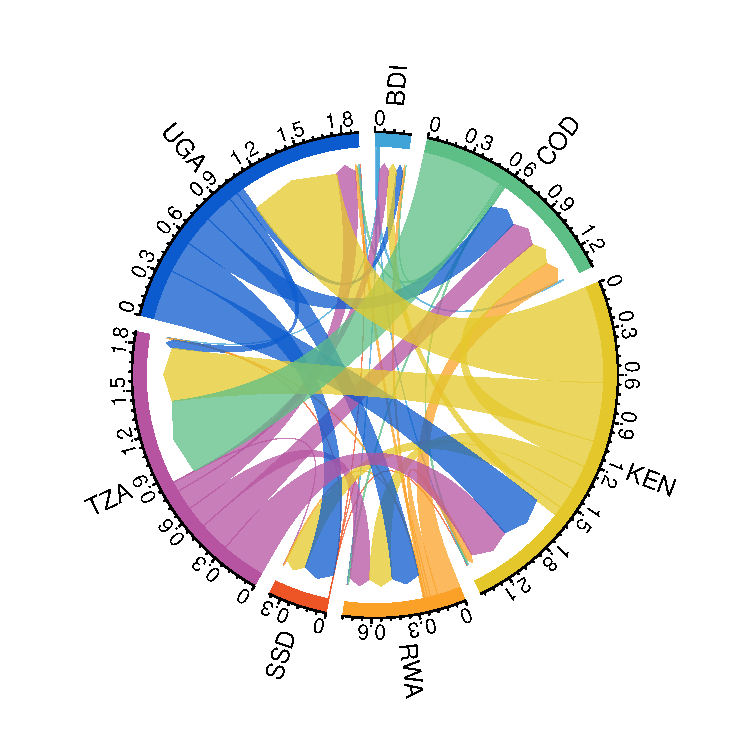
\includegraphics[width=0.4\textwidth, trim= {1.3cm 0.8cm 1.1cm 1cm}, clip]{"../Figures/REV/BACI_MIG_2010_19.pdf"} & %trim={<left> <lower> <right> <upper>}
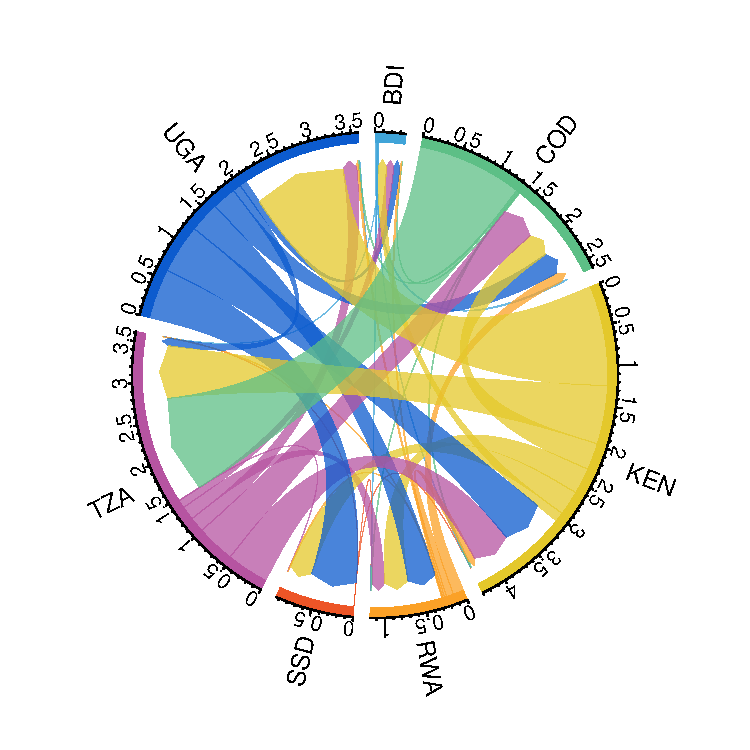
\includegraphics[width=0.4\textwidth, trim= {1.3cm 0.8cm 1.1cm 1cm}, clip]{"../Figures/REV/DOT_MIG_2010_19.pdf"} &
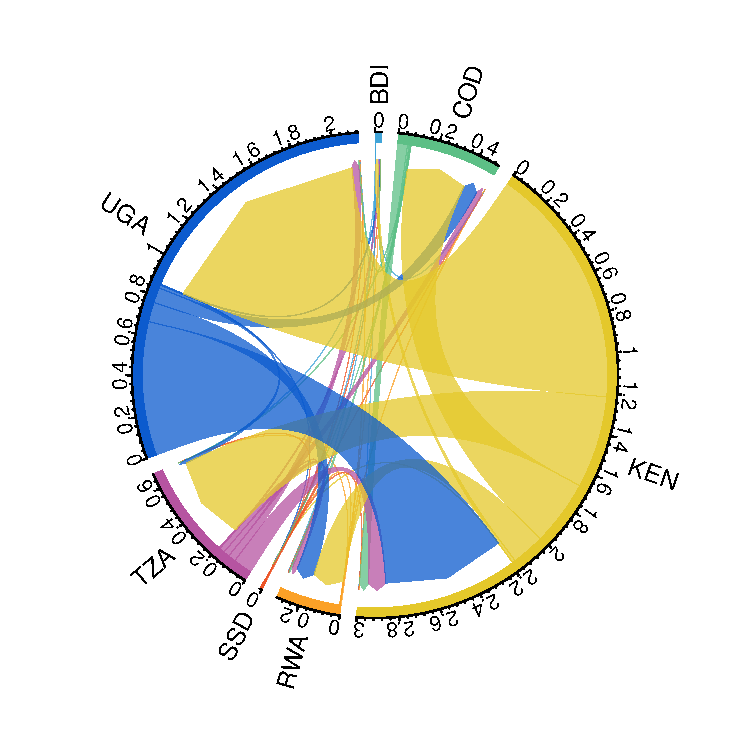
\includegraphics[width=0.4\textwidth, trim= {1.3cm 0.8cm 1.1cm 1cm}, clip]{"../Figures/REV/EORA_MIG_2010_19.pdf"} & 
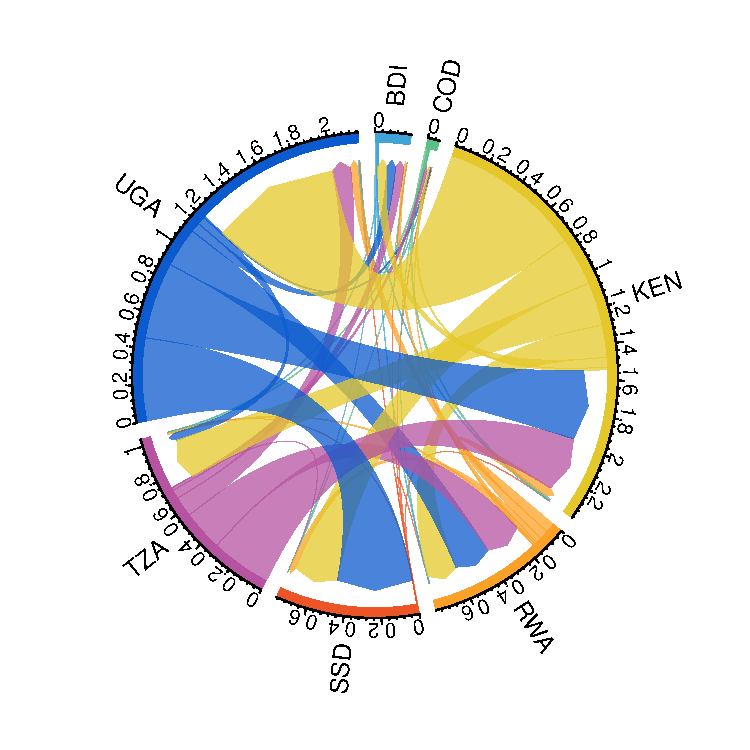
\includegraphics[width=0.4\textwidth, trim= {1.3cm 0.8cm 1.1cm 1cm}, clip]{"../Figures/REV/EM_MIG_2010_19.pdf"} \\
% CEPII BACI & IMF DOTS& EORA (Basic Prices) \\
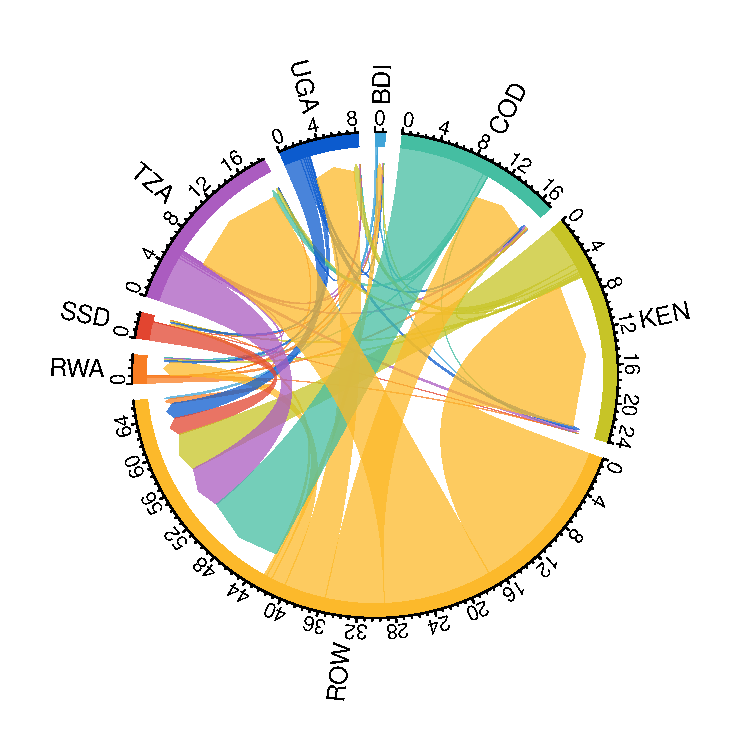
\includegraphics[width=0.4\textwidth, trim= {0.85cm 0.8cm 1cm 1cm}, clip]{"../Figures/REV/BACI_MIG_2010_19_ROW.pdf"} & %trim={<left> <lower> <right> <upper>}
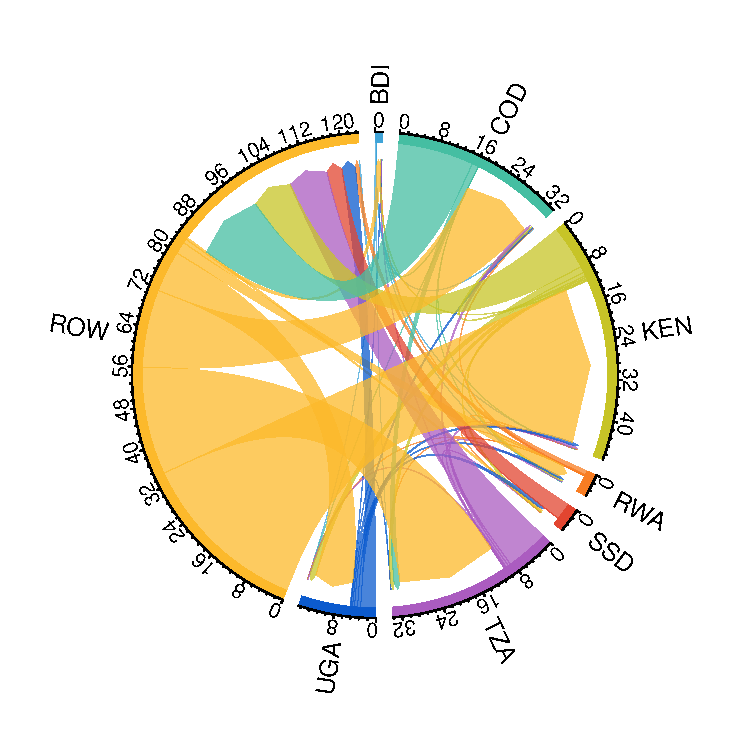
\includegraphics[width=0.4\textwidth, trim= {0.8cm 0.8cm 1cm 1cm}, clip]{"../Figures/REV/DOT_MIG_2010_19_ROW.pdf"} &
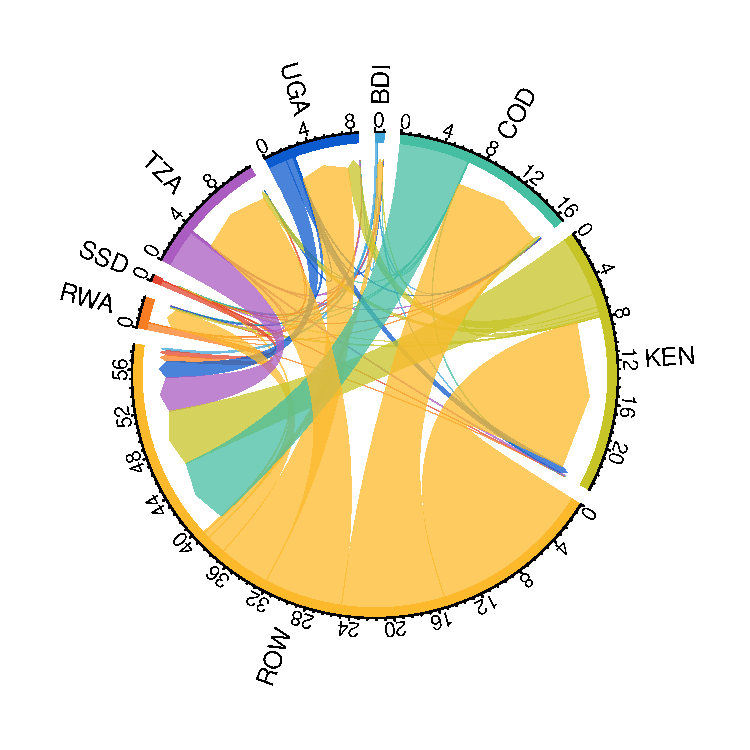
\includegraphics[width=0.4\textwidth, trim= {1cm 0.8cm 0.9cm 1cm}, clip]{"../Figures/REV/EORA_MIG_2010_19_ROW.pdf"} &
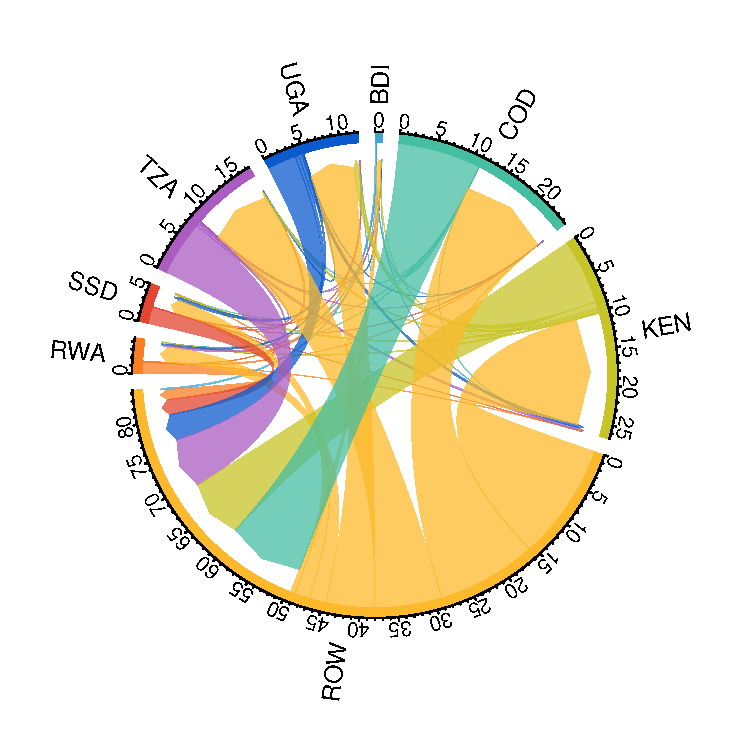
\includegraphics[width=0.4\textwidth, trim= {0.8cm 0.8cm 1cm 1cm}, clip]{"../Figures/REV/EM_MIG_2010_19_ROW.pdf"}
\end{tabular}
}
\raggedright
\scriptsize 
\emph{Notes:} Figure shows the mean of bilateral gross trade flows over years 2010-19 recorded in billions of current USD. The top panel shows inner-EAC flows, the bottom panel includes rest of the world (ROW) as a trading partner. The circular axis records the total flows (exports + imports) for each partner. Produced using the \emph{migest} R package \citep{rmigest}.
\end{figure}
\FloatBarrier

In all databases, trade with ROW dominates inner-EAC trade. To quantify these diagrams: according to BACI, inner EAC trade is 15 times smaller than EAC trade with ROW, in DOTS 14.9 times, EORA 17.5 times, and EM 22.9 times smaller. When excluding South Sudan and Congo which only joined recently (2016 and 2022), the ratios increase to 18.6 (BACI), 19.5 (DOTS), 14.9 (EORA (decrease)), and 19.7 (EM). Figure \ref{fig:EAC_ROW_Ratios} shows the evolution of this ratio for the 5 early EAC members since 2007 (EAC5), smoothed using a backward looking 5-year moving average. 

\begin{figure}[h!] \vspace{-1mm}
\centering
\caption{\label{fig:EAC_ROW_Ratios} \textsc{Gross ROW-EAC5 Trade to Inner EAC5 Trade Ratio}}
\vspace{2mm}
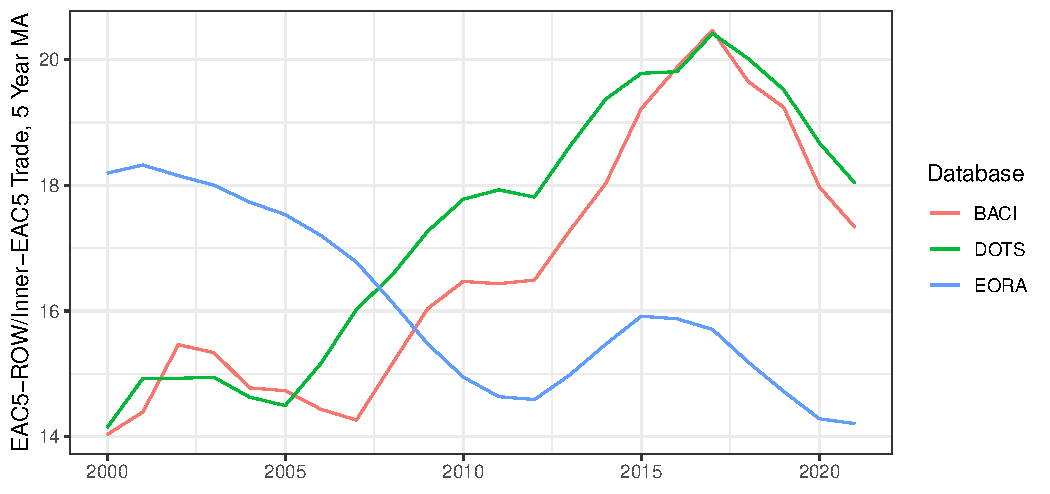
\includegraphics[width = 0.8\textwidth]{"../Figures/REV/ROW_EAC5_Trade_Ratios_5YMA.pdf"} \\
\raggedright
\scriptsize 
\emph{Notes:} Figure shows the ratio of EAC5 $\Leftrightarrow$ ROW to inner-EAC5 trade (exports + imports), smoothed using a backward looking 5-year moving average. The EAC5 includes Tanzania, Kenya, Uganda, Rwanda and Burundi.
\vspace{-10mm}
\end{figure}
\FloatBarrier

Figure \ref{fig:EAC_ROW_Ratios} indicates that up to 2017, there has been a relative disintegration of the EAC5 in terms of gross trade. However, in 2018 and 2019 trade with ROW slowed a bit, and in 2020 the COVID shock also strengthened regional trade again. %\todo{How to obtain the same ratios to the diagrams}. 
This can be disaggregated further by exports and imports, also considering individual members EAC trade shares. \newline 

Figure \ref{fig:GTEACshares} shows the EAC5 share in members and total EAC5 exports and imports, i.e., the inverse of the ratio in Figure \ref{fig:EAC_ROW_Ratios} at a more disaggregated level. Over the period, Uganda substantially increased the share of its exports destined to EAC5 partners, reaching 28\% in 2016 and falling again in recent years. Tanzania also increased its EAC5 export share from about 7\% in 2000 to 15\% in 2021. Kenya on the other hand descreased its EAC export share from 25\% in 2000 to 20\% in 2021. Rwanda shows a declining tend in both export and import share since 2012. In Burundi the EAC5 share is constant since 2005. The total EAC5 (black line) shows a slight decline from 2010 (18\%) to 2020 (16\%). On the import side there is a clear decline in the EAC5 share from 10\% in 2000 to 7.5\% in 2020. This is also mainly driven by Uganda and Tanzania. Kenya therewhile increased its EAC5 import share from 1\% in 2000 to 4\% in 2020. This pattern is in line with \citet{obasaju2021regional}'s observation that the regional hegemon (Kenya) has weak backward linkages (imports) with other REC members, but strong forward linkages (exports) - as documented, in the case of South Africa's role in SACU, by \citet{engel2016sacu}. Figure \ref{fig:GTEACshares} shows that in the EAC5 this pattern has weakened slightly, but integration in gross trade has not improved in overall terms. 

\begin{figure}[h!] %\vspace{-3mm}
\centering
\caption{\label{fig:GTEACshares}\textsc{EAC5 Share in Members Gross Trade Flows}}
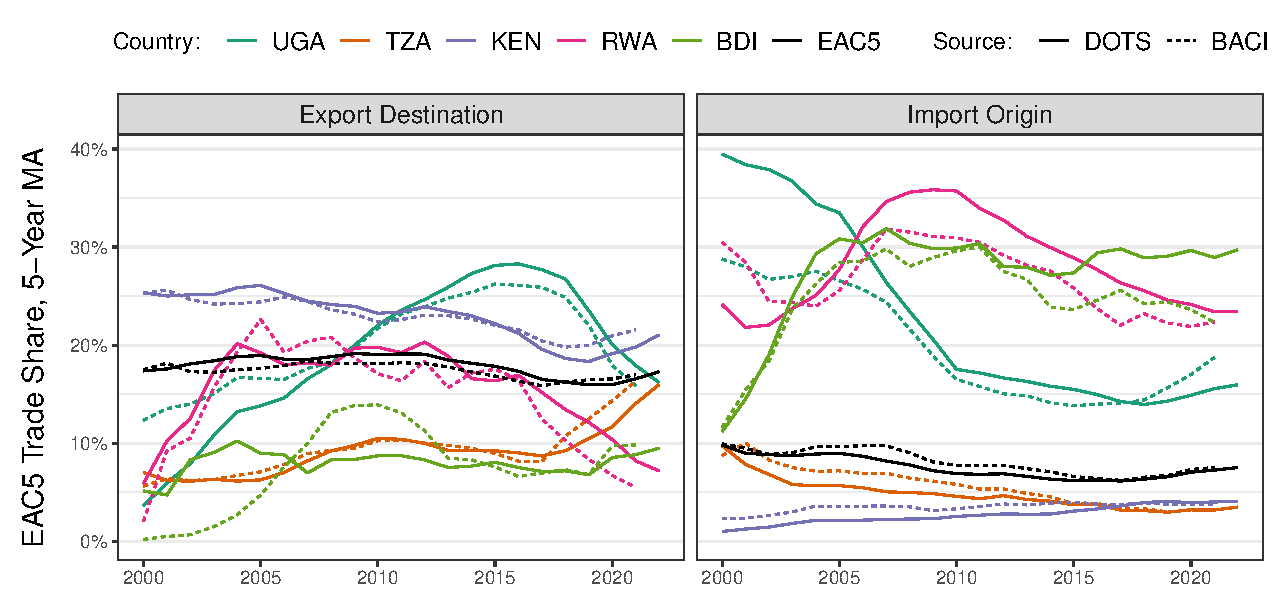
\includegraphics[width=0.9\textwidth, trim= {0 0 0 0}, clip]{"../Figures/REV/GT_EAC5_shares_ts.pdf"} \\ % "../Figures/VA_EAC_shares_ts".pdf
\raggedright
\scriptsize 
\emph{Notes:} Figure shows the EAC5 share in members total exports and imports, smoothed using a backward looking 5-year moving average. The black line also shows the EAC5's total share of exports and imports with itself.
\end{figure}
\FloatBarrier


When dividing trade flows broadly into agricultural products, processed foods and beverages, and manufactured goods\footnote{Services trade is available in the MRIO tables but not in BACI}, some further heterogeneity emerges. Figure \ref{fig:MIG_SEC_BACI} shows these flows using the BACI database, Appendix Figures \ref{fig:MIG_SEC_EORA} and \ref{fig:MIG_SEC_EM} using EORA and EM, respectively. \newline 

According to all databases, Uganda and Tanzania are large suppliers of agricultural produce in the EAC. All countries have some stakes in processed foods and beverages, with Uganda supplying the most, followed by Kenya. In manufacturing, Kenya has a distinct lead, followed by Tanzania and Uganda. With ROW, all EAC countries are large agricultural exporters and importers of manufactured products. Kenya is the largest EAC supplier of both agriculture and processed foods to ROW, whereas it only plays a minor supplier role in the EAC. Tanzania supplies large amounts of gold, and Congo large amounts of minerals to ROW, which are subsumed under MPR and PCM in Table \ref{tab:sec}, making Kenya also the largest EAC exporter of manufactures. The data thus expound differences in the nature of trade both within the EAC and with ROW. Shared capacities exists for foods and beverages production, which has also been the focus of policy makers and regional studies, such as \citet{Daly2017RVCs} which show that while Uganda exports diary and maize produce to Kenya for processing, it has also received FDI and begun to upgrade its own food processing sector. The Ugandan Ministry of Finance and Planning and IGC Uganda \citep{EGF21, fowler2019agro} and IFPRI \citep{van2020institutional} have identified agro-industrialization as an important pillar of growth and transformation for the country. 

\begin{figure}[h!] \vspace{-1mm}
\centering
\caption{\label{fig:MIG_SEC_BACI}\textsc{Average 2010-2019 BACI Trade Flows by Broad Sector: USD Billions}}
\vspace{2mm}
\resizebox{\textwidth}{!}{
\begin{tabular}{ccc}
Agriculture \& Livestock & Foods \& Beverages & Manufactured Goods \\
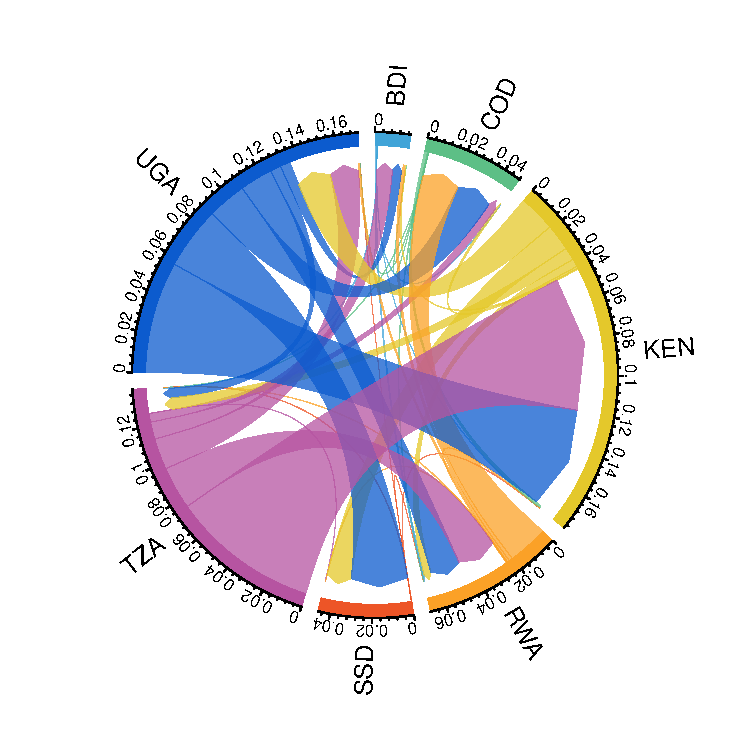
\includegraphics[width=0.4\textwidth, trim= {1.3cm 0.8cm 0.95cm 1cm}, clip]{"../Figures/REV/BACI_MIG_AGR_2010_19.pdf"} & %trim={<left> <lower> <right> <upper>}
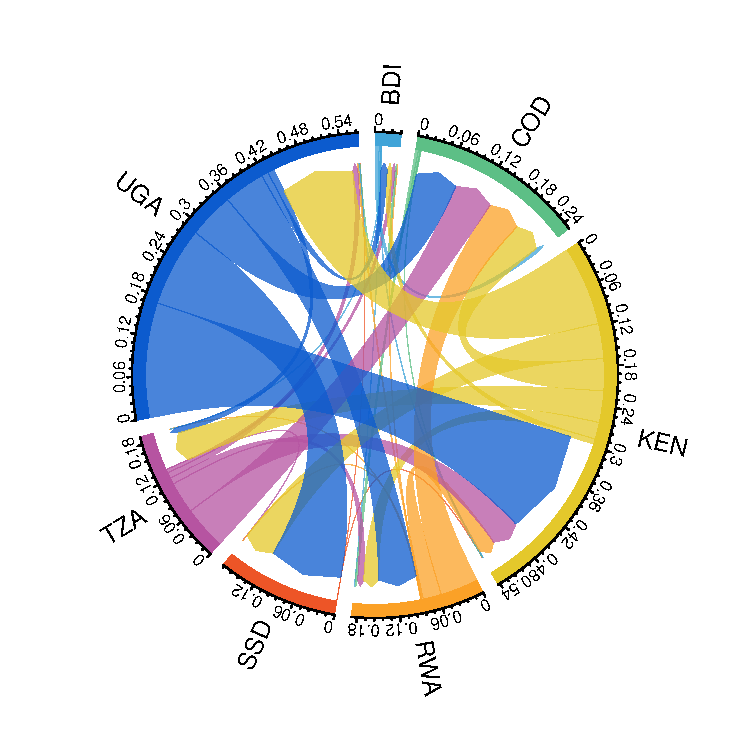
\includegraphics[width=0.4\textwidth, trim= {1.3cm 0.8cm 1cm 1cm}, clip]{"../Figures/REV/BACI_MIG_FBE_2010_19.pdf"} &
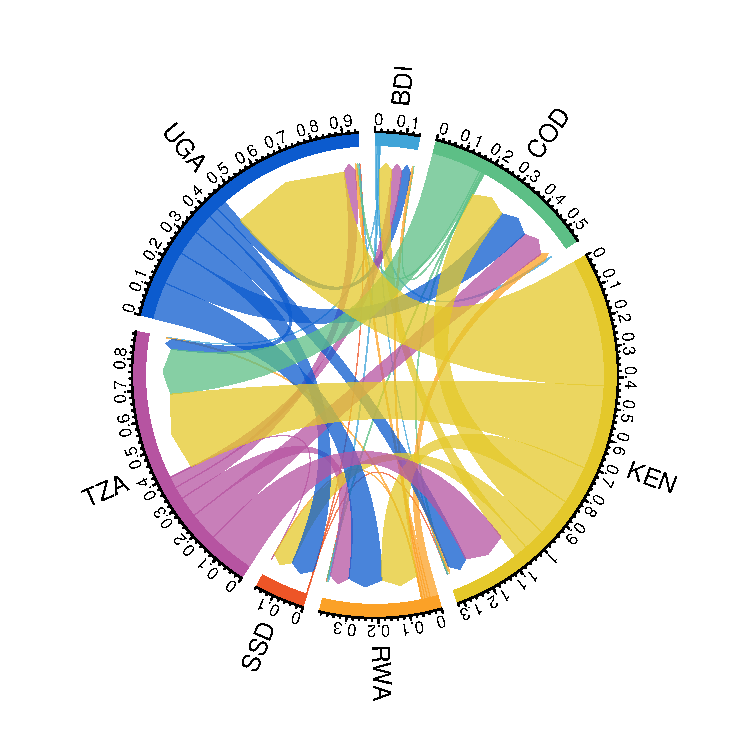
\includegraphics[width=0.4\textwidth, trim= {1.3cm 0.8cm 1.1cm 1cm}, clip]{"../Figures/REV/BACI_MIG_MAN_2010_19.pdf"} \\
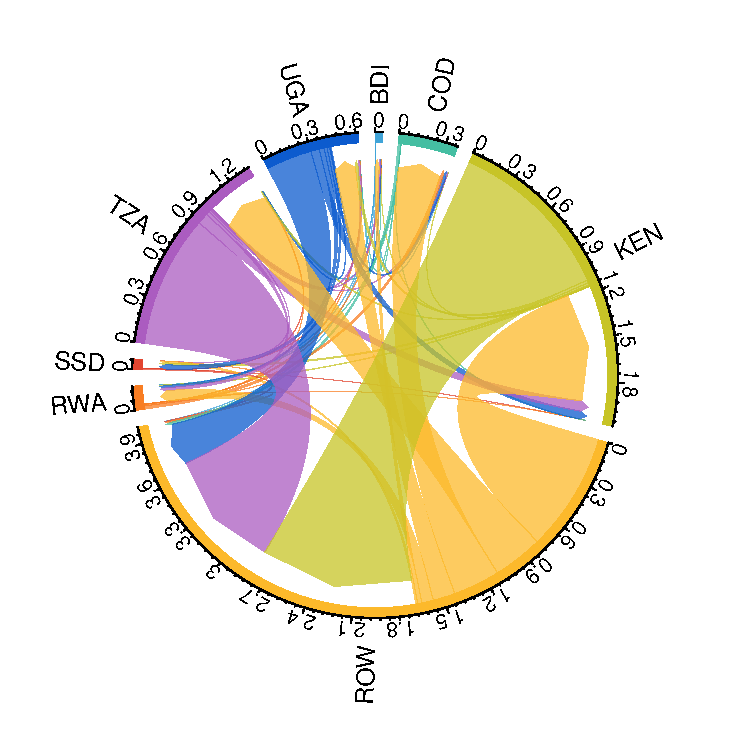
\includegraphics[width=0.4\textwidth, trim= {0.85cm 0.8cm 1.1cm 1cm}, clip]{"../Figures/REV/BACI_MIG_AGR_2010_19_ROW.pdf"} & %trim={<left> <lower> <right> <upper>}
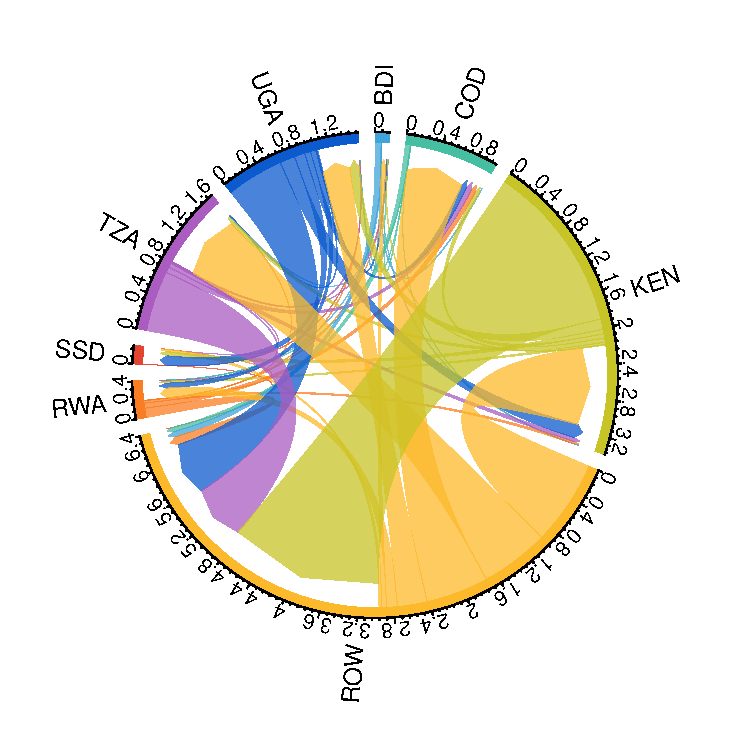
\includegraphics[width=0.4\textwidth, trim= {0.85cm 0.8cm 1.1cm 1cm}, clip]{"../Figures/REV/BACI_MIG_FBE_2010_19_ROW.pdf"} &
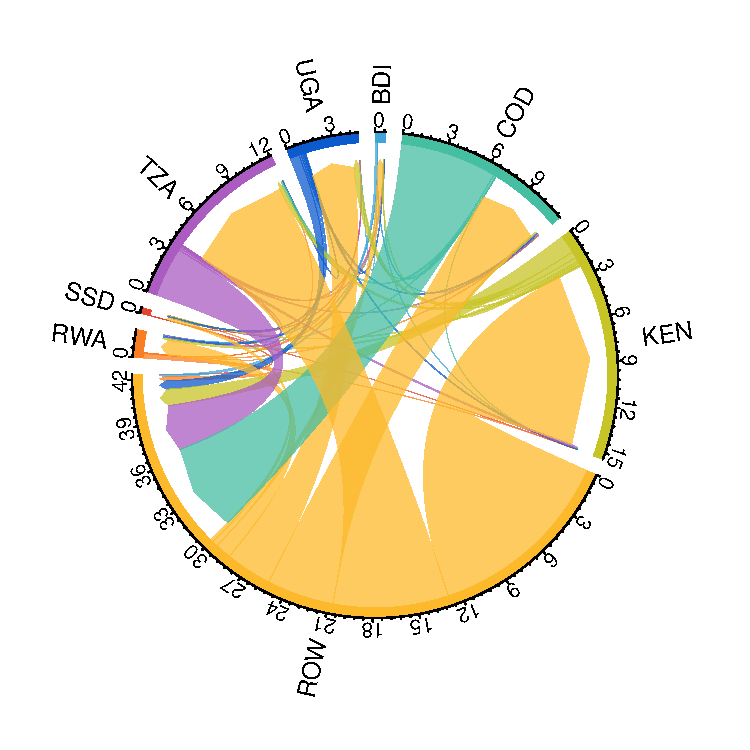
\includegraphics[width=0.4\textwidth, trim= {0.85cm 0.8cm 1cm 1cm}, clip]{"../Figures/REV/BACI_MIG_MAN_2010_19_ROW.pdf"} \\
\end{tabular}
}
\raggedright
\scriptsize 
\emph{Notes:} Figure shows the mean of bilateral gross trade flows over years 2010-19 recorded in billions of current USD according to CEPII BACI. The top panel shows inner-EAC flows, the bottom panel includes rest of the world (ROW) as a trading partner. The circular axis records the total flows (exports + imports) for each partner. The broad sectors shown are AFF (left), FBE (middle) and TEX-MAN (right) in Table \ref{tab:sec}. Produced using the \emph{migest} R package \citep{rmigest}.
\end{figure}
\FloatBarrier

Figure \ref{fig:EAC_ROW_Ratios_Sec} shows corresponding ratios of EAC5-ROW to inner-EAC5 trade, indicating that agriculture and, to a lesser extent, foods and beverages assume increasing shares of overall EAC trade in these sectors. According to BACI, in 2020, the inner-EAC5 trade in agricultural products was 10 times smaller than EAC-ROW trade, down from almost 40 times smaller in 2000. Similarly, foods \& beverages inner-EAC5 trade was 11 times smaller in 2020, compared to 16 times smaller in 2000. In constrast, the ratio in manufactures shows an oscillating increase to 20 in 2020, up from 15 in 2000. These developments are also reflected in the MRIO databases. 

\begin{figure}[h!]
\centering
\caption{\label{fig:EAC_ROW_Ratios_Sec} Gross ROW-EAC5 Trade to Inner EAC5 Trade Ratio by Broad Sector}
% \vspace{2mm}
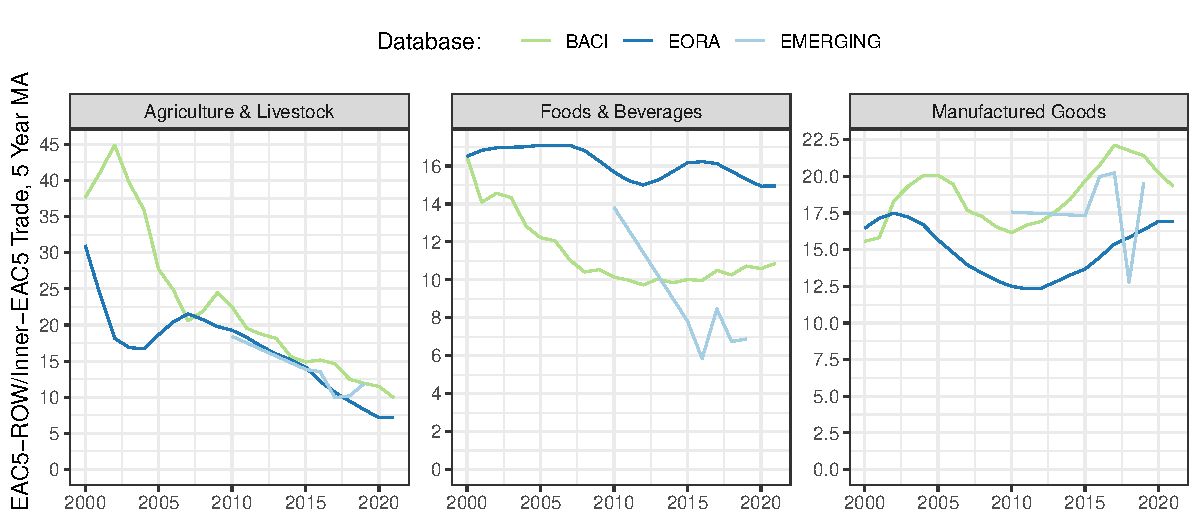
\includegraphics[width = \textwidth]{"../Figures/REV/ROW_EAC_Trade_Ratios_Sec_5YMA.pdf"}
\raggedright
\scriptsize 
\emph{Notes:} Figure shows the ratio of EAC5 $\Leftrightarrow$ ROW to inner-EAC5 trade (exports + imports), smoothed using a backward looking 5-year moving average. The EAC5 includes Tanzania, Kenya, Uganda, Rwanda and Burundi. The broad sectors shown are AFF (left), FBE (middle) and TEX-MAN (right) in Table \ref{tab:sec}.
\end{figure}

\newpage

Figure \ref{fig:GTEACsharesSec} offers a detailed breakdown of the sector-level EAC5 trade share for different members and the EAC5 as a whole. In Agriculture, the developments in Figure \ref{fig:EAC_ROW_Ratios_Sec} are proportionally reflected in exports and imports: in 2015-20, the EAC5 exported 12.6\% of agricultural exports to itself, up from 4.6\% in 1995-2000, and imported 19.3\%, up from 9.3\% in 1995-2000. The food and beverages export shares also rose from 7.8\% to 13.7\%, whereas the import share remained constant around 20\%. In manufacturing, the opposite is the case, with the EAC5 exports share declining from 32\% to 18.6\%, and the import share remaining roughly constant around 7\%. At the country-level, Uganda significantly increased its EAC5 share as an exporter and importer of both agricultural produce and foods and beverages. This development is mirrored, to a lesser extent, by Kenya, which additionally maintains a very high EAC5 share of manufactured exports of around 40\%, down from nearly 50\% in 2000. This stands in stark contrasted to a very small EAC5 import share of less than 1\%. Tanzania increased its export share to the EAC in all 3 broad sectors, while further decreasing its already low import shares in foods and manufactures to around 5\%. Rwanda and Burundi both have high export and import shares with the EAC5 in all sectors apart from manufacturing exports, but Rwanda strongly decreased its EAC5 agriculture and foods export shares since 2007, approaching the levels of Kenya in 2020, whereas Burundi strongly increased its agricultural export share from almost 0\% in 2005 to 60\% in 2020, while decreasing its import share from 70\% to 30\% over the same period. \newline 

Considering the different levels of developmet of these counties, the graph suggests that countries first become regional agricultural exporters, and later suppliers of manufactured goods. However, with the exception of foods and beverages, these manufactured goods do not appear to cater well to other members demands, as evidenced by the declining EAC5 shares in both exports and imports, and thus fail to become a driver of economic integration. Another problem appears to be the hegemonic position of Kenya as a supplier of manufactures, which may crowd out other countries attempts to increase their regional supply. Thus also at the bilateral-sector level, gross trade data suggests that EAC regional integration through trade is asymmetric, has progressed mainly via agricultural produce and foods and beverages, and is stronger in terms of exports than in terms of imports. %Particularly economically smaller countries like Rwanda, Burundi, and to a lesser extent Uganda, have significant trade shares with the EAC, particularly in imports. The 
Particularly the larger economies Tanzania and Kenya import much more from ROW. Among these 5 countries, Tanzania shows the overall lowest level of regional integration. 

\begin{figure}[h!] \vspace{-3mm}
\centering
\caption{\label{fig:GTEACsharesSec}\textsc{EAC5 Share in Members Gross Trade by Sector using BACI Data}}
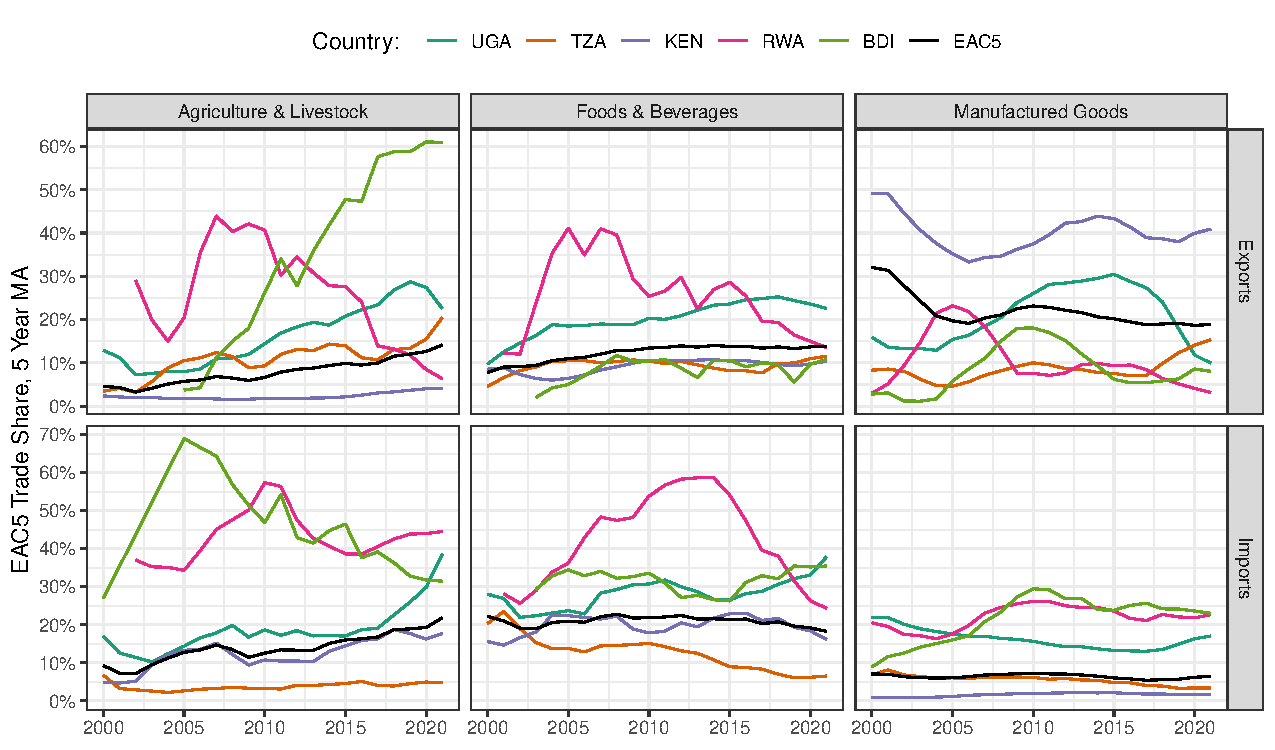
\includegraphics[width=\textwidth, trim= {0 0 0 0}, clip]{"../Figures/REV/GT_EAC5_shares_sec_ts.pdf"} % "../Figures/VA_EAC_shares_ts".pdf
\raggedright
\scriptsize 
\emph{Notes:} Figure shows the EAC5 share in members total exports and imports, smoothed using a backward looking 5-year moving average. The broad sectors shown are AFF (left), FBE (middle) and TEX-MAN (right) in Table \ref{tab:sec}.
\end{figure}
\FloatBarrier

An advantage of ICIO databases is that they record gross trade in both intermediates and final goods. Due to its greater accuracy, I only examine such flows using the EM database, averaged across years 2015-2019 to smooth temporal variation. Figure \ref{fig:wld} shows an aggregate intermediate flows table. The columns indicate intermediate inputs required by each country or region from each row country or region. Conversely, the rows indicate intermediate quantities supplied by each row country or region to each column country or region. \newline %Flows are reported on a log10 scale. \newline %due to their vastly different magnitudes.

Among the EAC countries, the table shows a significant supplier role of Kenya, supplying $10^{2.72} = 524$ million USD to Uganda, $10^{2.22} = 168$ million USD to Tanzania and  $10^{1.96} = 91$ million USD to Rwanda. Uganda/Tanzania also supply 258/228 million to Kenya, and 90/70 million to Rwanda. Tanzania supplies 56 million to Uganda, and Rwanda supplies 54 million to Kenya, all other inner-EAC intermediates trade is below 35 million.\footnote{Exempting South Sudan, which is subsumed in SSA because of data quality concerns, which receives 385 million in intermediates from Uganda and 223 million from Kenya.} EM estimates intermediate trade with ROW to be 27.3 times greater than inner-EAC trade, composed of intermediate inputs from ROW summing to 15.6 times EAC intermediates trade, and EAC inputs to ROW summing to 11.8 times EAC intermediates trade. The largest supplier of intermediates is China, supplying 831m to Uganda, 1937m to Tanzania, and 2704m to Kenya, followed by South Asia supplying 601/1066/1562, respectively, and the EU supplying 620/844/1462. Compared with these, the rest of SSA is relatively insignificant at 184/325/514. In terms of demand for EAC intermediates, the EU is the largest demander, demaning 552/828/1402, followed by the Middle East and North Africa (769/352/503), South Asia (101/683/618), the rest of SSA (105/716/462) and China (148/631/340). China, notably, supplies 4.9 times more intermediates than it demands from these three economies. Supply and demand of intermediates with the EU, NAC, and SSA is quite balanced. Overall, Uganda, Tanzania and Kenya combined demand 1.7 times more inputs from ROW than they supply. It should be noted that Congo, while not really integrated with other EAC members in terms of intermediates, has large and surprisingly balanced intermediate flows with ROW, demanding/supplying 2598/2636 with the EU and 1199/1375 with China. 

%	 assume less of a supplier role, with Tanziania supplying 12 million USD to Uganda, 40 million to Kenya, and 8 million to Rwanda, and Uganda supplying 8 million to Tanzania, 44 million to Kenya, and 34 million to Rwanda. Rwanda appears to be insignificant as a supplier, supplying less than 1 million USD in inputs to any of its EAC partners. Burundi and South Sudan appear insignificant both as suppliers and consumers of intermediates. With the rest of the world (ROW), Uganda, Tanzania, and Kenya each import between 250 and 800 million USD from the rest of SSA, and a similar magnitude from the Middle East, South Asia, and China. The largest supplier to EAC countries is the EU, supplying $10^{2.74} = 550$ million USD to Uganda, $10^{2.97} = 993$ million to Tanzania, $10^{3.44} = 2754$ million to Kenya, $10^{2.48} = 302$ million to Rwanda  $10^{1.96} = 91$ million to Burundi and $10^{1.11} = 13$ million to South Sudan. \newline 

\begin{figure}[h!] \vspace{-1mm}
\centering
\caption{\label{fig:wld}\textsc{Aggregated EMERGING MRIO Table: 2015-2019 Average}}
\small{\textit{Millions of Current USD at Basic Prices on a Log10 Scale}}
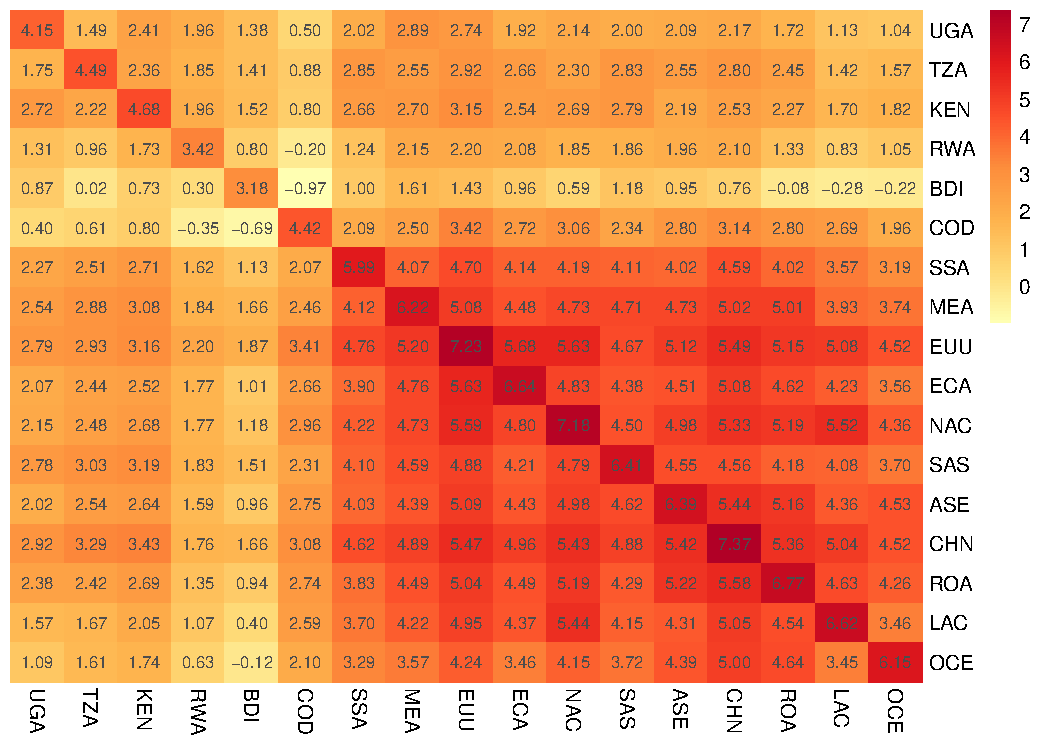
\includegraphics[width=1\textwidth, trim= {0 0 0 0}, clip]{"../Figures/REV/EM_heatmap_2015_19_AG.pdf"} \\ %trim={<left> <lower> <right> <upper>}
\raggedright
\scriptsize
\emph{Notes:} Figure shows gross intermediate input flows in log10 USD millions. Rows indicate the sources and columns the destinations of intermediates. The diagonal sums the domestic IO/regional ICIO table. 
\end{figure}
\FloatBarrier

Despite its high use of foreign inputs, domestic intermediate inputs corresponding to the diagonal entries, are on average 4.1 times greater than foreign inputs in EAC countries, and 6.3 times greater than EAC inputs to other countries. For the region as a whole, these figures are 4.6 and 6.13, respectively. This is low compared to other major regions, which produce and trade a lot more within themselves. For example, in the EU and North America, inputs from the region are around 10 times greater than foreign inputs. For China it is 14 times. \newline  %Gross intermediate flows thus establish that the EAC is substantially less integrated within itself than other world regions in terms of production.  \newline  

% This block somewhat duplicates the exercise with gross trade flows, but may be sensible for VA flows later on. 
%To better understand the relative magnitude of IO relationships within the EAC vis-a-vis ROW, Figure \ref{fig:outshares_ag_ts} plots three rations in gross and VA terms: ROW inflows into EAC production divided by EAC inputs into EAC production (excluding own country inputs), EAC inputs to ROW (outflow) also divided by EAC inputs to the EAC, and the EAC trade balance in intermediates, obtained by dividing the outflow ratio by the inflow ratio such that EAC inputs to the EAC cancel out. 
%
%% \todo[inline]{Driven by Tanzania? -> Nope !}
%\begin{figure}[h!] \vspace{-3mm}
%\centering
%\caption{\label{fig:TBint}\textsc{ROW/EAC Inflows and Outflows and Intermediates Trade Balance}}
%% \includegraphics[width=1\textwidth, trim= {0 0 0 0}, clip]{"../Figures/GROSS_RATIOS".pdf}
%\includegraphics[width=\textwidth, trim= {0 0 0 0}, clip]{"../Figures/ALL_RATIOS".pdf} %trim={<left> <lower> <right> <upper>}
%\raggedright
%\scriptsize
%\emph{Notes:} Inflow Ratio $=$ (ROW $\to$ EAC)/(EAC $\to$ EAC), Outflow Ratio $=$ (EAC $\to$ ROW)/(EAC $\to$ EAC),\\ \hphantom{Notes:.} Trade Balance in Intermediates Ratio $=$ (EAC $\to$ ROW)/(ROW $\to$ EAC). 
%\end{figure}
%\FloatBarrier
%
%Figure \ref{fig:TBint} signifies that the IO relationships of the EAC with ROW have developed asymmetrically. ROW stably supplies 12 times more inputs for EAC production than other EAC members, but EAC inputs for ROW production have declined relative to inner-EAC intermediate flows, from 5.9 in 2005 to 4.4 in 2015. This is reflected in the intermediates trade balance and implies that the EAC is becoming less important as a supplier of inputs for production abroad, while at the same time unable to replace intermediate imports from abroad with EAC intermediates. \newline


Figure \ref{fig:shares_ag} compactly summarizes the structure of production and trade in the EAC. Domestic value added (VA) is around 60\% of output in all EAC members apart from Rwanda where it is 73\%. The other components of output are domestic and imported intermediates, of which, as the second plot shows, between 17 and 24\% are imported by different EAC members. Gross output is then either consumed or exported for either intermediate or final use. The RHS of Figure \ref{fig:shares_ag} shows that between 5 and 16\% of gross output are exported by EAC members. 
%Figure \ref{fig:outshares_ag_ts} provides a broader view of gross EAC production and trade, showing the shares of domestic VA (VAS) and imported inputs in gross output, alongside the share of output exported, and the shares of exports/imports to/from EAC members over the 2005-2015 period. VAS is at 50-60\% of gross output for all EAC countries apart from Tanzania\footnote{Likely due to inconsistencies in GDP data for Tanzania.} and South Sudan. 
\begin{figure}[h!] \vspace{-1mm}
\centering
\caption{\label{fig:shares_ag}\textsc{Gross Decomposition of EAC Production and Trade}}
\vspace{2mm}
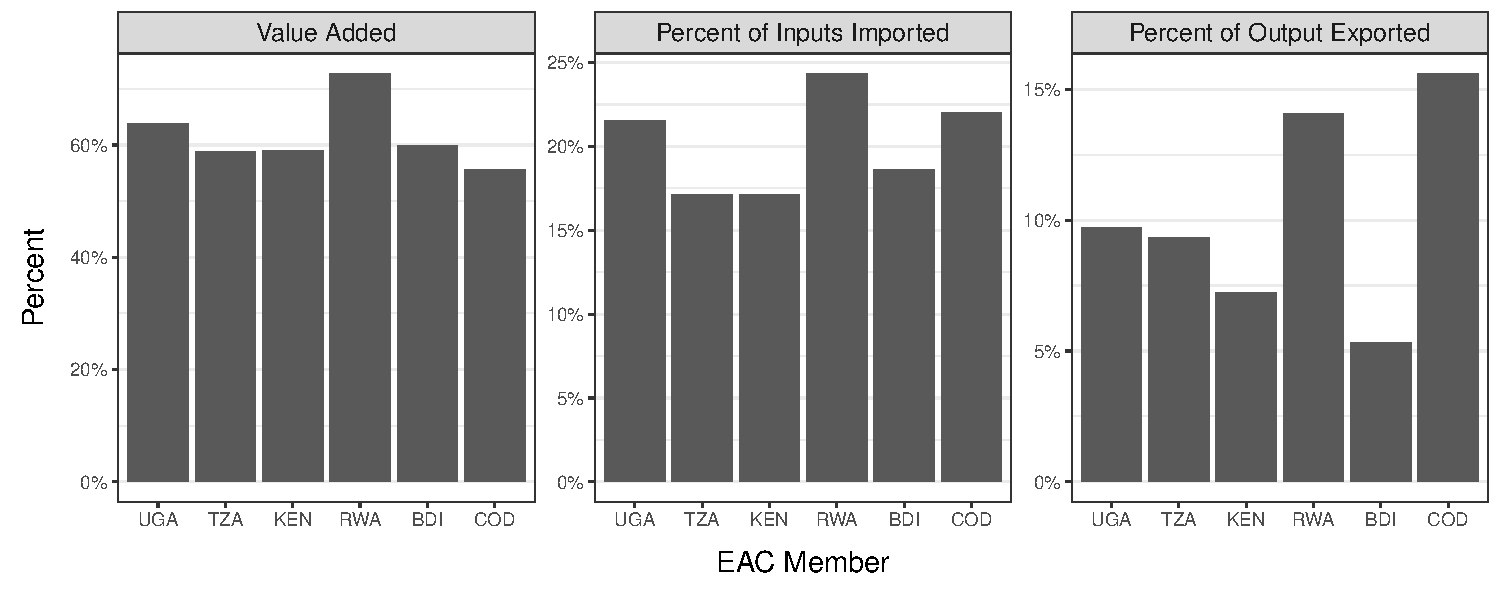
\includegraphics[width=1\textwidth, trim= {0 1cm 0 0}, clip]{"../Figures/REV/EM_gross_shares_ag.pdf"} % output_shares_ag_ts
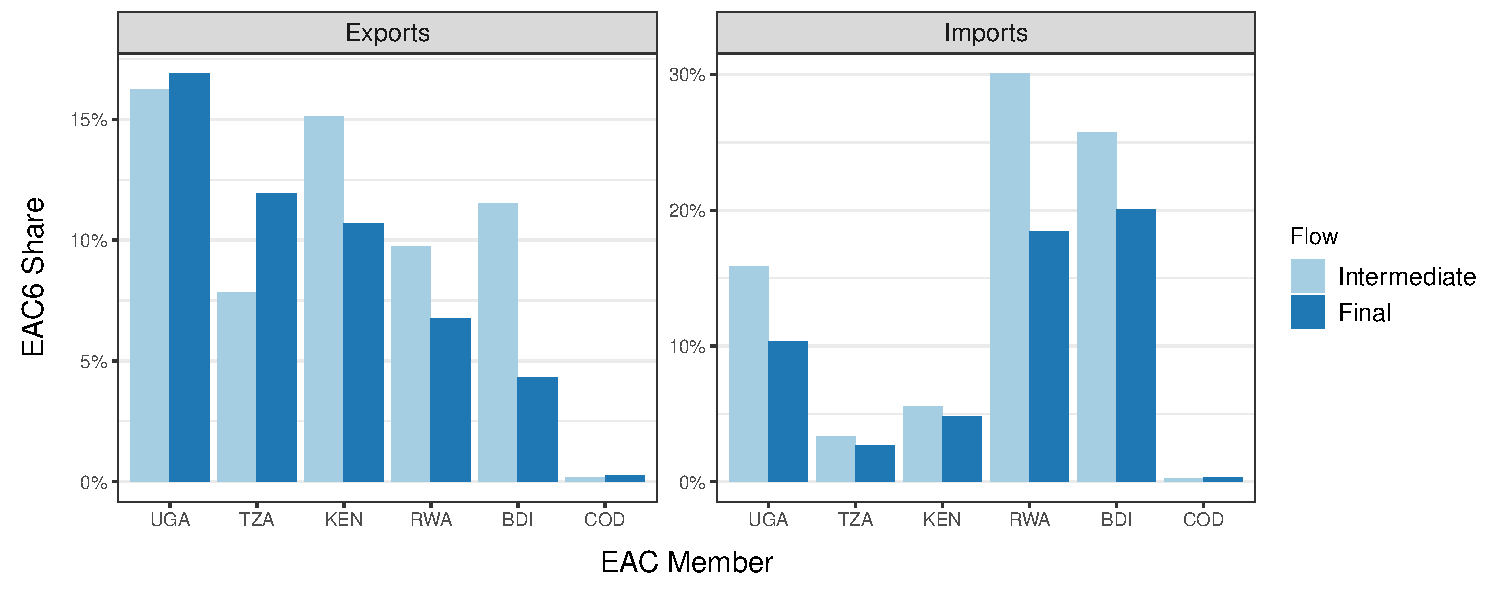
\includegraphics[width=1\textwidth, trim= {0 0 0 0}, clip]{"../Figures/REV/EM_gross_trade_shares_ag.pdf"} \\
\raggedright
\scriptsize
\emph{Notes:} Based on EMERGING and computed using an 2015-2019 average MRIO table. 
\end{figure}
\FloatBarrier

The bottom panel of Figure \ref{fig:shares_ag} decomposes exports and imports by type of flow. It shows that three countries, Uganda, Rwanda and Burundi have significant export and import shares for both intermediate and final products with the EAC. Kenya and Tanzania on the other hand export significant amounts to the EAC but only import small shares. With the exception of Tanzanian and Ugandan exports, inner-EAC trade in intermediates is slightly larger than trade in final goods. \newline

%The remainder of output (1-VAS) is comprised of domestic or imported intermediate goods. The 'Percent of Inputs Imported' is a gross measure of backward GVC integration, and less than 10\% in all EAC countries exempting Tanzania. Kenya appears to have the highest level at 10\% of inputs imported. Of the imported inputs, the 'Percent of Imports from EAC' signifies another asymmetry in EAC economic integration: whereas Uganda has both exports and import shares of 25-30\% with the EAC, Kenya only exports close to 30\%, with EAC share in imports at 2\%. In contrast, Rwanda imports 12-15\% from the EAC, but exports very little at $\sim$2\%. Other countries have both export and import shares below 10\%. Apart from Kenya and Uganda exporting more to the EAC over time, Figure \ref{fig:outshares_ag_ts} shows little aggregate development regarding EAC regional and global integration in gross terms. Appendix Figure \ref{fig:exp_EAC_share} gives a sector-level breakdown of the percentage of gross exports to other EAC countries. Uganda and Kenya both have export shares of 30\% with the EAC, but in Uganda, the largest part of these exports are agricultural, while in Kenya the largest part is manufacturing, in particular petrochemicals, metal products, and electric machinery. % The other EAC members don't export very much to the EAC, in particular Rwanda, Burundi, and South Sudan where the data suggests an EAC export share below 2\% in 2015. 
%

To end the examination of gross flows, Appendix Table \ref{tab:weaclfl} provides the 50 largest sector-level intermediate flows (excl. Congo). Both with ROW and inside the EAC, the largest intermediate flows are in manufacturing, and in particular, in petrochemicals (PCM), foods and beverages (FBE), and, to a lesser extent, textiles (TEX). %Tanzania also has some electrical machinery (ELM) with larger input from China. 
Kenya is a significant EAC supplier of manufacturing inputs, particularly for PCM, FBE and metal product (MPR) industries. Kenya also supplies large transport (TRA) (including travel and tourism) intermediates to EU transport (tourism) services, and agricultural inputs to EU FBE industries. It also supplies large inputs for FBE industries in South Asia. These flows are on average 3-4 times larger than its regional intermediate supplies. Uganda supplies PCM to ROW, and FBE and agriculture to Kenyan FBE and TRA industries. 


\section{Value Added Flows}

While gross flows provide useful information about direct productive relationships, they do not reveal how much of the value was added in the supplying country-industry and previous production stages performed by other country-industries. % \citep{Kummritz2014}. 
The Leontief decomposition solves this problem by reallocating the value of intermediate inputs to the original producers \citep{Kummritz2014}. To guide the further discussion of VA trade flows I begin with some formal derivations and introduce a consistent notation used throughout this paper. \newline

% \subsection{The Leontief Decomposition}

Let $\textbf{A}$ be a normalized ICIO table where each element $a_{oi,uj}$ gives the units of origin country $o$ and sector $i$'s (row) output required for the production of one unit of using country $u$ and sector $j$'s (column) output, $\textbf{x}$ the vector of outputs of each country-sector, and $\textbf{d}$ a vector of final demands such that the following productive relationship holds

\begin{equation} \label{eq:io_model}
\textbf{x} = \textbf{A}\textbf{x} + \textbf{d}.
\end{equation}

The classical \citet{leontief1936quantitative} insight was that one can solve this equation for $\textbf{x}$ to get the amount of output each country-sector should produce given a certain amount of final demand

\begin{equation} \label{eq:leontief}
\textbf{x} = (\textbf{I}-\textbf{A})^{-1} \textbf{d} = \textbf{B}\textbf{d},
\end{equation}

\noindent where the Leontief Inverse in denoted $\textbf{B} = (\textbf{I}-\textbf{A})^{-1}$. This matrix is also often called the total requirement matrix since it gives the total productive input requirement from each sector to produce one unit of final output\footnote{Specifically each element in $b_{oi,uj}$ in \textbf{B} gives the output required from country-sector $oi$ for the production of one unit of the final good in $uj$. Thus the first column of \textbf{B} gives all the productive input required from all sectors for the production of one unit of the final good in sector 1, and the first row of \textbf{B} gives all the input required from sector 1 to produce one unit of the final good in each sector.}. The direct VA share of each country-sector is given by

\begin{equation}
\textbf{v} = \textbf{1} - \textbf{A}'\textbf{1},
\end{equation}

where $\textbf{1} = (1, 1, 1, ..., 1)'$ is a column-vector of 1's\footnote{Thus the expression amounts to summing up the entries in each column of \textbf{A} (representing the intermediate input shares for 1 unit of output) and subtracting them from 1.}. Let \textbf{V} be the matrix with \textbf{v} along the diagonal and 0's in the off-diagonal elements. Multiplying Eq. \ref{eq:leontief} with $\textbf{V}$ then gives VA in each country-sector

\begin{equation} \label{eq:VB}
\textbf{V}\textbf{x} = \textbf{V}(\textbf{I}-\textbf{A})^{-1} \textbf{d} = \textbf{VBd}.
\end{equation}

The term $\textbf{VB} = \textbf{V}(\textbf{I}-\textbf{A})^{-1}$ is known as the matrix of VA multipliers or VA shares, which can be used to obtain the amount of VA generated in each sector (\textbf{Vx}) when producing to satisfy final demand (\textbf{d}). More specifically, the matrix $\textbf{VB}$ contains the amount of VA by each country-sector (row) to the production of one unit of each country-sector's (column's) output. 


\subsection{Backward GVC Participation}

The foreign VA share in domestic production and exports, termed 'Vertical Specialization' (VS) by \citet{hummels2001nature}, is the most widely used measure of backward GVC integration. Consider \textbf{VB} with elements vb$_{oi,uj}$, then VS for a particular country-sector may be expressed as\footnote{In words: sum the elements of \textbf{VB} in each column, excluding domestic country-sectors.}

\begin{equation} \label{eq:VS}
\text{VS}_{uj} = \sum_{oi,\ o \neq  u} \text{vb}_{oi, uj}\ \ \forall uj.
\end{equation}

Figure \ref{fig:EACVB_ag_ts} shows a time series of VS according to different data sources. The calculated VS measure using EORA21 is identical to the WDR one. The extension of EORA through 2021, as mentioned, introduces a large structural break in 2016, which, in some cases such as Tanzania where VS drops to zero or Burundi where VS rises to above 50\% (truncated in Figure \ref{fig:EACVB_ag_ts}) is highly unrealistic. As mentioned, EM is the more reliable database for these countries, and indicates that for all EAC members between 8\% and 30\% of gross exports is foreign content. Furthermore, EM suggests that the smaller economies Burundi, Rwanda and Uganda have increased their VS, especially in 2015-2019, whereas Kenya and Congo have seen a decline in VS. in Tanzania, VS appears stagnant around 16\%. 

\begin{figure}[h!]
\centering
\caption{\label{fig:EACVB_ag_ts}\textsc{EAC Backward GVC Participation}}
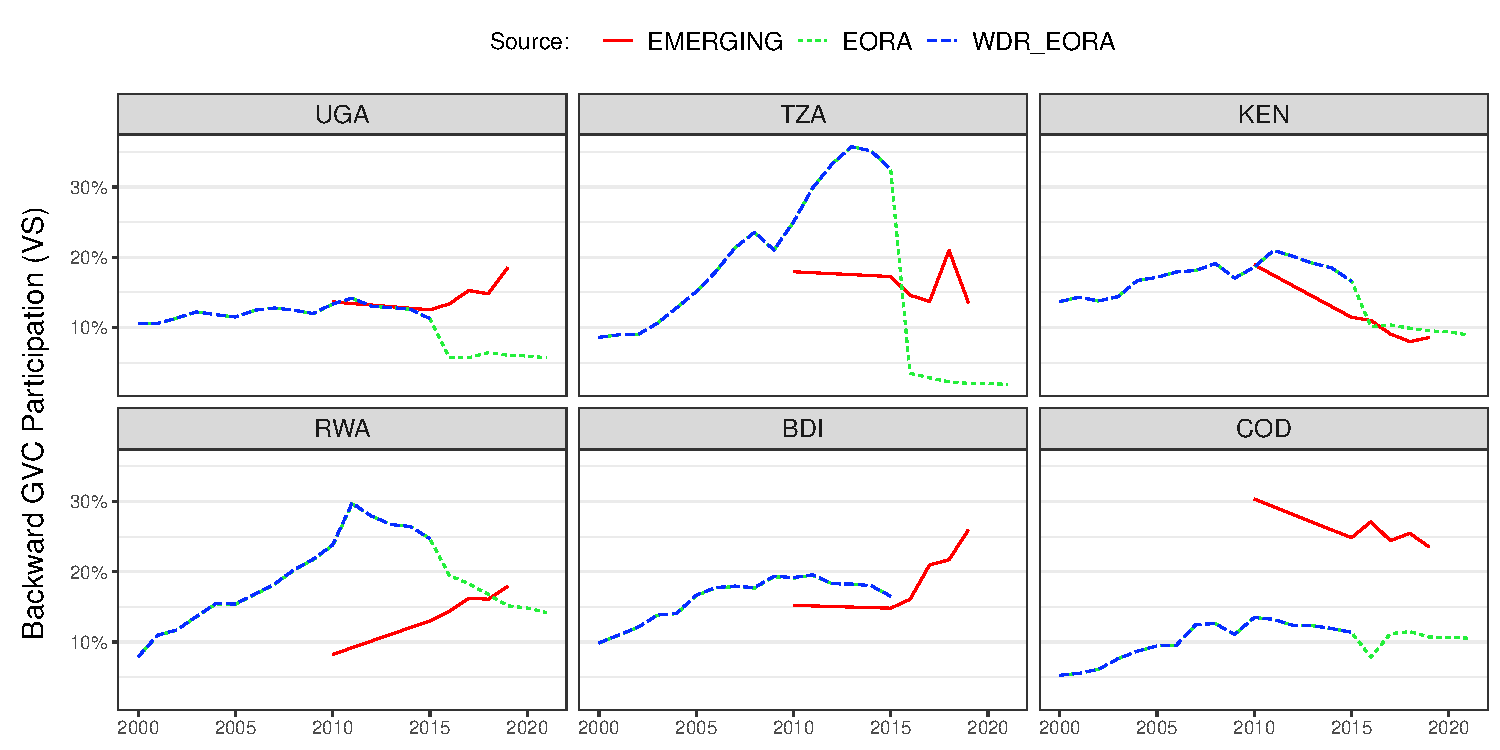
\includegraphics[width=1\textwidth, trim= {0 0 0 0}, clip]{"../Figures/REV/VA_shares_ag_ts.pdf"} %trim={<left> <lower> <right> <upper>}
\raggedright
\scriptsize
\emph{Notes:} \citet{hummels2001nature}'s index of Vertical Specialization (VS) is the foreign VA share in gross output and exports. 
\end{figure}
\FloatBarrier

Apart from its overall size, the composition of the foreign content of exports (and production in the ICIO framework) at the country and sector levels is of interest. Figure \ref{fig:EACVB_ctry} shows a breakdown of foreign content by source country/region, averaged, for EORA, between 2010 and 2015, and for EM between 2015 and 2019. Figure \ref{fig:EACVB_ctry} indicates that, in line with the EAC import share shown in the bottom right panel of Figure \ref{fig:shares_ag}, only Rwanda, Burundi and Uganda source a significant fraction of foreign inputs from EAC partners. According to EM, Kenya supplies 11.5\% of the foreign content in Ugandan exports, 9.8\% in Rwanda, and 8\% in Burundi. Uganda also supplies 9.3\% of the foreign content in Rwandan exports, and 5.5\% in Burundi. In absolute values, Uganda supplies slightly more to Kenyan export production (around 23 million USD according to EM, vs. 20.7 million to Rwanda). This is dwarfed by the 115 million that Kenya supplies for Ugandan export production. \newline 

Overall, the EU and China are the greatest suppliers of foreign content in EAC exports, supplying, in the case of the EU, 33\% of the foreign content of Congolese exports, 23\% in Burundi, 21\% in Rwanda, 17\%, 16\%, 15\% in Uganda, Kenya and Tanzania, respectively. China supplies 27\% of the foreign content of Kenyan and Tanzanian exports (approx. 300 million USD in both cases), 21\% in Uganda, and 16\% in Congo. Thus overall EAC exports have modest amounts of foreign content and most of this foreign content, particularly for major exporters Congo, Kenya and Tanzania, is accounted for by the EU and China. 

\begin{figure}[h!]
\centering
\caption{\label{fig:EACVB_ctry}\textsc{EAC Backward GVC Participation: Sources of Foreign Content}}
\small{\textit{Average EMERGING 2015-2019 Foreign Content Share in Parentheses}}
\vspace{2mm}
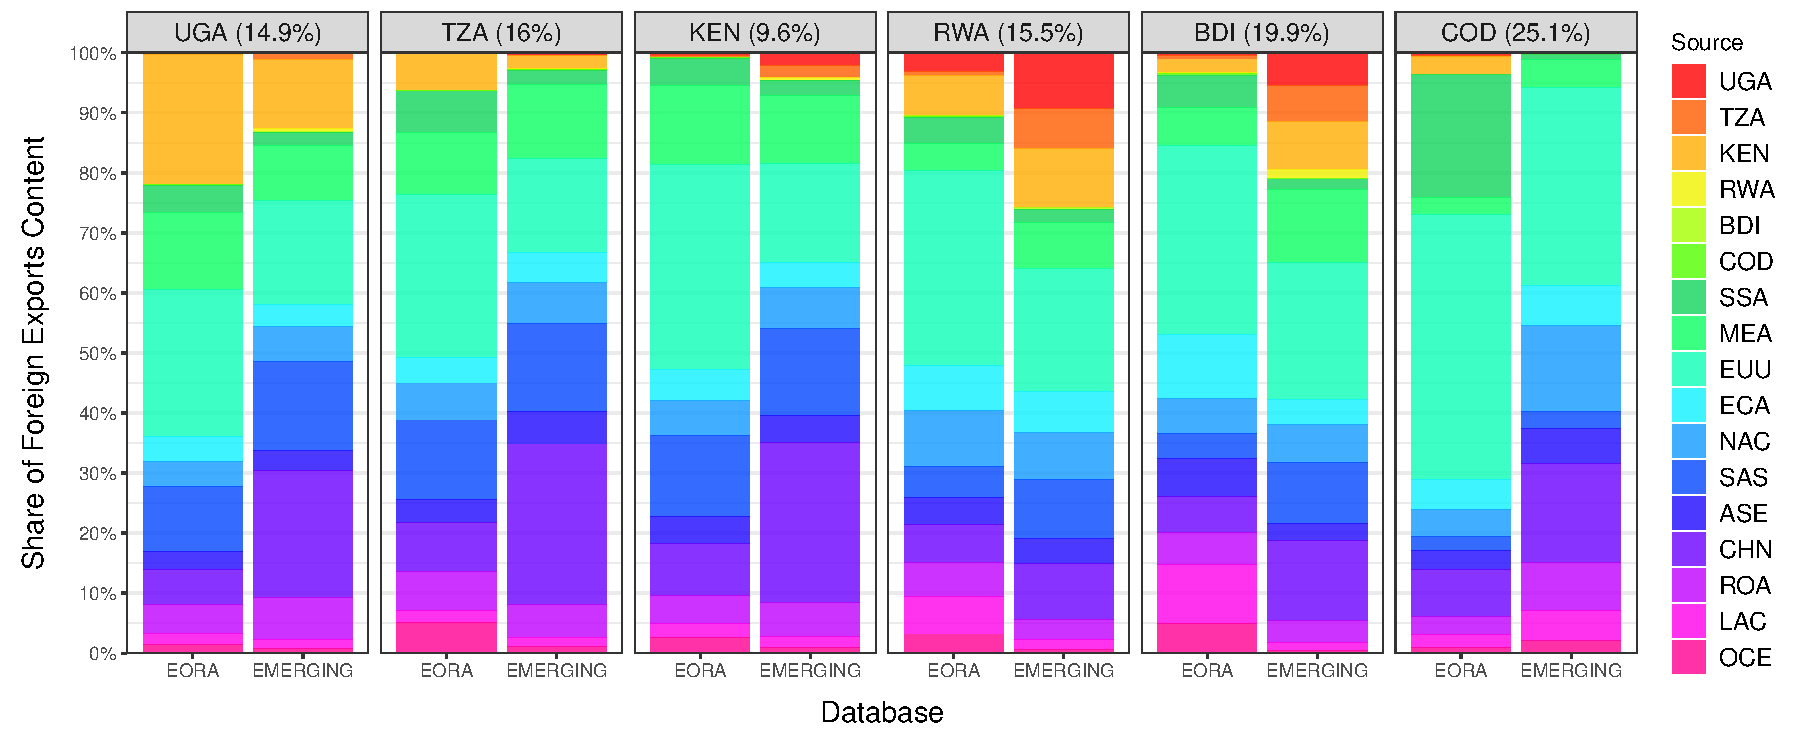
\includegraphics[width=1\textwidth, trim= {0 2mm 0 0}, clip]{"../Figures/REV/VA_shares_ctry.pdf"} \\ %trim={<left> <lower> <right> <upper>}
\raggedright
\scriptsize
\vspace{-2mm}
\emph{Notes:} Figure shows a breakdown of VS by source country, according to EORA (2010-2015) and EM (2015-2019) averages. \\ \vspace{-5mm}
\end{figure}
\FloatBarrier

%Figure \ref{fig:EACVB_ts} displays a breakdown of VS for EAC countries by supplier country-region over the analyzed period. In Uganda, VS has been fluctuating between 10 and 12\%. 2\% of the value of Ugandan produce comes from Kenya, about 1\% from the rest of SSA, 1.5\% from MEA, about 3-4\% from EUU, and 1-1.5\% from SAS. The other regions make up the remaining 2\%. Tanzania and Kenya have similar relative VA contributions of SSA, MEA, EUU, and SAS regions to their production, at overall higher foreign content shares, e.g. VS of 16\% in Kenya. Data for Tanzania and Rwanda show stark trends, but these should be interpreted in light of the data quality\footnote{Particularly the declining GDP estimate of Tanzania (Figure \ref{fig:EAC_GDP_sec}) seems to encourage higher foreign VA to compensate for rising exports (Figure \ref{fig:exp}). Figure \ref{fig:VSag_ts_21} shows that in the extended database VS drops starkly in 2016, lending further support to this interpretation.}. Kenya adds around 1-2\% to Tanzanian output, and Uganda adds about 0.1\% to Kenyan output. The VA share of Kenya and Uganda in Rwandan production of around 1\% and 0.5\% respectively is also clearly visible. It is noteworthy that overall VS appears to have declined in Uganda, Kenya, Rwanda, and Burundi from 2011 onwards. Appendix Figure \ref{fig:EACVB_ts_bar} further shows bars providing the VA share in 2005 and 2015 and their difference. Kenya's VA share has increased slightly in all EAC countries between 2005 and 2015\footnote{%(except for South Sudan\footnote{The data for South Sudan is unreliable, also minding that the country only became independent in 2011.}), 
%Amounting to an increase of 0.17 percentage points of gross output in Uganda, 0.89 percentage points in Tanzania, 0.29 percentage points in Rwanda, and 0.03 percentage points in Burundi.}. Rwanda has also seen increases in the shares of Ugandan VA of around 0.14 percentage points. % All of this indicates that Kenya is becoming a more important supplier of inputs for EAC production, but that integration into regional and global value chains is stagnant otherwise. 
%\begin{figure}[h!]
%\centering
%\caption{\label{fig:EACVB_ts}\textsc{Foreign Value Added Shares in EAC Production (VS)}}
%\includegraphics[width=1\textwidth, trim= {0 0 0 0}, clip]{"../Figures/VA_shares_ag_ts_area".pdf} %trim={<left> <lower> <right> <upper>}
%\end{figure}
%\FloatBarrier

Different sectors exhibit great heterogeneity, both in terms of overall foreign content and its composition. Table \ref{tab:EACVB_sec} shows overall sectoral foreign content shares according to EM. In general, manufacturing sectors have higher foreign content, a pattern noted in the WDR, which also notes that a handfull of sectors, including electrical machinery and transport equipment, drove GVC expansion since 1995. In the average EAC country these manufacturing sectors have more than 20\% foreign content, but there is marked heterogeneity across countries. Notably, in Rwanda manufacturing sectors have less than 15\% foreign content. The highest foreign content sectors by country are electrical machinery in Tanzania (42\%), wood and paper in Kenya (40\%) mining and textiles in Uganda (29\%), sales and repairs in Rwanda (25\%), petro-chemicals in Burundi (47\%) and transport equipment in Congo (36\%). Since Burundi and Congo have no IO table, these figures need to be taken with caution. The final columns of Table \ref{tab:EACVB_sec} give FVA in overall sectoral exports by EAC members, including value addition by other members, with and without Congo. These resemble a classical VS distribution, centering around ELM and TEQ at $\sim$ 35\%. 

%\begin{figure}[h!]
%\centering
%\caption{\label{fig:EACVB_sec}\textsc{EAC Backward GVC Participation: Sectoral Heterogeneity}}
%\small{\textit{Average EMERGING 2015-2019 Foreign Content Shares}}
%% \small{\textit{Average EMERGING 2015-2019 Foreign Content Share in Parentheses}}
%\vspace{2mm}
%\includegraphics[width=1\textwidth, trim= {0 0 0 0}, clip]{"../Figures/REV/VA_shares_sec.pdf"} %trim={<left> <lower> <right> <upper>}
%\end{figure}
%\FloatBarrier

% latex table generated in R 4.3.0 by xtable 1.8-4 package
% Tue Jan  9 19:37:21 2024
\begin{table}[ht] \vspace{-2mm}
\centering
\caption{\label{tab:EACVB_sec}\textsc{EAC Backward GVC Participation: Sectoral Heterogeneity}}
\small{\textit{Average EMERGING 2015-2019 Foreign Content Shares}} \\
\vspace{1mm}
\begin{tabular}{lrrrrrrrrrr}
  \toprule
sector & UGA & TZA & KEN & RWA & BDI & COD & Mean & Median & EAC6 & EAC5 \\ 
  \midrule
AFF & 5.9 & 4.1 & 3.7 & 5.8 & 15.2 & 3.3 & 6.3 & 5.0 & 4.2 & 4.4\\ 
  MIN & 29.2 & 5.5 & 0.0 & 2.0 & 17.0 & 4.7 & 9.7 & 5.1 & 4.6 & 6.8\\ 
  FBE & 22.7 & 7.6 & 3.1 & 20.6 & 19.3 & 13.6 & 14.5 & 16.4 & 11.1 & 10.7\\ 
  TEX & 29.6 & 17.1 & 25.2 & 8.3 & 8.5 & 28.6 & 19.6 & 21.2 & 26.1 & 24.1\\ 
  WAP & 13.7 & 22.7 & 39.5 & 1.4 & 5.9 & 20.1 & 17.2 & 16.9 & 24.8 & 29.2\\ 
  PCM & 23.9 & 19.8 & 19.5 & 10.2 & 47.1 & 20.6 & 23.5 & 20.2 & 20.0 & 19.7\\ 
  MPR & 27.0 & 26.9 & 16.2 & 10.2 & 39.7 & 25.0 & 24.2 & 26.0 & 24.3 & 23.6\\ 
  ELM & 18.7 & 41.9 & 30.7 & 5.2 & 27.4 & 34.9 & 26.5 & 29.1 & 34.9 & 35.2\\ 
  TEQ & 22.7 & 17.1 & 19.7 & 0.0 & 32.8 & 36.4 & 21.4 & 21.2 & 34.6 & 23.9\\ 
  MAN & 23.3 & 21.8 & 27.3 & 0.8 & 0.4 & 24.5 & 16.3 & 22.6 & 25.3 & 25.6\\ 
  EGW & 28.2 & 3.1 & 26.2 & 0.0 &  & 2.1 & 11.9 & 3.1 & 16.9 & 27.1\\ 
  CON & 15.6 & 13.1 & 16.2 & 7.4 & 5.3 & 30.6 & 14.7 & 14.3 & 12.9 & 12.9\\ 
  SMH & 5.6 & 11.7 & 9.4 & 25.2 & 14.1 & 15.3 & 13.5 & 12.9 & 10.9 & 10.9\\ 
  TRA & 7.6 & 18.5 & 6.6 & 4.7 & 0.1 & 4.3 & 7.0 & 5.7 & 11.0 & 11.0\\ 
  PTE & 11.0 & 21.7 & 5.4 & 0.0 & 0.0 & 2.5 & 6.8 & 4.0 & 11.9 & 12.0\\ 
  FIB & 0.4 & 8.2 & 0.3 & 1.9 & 0.0 & 4.5 & 2.5 & 1.1 & 1.1 & 0.9\\ 
  PAO & 5.0 & 2.2 & 8.0 & 0.0 & 0.0 & 4.5 & 3.3 & 3.4 & 6.8 & 7.0\\ 
   \bottomrule  \\ [-0.9em]
\multicolumn{11}{l}{\parbox{0.85\textwidth}{\scriptsize
\textit{Notes:} Table reports total foreign content shares (VS) according to the EM 2015-2019 average in percentage terms. These shares are reported for each EAC6 country, and for the EAC6 and EAC5 as a whole, which also counts VA by members amog each other as foreign VA, i.e., these are export-weighted averages of individual members VS. The 'Mean' and 'Median' give unweighted EAC6 averages.}}
\end{tabular}
\end{table}

 Figure \ref{fig:EACVB_ctry_sec} breaks down the origin of the EAC5 FVA, and thus provides a sector-level perspective of EAC regional integration. According to Figure \ref{fig:EACVB_ctry_sec} the sectors with the highest EAC FVA

\begin{figure}[h!] \vspace{-2mm}
\centering
\caption{\label{fig:EACVB_ctry_sec}\textsc{EAC5 Backward GVC Participation: Sources of VS by Sector}}
\small{\textit{Based on Average EMERGING 2015-2019 EAC Exports (Excl. Congo)}}
\vspace{2mm}
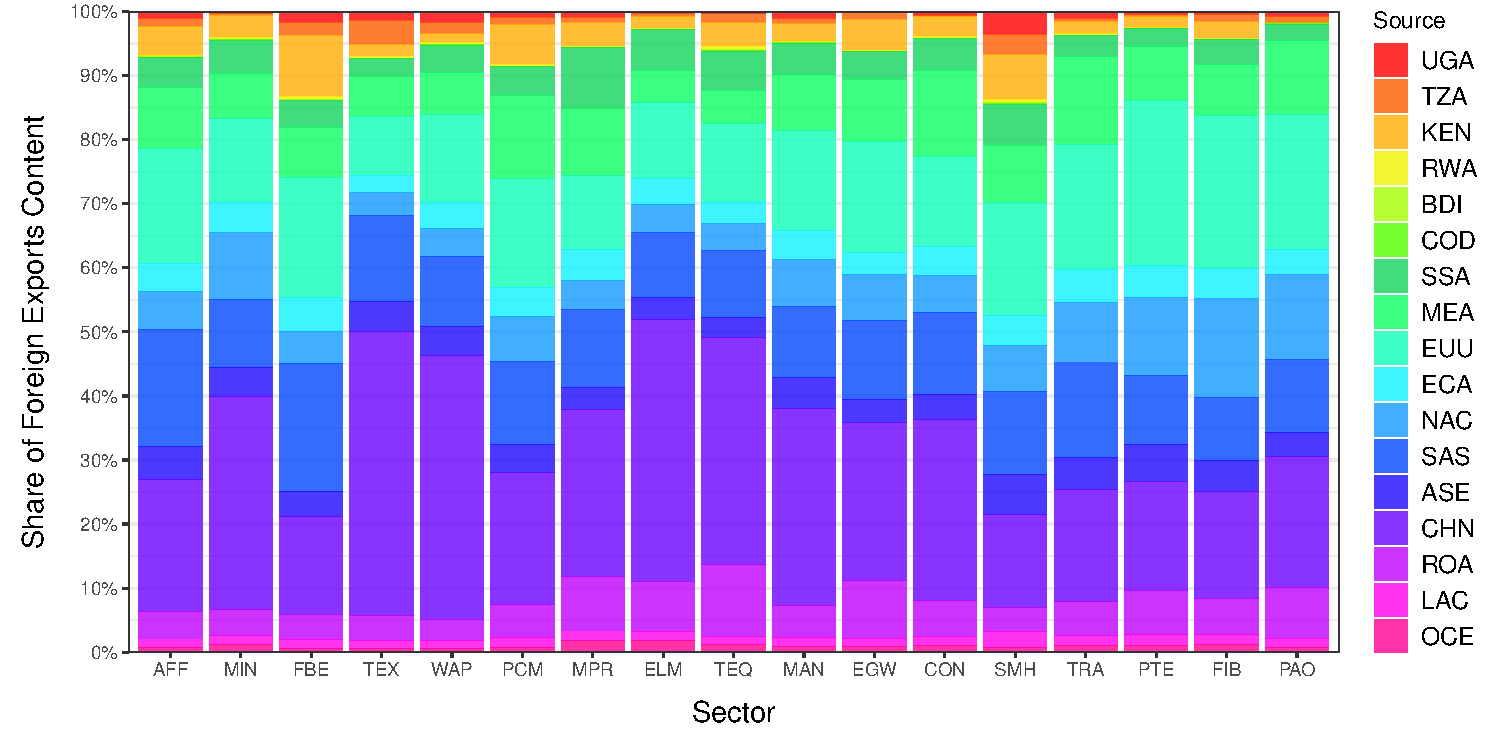
\includegraphics[width=1\textwidth, trim= {0 0 0 0}, clip]{"../Figures/REV/VA_shares_sec_ctry.pdf"} \\ %trim={<left> <lower> <right> <upper>}
\raggedright
\scriptsize
\vspace{-3mm}
\emph{Notes:} Figure shows a sector-level breakdown of total EAC5 VS by source country, according to EM (2015-2019) averages. \\ \vspace{-10mm}
\end{figure}
\FloatBarrier 
\noindent share are sale and repair of vehicles, fuel trade and hotels (SMH) at 14.5\% and food and beverages (FBE) at 14\%. Other sectors with sizeable shares are petrochemicals (PCM) at 8.6\%, textiles at 7.4\%, agriculture (AFF) at 7.2\%, electricity (EGW) at 6.3\% and transport equipment at 6.2\%. This highlights quantitatively the potential of the food processing sector for regional integration, but also indicates a failure of regional integration in many core manufacturing sectors. For example the electrical machinery (ELM) sector, which has a FVA content around 35\% according to Table \ref{tab:EACVB_sec}, only has a 2.8\% regional FVA share. Multiplying these percentages yields that only 1\% of the gross output (and exports) in EAC ELM is regional FVA, compared to 1.5\% for FBE. \footnote{Given the lower FVA share of 11\% in the FBE sector.} Figure \ref{fig:EACVB_ctry_sec} is thus indicative of great potential and challenges developing regional manufacturing value chains. 



\subsection{Forward GVC Participation}

Apart from VS, which measures backward GVC integration, \citet{hummels2001nature}, and more formally \citet{daudin2011produces}, introduced the share of domestic exports that enter foreign countries' exports, termed VS1, as a measure of forward GVC Integration. It is defined as\footnote{For completeness I note that VS can be defined in an analogous way as $\text{VS}_{uj} = \frac{1}{E_{uj}} \sum_{oi, o \neq  u} \text{vbe}_{oi, uj}\ \ \forall\ uj$, however, since $\sum_{oi} \text{vb}_{oi, uj} = 1\ \forall\ uj$, the exports cancel out and the equation reduces to Eq. \ref{eq:VS}. \vspace{-6mm}}
\begin{equation} \label{eq:VS1}
\text{VS1}_{oi} = \frac{1}{E_{oi}} \sum_{uj, u \neq  o} \text{vbe}_{oi, uj}\ \ \forall\ oi,
\end{equation}
\noindent where $E_{oi}$ are the gross exports of country-sector $oi$ used to normalize the sum along the rows of \textbf{VBE} (excluding domestic sectors) which capture the use of VA from a domestic sector $oi$ in the exports of all foreign sectors $uj$. \citet{borin2019measuring} show that this measure is biased because it contains double-counted components. They propose (DVA - DAVAX)/E, which is the ratio of domestic VA (excl. double counted items) minus directly absorbed domestic value added in exports (DAVAX) to gross exports as a refined measure of forward GVC participation. \newline 

Accurate computation of forward GVC participation requires a full country-level ICIO database. Due to computational constraints, I reduce the number of sectors to 5: AFF, FIB, MIN, MAN (combining 7 manufacturing sectors) and SRV (all other sectors), while preserving the full number of countries and territories (187 for EORA and 245 for EM). Figure \ref{fig:EAC_E2R_ag_ts} shows the corrected measure of forward GVC participation following \citet{borin2019measuring}. Evidently, a reduction of the sectoral dimension attenuates aggregate VS1 indicators a bit, but the trends are broadly preserved.  
% Evidently, the classical VS1 measure induces some upward bias\footnote{Which is due to double counted items but may also be partly affected by the reduced sector dimension.}, but follows the same trend as the corrected measure available in the WDR up to 2015. 
All indicators shows that commodity exporters such as Congo and Burundi have higher levels of forward GVC integration. The EMERGING measures suggest that VS1 has increased slightly in Congo, and decreased slightly in Kenya, Rwanda, and Tanzania since 2010, indicating a slight shift away from commodities in these economies. 

\begin{figure}[h!] \vspace{-1mm}
\centering
\caption{\label{fig:EAC_E2R_ag_ts}\textsc{EAC Forward GVC Participation}}
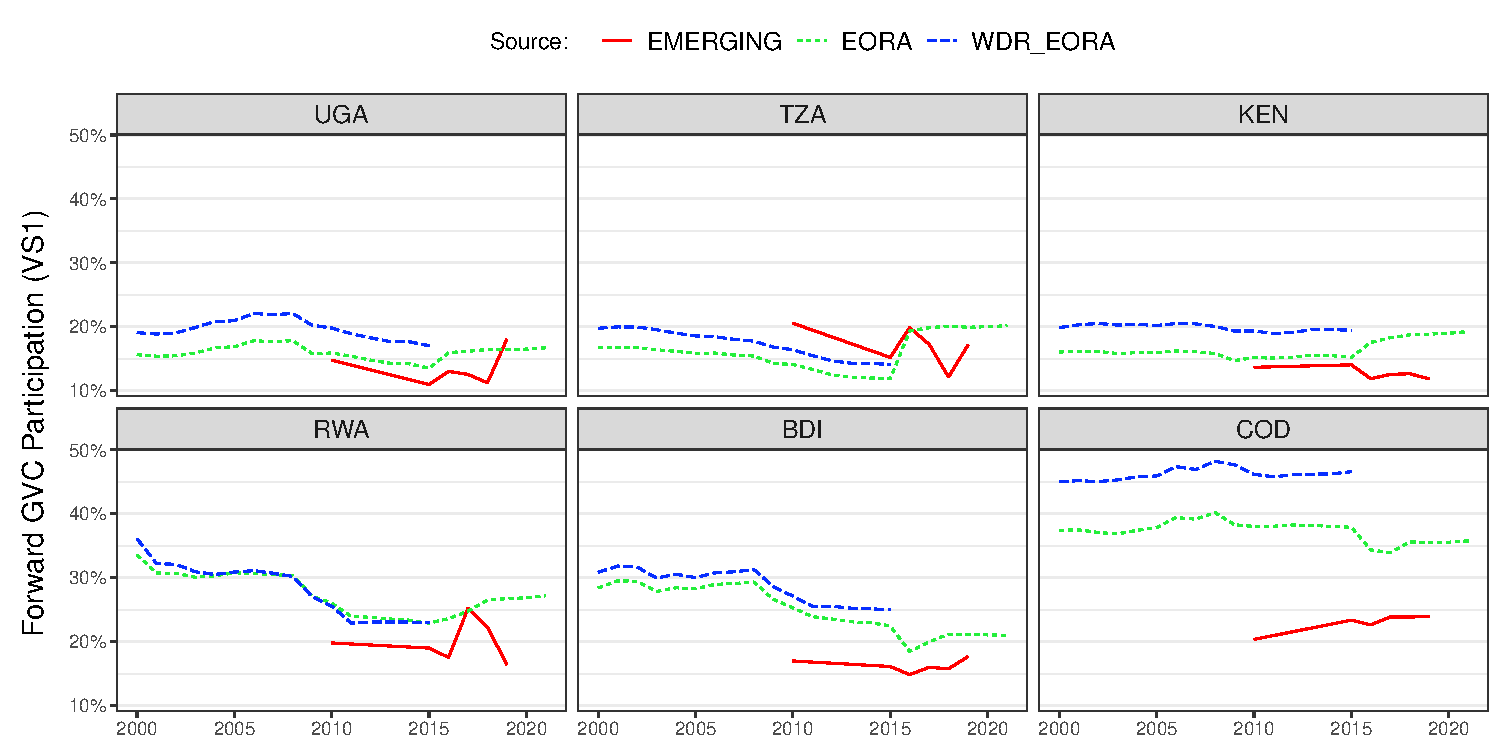
\includegraphics[width=1\textwidth]{"../Figures/REV/GVCF_shares_ag_ts.pdf"} \\ % VS1_shares_ag_ts.pdf
\raggedright
\scriptsize
% \vspace{-2mm}
\emph{Notes:} \citet{borin2019measuring}'s index of forward GVC intergration (VS1) is the (non-double counted) domestic VA in exports that is not directly absorbed by the direct importer, divided by gross exports: (DVA - DAVAX)/E. 
\end{figure}
\FloatBarrier
% \todo[inline]{Also report gross exports decomposition under gross flows.}

Since even with the 5-sector ICIO tables bilateral GVC indicators with \citet{belotti2020icio}'s ICIO package are extremely time consuming, I also compute the classical VS1 measure (also called exports to re-exports, short E2R by \citet{baldwin2015supply}) following Eq. \ref{eq:VS1} to examine bilateral relationships. Figure \ref{fig:EACVS1_ctry} shows a breakdown of VS1 by GVC partner. The headers show that E2R (Eq. \ref{eq:VS1}) is indeed upward biased vis-a-vis the corrected measure of \citet{borin2019measuring} (BM). Figure \ref{fig:EACVS1_ctry} indicates that, according to EMERGING, 4.4\% of Kenya's VS1 was re-exported by Uganda, and 3.2\% of Ugandan VS1 is re-exported by Kenya. Other EAC countries also re-export a small share of their re-exported exports through Kenya: Burundi (1.25\%), Rwanda (1.5\%), and Tanzania (1.5\%). Burundi and Rwanda have 2.4\% and 0.8\% of their VS1 through Uganda, respectively. This indicates that forward GVC linkages in the EAC are almost an order of magnitude smaller than backward linkages. The major GVC partner for EAC countries is the EU, accounting for 43\% of Kenyan and Congolese VS1, and close to 30\% of VS1 in the other EAC members. The early literature (e.g. \citet{foster2015global}, \citet{Kummritz20161}) %  Kummritz20162 
associates increased forward integration (VS1) into GVCs with productive upgrading, which, according to Figure \ref{fig:EACVS1_ctry}, is still in its infancy in RVCs.

\begin{figure}[h!]
\centering
\caption{\label{fig:EACVS1_ctry}\textsc{EAC Forward GVC Participation: Re-Exporting GVC Partners}}
\small{\textit{Average EMERGING 2015-2019 Re-Exported Content Shares (VS1) Reported}}
\vspace{2mm}
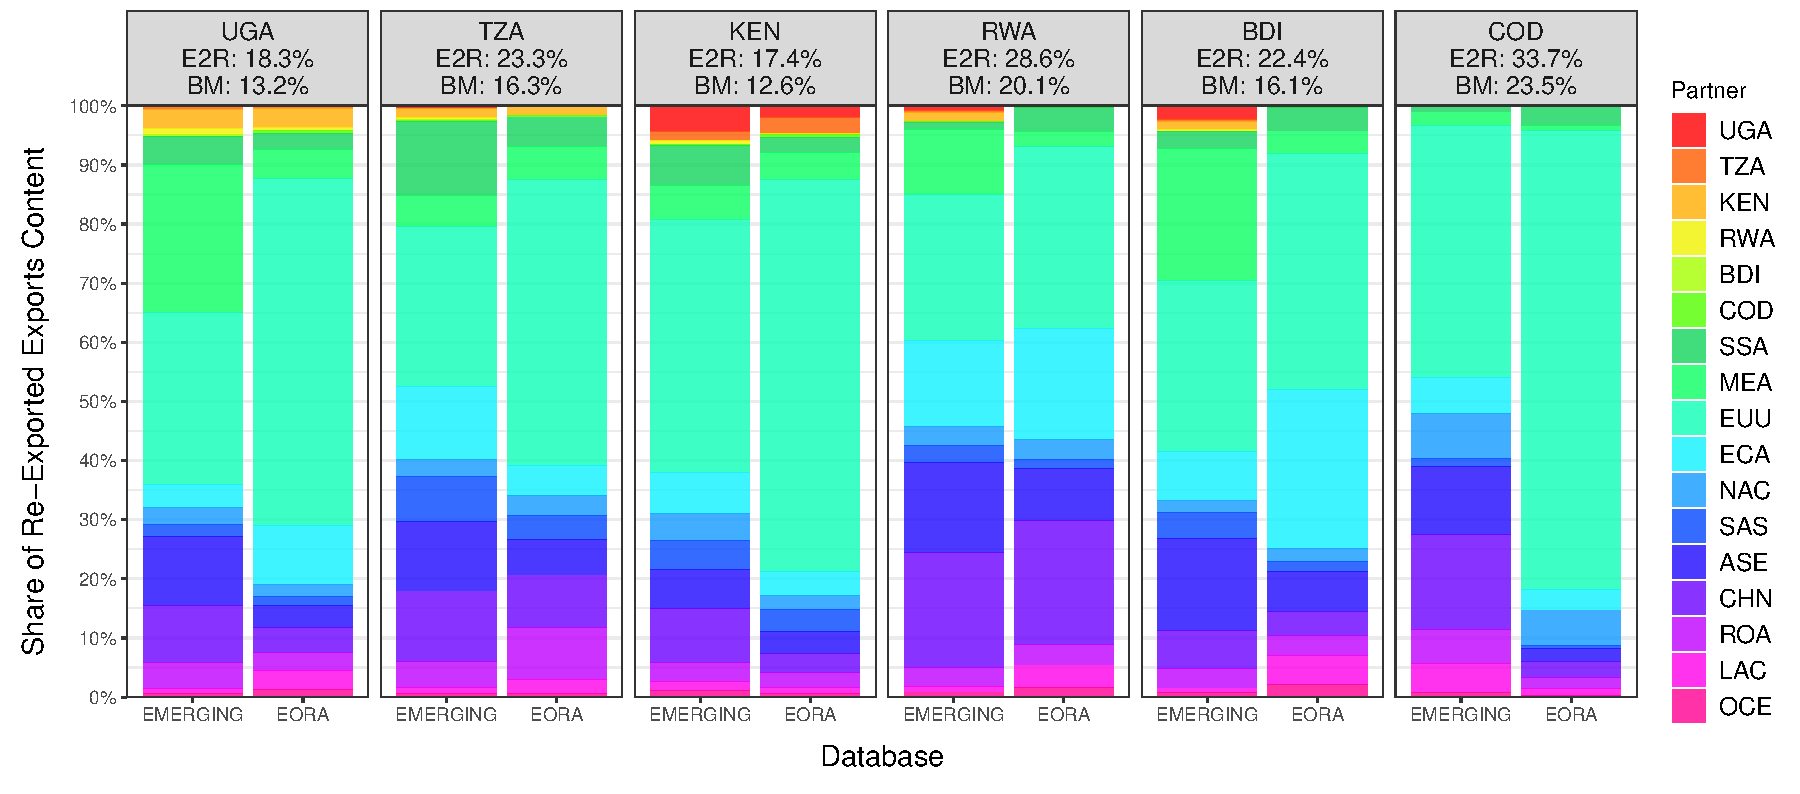
\includegraphics[width=1\textwidth]{"../Figures/REV/VS1_shares_ctry.pdf"} \\ %trim={<left> <lower> <right> <upper>}
\raggedright
\scriptsize
\vspace{-3mm}
\emph{Notes:} Figure shows a breakdown of forward GVC integration by GVC partner according to EM 2015-2019 averages. The classical VS1 measure of \citet{daudin2011produces} (Eq. \ref{eq:VS1}, also termed E2R) is used to determine each partners share in total VS1. The headers provide overall VS1 using both E2R and the corrected measure by \citet{borin2019measuring}. 
\end{figure}
\FloatBarrier

Table \ref{tab:EACVS1_sec} the shows the overall sector-level forward GVC participation similarly to Table \ref{tab:EACVB_sec} for backward GVC participation, and highlights considerable heterogeneity across EAC countries and sectors. In the EAC5 (Excl. Congo), around 21\% of gross exports in agriculture and manufactured products is re-exported VA as part of GVCs. 

% latex table generated in R 4.3.0 by xtable 1.8-4 package
% Fri Jan 12 12:32:02 2024
\begin{table}[h]  \vspace{-1mm}
\centering
\caption{\label{tab:EACVS1_sec}\textsc{EAC Forward GVC Participation: Sectoral Heterogeneity}}
\small{\textit{Average EMERGING 2015-2019 Re-Exported Content Share (VS1 following BM)}} \\
\vspace{1mm}
\begin{tabular}{lrrrrrrrrrr}
  \toprule
sector & UGA & TZA & KEN & RWA & BDI & COD & Mean & Median & EAC6 & EAC5 \\ 
  \midrule
AFF & 16.1 & 17.0 & 27.8 & 13.5 & 21.0 & 21.8 & 19.5 & 19.0 & 21.3 & 21.2\\ 
  MIN & 28.1 & 14.3 & 15.7 & 3.4 & 6.8 & 31.1 & 16.6 & 15.0 & 30.7 & 14.7\\ 
  FBE & 11.3 & 19.3 & 11.4 & 13.2 & 19.2 & 15.6 & 15.0 & 14.4 & 13.3 & 12.9\\ 
  MAN & 22.0 & 23.4 & 11.9 & 42.8 & 21.6 & 23.7 & 24.2 & 22.7 & 22.5 & 21.0\\ 
  SRV & 7.8 & 10.2 & 10.0 & 7.6 & 8.3 & 12.1 & 9.3 & 9.2 & 9.6 & 9.5\\
   \bottomrule \\ [-0.9em]
\multicolumn{11}{l}{\parbox{0.85\textwidth}{\scriptsize
\textit{Notes:} Table reports total forward GVC participation (VS1) following  \citet{borin2019measuring} using the EM 2015-2019 average in percentage terms. These shares are reported for each EAC6 country, and for the EAC6 and EAC5 as a whole, which includes re-exported VA by EAC members among each other. They are thus exort-weighted averages. The 'Mean' and 'Median' columns give unweighted EAC6 averages.}}
\end{tabular}
\vspace{-2mm}
\end{table}
\FloatBarrier

Since forward EAC GVC integration focuses on Uganda and Kenya, I also examine this link at the sector-level, using again the E2R measure available at the bilateral-sector level. In nominal terms, based on EMERGING 2015-19 averages, Kenya exports 81 million USD through Uganda, which amounted to 4.4\% of Kenyas VS1 and 0.76\% of Kenyas gross exports. 54\% of these 81 million are manufactured goods, 20\% are services, and 17\% agricultural products. Uganda on the other hand exports 30 million USD through Kenya, which amounts to 3.2\% of Ugandan VS1 and 0.58\% of Ugandan gross exports. Of these 30 million, 45\% are agricultural products, 22\% services, and 18\% manufacturing and 16\% processed foods and beverages. The links between these two countries account for the bulk of EAC forward GVC integration, summarized compactly by Table \ref{tab:EACVS1_ctry_sec}. Of particular interest in this table is the EAC share in sectoral VS1, which is high at 20.7\% for Kenyan manufactures, indicating that about 1/5th of re-exported VA in Kenyan manufacturing is accounted for by its EAC Partners. Other notable figures are the 41\%/29\% EAC shares in re-exported Rwandan/Kenyan mining exports, which are, however, very small in value. 

% latex table generated in R 4.3.0 by xtable 1.8-4 package
% Thu Jan 11 17:38:54 2024
\begin{table}[h!] \vspace{-1mm}
\centering
\caption{\label{tab:EACVS1_ctry_sec}\textsc{EAC Forward GVC Integration at the Sector Level}}
\small{\textit{Average EMERGING 2015-2019 Traditional VS1 Estimates \citep{daudin2011produces}  }} \\ % \citep{koopman2014tracing}
\vspace{1mm}
\resizebox{\textwidth}{!}{
\begin{tabular}{lrrrrrrrrrrrrr}
  \toprule
  & \multicolumn{5}{c}{VS1 (Re-Exported By EAC Partners)} & \multicolumn{3}{c}{Total + EAC Shares} & \multicolumn{5}{c}{EAC Share in Sectoral VS1} \\
Country & AFF & FBE & MAN & MIN & SRV & TOT & VS1 & EXP & AFF & FBE & MAN & MIN & SRV \\ 
  \midrule
UGA & 18.23 & 6.05 & 13.52 & 0.00 & 11.98 & 49.78 & 5.60 & 0.95 & 6.36 & 9.05 & 6.37 & 6.79 & 4.12 \\ 
  TZA & 11.06 & 9.20 & 12.40 & 1.15 & 17.64 & 51.45 & 2.80 & 0.61 & 3.44 & 5.89 & 3.03 & 8.91 & 1.91 \\ 
  KEN & 19.58 & 9.24 & 65.88 & 0.98 & 28.33 & 124.01 & 6.83 & 1.17 & 3.22 & 6.50 & 20.74 & 28.73 & 3.86 \\ 
  RWA & 3.63 & 3.08 & 3.39 & 0.00 & 3.59 & 13.69 & 2.86 & 0.80 & 13.98 & 12.99 & 1.21 & 41.04 & 2.27 \\ 
  BDI & 0.37 & 1.27 & 0.38 & 0.01 & 0.33 & 2.37 & 4.37 & 0.97 & 5.49 & 7.49 & 2.98 & 3.01 & 2.24 \\ 
  COD & 0.22 & 0.10 & 1.33 & 0.46 & 0.34 & 2.45 & 0.06 & 0.02 & 0.07 & 0.08 & 0.06 & 0.05 & 0.07 \\ 
   \bottomrule \\ [-0.9em]
\multicolumn{14}{l}{\parbox{1.05\textwidth}{\scriptsize
\textit{Notes:} VS1 is recorded in million USD, shares in percentag terms. Column 'TOTAL' gives total VS1 through EAC partners and columns 'VS1' and 'EXP' give the share of this in the countries total VS1 and gross exports, respectively.}}  \vspace{-1mm}
\end{tabular}
}
\end{table}
\FloatBarrier

To complete the picture, Figure \ref{fig:EACVS1_ctry_sec} shows the sector-level shares in forward GVC parters for the EAC5 (Excl. Congo). The EAC share is highest in mining at 13\%, but, Congo being excluded, mining VS1 comprises only 13 million USD, compared to 2.8/3 billion in AFF/FBE, 7.8 billion in manufacturing, and 5.6 billion in services re-exports. Of these the EAC has a share of 4\% in AFF, and 6.7\% in both FBE and MAN, indicating that manufacturing accounts for the bulk of GVC forward regional integration. The biggest forward GVC partner in all sectors remains the EU, at shares between 47\% for AFF and 16\% for MIN and MAN. 


\begin{figure}[h!] \vspace{-1mm}
\centering
\caption{\label{fig:EACVS1_ctry_sec}\textsc{EAC Forward GVC Participation: GVC Partners by Sector}}
\small{\textit{Based on Average EMERGING 2015-2019 EAC Exports (Excl. Congo)}} \\
\vspace{1mm}
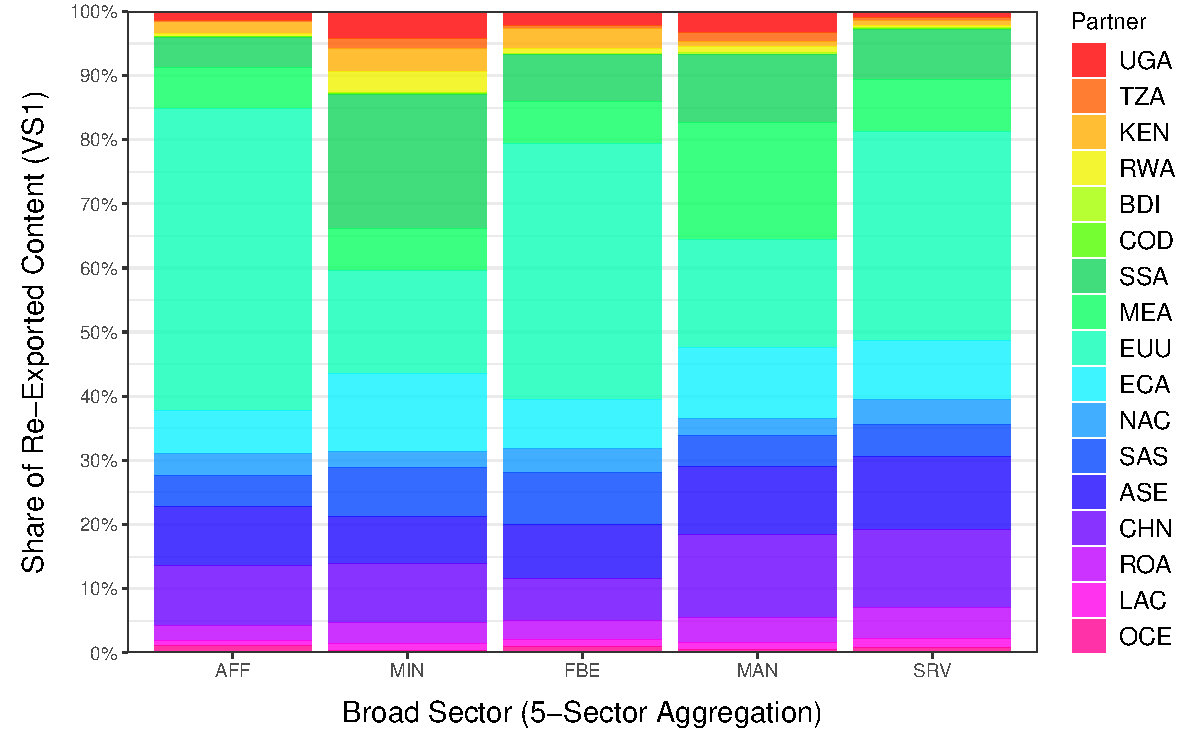
\includegraphics[width=0.7\textwidth]{"../Figures/REV/VS1_shares_sec_ctry.pdf"} \\ %trim={<left> <lower> <right> <upper>}
\raggedright
\scriptsize
\vspace{-1mm}
\emph{Notes:} Figure shows a sector-level breakdown of total EAC5 VS1 (E2R) by GVC partner using EM (2015-2019) averages. \\ \vspace{-3mm}
\end{figure}
\FloatBarrier

%Figure \ref{fig:EAC_E2R_ts} shows VS1 by exporting region for each EAC member country. It is between 10 and 25\% of gross exports for all EAC members, and similar to the level of VS in most EAC countries (Appendix Figure \ref{fig:VSag_ts} visualizes both measures over time). However, unlike VS, there is a clear downward trend in VS1 for all EAC members apart from Kenya. The literature (e.g. \citet{foster2015global}, \citet{Kummritz20161, Kummritz20162}) associates increased forward integration (VS1) into GVCs with productive upgrading. Figure \ref{fig:EAC_E2R_ts} thus points to a broad-based failure to upgrade production in the EAC. In terms of composition, most VS1 is exported by the EU, with a significant role for Asia, particularly China, but also the MEA and SSA regions. Kenya also exports around 1\% of gross Ugandan exports, and Tanzania and Uganda each export around 0.5\% of gross Kenyan Exports. Appendix Figure \ref{fig:EAC_E2R_ts_bar} further elicits the difference in shares between 2005 and 2015 in Figure \ref{fig:EAC_E2R_ts}, indicating that also inner-EAC VS1 decreased except in Kenya. 

%The following section develops dedicated metrics to better elicit patterns of EAC regional integration relative to EAC members overall GVC integration. % , the following section develops  
%Figure \ref{fig:VSag_ts} visualizes both measures over time. Uganda has very similar VS and VS1 ratios at 11-12\% of exports towards the end of 2015. The rise of VS in Tanzania, as already noted, is a statistical artifact of declining GDP and rising exports in the EORA data. Like Uganda, Tanzania appears to have experienced a slight decline in forward GVC participation down to 11\% of exports being re-exported in 2015. Kenya exhibits a stable development with VS of around 17\% and VS1 around 12.5\%. Rwanda experienced a stronger decrease in VS1 from initially 22.5\% down to 16\% in 2015. Burundi exhibits a relatively stable development with VS at 16\% and VS1 at 18\% in 2015. It is noteworthy that none of the EAC members significantly increased its forward integration (VS1) into GVCs, which the literature (e.g. \citet{foster2015global}, \citet{Kummritz20161, Kummritz20162}) associates with productive upgrading. %, congruent to the analysis if intermediate inputs in gross and VA terms in previo sections. 

%\begin{figure}[h!]
%\centering
%\caption{\label{fig:EAC_E2R_ts}\textsc{EAC Re-Exported Exports Shares (VS1)}}
%\includegraphics[width=1\textwidth, trim= {0 0 0 0}, clip]{"../Figures/E2R_shares_ag_ts_area".pdf} %trim={<left> <lower> <right> <upper>}
%\end{figure}
%\FloatBarrier




\subsection{Trends in EAC Regional Integration in Value-Added Terms}

Whereas overall EAC GVC integration appears relatively stable, with an increase in VS up to 2015 and heterogeneous developments thereafter, and gradual decline in VS1 in the more advanced EAC members, there may be more meaningful trends in regional integration relative to overall trade and GVC integration - as evident in gross trade flows. In this section I %develop measures to track regional integration both in VA terms through a new set of RVC indicators. 
% there may be regional developments not immediately apparent from standard indicators measuring overall GVC participation. This section, therefore, 
% In particular, I 
thus introduce four metrics to track EAC regional integration through VA in supply chains, relative to the overall GVC integration of member countries. The first metric is the share of foreign VA in a member's production/exports accounted for by its EAC partner states. It is computed as 
%
\begin{equation} \label{eq:VS_EAC}
\text{VS}_{uj}^{EAC} = \frac{1}{\text{VS}_{uj}}  \sum_{oi \in EAC,\ o \neq  u} \text{vb}_{oi, uj}   \ \ \forall\ uj \in EAC,
\end{equation} 
%
\noindent where VS$_{uj}$ is defined as in Eq. \ref{eq:VS}. VS$^{EAC}$ is thus a relative measure tracking the EAC share in VS, as shown also in Figure \ref{fig:EACVB_ctry}, such that the overall EAC VA share in domestic production can be computed as VS$_{uj}^{EAC} \times \text{VS}_{uj} \ \forall\ uj$. I define an analogous measure for VS1 as the proportion of domestic VA in re-exported exports exported by EAC partner states, as in Figure \ref{fig:EACVS1_ctry}. 
%
\begin{equation} \label{eq:VS1_EAC}
\text{VS1}_{oi}^{EAC} =  \sum_{uj \in EAC, u \neq  o} \text{vbe}_{oi, uj} \bigg/ \sum_{uj, u \neq  o} \text{vbe}_{oi, uj}\ \ \forall\ oi \in EAC.
\end{equation}
%
These two metrics effectively track the role of the EAC in forming the interaction of each member country with ROW in terms of backwards and forwards production and export linkages. They do, however, not account for the import side, i.e., the role of the EAC in providing goods and services to each member country relative to ROW. I thus compute two additional metrics to capture this aspect of regional integration. The first is the share of EAC VA in members imports, which I denote by VAI$^{EAC}$. Consider $E_u$ the vector of gross exports to EAC using country $u \in EAC$ from each country-sector\footnote{Since EORA does not record final demand by sector, I can only compute VAI$^{EAC}$ by receiving country. \vspace{-8mm}}. I then compute the VA origins of these exports to country $u$ as 
%
\begin{equation}
E_u^{VA} = \textbf{VB}E_u,
\end{equation}
%
\noindent where $E_u^{VA}$ denotes the vector, with elements $e_{oi, u}^{VA}$, of VA supplied by each country-sector ($oi$) in these imports of country $u$. From  $E_u^{VA}$, the share of EAC VA is easily computed as 
%
\begin{equation}
\text{VAI}_u^{EAC} = \sum_{oi \in EAC, o \neq u}  e_{oi, u}^{VA}  \bigg/ \sum_{oi, o \neq u}  e_{oi, u}^{VA}.  
\end{equation}
%
VAI$_u^{EAC}$ is thus a country-level measure of the VA by its EAC partners in its import mix, excluding any domestic VA in imports. This VA may include intermediates of exported goods. To single out the EAC share in imported consumption goods, I also consider only exports for final consumption. Let $FE_u$ be the final exports to country $u$ from each country-sector. Then $FE_u^{VA} = \textbf{VB}FE_u$ denotes these exports in VA terms, and I define
%
\begin{equation} \label{eq:VAFI_EAC}
\text{VAFI}_{u}^{EAC} = \sum_{oi \in EAC, o \neq u}  fe_{oi, u}^{VA}  \bigg/ \sum_{oi, o \neq u}  fe_{oi, u}^{VA}
\end{equation}
%
\noindent as the EAC VA share in final goods exported to a particular member $u$. I compute these metrics using the MRIO tables with reduced country dimension, except for $\text{VS1}_{oi}^{EAC}$ where I use the tables with reduced sectoral dimension. Figure \ref{fig:VAEACshares} plots all discussed metrics, and additionally fits a weighted linear trend, giving all observations a weight of 1, except for EMERGING 2010 obs. which receive a weight of 2 because no further data is observed until 2015, and EORA 2016-21 obs. receive a weight of 0.1 due to the stark structural break with the earlier series. 
%
%robust MM linear trend with 50\% breakdown point following \citet{koller2011sharpening} and \citet{robustbase}, which ignores outliers and structural breaks induced by updated EORA 2016-2021 tables. 
%
\begin{figure}[h!] \vspace{-3mm}
\centering
\caption{\label{fig:VAEACshares}\textsc{EAC5 VA Shares in Members VS, VS1, Imports and Final Imports}}
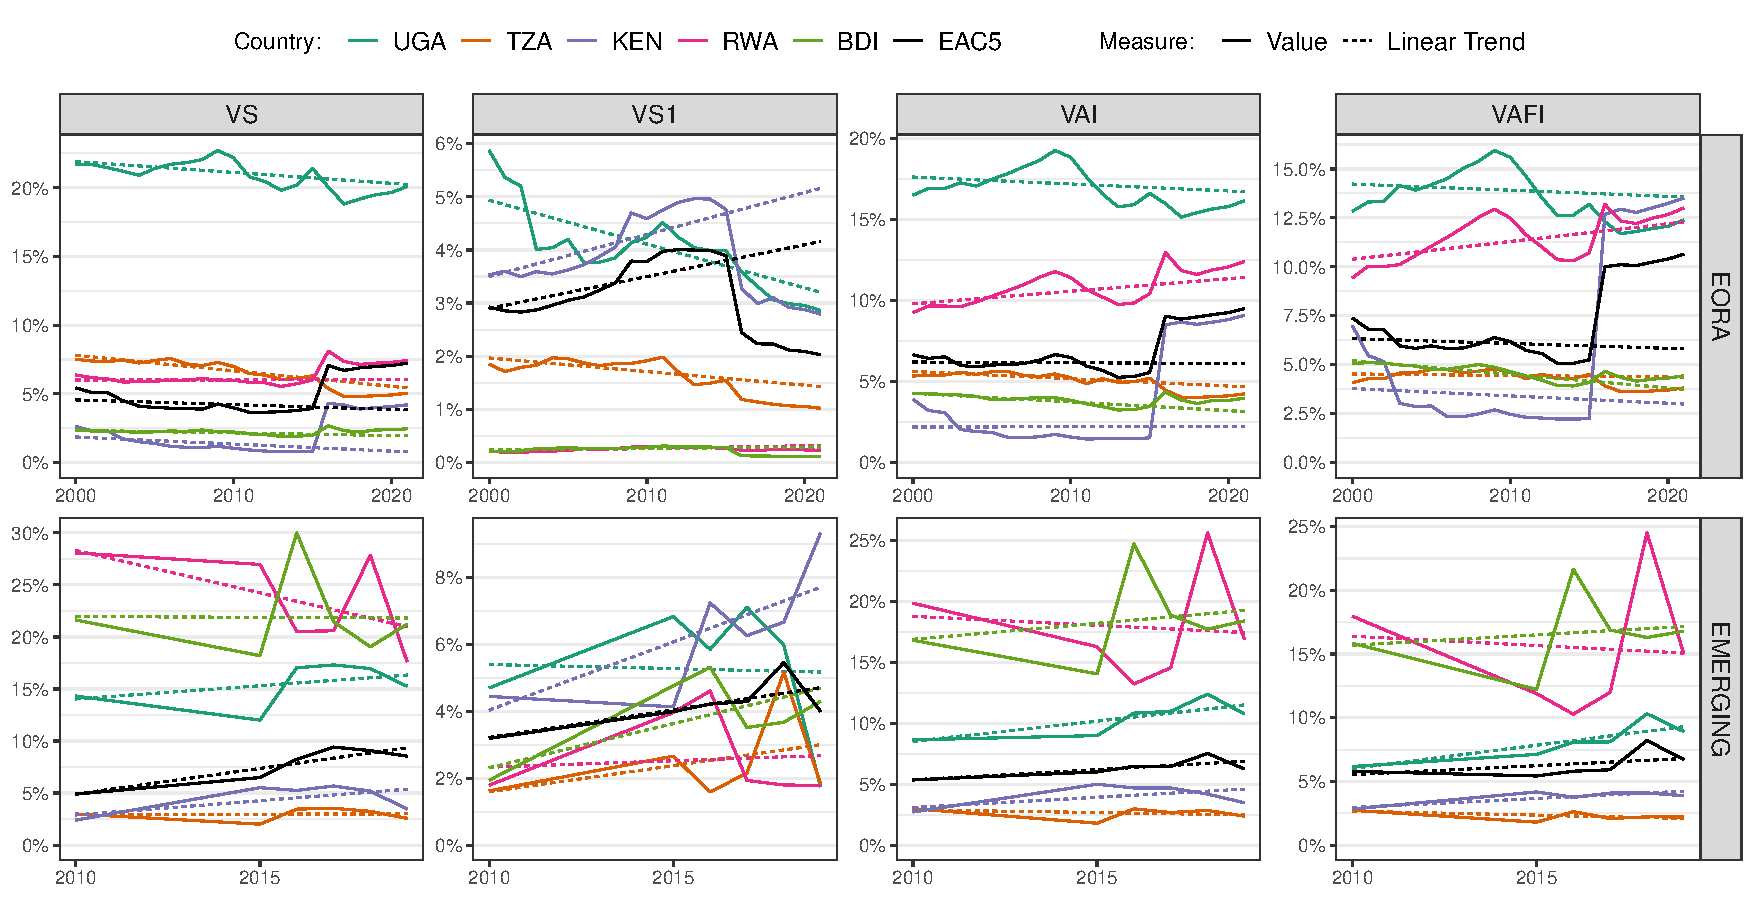
\includegraphics[width=1\textwidth, trim= {0 0 0 0}, clip]{"../Figures/REV/VA_EAC5_shares_ts.pdf"} \\ % "../Figures/VA_EAC_shares_ts".pdf
\raggedright
\scriptsize
\emph{Notes:} Figure shows regional EAC regional integration metrics follows Eqns. \ref{eq:VS_EAC}-\ref{eq:VAFI_EAC}, including a (weighted) linear trend. 
\end{figure}
\FloatBarrier
%
Both databases agree that EAC shares in members VS1 are substantially lower than in VS, VAI, and VAFI, but increased over the period, mainly driven by Kenya. They also agree that EAC forward linkages are driven by the larger economies, and smaller economies (Rwanda and Burundi) are more important in backward linkages (VS) and as importers of final goods (VAFI). Otherwise, there is not much agreement regarding the direction of the trend. To make Figure \ref{fig:VAEACshares} more intelligible, Figure \ref{fig:VAEACshares_bar} plots the slope coefficients. %As indicated, apart from Kenya's rising VS1 share with the EAC, and the resulting overall VS1 in crease in the EAC5 block, as well as a slight decrease in EAC share of Tanzanian imports (gross and final), and the fact that all of these slope estimates are small (less than 0.5 percentage points change per year), there is no common ground between the two databases at all regarding the evolution of EAC regional integration in VA terms. 
The more reliable EM database suggests that, with few exceptions, EAC regional integration in VA terms is increasing in most countries according to most measures. Considering the EAC5 as a whole, the coefficients suggest the the EAC share in EAC VS is increasing by 0.5 percentage points per year, and the EAC shares in EAC VS1, VAI, and VAFI are increasing at a slower rate of around 0.15 percentage points per year. These trends mildly contrast those from gross trade (Figure \ref{fig:GTEACshares}) indicating declining import shares. 
%
\begin{figure}[h!] \vspace{-5mm}
\centering
\caption{\label{fig:VAEACshares_bar}\textsc{Weighted Slope Estimates Measuring the Speed of Regional Integration}}
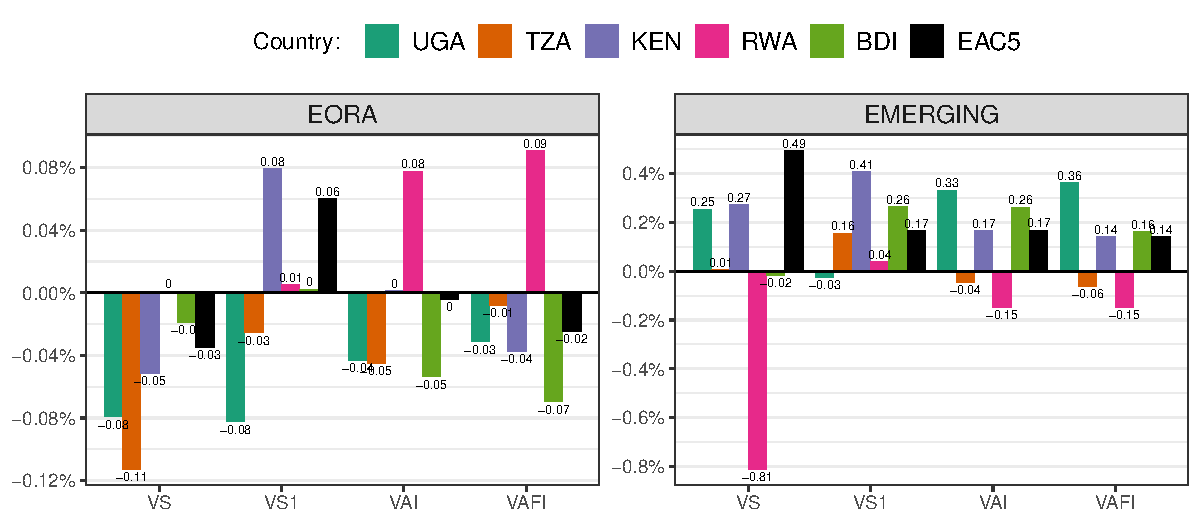
\includegraphics[width=1\textwidth, trim= {0 0 0 0}, clip]{"../Figures/REV/VA_EAC5_shares_slope_bar.pdf"} \\ % "../Figures/VA_EAC_shares_ts".pdf
\raggedright
\scriptsize
\emph{Notes:} Figure shows (weighted) linear slopes (dotted lines in Figure \ref{fig:VAEACshares}). In the estimation all obs. received a weight of $w=1$, except for EM 2010 ($w=2$) and EORA $>$ 2015 ($w=0.1$). These weights reflect data availability and quality.  
  \vspace{-1mm}
\end{figure}
\FloatBarrier
%
%Uganda and Tanzania follow very similar regional integration patterns, though at different levels. In Uganda, around 21\% of VS is accounted for by the EAC, whereas in Tanzania this was 6.3\% at the end of 2015. In Uganda, the EAC share of VS1 was close to 6\% end of 2015, vs 2\% in Tanzania. The EAC share in Ugandan imports (VAI) and final imports (VAFI) is in-between at 16.5\% and 14.5\% in 2015, respectively, whereas for Tanzania these shares were 5.2\% and 4.5\%. This suggests that both countries have stronger backward GVC linkages with the EAC, with EAC countries (Kenya in particular), supplying inputs into the production, whereas both countries play only a moderate role as suppliers of intermediates for export. Kenya exhibits the opposite pattern, with 7.4\% of Kenya's VS1 exported by its EAC partners, but only 0.9\% of VS coming from the EAC. The EAC share in VAFI at 2.3\% is also higher than VAI at 1.5\%, confirming that Kenya imports more final goods than intermediates from its EAC partners. \newline
%
%Rwanda and Burundi also follow a similar pattern of regional integration. In both countries, the final import share of the EAC is highest, at around 11\% in Rwanda and 4.3\% in Burundi in 2015. This is followed, with some distance, by the EAC share in VS, at 6.5\% in Rwanda and 2.2\% in Burundi. Both countries have a negligible supplier role for the EAC, with <1\% of their VS1 through EAC partners. South Sudan is also similar, with all measures below 1\% in 2015. \newline % indicating exclusion from RVCs. 
% 
% In summary, the progression of these indicators over time suggests that, except for Kenya's increasing role as a supplier of inputs for re-export by EAC members, EAC regional integration through value chains is stagnant or in decline, even when measured relative to an also mostly stagnant or declining overall level of GVC integration of the EAC member countries. 

As with gross trade, the weak aggregate signal indicates that there may be more substantial sectoral developments. I thus recompute all 4 indicators at the sector level using the EM database with full country dimension but only 5 broad sectors. Figure \ref{fig:VAEACshares_bar_sec} shows weighted linear slope estimates at the sector level (excluding mining), using again a weight of $2$ for 2010 estimates. 
%
\begin{figure}[h!] \vspace{-2mm}
\centering
\caption{\label{fig:VAEACshares_bar_sec}\textsc{Weighted Slope Estimates of Members Sectoral Integration Speed}}
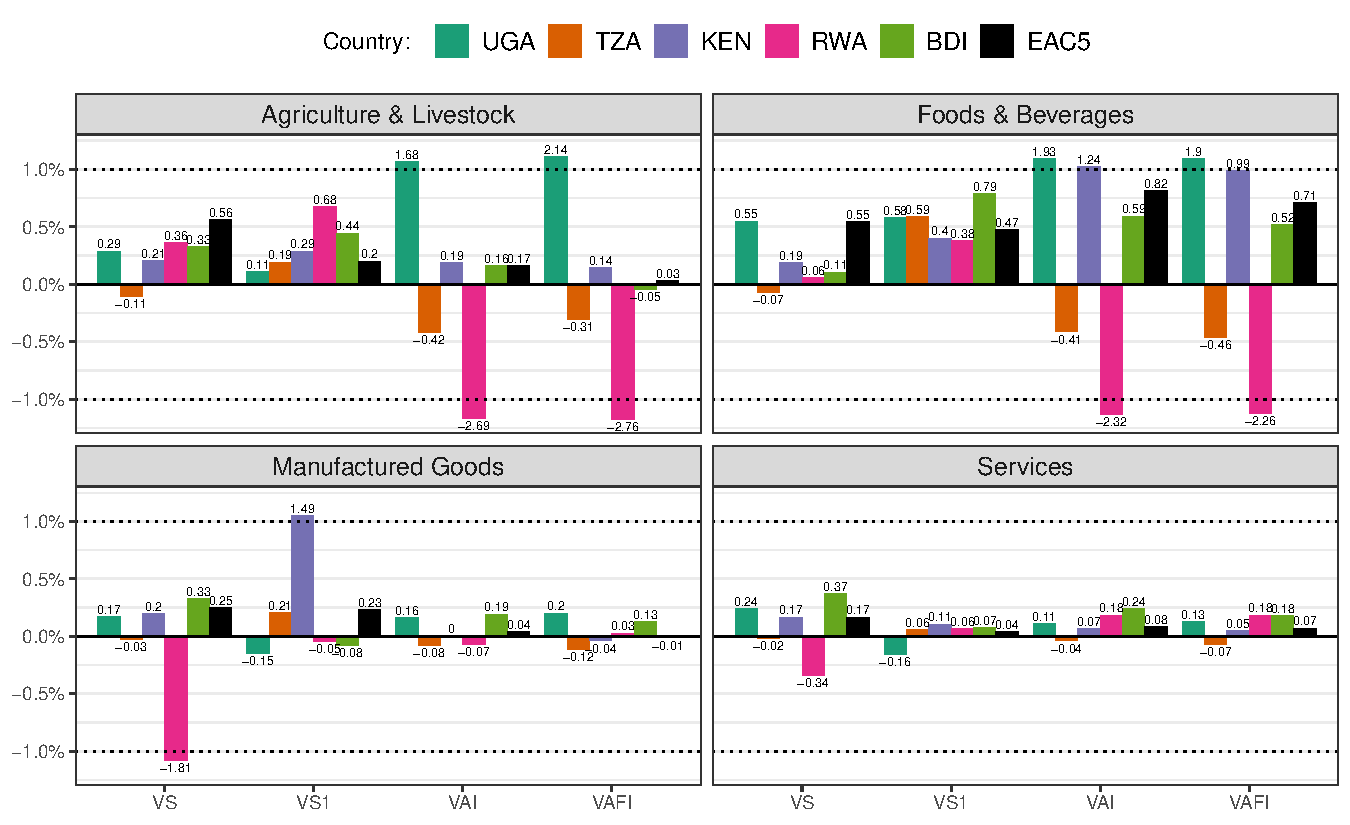
\includegraphics[width=1\textwidth, trim= {0 0 0 0}, clip]{"../Figures/REV/EM_VA_EAC5_shares_slope_bar_sec.pdf"} \\ % "../Figures/VA_EAC_shares_ts".pdf
\raggedright
\scriptsize
\emph{Notes:} Figure shows (weighted) linear slopes estimating the speed of regional integration (pp. per year) at the 5-sector level (excl. mining) based on EM (2010-2019). All obs. received a weight of $w=1$, except for EM 2010 ($w=2$).  
\vspace{-5mm}
\end{figure}
\FloatBarrier
%
The first thing to note in Figure \ref{fig:VAEACshares_bar_sec} is that regional integration in goods producing sectors proceeds substantially faster than in services. The aggregate pattern from Figure \ref{fig:VAEACshares_bar}, with faster integration through VS, is reflected in agriculture, manufacturing and services. The FBE sector on the other hand experienced stronger integration through forward linkages (VS1) and imports (VAI, VAFI), and overall greater integration speeds ($\geq 0.5$ pp. per year on all metrics). Uganda and Kenya are driving these developments. The regional integration in FBE through forward linkages (VS1) is also carried to almost equal shares by all 5 members, whereas the manufacturing expansion through forward linkages, proceeding at about half the speed as FBE, is driven almost completely by Kenya, with Tanzania contributing a little bit, and other members experiencing declining EAC shares in their manufacturing VS1. Overall the analysis of regional integration in VA terms complements Figures \ref{fig:EAC_ROW_Ratios_Sec} and \ref{fig:GTEACsharesSec}, indicating that there is some momentum on regional integration in agriculture and FBE, but equitable integration in manufacturing is difficult, and Kenya has strengthened its already favourable trading position through forward GVC linkages. 


\subsection{EAC Positioning in GVCs}

Following \citet{antras2012measuring, antras2022global}, a common measure of upstreamness $U_{oi} \ \in \ $ \textbf{u} is obtained by iterating forward the IO model in Eq. \ref{eq:io_model}, multiplying terms by the number of production stages needed to obtain them, and normalizing by gross output. In matrix notation: 
\begin{equation} \label{eq:upstreamness}
\textbf{u}\textbf{x} = \textbf{d} + 2\textbf{Ad} + 3\textbf{AAd} + 4\textbf{AAAd} + \cdots = (\textbf{I}-\textbf{A})^{-2}\textbf{d}.
\end{equation}
The index is, by definition, greater than 1, and \citet{antras2012measuring} state that it can be interpreted as the dollar amount by which the output of all country-sectors combined increases following a one dollar increase in the VA of sector $i$ in country $o$. Intuitively, it measures the distance of the production stage performed by sector $i$ in country $o$ to the finally demanded product (\textbf{d}).\footnote{An equivalent measure of downstreamness (\textbf{d}) can be computed measuring the distance to value-added instead of final demand \citep{antras2022global, miller2017output, mancini2023positioning}, but, for the sake of brevity, this is omitted. The simplest way of computing this index is as $\textbf{d}=\textbf{1}'\textbf{B}$, i.e., it is the column-sum of the Leontief inverse matrix \citep{miller2017output, antras2022global}. It can be interpreted as the total increase in gross output in the world economy that would be generated by a unit increase in final demand in the respective country-sector. At the world level \textbf{u} and \textbf{d} are identical and measure the length of GVCs \citep{mancini2023positioning}.} \citet{antras2012measuring} further find that $U$ is positively correlated with physical capital intensity and negatively correlated with skill intensity across US industries, and negatively correlated with rule of law, private credit to GDP, and education across a sample of OECD countries. Figure \ref{fig:EACUS_ag_ts} shows aggregate upstreamness for the EAC, calculated using the  regional MRIO tables with the full sector dimension, where sector-level $U_{oi}$ estimates were averaged using gross exports weights. \newline

% While upstreamness following Eq. \ref{eq:upstreamness} is the most widely used GVC positioning measure, 
\begin{figure}[h!]
\centering
\caption{\label{fig:EACUS_ag_ts}\textsc{Upstreamness Index for EAC Countries}}
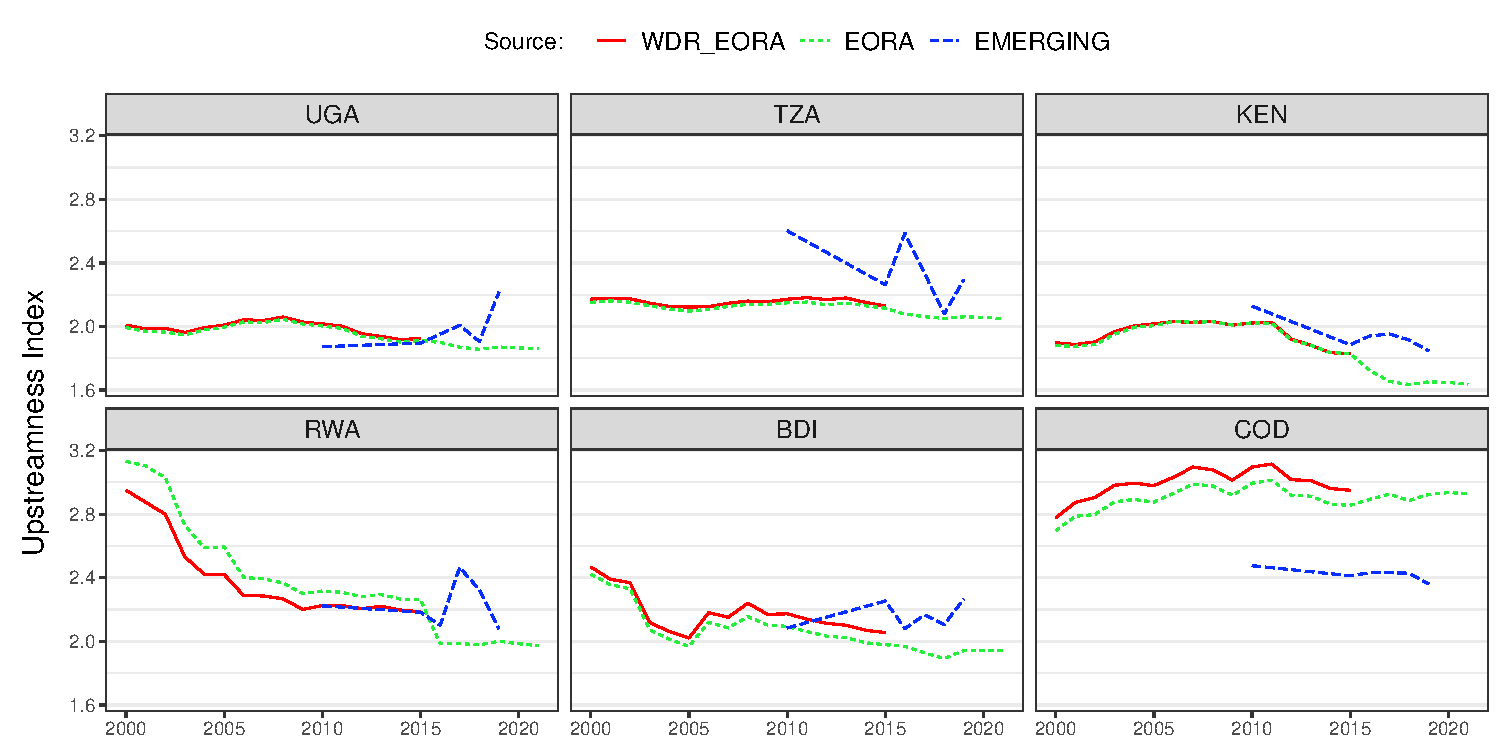
\includegraphics[width=1\textwidth, trim= {0 0 0 0}, clip]{"../Figures/REV/Upstreamness_ag_ts.pdf"} \\ %trim={<left> <lower> <right> <upper>}
\raggedright
\scriptsize
\emph{Notes:} Figure shows upstreamness index following \citet{antras2012measuring}, computed at the sector-level and averaged across sectors using sectoral gross exports as weights. The EORA and EM MRIOs have EAC + 11 regions and all sectors.  
\vspace{4mm}
\end{figure}
\FloatBarrier

% \todo[inline]{Compute position = upstreamness / downstreamness, and also create aggregate (exports weighted) EAC measure.}

%\todo[inline]{A final useful metric is to combine import and export upstreamness to compute the domestic length of the value chain. A positive gap indicates that exports are relatively more downstream (or “closer to final demand”) compared with imports  \citep{engel2016sacu}}

Figure \ref{fig:EACUS_ag_ts} shows that the computed $U$ index closely tracks the version computed by \citep{mancini2023positioning} using the full EORA 26 database and also performing an inventories adjustment following \citet{antras2018measurement}. The data suggest that Congo as a large commodity exporter is very upstream, and that all EAC members apart from Uganda and Burundi, where the EM estimates suggest a slight increase, moved more downstream since 2010. The most impressive development seems to have taken place in Rwanda during 2000-2010, but, since EORA does not have a Rwandan IO table, this trend must be interpreted with skepticism. \newline

To investigate developments at the sector level, I aggregate $U$ to broad sectors using export weights, combining all manufacturing sectors apart from FBE and all service sectors into broad categories. I also aggregate the time dimension over two intervals, 2010-2014 and 2015-2019, using the median to obtain a robust estimate. Table \ref{tab:U_BSEC} reports the results, including an estimate of the growth rate of $U$ between the two intervals and an export-weighted EAC5 average. \newline 

 The most upstream sector according to both databases is MIN, with $U>3$ signifying more than 3 production stages on average before final use. This is followed by MAN with $2 <U <3$ in most countries, FBE and primary AFF with $1.5 <U <2.5$ and SRV with $1 <U <2$. Except for SRV, this is broadly in line with the world average sectoral upstreamness pattern of, according to EM 2015-19, 3.32 (MIN), 2.86 (MAN), 2.62 (AFF), 2.25 (SRV) and 2.18 (FBE). The $U$ values of around 2/2.5 for EAC FBE/MAN indicates that these sectors are located at least one step before final use. For FBE where more than 90\% of VS1 is through non-EAC GVC partners (Figure \ref{fig:EACVS1_ctry_sec}), this implies that more processing steps could still be undertaken regionally to export products closer to final demand. The change between the two intervals yields a downstream shift in almost all country-sectors. This was particularly pronounced in AFF, MAN, and FBE, but also in SRV. The shift suggests that all production processes are moving closer to final demand. The world average growth rate in $U$ between these intervals according to EM was 3.3\% for AFF, 2.1\% for MIN, 0.85/0.82\% for FBE/MAN and -0.5\% for SRV, revealing that, except for SRV, EAC developments run against a global trend towards longer manufacturing GVCs \citep{antras2018measurement}. 

% latex table generated in R 4.3.0 by xtable 1.8-4 package
% Wed Jan 17 11:14:36 2024
\begin{table}[ht] \vspace{-2mm}
\centering
\caption{\label{tab:U_BSEC} EAC5 Trends in Upstreamness by Broad Sector (Aggregated)}
\vspace{2mm}
\resizebox{\textwidth}{!}{
\begin{tabular}{llrrrrrrrrrrrr}
  \toprule
  && \multicolumn{6}{c}{WDR Estimates using EORA 2015} & \multicolumn{6}{c}{EMERGING Estimates} \\
% Sector & Year & UGA & TZA & KEN & RWA & BDI & COD & UGA & TZA & KEN & RWA & BDI & COD \\ 
Sector & Year & UGA & TZA & KEN & RWA & BDI & EAC5 & UGA & TZA & KEN & RWA & BDI & EAC5 \\ 
  \midrule
% Same Estimates Including COD, excluding EAC5   
%  AFF & 2010-2014 & 2.17 & 2.38 & 1.56 & 2.36 & 3.49 & 2.78 & 1.86 & 1.88 & 2.30 & 1.80 & 1.98 & 1.82 \\ 
%  AFF & 2015-2019 & 2.13 & 2.36 & 1.49 & 2.35 & 3.33 & 2.76 & 1.91 & 1.84 & 1.83 & 1.28 & 1.77 & 1.65 \\ 
%  AFF & Growth Rate & -1.72 & -0.94 & -4.11 & -0.49 & -4.75 & -0.77 & 2.85 & -2.08 & -20.64 & -29.25 & -10.73 & -9.58 \\ 
%  MIN & 2010-2014 & 3.07 & 3.53 & 3.49 & 3.39 & 2.89 & 3.86 & 2.13 & 3.23 & 3.28 & 3.29 &  & 2.53 \\ 
%  MIN & 2015-2019 & 3.02 & 3.37 & 3.45 & 3.32 & 2.81 & 3.77 & 3.22 & 3.28 & 3.12 & 1.54 & 1.63 & 2.35 \\ 
%  MIN & Growth Rate & -1.62 & -4.46 & -1.40 & -2.23 & -2.81 & -2.27 & 51.20 & 1.56 & -5.02 & -53.27 &  & -7.25 \\ 
%  FBE & 2010-2014 & 1.47 & 1.58 & 1.41 & 1.39 & 1.50 & 1.70 & 2.23 & 2.04 & 2.34 & 2.57 & 2.32 & 1.92 \\ 
%  FBE & 2015-2019 & 1.44 & 1.57 & 1.34 & 1.36 & 1.45 & 1.68 & 2.15 & 2.12 & 2.18 & 2.35 & 2.41 & 1.81 \\ 
%  FBE & Growth Rate & -2.26 & -0.88 & -5.32 & -1.87 & -2.81 & -1.18 & -3.21 & 3.81 & -6.57 & -8.54 & 4.25 & -5.61 \\ 
%  MAN & 2010-2014 & 2.20 & 2.09 & 2.30 & 2.19 & 2.03 & 2.97 & 2.38 & 3.28 & 2.41 & 3.84 & 3.17 & 2.59 \\ 
%  MAN & 2015-2019 & 2.14 & 2.06 & 2.18 & 2.15 & 1.97 & 2.92 & 2.47 & 2.89 & 2.24 & 3.16 & 2.73 & 2.52 \\ 
%  MAN & Growth Rate & -2.62 & -1.57 & -5.34 & -1.68 & -3.15 & -1.84 & 3.81 & -11.79 & -7.11 & -17.74 & -13.96 & -2.58 \\ 
%  SRV & 2010-2014 & 1.73 & 1.89 & 1.77 & 1.70 & 1.79 & 2.29 & 1.35 & 2.19 & 1.83 & 1.40 & 1.47 & 1.62 \\ 
%  SRV & 2015-2019 & 1.70 & 1.85 & 1.64 & 1.67 & 1.74 & 2.25 & 1.52 & 2.09 & 1.65 & 1.61 & 1.41 & 1.61 \\ 
%  SRV & Growth Rate & -1.40 & -1.89 & -7.02 & -1.78 & -2.85 & -1.49 & 12.27 & -4.84 & -9.75 & 15.11 & -4.01 & -0.64 \\ 
% Estimates with EAC5, excluding COD: 
  AFF & 2010-2014 & 2.17 & 2.38 & 1.56 & 2.36 & 3.49 & 1.81 & 1.86 & 1.88 & 2.30 & 1.80 & 1.98 & 2.09 \\ 
  AFF & 2015-2019 & 2.13 & 2.36 & 1.49 & 2.35 & 3.33 & 1.76 & 1.91 & 1.84 & 1.83 & 1.28 & 1.77 & 1.84 \\ 
  AFF & Growth Rate & -1.72 & -0.94 & -4.11 & -0.49 & -4.75 & -2.68 & 2.85 & -2.08 & -20.64 & -29.25 & -10.73 & -12.06 \\ 
  MIN & 2010-2014 & 3.07 & 3.53 & 3.49 & 3.39 & 2.89 & 3.48 & 2.13 & 3.23 & 3.28 & 3.29 &  & 3.25 \\ 
  MIN & 2015-2019 & 3.02 & 3.37 & 3.45 & 3.32 & 2.81 & 3.41 & 3.22 & 3.28 & 3.12 & 1.54 & 1.63 & 3.17 \\ 
  MIN & Growth Rate & -1.62 & -4.46 & -1.40 & -2.23 & -2.81 & -2.08 & 51.20 & 1.56 & -5.02 & -53.27 &  & -2.44 \\ 
  FBE & 2010-2014 & 1.47 & 1.58 & 1.41 & 1.39 & 1.50 & 1.45 & 2.23 & 2.04 & 2.34 & 2.57 & 2.32 & 2.26 \\ 
  FBE & 2015-2019 & 1.44 & 1.57 & 1.34 & 1.36 & 1.45 & 1.38 & 2.15 & 2.12 & 2.18 & 2.35 & 2.41 & 2.13 \\ 
  FBE & Growth Rate & -2.26 & -0.88 & -5.32 & -1.87 & -2.81 & -4.37 & -3.21 & 3.81 & -6.57 & -8.54 & 4.25 & -5.59 \\ 
  MAN & 2010-2014 & 2.20 & 2.09 & 2.30 & 2.19 & 2.03 & 2.25 & 2.38 & 3.28 & 2.41 & 3.84 & 3.17 & 2.89 \\ 
  MAN & 2015-2019 & 2.14 & 2.06 & 2.18 & 2.15 & 1.97 & 2.15 & 2.47 & 2.89 & 2.24 & 3.16 & 2.73 & 2.63 \\ 
  MAN & Growth Rate & -2.62 & -1.57 & -5.34 & -1.68 & -3.15 & -4.42 & 3.81 & -11.79 & -7.11 & -17.74 & -13.96 & -9.02 \\ 
  SRV & 2010-2014 & 1.73 & 1.89 & 1.77 & 1.70 & 1.79 & 1.78 & 1.35 & 2.19 & 1.83 & 1.40 & 1.47 & 1.82 \\ 
  SRV & 2015-2019 & 1.70 & 1.85 & 1.64 & 1.67 & 1.74 & 1.69 & 1.52 & 2.09 & 1.65 & 1.61 & 1.41 & 1.77 \\ 
  SRV & Growth Rate & -1.40 & -1.89 & -7.02 & -1.78 & -2.85 & -4.82 & 12.27 & -4.84 & -9.75 & 15.11 & -4.01 & -2.66 \\ 
   \bottomrule \\ [-0.9em]
\multicolumn{14}{l}{\parbox{1.24\textwidth}{\scriptsize
\textit{Notes:} Table shows median in upstreamness ($U$) following \citet{antras2012measuring} across 2010-14 and 2015-19, and the growth rate in percentage terms between these medians. MAN and SRV are broad categories combining sectors TEX-MAN and EGW-PAO in Table \ref{tab:sec}, respectively, via an export weighted average. The EAC5 is an export weighted average across the 5 countries (excl. COD) computed annually before taking the median.  }}
\end{tabular}
}
\end{table}
\FloatBarrier

For all sectors apart from MAN and SRV this appears to be good news, indicating that exports are closer to final demand and more local value is added. For MAN this suggests a shift towards processing trade, which is generally not associated with industrial upgrading. The effect of SRV moving more downstream is unclear and depends very much on the type of service. For transport/tourism (TRA), a downstream shift posits more local value addition, whereas for telecommunications (PTE) and financial intermediation (FIB), downstream shifts might signify insufficient quality of these services to be used as intermediates in more complicated production processes. EAC data on these sectors are likely of questionable quality, yet, a brief disaggregated appraisal using EM yields, notably, a 28\% upstream/downstream shifts in FIB in Rwanda/Tanzania (EAC5 average is 5.3\% downstream), a 9.5/5.9\% downstream shift in PTE in Kenya/Rwanda (EAC5 average is 3\% downstream) and a 10.2/7.4\% downstream shift in TRA in Kenya/Burundi, whereas other EAC members saw a slight upstream shift (EAC5 average is 1.4\% downstream). 


\subsection{(New) Revealed Comparative Advantage}

In international trade, including GVC-related trade, competitiveness is related to the concept of comparative advantage\footnote{A widely accepted theory of international trade developed by David Ricardo in 1817 stipulating that countries specialize in sectors where their productivity relative to the international average is greatest.}. 
A popular way to empirically measure Ricardo's concept of comparative advantage is \citet{balassa1965trade}'s measure of revealed comparative advantage, defined as the share of a sector in gross country exports, divided by the share of that sector in gross world exports
%
\begin{equation}
\text{RCA}_{oi} = \frac{E_{oi}}{\sum_i E_{oi}} \Bigg/ \frac{\sum_j E_{ji}}{\sum_{ji} E_{ji}}.
\end{equation}
%
$\text{RCA}_{oi}>1$ signifies a revealed comparative advantage of country $o$ in sector $i$. The traditional index based on gross exports however does not account for GVCs and double counting in exports. \citet{koopman2014tracing} therefore propose a new index based on the domestic VA in gross exports (DVA). \citet{borin2019measuring} show that the decomposition of \citet{koopman2014tracing} is inexact in allocating domestic VA and foreign double counted items.%\footnote{In particular: "their classification does not properly allocate the domestic value-added in exports between the part eventually absorbed by direct importers and the part absorbed in third markets, and  a portion of the foreign content of exports is erroneously classified as 'double counted' whereas it should be allocated to the 'foreign value-added'." \citep{borin2019measuring}}. 
Appendix Figure \ref{fig:KWW} shows the refined breakdown following \citet{borin2019measuring}, and Figure \ref{fig:KWW_fill_ts} plots the decomposition of gross exports for each of the EAC members.\footnote{To connect this to the aggregate measures of GVC integration VS and VS1 discussed so far: VS, the share of FVA in gross exports, is the sum of FVA and FDC, whereas VS1 is the sum of NDAVAX, REF and DDC. \vspace{-5mm}} DVA is the sum of DAVAX, NDAVAX and REF. According to EM 2015-19, in the average EAC member DAVAX accounts for 71\% of gross exports, NDAVAX for 12\%, FVA for 14\% and FDC for 3\%. REF and DDC are close to 0 in all EAC countries, implying that the GVCs these countries engage in are relatively short. Thus, in the EAC, DVA $\approx$ E $-$ VS, yielding an average 17\% downward adjustment of gross exports. This may appear small, but, as Table \ref{tab:EACVB_sec} shows, manufacturing sectors have higher VS of up to 50\%. \newline
 
For comparison, I compute both classical RCA using gross exports (GX) and NRCA using DVA in exports (VAX), based on all available databases, including BACI (only available for goods producing sectors) and the WDR 2020 GVC indicators based on EORA 2015. Figure \ref{fig:NRCA} shows median (N)RCA estimates across years 2010-19 for the EAC5. 
%
\begin{figure}[h!] %\vspace{-2mm}
\centering
\caption{\label{fig:NRCA}\textsc{(New) Revealed Comparative Advantage: 2010-19 Median}}
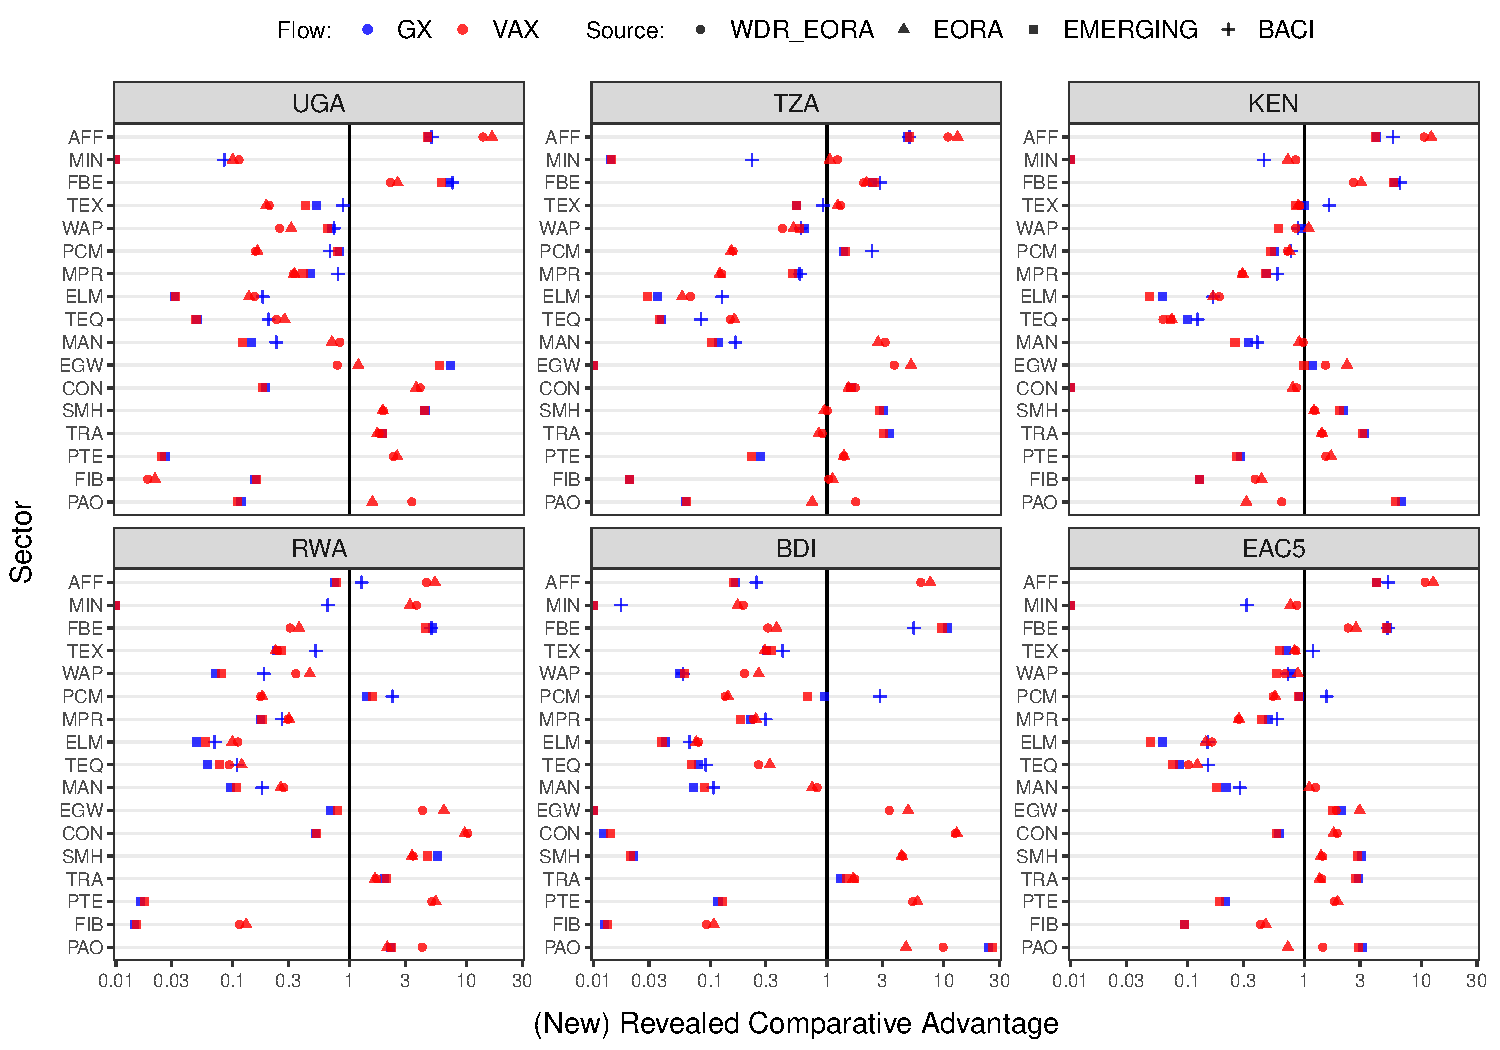
\includegraphics[width=1\textwidth]{"../Figures/REV/NRCA_EAC5_ALL.pdf"} % trim={<left> <lower> <right> <upper>}
\raggedright
\scriptsize
\emph{Notes:} Figure shows median 2010-19 (N)RCA indices based on DVA/gross exports according to different databases. DVA is computed following \citet{borin2019measuring}. Appendix Table \ref{tab:NRCA} contains the values and Table \ref{tab:NRCA_corr} their correlations. To not overcrowd the figure, GX-based estimates using (WDR\_)EORA are not shown. 
\end{figure}
\FloatBarrier
%
Appendix Tables \ref{tab:NRCA} and \ref{tab:NRCA_corr} contains the corresponding values and correlations among different estimates, %Table  further reports pairwise Pearson's correlations of these median estimates. 
reassuringly indicating that all RCA measures are correlated. Whereas EORA based estimates have a correlation of around 0.57 with the BACI estimates, EM estimates have a strong correlation of 0.93, confirming that these IO tables are very close to official trade data. In all IO tables RCA and NRCA estimates are also highly correlated ($r > 0.96$), suggesting that the foreign content shares in exported good within a sector are quite similar across different countries. \newline

All estimates show that the EAC5 as a whole, and, according to EM/BACI, also all the 5 countries individually, have a succinct (N)RCA in agriculture and food processing of, according to the EM NCRA estimates 4.17 (AFF) and 5.01 (FBE). Similarly, all countries have a sizeable disadvantage in all core manufacturing sectors except for textiles and petrochemicals. Especially electrical machinery (EML: 0.05) and transport equipment (TEQ: 0.08), core drivers of GVC expansion according to the WDR, have a strong revealed disadvantage. On the services side, all members have a (N)RCA in transport (and travel) services (TRA: 2.77), which is particularly strong in Kenya (3.12) and Tanzania (3.02), and all members apart from Burundi have a (N)RCA in sales, maintenance, and hotels (SMH: 2.84), particularly Uganda (4.36) and Rwanda (4.64). Furthermore, Uganda with its powerful dams, has a large (N)RCA in exporting electricity (5.87). EAC members thus exhibit similar patterns of revealed comparative advantage in agriculture, food processing and tourism, and a disadvantage in core manufacturing sectors. This is constitutive to forming a common trade block, supported by a monetary union as planned, and deepening regional tourism and food processing value chains to ensure that regional VA is maximized. Yet comparing the EAC with ROW masks rivalries and differences in (N)RCA between member countries. 

% \todo[inline]{Changes !!}

%\begin{figure}[h!]
%\centering
%\caption{\label{fig:NRCA}\textsc{New Revealed Comparative Advantage}}
%\includegraphics[width=1\textwidth, trim= {0 0 0 0}, clip]{"../Figures/NRCA_fl".pdf} %trim={<left> <lower> <right> <upper>}
%\end{figure}
%\FloatBarrier

% All EAC members have a NRCA in agriculture and fishing, which is higher than 10 for agriculture in Uganda, Tanzania, and Kenya, and a comparative disadvantage in core manufacturing sectors such as petrochemicals, metal products, and electrical machinery. On the services side, all members have NRCA in accommodation and food services (e.g. tourism). The remaining sectors show more heterogeneity across EAC countries, where Kenya appears to be different from the other countries. In Uganda, Tanzania, Rwanda, Burundi, and South Sudan activities of private households (self-employment) and maintenance and repair activities have strong NRCA, whereas in Kenya both appear to have a comparative disadvantage. It is also noteworthy that Uganda, Kenya, and to a lesser extent Tanzania have a comparative advantage in foods and beverages. \newline
%
%To better analyze changes in NRCA over time, Appendix Figure \ref{fig:NRCA_growth} shows the annualized growth rate in NRCA over the 2005-2015 period. NRCA has not changed much in agriculture, with minor annual gains or losses within the [-2\%, 2\%] range. All EAC members seem to have gained NRCA in fishing, particularly Uganda and Tanzania with gains of 2.2\% and 5.3\%, respectively. Also, all EAC members have lost NRCA in mining, especially Uganda. All EAC countries have gained NRCA in re-exporting goods. In other sectors, developments are rather heterogeneous. Uganda for example appears to have gained NRCA in exporting transport equipment by around 5.1\% annually, whereas Rwanda lost NRCA in the same sector by -4.1\% annually. Notably, Kenya records slight gains in NRCA in all core manufacturing sectors, whereas developments in other EAC countries are much more heterogeneous and wholly negative in Burundi.



\subsection{NRCA Relative to the EAC and in Inner-EAC Trade}

To uncover these differences, I also compute (N)RCA relative to the EAC, as the share of a sector in country exports to the share of the sector in EAC exports. Furthermore, regional trading itself reveals comparative advantages that can either foster or block deeper RVCs. Thus I also compute (N)RCA of each member relative to the regional trade mix. Figure \ref{fig:EAC_NRCA} presents both estimates, and Appendix Table \ref{tab:EAC_NRCA} the corresponding values. 

\begin{figure}[h!]
\centering
\caption{\label{fig:EAC_NRCA}\textsc{NRCA Relative to EAC5}}
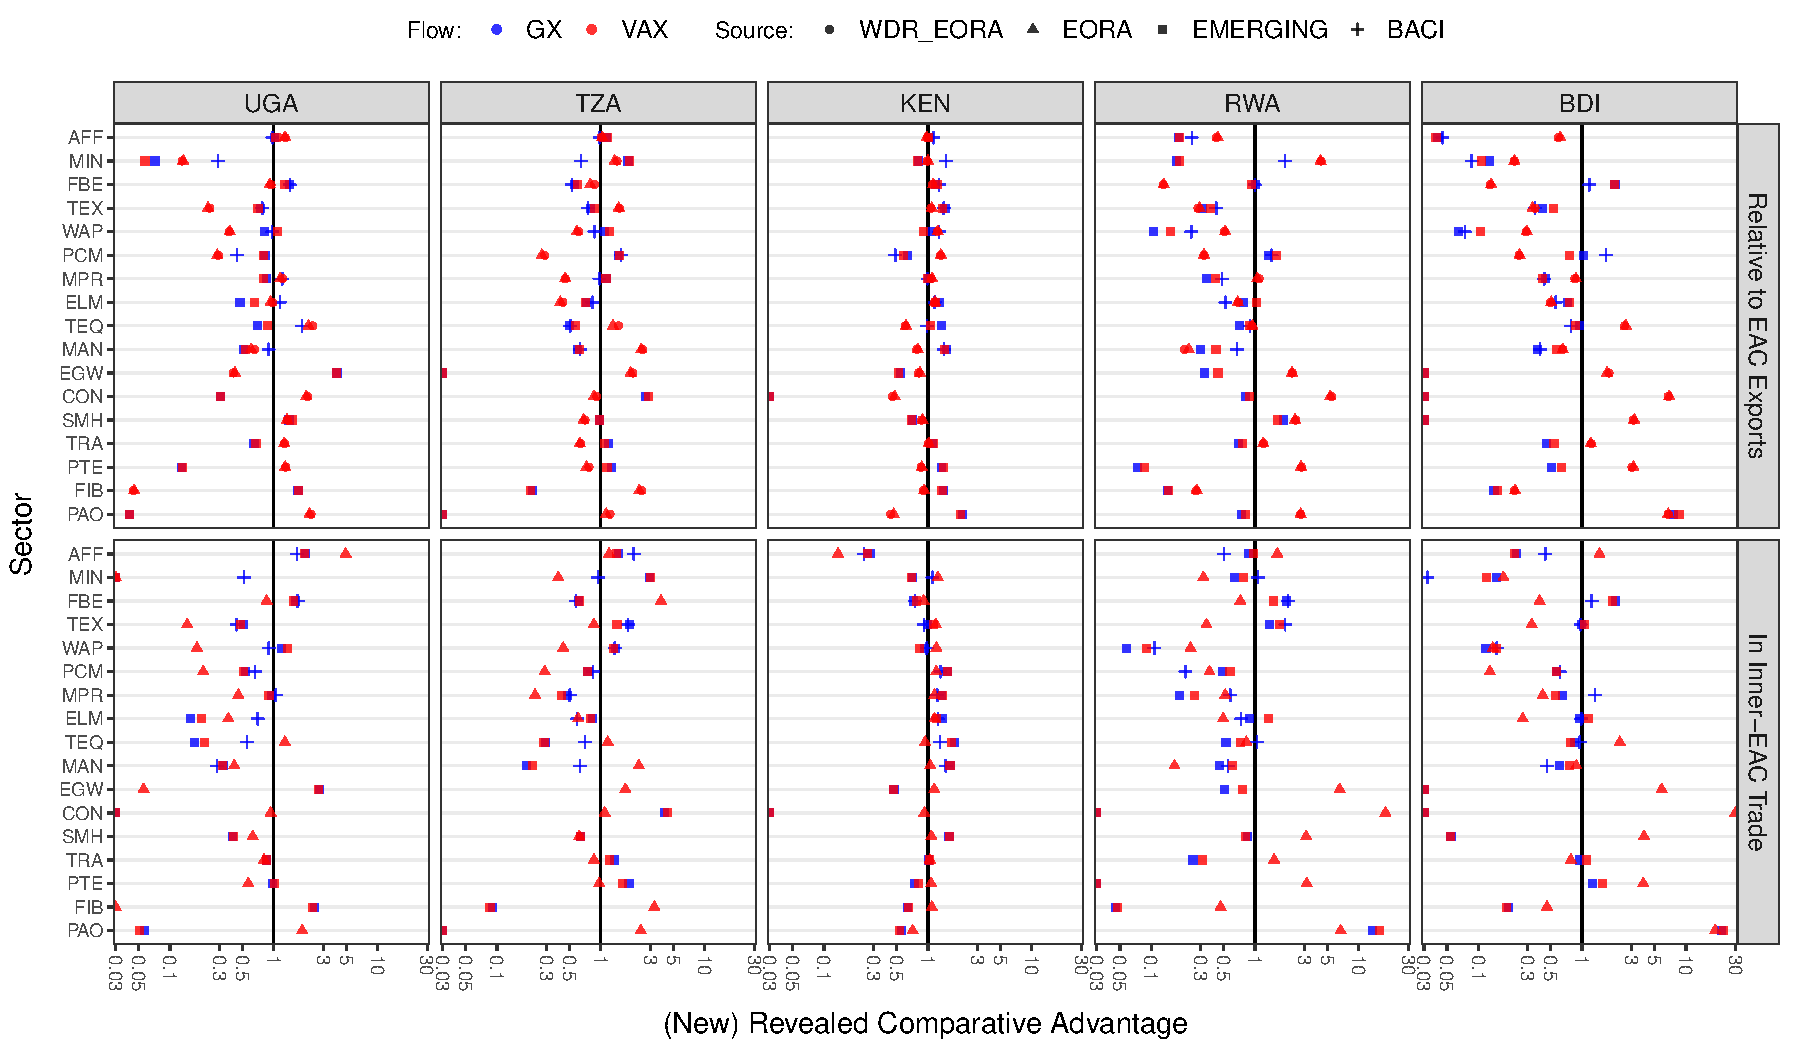
\includegraphics[width=1\textwidth]{"../Figures/REV/EAC_NRCA_EAC5_ALL.pdf"} %trim={<left> <lower> <right> <upper>}
\raggedright
\scriptsize
\emph{Notes:} Figure shows median 2010-19 (N)RCA indices based on DVA/gross exports according to different databases, calculated w.r.t. EAC5 exports (top panel) and w.r.t. total inner EAC5 trade (bottom panel). DVA is computed following \citet{borin2019measuring}. Appendix Table \ref{tab:EAC_NRCA} contains the corresponding values. To not overcrowd the figure, GX-based estimates using (WDR\_)EORA are not shown.
\end{figure}
\FloatBarrier
%\begin{figure}[h!]
%\centering
%\caption{\label{fig:NRCA_EAC}\textsc{NRCA Relative to EAC}}
%\includegraphics[width=1\textwidth, trim= {0 0 0 0}, clip]{"../Figures/NRCA_EAC_fl".pdf} %trim={<left> <lower> <right> <upper>}
%% \vspace{-1cm}
%\end{figure}
%\FloatBarrier

The estimates unveil that relative to other EAC members, Uganda, Tanzania, and Kenya, have a slight (1-1.2) (N)RCA in agriculture, and Uganda, Kenya, and Burundi have a (N)RCA in FBE of (1.2-1.5). In inner-EAC trade, Kenya's (N)RCA drops to 0.26/0.78 in AFF/FBE in VAX terms, whereas Uganda's rises to 2/1.5, reflecting its stronger regional supplier role. Rwanda has a (N)RCA in mining, but this is not reflected in inner-EAC trade. Kenya has a slight comparative advantage in manufacturing sectors, including TEX, MPR, ELM, TEQ, and other manufactures (MAN). Exempting TEX, and including PCM, these estimates are even higher in inner-EAC trade, but all in the range between 1 and 2, and thus significantly lower than with ROW. Tanzania also has a (N)RCA in PCM according to both denomination. As mentioned earlier, Kenya, and, to a lesser extent, Tanzania, also have a slight (N)RCA in TRA (1-1.2), both relative to the EAC and revealed in inner-EAC trade, and Uganda has a large (N)RCA in EGW (4-5). \newline
% , and Kenya in core manufacturing sectors such as wood and paper, petrochemicals, metal products, and electrical machinery. %In addition, it appears that Rwanda and Burundi, and to a weaker extent Uganda, have a comparative advantage in construction, maintenance and repairs, wholesale and retail trade, whereas Tanzania appears to have a comparative advantage in other manufacturing, recycling, and financial and business services. 
% Other sectors are more heterogeneous. 
% NRCA relative to the EAC is relatively stable since 2005, Appendix Figure \ref{fig:NRCA_EAC_growth} shows growth rates. %without major shifts within or across sectors between 2005 and 2015. 

The trading patterns of different members in both gross and VA terms thus reveal differences in comparative advantage, but these are, with few exceptions such as Ugandan EGW, between 0.5 and 2, and thus moderate in size. It may however still require policy action to overcome these differences and foster more horizontal RVC's in critical sectors such as FBE and tourism (TRA). 

\subsection{Trends in (N)RCA}

A final question regards the direction and speed of shifts in RCA, both overall and inside the EAC. To measure this, I only use gross trade from BACI and DVA from EM to compute (N)RCA medians over two periods: 2006-2010 and 2015-2019. I then compute the growth rate and report it in Figure \ref{fig:NRCA_GR}. Appendix Figure \ref{fig:NRCA_Diff} shows estimates for both periods, and Table \ref{tab:NRCA_Diff} holds all values. 

\begin{figure}[h!]
\centering
\caption{\label{fig:NRCA_GR}\textsc{Growth of (N)RCA Between 2006-2010 and 2015-2019 (Medians)}}
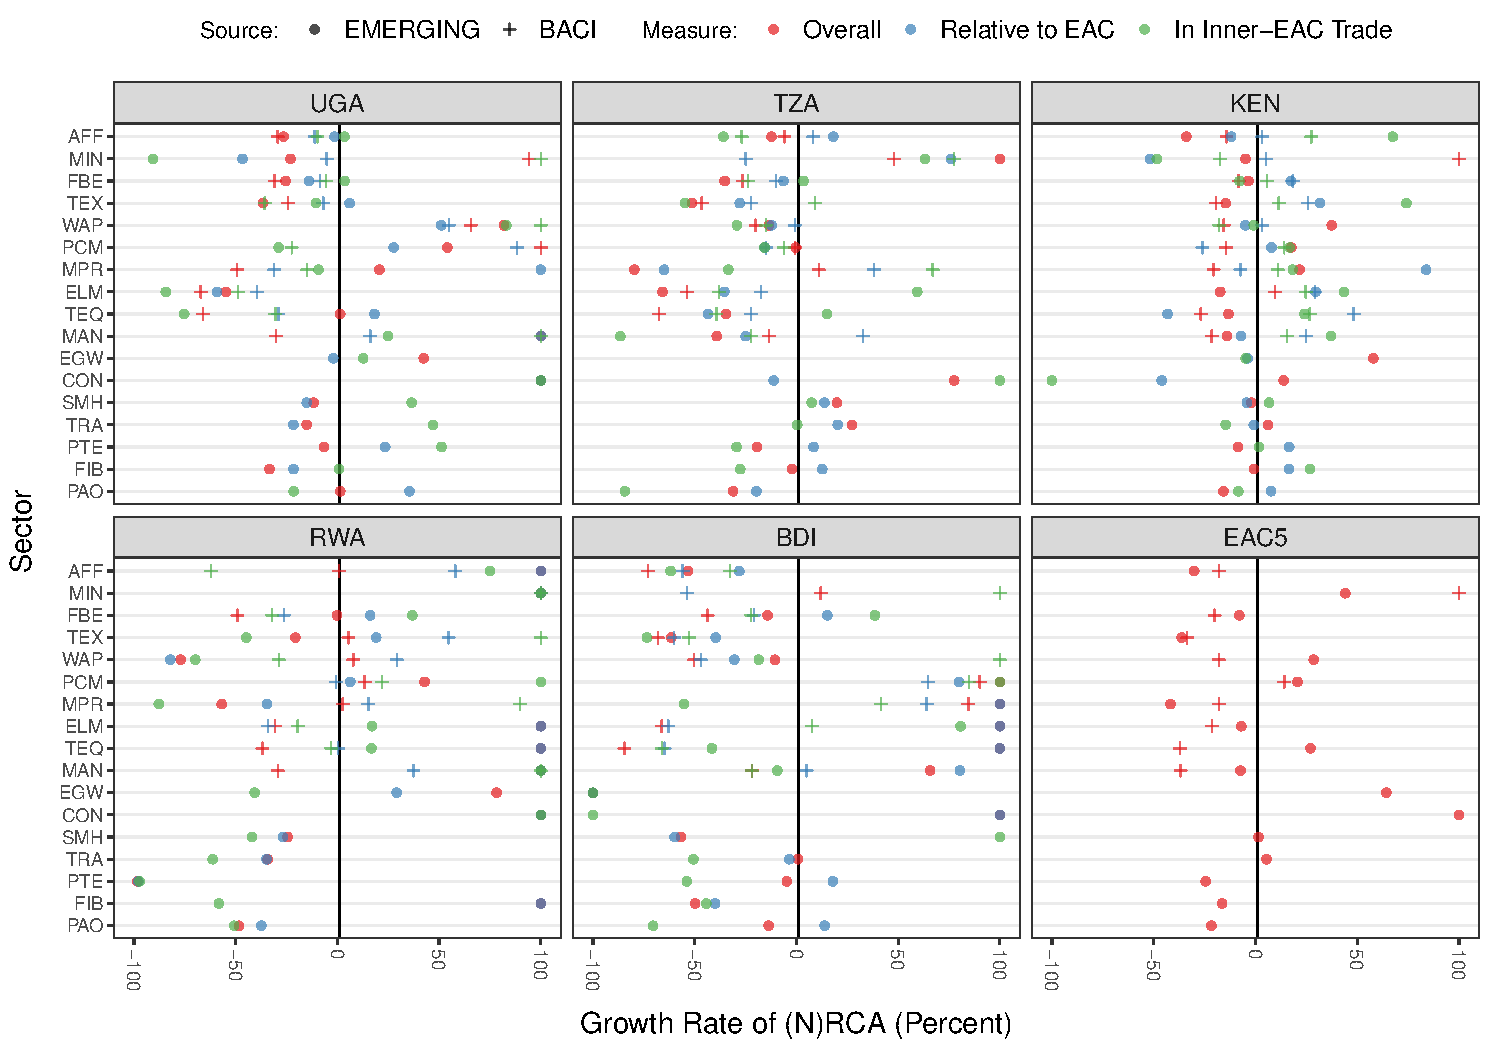
\includegraphics[width=1\textwidth]{"../Figures/REV/NRCA_EAC5_ALL_Growth.pdf"} %trim={<left> <lower> <right> <upper>}
\raggedright
\scriptsize
\emph{Notes:} Figure shows the growth rate in percentage terms between the 2006-10 and 2015-19 (N)RCA medians. EM estimates are based on DVA in exports, BACI on gross exports. Appendix Figure \ref{fig:NRCA_Diff} and Table \ref{tab:NRCA_Diff} show the values. 
\end{figure}
\FloatBarrier

The bottom right panel of Figure \ref{fig:NRCA_GR} shows that the EAC5 as a whole has lost some comparative advantage in AFF, FBE and, in GX terms, in all manufacturing sectors apart from PCM. On the services side there are overall gains in construction (CON), EGW, transport/travel (TRA), and losses in telecommunications (PTE) and financial and business (FIB) services. Relative to the EAC, Kenya gained a bit in FBE, TEX, MPR, and ELM. For core manufacturing sectors this is even more reflected in inner-EAC5 trade, i.e., Kenya's share of EAC manufacturing trade increased, as already noted in section 4.3. These patterns highlight that policy efforts might be needed to strengthen the regions comparative advantage in food processing and tourism, and to reverse the trend towards regional manufacturing trade and value chains that further strengthen Kenya's role as a supplier of intermediates and regional hegemon. 

%In summary, NRCA data support the downstream shift in GVC integration, but the evidence that this is driven by a broad-based decline in manufacturing competitiveness is not as clear as initially presumed. On the other hand, the evidence is compelling insofar that Kenya has a stronger NRCA position in manufacturing than other EAC members, and was the only member able to sustain and slightly enhance its manufacturing position during 2005-2015, while also experiencing a substantially smaller downstream shift (Figure \ref{fig:UP_DOWN_ag_growth}). Other members therewhile became more competitive in agriculture and fishing, and certain services like maintenance and repair activities. \newline
%
%This distribution of comparative advantage encourages less horizontal regional integration, with Kenya increasingly a consumer of raw materials and exporter of manufactured goods vis-a-vis other EAC members. It also implies a rather challenging environment for industrial policy, and the necessity for regional discourse on how EAC economic integration can become more horizontal and foster competitive gains, or at least mitigate competitive losses, for certain members and sectors.  % for members at the top of RVCs. 
%The declared interest of several members, such as Uganda, to strengthen food and beverages manufacturing, could be a fruitful starting point for discussions around RVCs. \newline
%
% The remainder of this paper does little to aid this discussion around the modalities of EAC regional integration but presents some guiding analysis regarding the potential benefits of deeper sector-level integration into GVCs and RVCs for industrial development in the EAC.
 
 % \newpage

\section{GVCs and Industrial Development}

Having extensively documented the patterns of EAC global and regional integration through both traditional trade (Section 3) and value chains (Section 4) while highlighting salient trends, imbalances, and possible policy priorities, an important remaining policy questing regards the impact of different forms of integration on economic development in the region. This section attempts to provide causal reduced-form evidence on this matter, following \citet{Kummritz20161}. \newline

The WDR Chapter 3 presents extensive correlational evidence that GVC participation is associated with gains in GDP per capita growth and labour productivity, poverty reduction, skill transfer and employment creation often benefiting gender equality, but also with challenges in taxation and higher inequality \citep{world2020trading, antras2022global}. The report highlights that the long-term firm-to-firm ans specialization in specific GVC-related tasks promote efficient production, technology diffusion, and access to capital. A cross-country dynamic growth regression estimated with System-GMM yields a 11-14\% improvement in per-capita GDP following a 10\% increase in overall GVC participation, which is contrasted with a 2\% gain from increased trade in products fully produced in one country. The report also shows that countries experience the biggest growth spurt transitioning from commodities to limited manufacturing - 20\% income gains within 3 years. \newline

These findings are broadly echoed in much macroeconomic work on GVCs and economic development. As one of the first, \citet{Kummritz20161} assesses the role of GVCs for labor productivity and domestic VA using OECD ICIOs for 61 countries and 34 industries from 1995-2011. He achieves identification using a novel IV strategy where a VA trade resistance index combining third-country trade costs with industry-specific technological variables induces exogenous variation in GVC participation, and shows that increased GVC participation leads to higher domestic VA and productivity for all countries: a 1 percent increase in backward GVC participation (VS) leads to 0.11\% higher domestic VA in the average industry, and a 1 percent increase in forward GVC participation (VS1) leads to 0.60\% higher domestic VA and 0.33\% higher labor productivity. %The literature as discussed by \citet{Kummritz20161} outlines several channels through which GVC participation (in north-south value chains) increases the VA and productivity of its participants. The main channels are learning-by-doing, technology transfer or spillovers, gains from specialization in comparative advantage tasks, and terms of trade effects. \newline
% Using the same tables, \citep{kummritz20161} also estimates the causal affect of GVC backward and forward participation on industrial development using a novel IV strategy, and finds positive and significant effects on both industrial value-added and labour productivity, especially from forward integration. 
The effects from forward integration are greater for high-income countries, whereas low/middle income countries show stronger returns from backward integration.  % with beneficial effects for domestic industrialization. \newline % \citep{kummritz2015global, }
\citet{altomonte2018trade}, using an instrumental variable combining the growing size of containers ships since 1997 with the ex-ante availability of deep sea ports, also present causal evidence of a positive effect of GVC related trade (DVA in exports) on growth, which is larger than the effect of traditional trade. Both are three-step instrumentation strategies in the spirit of \citet{romer1999does} and \citet{feyrer2009distance, feyrer2019trade}. \newline % provides one such effort at bridging this causality gap: They propose an instru- mental variable based on the availability of port locations that can accommodate mega-container ships; this is shown to predict well a country’s DVA in exports, which in turn is positively linked with growth in income per capita

\citet{constantinescu2019does}, using WIOD with 40 countrie and 13 sectors over 1995-2009, find that GVC participation boost labour productivity, especially use of inputs for export production (backward GVC participation). An increase in GVC participation by 10\% yields an average productivity increase of 1.7\%. Examining a sample of 24 emerging economies \citet{jangam2021does} shows that both forward and backward participation has significantly improved domestic value-added exports over the period 1995–2011. \citet{altun2023does} examine the role of GVC participation in high technology exports for 120 countries during 1995–2019, and find that in GVC participation correlates strongly positively with high-tech exports. \citet{kummritz2017economic} find that GVC participation increases VA, especially in upstream stages. \citet{pahl2020global} study the effects of GVC participation on VA in 58 countries (of which 38 developing) between 1970 and 2008, and find a robust positive effect on manufacturing productivity growth, especially for less productive countries where the distance to the global frontier is large. However, they find no positive effects on employment, and some negative effects for middle-income countries. They thus conclude the GVC participation is a mixed blessing, and induces skill-biased technological change, in-line with \citet{rodrik2018new}. \citet{Kummritz20161} notes that GVCs don't necessarily need to benefit developing countries as there could be adverse terms of trade effects or decreases in productive endowments from heavy engagement in them, which is also shown in some theoretical models such as \citet{baldwin2014trade}. An argument made by \citet{kummritz2015global} is also that GVCs might substitute foreign for domestic suppliers, but his own empirical research suggests that foreign VA works as a complement rather than a substitute to domestic VA. \newline % and that GVC participation benefits the domestic economy along the value chain if certain prerequisites are met. 
 % \citet{kummritz2015global} finds no significant effect of GVC participation on low-income countries, which he attributes to the low absorptive capacity to benefit from technology spillovers. The micro-papers discussed however point towards an overwhelmingly positive effect. \newline
 
 Further empirical evidence on the relationship between domestic value chains and GVCs is provided by \citet{beverelli2019domestic}. They find that across countries at different stages of development, higher domestic integration by 1 standard deviation raises subsequent GVC integration through backward linkages (VS) by 0.4\%. They also find that domestic value chain integration explains up to 30\% of overall GVC integration. They explain these results with fixed costs of fragmentation and switching suppliers: "high fragmentation costs allow, due to their sunk nature, DVCs to act as stepping stones to GVCs" \citep{beverelli2019domestic}. \newline %The results imply that improving domestic economic integration would further GVC integration in the medium run. % \newline

\citet{shen2021towards} construct a simple dynamic model to illustrate the micro-mechanism of industrial upgrading along the global value chains. Using the WIOD, they find that more upstream industries are correlated with higher profitability and value-added as well as higher capital intensity and R\&D investment. Their dynamic model explains this through three effects: endogenous sunk costs, descreasing intermediate input price elasticity, and sequential pricing effect uncertainty. They show that the empirical patterns revealed in China are consistent with the model's predictions. \citet{tian2022global} also study the relationship between GVC participation and industrial upgrading (process, product and skill upgrading) using the WIOD. They find that GVC integration increases industrial upgrading for both developing and developed countries. Developing countries benefit more from backwards GVC participation through importing more sophisticated inputs and learning through embodied knowledge, whereas developed countries upgrade more through forward GVC participation. Overall, they interpret their findings as evidence against more critical voices and models quaestioning the benefits of developing country participation in GVCs, such as \citet{baldwin2014trade} or \citet{dalle2013industrial}. \newline
% Our empirical results did not provide very solid evidence for developing countries that forward GVC participation benefits their upgrading. -> your findings do suggest that !

The macroeconomic study of \citet{lwesya2022integration} on GVCs and economic upgrading in the EAC, discussed in the introduction, also finds a significant positive effect of lagged foreign VA on domestic VA in EAC5 exports, with coefficients implying an elasticity of 0.49. \newline 

Many microeconomic studies also find positive effects of GVC participation for industrial development. \citet{piermartini2014knowledge} for example use industry-level R\&D and patent data for a sample of 29 countries during the period 2000-2008 and show that knowledge spillovers increase with the intensity of supply chains linkages between countries and that these spillovers are larger in magnitude than spillovers from traditional trade flows. Similar evidence is presented by \citet{benz2015trade}, who use firm-level data to show that offshoring leads to knowledge spillovers and forward spillovers (from producers to users if intermediate inputs) are stronger than backward spillovers. \citet{durongkaveroj2023emphasis} studies GVC participation and export earnings at the industry-level in Thailand, and finds that there is no significant relationship between domestic value added and net-export earnings, but greater participation in GVCs significantly increases export performance. \newline

Microeconomic studies involving EAC members include \citet{barrientos2016shifting}'s case study of supermarket expansion within South and East Africa, showing that higher quality and sourcing requirements by global and regions supermarket chains induced improved processes in Kenyan and Ugandan horticulture, allowing diversification and higher fruits and vegetable exports \citep{world2020trading}. A study of Kenyan horticulture by \citet{krishnan2018origin} shows that incomes increased after contract farmers adopted quality standards by their international buyers, and also that opportunistic RVCs emerged when suppliers found their produce rejected due to lack of standards compliance, which gradually led to more organized RVCs with own standards and procurement strategies. \citet{dihel2018does} study the effects of value chains participation on African Farmers via a survey of 3,935 farmers, 60 aggregators, and 56 buyers in the maize, cassava, and sorghum value chains in Ghana, Kenya and Zambia, and show that contracted farmers saw greater structural transformation; higher output; and better access to seeds, fertilizers, pesticides, technology, and extension services than non-contracted farmers. These findings are commensurate with \citet{daly2016maize}'s study of Maize value chains in east Africa, which identifies Kenyan processors as the lead firms demanding Ugandan suppliers to provide high-quality maize, and document investments into Ugandan production facilities by South African and German companies, but also document challenges in access to finance for farmers, commercial scale, and lack of communication of market signals and standards along the value chain.    \newline

While these microeconomic studies point towards positive growth effects and upgrading prospects from EAC  engagement in agricultural and food processing GVCs, a study on mining value chains in Latin America by \citet{pietrobelli2018innovation} suggests that a hierarchical value chain, dominated by few large firms, and poor linkages (e.g. large mining firms rarely forge long-term links with local suppliers or collaborate with them on innovative projects) is blocking the diffusion of innovations and hindering suppliers’ development \citep{pietrobelli2018innovation, world2020trading}. 


% Several papers assess the links between GVC integration and industrial development. 
% More recent empirical work has focused more strongly on specific aspects of GVC integration, such as domestic content in exports, GVC positioning, and the relationship of GVC and traditional trade.  

 
 

\newpage









% \subsection{GVC Integration and Domestic VA}
\subsection{Empirical Strategy}


A natural idea to assess the impact of GVC integration on industrial development is to investigate if higher imported or re-exported content in exports is associated with higher domestic VA produced i.e. higher GDP. This is done in one form or another by many authors, including \citet{lwesya2022integration} who use DVA in exports. I argue however, in line with \citep{rodriguez2000trade} and \citet{Kummritz20161}, that running regressions at the country-level is subject to omitted variable bias from many factors affecting both GVC integration and economic development. Thus a sector-level regression framework with country-sector, country-year and sector-year fixed effects is highly advantageous to capture many confounding factors identified in both the development (such as infrastructure, geography, institutions and economic policies) and trade (such as multilateral resistance) literatures. A caveat is that the measured effects are within-industry effects, and therefore likely a lower bound on the overall economic effects of GVC integration. The baseline specification is 
\begin{equation} \label{eq:VA_HDFE}
\log(\text{VA}_{cst}) = \beta \log(\text{GVC}_{cst}) + \alpha_{cs} + \beta_{ct} +\gamma_{st} + \epsilon_{cst},
\end{equation}
where $\textbf{GVC}_{cst}$ is a GVC indicator (such as forward of backward GVC participation), and 
$\alpha_{cs}$, $\beta_{ct}$, and $\gamma_{st}$ are country-sector, country-year and sector-year fixed effects, respectively. This specification is also biased due to potential sector-level omitted variables, measurement error in GVC participation, simultaneity and reverse causality.  \newline

To address these issues, I follow \citet{Kummritz20161} in developing an instrument for GVC participation at the bilateral-sector-level that uses third-party trade costs multiplied by the distance of industries in the value chain to induce exogenous variation in foreign VA in exports which forms the basis for simple VS and VS1 (E2R) GVC indicators. I refer the reader to \citet{Kummritz20161} for a more extensive treatment of this instrumentation strategy, but the basic idea is to predict the elements of the \textbf{VBE} matrix using exogenous trade costs and industry structure, and then compute VS and VS1 indicators following Equations \ref{eq:VS} and \ref{eq:VS1} using this predicted matrix $\hat{\textbf{VBE}}$, to obtain exogenous components $\hat{\text{VS}}_{uj}$ and $\hat{\text{VS1}}_{oi}$, which can be then used to instrument the VS and VS1 measures in a sector-level FE regression. Specifically, for each GVC instrument a different $\hat{\textbf{VBE}}_t$ matrix is constructed, whose (time-varying) elements $vbe_{oiujt}$ are predicted using equations
\begin{align} \label{eq:predVS}
\hat{vbe}_{oiujt}^\text{VS} &= \exp(\beta^\text{VS} \log(\tau_{out}\times \delta_{oiuj}) + \alpha_{uj} + \beta_{ut} +\gamma_{jt} + \epsilon_{oiujt}) \quad \forall\  u\neq o \\ \label{eq:predVS1}
\hat{vbe}_{oiujt}^\text{VS1} &= \exp(\beta^\text{VS1} \log(\tau_{out}\times \delta_{oiuj}) + \alpha_{oi} + \beta_{ot} +\gamma_{it} + \epsilon_{oiujt}) \quad \forall\  o\neq u
\end{align}
to construct $\hat{\text{VS}}_{uj}$ and $\hat{\text{VS1}}_{oi}$, respectively. $\hat{\text{VS}}_{ujt}$ is then obtained by summing column $uj$ of a matrix $\hat{\textbf{VBE}}_t^\text{VS}$ where domestic elements are set to zero and the non-domestic ($u\neq o$) elements are estimated using Eq. \ref{eq:predVS}, which includes fixed effects for the using country-sector ($uj$) and time ($ut$, $jt$) dimensions (as in the final stage model). Thus all variation in the (time-varying) foreign sources of VA ($oit$) and in the time-varying usage ($ujt$), is predicted by the exogenous trade cost term: $\log(\tau_{out}\times \delta_{oiuj})$. Similarly, Eq. \ref{eq:predVS1} estimates $\hat{\textbf{VBE}}_t^\text{VS1}$ to obtain $\hat{\text{VS1}}_{oit}$. \newline

The trade cost term is composed of two components: $\tau_{out}$ is an export weighted estimate of the bilateral trade costs of the supplier of VA $o$ with all other trading partners $k\neq u$ in period $t$. This, following \citet{Kummritz20161}, is done to preserve exogenity of the trade cost measure to factors affecting the specific of the bilateral $ou$ link, which may be correlated with GVC related trade along this link. I follow \citet{Kummritz20161} in using the World Bank ESCAP trade costs database \citep{arvis2016trad} based on \citet{novy2013gravity}, which provides a holistic, tariff-equivalent measure of total trade costs implied by an inverse gravity model. \newline %\todo{Plot Trade cost measure within the EAC + Table}. \newline 

The second term, $\delta_{oiuj}$, is a time-invariant measure of the distance between industries $oi$ and $uj$ along the GVC. It is defined as $\delta_{ijt} = 1/(u_{oi}\times d_{uj})$, where $u_{oi} = \frac{1}{T}\sum_t u_{oit}$ is the average upstreamness of country-sector $oi$ as defined in Eq. \ref{eq:upstreamness} and $d_{jt} = \frac{1}{T}\sum_t d_{ujt}$ a corresponding downstremness index, as described e.g. in \citet{antras2022global} and footnote 15. \citet{Kummritz20161} notes that the indirect trade costs ($\tau_{out}$) have a larger effect on VA for industries separated by more stages ($\delta_{oiuj}$). The index $\delta_{oiuj}$ is inverted since $u_{oi}$ and $d_{uj}$ have a positive relationship with the elements of \textbf{VBE}, to yield a trade cost index $\tau_{out}\times \delta_{oiuj}$ negatively related to $vbe_{oiujt}$. \newline 
% Previous Solution: 
%I finally note that in the MRIO, upstreamness and downstreamness are computed separately for each country-industry, but I use $u_{it} = \frac{1}{n}\sum_o u_{oit}$ and $d_{jt} = \frac{1}{n}\sum_u d_{uit}$, i.e. I take the arithmetic average across countries to obtain indices for each industry and time period in order to allow for changing technology affecting the general relative position of sectors, while avoiding confounding influences from specific bilateral relative industry positions, which may be correlated with the VA trade flows along this link. Unlike \citet{Kummritz20161} who also aggregates over time, I preserve the time dimension (which accounts for about 3\% of the variance of the industry-aggregates) because of the extended EORA time dimension (\citet{Kummritz20161} uses OECD tables for 5 periods). Also in addition to \citet{Kummritz20161}, I smooth both the trade cost measure ($\tau_{out}$) and the upstreamness and downstreamness measures using a centered 3-year moving average, based on the observation that trade costs based on an inverted gravity model are somewhat endogeneous to current trade flows, and therefore more volatile than pure technological or regulatory changes would warrant.   \newline 

In addition to \citet{Kummritz20161}, I also employ an industry distance measure $\delta_{oiuj}$ at the country-sector level, whereas he uses a measure $\delta_{ij}$ of pure industry distance that is averaged across countries as well. While this common technology assumption may be appropriate for his sample of mostly OECD economies in the OECD TIVA ICIO tables, I find that the instrument constructed using this formulation lacks relevance for my core EAC5 sample. This indicates that industries in developing countries may use different technologies and have different GVC positions than the same industries in advanced economies. While using a bilateral-sector-level industry distance measure may partly compromise the exogeneity of the instrument, I argue that this is unlikely because this distance is still time invariant, and the 2SLS regressions include a full set of country-sector, country-year and sector-year fixed effects. Thus the identifying variation still comes from the trade cost term ($\tau_{out}$), and using a more accurate measure of industry distance merely helps increase the relevance of this term. Empirically, I find that computing two instruments using both $\delta_{oiuj}$ and $\delta_{ou}$ and including them both in the first stage yields a sizeable improvement in the fit, indicating that the difference of local industry structure to the world average interacted with trade costs is a reasonable predictor of foreign VA in developing countries. In all cases the instruments are very weak, and results must be interpreted with caution.  \newline

Another difference to \citet{Kummritz20161} is that I smooth bilateral trade costs using a centered 3-year moving average and impute missing values at the end of the sample using the last MA observation carried forward. This is sensible because trade costs based on an inverted gravity model are endogeneous to current trade flows, and therefore more volatile than pure technological or regulatory changes would warrant. The smoothing step also does not compromise the relevance of the instrument, confirming that the raw trade cost measure is noisy. Appendix Figure \ref{fig:ESCAP_EAC} shows the raw and smoothed bilateral trade costs among EAC5 members. Interestingly, the   ESCAP estimates suggest that trading with Kenya is significantly less costly for members than trading with other members, i.e., only with Kenya total trade costs are estimated below an 100\% ad-valorem Tariff equivalent, and Kenya and Uganda also report trade costs well below 100\% on each other. These costs are, of course, fully endogenous to observed trade flows, and the strong trade links between Kenya and Uganda were already highlighted several times in this paper. This perspective however entertains a thus far neglected possibility that asymmetric trading costs may be another reason for sluggish and asymmetric EAC integration in supply chain trade. In the framework of \citet{antras2020geography}, high trade costs imply a greater importance for regional GVC participation. %\todo{Make this point further below as it may affect returns to RI.}
Since the IV trade cost measure ($\tau_{out}$) is a weighted average of origin's ($o$) trade costs with third parties, and EAC members trade much more with ROW than with each other, an accurate and timely representation of regional trade costs is irrelevant for the IV. \newline
% \todo[inline]{Country-sector-level upstreamness and downstreamness is endogeneous to country GVC integration, so need to use $\delta_{ijt}$ instead of $\delta_{oiujt}$!!}

In addition to estimating returns to backward and forward GVC integration, I also consider returns to gross trade, trade in final goods, and measures of regional integration introduced in Section 4.3, in  particular VS$^\text{EAC}$ and VS1$^\text{EAC}$. Since these are components of VS and VS1, the construction of appropriate instruments is straightforward. For gross and final goods trade, I omit the industry distance component and instead construct a sector-level time-varying 3rd-party trade cost measure $\tau_{oiut}$ which is obtained as the exports-weighted average of sector $i$ in country $o$'s exports to all destination counties $k \neq u$. \newline 

My default sample includes the full number of sectors (26 for EORA, 134 for EMERGING), for 5 EAC countries: Uganda, Rwanda, Tanzania, Kenya and Burundi. South Sudan is omitted because of data quality concerns, Congo because of lacking RVC integration with the EAC and different (more resource intense) trading patterns. The inclusion of Congo does not significantly alter the results\todo{Report in Appendix.}. Estimations are run using indicators computed on EORA 2021, the GVC indicators from the 2020 WDR using EORA 2015, and indicators computed using EMERGING. With each database, I run one set of estimations using the full set of sectors, and one using only manufacturing sectors (all sectors mapping to broad sectors FBE, TEX, WAP, PCM, MPR, ELM, TEQ, MAN, in Table \ref{tab:sec}). Unfortunately, in all estimations with EMERGING, the coefficients, both OLS and IV, are statistically insignificant and close to zero. This indicates that the full sectoral resolution of 134 sectors in these tables is not suitable to evaluate returns to trade and GVC particpation in the EAC5. Unfortunately, aggregating to broad sectors also yields insignificant results due to the short time dimension of only 6 years of data. Thus I do not report EMERGING results in the main paper. The following sections report the results based on EORA, starting with gross trade.


\subsection{Results: Gross Trade and Trade in Final Goods}

Table \ref{tab:FS_GT_RES} shows results for gross trade using the full sample of sectors, and Table \ref{tab:MS_GT_RES} shows identical regressions for the subset of manufacturing sectors. In both tables the instruments are weak, and with one exception, not significantly different from OLS. The OLS results suggest an elasticity of VA tp gross trade of 0.13-0.25, in-line with the 0.2 reported by the WDR. The results are also congruent to \citet{altomonte2018trade}, who find larger effects around 0.3 using the WIOD, but also very similar OLS and IV coefficients, with IV being slightly larger than OLS. The effects of trade in final goods on VA are slightly lower at 0.1-0.2, and effects of both gross and final goods trade in manufacturing sectors (Table \ref{tab:MS_GT_RES}) are even lower at $\leq 0.1$. This indicates that intermediates trade, i.e., GVC related trade, is more important for economic development in the EAC, particularly for manufacturing sectors where intermediates account for a larger fraction of total trade. 


\begin{table}[h!]
   \caption{\label{tab:FS_GT_RES} Gross Trade: EAC5 IV Regression using EORA26}
   \centering
  \resizebox{\textwidth}{!}{
   \centering
   \begin{tabular}{lcccccccc}
      \tabularnewline \midrule \midrule
      Dependent Variable: & \multicolumn{8}{c}{log(VA)}\\
      Data: & \multicolumn{2}{c}{EORA21} & \multicolumn{2}{c}{EORA15} & \multicolumn{2}{c}{EORA21} & \multicolumn{2}{c}{EORA15} \\
                                          & OLS    & IV            & OLS    & IV            & OLS    & IV    & OLS    & IV \\    
      Model:                              & (1)            & (2)                   & (3)            & (4)                   & (5)            & (6)           & (7)            & (8)\\  
      \midrule
      \emph{Variables}\\
      log(E)                              & 0.2454$^{***}$ & 0.1072                & 0.1305$^{***}$ & 0.1503$^{*}$          &                &               &                &   \\   
                                          & (0.0419)       & (0.0770)              & (0.0233)       & (0.0777)              &                &               &                &   \\   
      log(Efd)                            &                &                       &                &                       & 0.1892$^{***}$ & 0.1931$^{**}$ & 0.1036$^{***}$ & 0.1776$^{**}$\\   
                                          &                &                       &                &                       & (0.0353)       & (0.0818)      & (0.0207)       & (0.0719)\\   
      \midrule
      \emph{Fixed-effects}\\
      \# country-sector                   & 130            & 130                   & 129            & 129                   & 130            & 130           & 129            & 129\\  
      \# country-year                     & 110            & 110                   & 80             & 80                    & 110            & 110           & 80             & 80\\  
      \# sector-year                      & 572            & 572                   & 416            & 416                   & 572            & 572           & 416            & 416\\  
            \midrule
      \emph{Fit statistics}\\
      Observations                        & 2,740          & 2,740                 & 2,023          & 2,023                 & 2,740          & 2,740         & 2,023          & 2,023\\  
      R$^2$                               & 0.9859         & 0.9856                & 0.9928         & 0.9928                & 0.9855         & 0.9855        & 0.9927         & 0.9927\\  
      Within R$^2$                        & 0.0485         & 0.0331                & 0.0238         & 0.0232                & 0.0269         & 0.0269        & 0.0143         & 0.0070\\  
      Wu-Hausman, p-value                 &                & 0.0101                &                & 0.5572                &                & 0.9703        &                & 0.0819\\  
      Kleibergen-Paap (1st stage), F &           & 23.99                 &                & 28.82                 &                & 3.086         &                & 20.28\\  
      Wald (1st stage), p-value   &                & $<0.001$              &                & $<0.001$              &                & 0.0790               &   & $<0.001$             \\  
      \midrule \midrule
      \multicolumn{9}{l}{\emph{Driscoll-Kraay (L=2) standard-errors in parentheses}}\\
      \multicolumn{9}{l}{\emph{Signif. Codes: ***: 0.01, **: 0.05, *: 0.1}}\\
   \end{tabular}
   }
\end{table}
\FloatBarrier



\begin{table}[h!]
   \caption{\label{tab:MS_GT_RES} Gross Trade: EAC5 IV Regression using EORA26: Manufacturing Sectors}
   \centering
  \resizebox{\textwidth}{!}{
   \centering
   \begin{tabular}{lcccccccc}
      \tabularnewline \midrule \midrule
      Dependent Variable: & \multicolumn{8}{c}{log(VA)}\\
      Data: & \multicolumn{2}{c}{EORA21} & \multicolumn{2}{c}{EORA15} & \multicolumn{2}{c}{EORA21} & \multicolumn{2}{c}{EORA15} \\
                                          & OLS    & IV            & OLS    & IV            & OLS    & IV    & OLS    & IV \\    
      Model:                              & (1)            & (2)                   & (3)            & (4)                   & (5)            & (6)           & (7)            & (8)\\  
      \midrule
      \emph{Variables}\\
      log(E)                              & 0.1015$^{***}$ & 0.9659      & 0.1175$^{***}$ & 0.2198      &              &             &                &   \\   
                                          & (0.0324)       & (0.6435)    & (0.0299)       & (0.1746)    &              &             &                &   \\   
      log(Efd)                            &                &             &                &             & -0.0566      & -0.1048     & 0.1075$^{***}$ & -0.0211\\   
                                          &                &             &                &             & (0.0920)     & (0.5590)    & (0.0303)       & (0.0400)\\   
      \midrule
      \emph{Fixed-effects}\\
      \# country-sector                   & 40           & 40                   & 40            & 40                   & 40            & 40           & 40            & 40\\  
     \# country-year                     & 110            & 110         & 80             & 80          & 110          & 110         & 80             & 80\\  
      \# sector-year                      & 176            & 176         & 128            & 128         & 176          & 176         & 128            & 128\\ 
            \midrule
      \emph{Fit statistics}\\
     Observations                        & 859            & 859         & 640            & 640         & 859          & 859         & 640            & 640\\  
      R$^2$                               & 0.9883         & 0.9817      & 0.9951         & 0.9951      & 0.9882       & 0.9882      & 0.9951         & 0.9950\\  
      Within R$^2$                        & 0.0077         & -0.5515     & 0.0216         & 0.0052      & 0.0022       & 0.0006      & 0.0216         & -0.0093\\  
      Wu-Hausman, p-value                 &                & 0.1060      &                & 0.7317      &              & 0.9675      &                & 0.5074\\  
      Kleibergen-Paap (1st stage), F &           & 1.009       &                & 5.278       &              & 0.4104      &                & 19.31\\ 
      Wald (1st stage), p-value   &                & 0.3152      &                & 0.0218             &                & 0.5217      &                & $<0.001$ \\  
      \midrule \midrule
      \multicolumn{9}{l}{\emph{Driscoll-Kraay (L=2) standard-errors in parentheses}}\\
      \multicolumn{9}{l}{\emph{Signif. Codes: ***: 0.01, **: 0.05, *: 0.1}}\\
   \end{tabular}
   }
\end{table}
\FloatBarrier


\subsection{Results: Backward and Forward GVC Participation}

Appendix Tables \ref{tab:ZS_FULL} and \ref{tab:ZS_EAC} shows the zero stage regressions predicting the elements $vbe_{oiujt}$ using the full sample and EAC5 sample, respectively. Evidently, the trade cost measures are negatively correlated with the elements of \textbf{VBE}. %\newline %  in both databases. 
I then run both OLS and 2SLS fixed-effects regressions according to Eq. \ref{eq:VA_HDFE} using VS and VS1 measures in log-levels and instrumenting them with $\hat{\text{VS}}$ and $\hat{\text{VS1}}$, also in log-levels. %I use corrected VS1 following \citet{borin2019measuring} in the second stage, whereas the instrument $\hat{\text{VS1}}$ is based on the naive version (E2R) following Eq. \ref{eq:VS1}. This is unlikely to be a great issue, as both measures are highly correlated, and an unbiased estimate of the first-stage regression coefficient is not of interest. 
I estimate 4 specifications: (1) OLS, (2) IV with the time-invariant ($\delta_{ij}$) industry-distance instrument,  (2) IV with the bilateral ($\delta_{oiuj}$) industry-distance instrument, and (4) IV with both instruments. \newline

Table \ref{tab:FS_RES} shows the results on the full sample, and Table \ref{tab:MS_RES} the results for the manufacturing sample. Appendix Tables \ref{tab:FS_RES_F1} and \ref{tab:MS_RES_F1} report the corresponding first stages. An analysis with aggregated sectors as in Table \ref{tab:sec} therefore follows, which is more fruitful. A second thing to note from Tables \ref{tab:FS_RES_F1} and \ref{tab:MS_RES_F1}, is that the 2SLS first stages are generally very weak, with many coefficients insignificant or of the wrong sign. Since the trade cost measure $\tau_{out}\times \delta_{oiuj}$ is negatively correlated with value added, these negative first-stage coefficients could indicate some overfitting at the zero stages (Tables \ref{tab:ZS_FULL} and \ref{tab:ZS_EAC}) which are also quite weak. In any case, this indicates that the 2SLS results in Tables \ref{tab:FS_RES} and \ref{tab:MS_RES} need to be treated with extreme caution and skepticism, even in cases where first-stage statistics at the bottom of these tables (such as a sizeable F-statistic) suggest that the first stages are valid. In all estimations, the instruments are very weak. Another notable fact is that coefficients from the full EORA 200-2021 sample are generally smaller and more often insignificant than those of WDR (EORA 2000-2015) sample. This appears to reflect the structural break (which is absorbed by the fixed effects) and (more importantly) subsequent change in trend induced in 2016. Thus I consider the results on the WDR sample more reliable, as the data here at least reflect a consistent methodology and temporal variation over the entire sample. \newline


\todo[inline]{Report Kleinbergen \& Paap robust F-statistic, eliminate conventional one}

\todo[inline]{Consider simple lag specification where both indicators are lagged one period (including IV, no contemporaneous term). Or: Dynamic IV, with simple contemporaneous first stage.  Or dynamic first stage?}

\begin{table}[h!]
   \caption{\label{tab:FS_RES} Full Sample IV Regression using EORA26}
   \centering
  \resizebox{\textwidth}{!}{
   \begin{tabular}{lcccccccc}
      \tabularnewline \midrule \midrule
      Dependent Variable: & \multicolumn{8}{c}{log(VA)}\\
      Data: & \multicolumn{4}{c}{EORA21 (2000-2021)} & \multicolumn{4}{c}{WDR EORA15 (2000-2015)} \\
      Model:                  & OLS            & IV-$\delta_{ij}$      & IV-$\delta_{oiuj}$    & IV-Both               & OLS      & IV-$\delta_{ij}$      & IV-$\delta_{oiuj}$    & IV-Both\\  
      \midrule
      \emph{Variables}\\
      log(VS)                 & -0.2007$^{**}$ & 0.5918                & 0.6157                & 0.2340$^{**}$         & -0.0389  & 0.2045$^{***}$        & 0.2091$^{***}$        & 0.1915$^{***}$\\   
                              & (0.0822)       & (0.4165)              & (0.4500)              & (0.0832)              & (0.0447) & (0.0415)              & (0.0410)              & (0.0433)\\  
      \emph{Fit statistics}\\
      Observations            & 2,740          & 2,740                 & 2,740                 & 2,740                 & 2,023    & 2,023                 & 2,023                 & 2,023\\  
      R$^2$                   & 0.9857         & 0.9777                & 0.9772                & 0.9833                & 0.9927   & 0.9920                & 0.9920                & 0.9921\\  
      Within R$^2$            & 0.0345         & -0.5034               & -0.5363               & -0.1273               & 0.0023   & -0.0861               & -0.0894               & -0.0769\\  
      Wu-Hausman, p-value     &                & $<0.001$  & $<0.001$  & $<0.001$  &          & $<0.001$  & $<0.001$  & $<0.001$\\   
      F-statistic (1st stage)        &                    & 81.57                 & 77.42                  & 66.67                  &                    & 464.7                 & 458.8                  & 235.8\\  
      Wald (1st stage), p-value &                    & 0.2163                & 0.2318                 & $<0.001$  &                    & $<0.001$  & $<0.001$  & $<0.001$\\  
      \midrule
       \emph{Variables}\\
      log(E2R)                & 0.7351$^{***}$     & 0.1842                & -0.1586                & -0.6351               & 0.7432$^{***}$     & 0.5716$^{***}$        & 0.5359$^{**}$          & 0.7366$^{***}$\\   
                              & (0.0396)           & (1.129)               & (2.588)                & (2.591)               & (0.0607)           & (0.1831)              & (0.1907)               & (0.0597)\\ 
      \emph{Fit statistics}\\
      Observations            & 2,740              & 2,734                 & 2,733                  & 2,733                 & 2,023              & 2,017                 & 2,016                  & 2,016\\  
      R$^2$                   & 0.9950             & 0.9894                & 0.9803                 & 0.9608                & 0.9976             & 0.9973                & 0.9972                 & 0.9976\\  
      Within R$^2$            & 0.6633             & 0.2889                & -0.3138                & -1.618                & 0.6683             & 0.6329                & 0.6164                 & 0.6724\\  
      Wu-Hausman, p-value     &                    & 0.0678                & 0.0568                 & 0.0016                &                    & 0.0638                & 0.0460                 & 0.8330\\  
      F-statistic (1st stage)       &                    & 3.951                 & 1.654                  & 0.9695                &                    & 38.84                 & 31.31                  & 26.93\\  
      Wald (1st stage), p-value &                    & 0.5067                & 0.6920                 & 0.7512                &                    & 0.0645                & 0.0459                 & 0.0137\\ 
      \midrule
      \emph{Fixed-effects}\\
      \# country-sector       & 130            & 130                   & 130                   & 130                   & 129      & 129                   & 129                   & 129\\  
      \# country-year         & 110            & 110                   & 110                   & 110                   & 80       & 80                    & 80                    & 80\\  
      \# sector-year          & 572            & 572                   & 572                   & 572                   & 416      & 416                   & 416                   & 416\\  
      \midrule \midrule
      \multicolumn{9}{l}{\emph{Driscoll-Kraay (L=2) standard-errors in parentheses}}\\
      \multicolumn{9}{l}{\emph{Signif. Codes: ***: 0.01, **: 0.05, *: 0.1}}\\
   \end{tabular}
   }
\end{table}
\FloatBarrier


\begin{table}[h!]
   \caption{\label{tab:MS_RES} Manufacturing Sample IV Regression using EORA26}
   \centering
  \resizebox{\textwidth}{!}{
   \begin{tabular}{lcccccccc}
      \tabularnewline \midrule \midrule
      Dependent Variable: & \multicolumn{8}{c}{log(VA)}\\
      Data: & \multicolumn{4}{c}{EORA21 (2000-2021)} & \multicolumn{4}{c}{WDR EORA15 (2000-2015)} \\
      Model:                  & OLS            & IV-$\delta_{ij}$      & IV-$\delta_{oiuj}$    & IV-Both               & OLS      & IV-$\delta_{ij}$      & IV-$\delta_{oiuj}$    & IV-Both\\  
      \midrule
      \emph{Variables}\\
      log(VS)                 & 0.1336$^{***}$     & 1.415                 & 1.654                  & 0.4800$^{**}$         & 0.0584$^{*}$       & 0.4380$^{***}$        & 0.4546$^{***}$         & 0.2097$^{***}$\\   
                              & (0.0227)           & (1.981)               & (2.832)                & (0.1834)              & (0.0292)           & (0.1166)              & (0.1233)               & (0.0462)\\   
      \emph{Fit statistics}\\
      Observations            & 859                & 859                   & 859                    & 859                   & 640                & 640                   & 640                    & 640\\  
      R$^2$                   & 0.9884             & 0.9684                & 0.9602                 & 0.9870                & 0.9951             & 0.9940                & 0.9939                 & 0.9949\\  
      Within R$^2$            & 0.0185             & -1.684                & -2.377                 & -0.1058               & 0.0053             & -0.2173               & -0.2372                & -0.0301\\  
      Wu-Hausman, p-value     &                    & 0.0970                & 0.1156                 & 0.0010                &                    & 0.0025                & 0.0027                 & 0.0239\\  
      F-statistic (1st stage)       &                    & 2.433                 & 1.555                  & 64.88                  &                    & 61.72                 & 55.70                  & 109.0\\  
      Wald (1st stage), p-value &                   & 0.4947                & 0.5814                 & $<0.001$  &                    & $<0.001$  & $<0.001$   & $<0.001$\\
      \midrule
       \emph{Variables}\\
      log(E2R)                & 0.6724$^{***}$     & 0.8149$^{***}$         & 0.8204$^{***}$         & 0.8366$^{***}$         & 0.5275$^{***}$     & 1.094$^{***}$         & 1.214$^{***}$          & 0.7602$^{**}$\\   
                              & (0.0775)           & (0.0377)               & (0.0390)               & (0.0443)               & (0.1523)           & (0.3019)              & (0.3362)               & (0.2842)\\ 
      \emph{Fit statistics}\\
      Observations            & 859                & 859                    & 859                    & 859                    & 640                & 640                   & 640                    & 640\\  
      R$^2$                   & 0.9966             & 0.9963                 & 0.9962                 & 0.9961                 & 0.9978             & 0.9946                & 0.9932                 & 0.9972\\  
      Within R$^2$            & 0.7148             & 0.6827                 & 0.6801                 & 0.6721                 & 0.5496             & -0.0841               & -0.3807                & 0.4427\\  
      Wu-Hausman, p-value     &                    & 0.0002                 & $<0.001$               & $<0.001$               &                    & 0.1988                & 0.1378                 & 0.5741\\  
      F-statistic (1st stage)        &                    & 182.2                 & 200.0                  & 113.9                  &                    & 1.792                 & 1.627                  & 1.016\\  
      Wald (1st stage), p-value &                    & 0.0062                & 0.0022                 & $<0.001$  &                    & 0.0006                & 0.0027                 & 0.0009\\ 
      \midrule
      \emph{Fixed-effects}\\
      \# country-sector       & 40                 & 40                    & 40                     & 40                    & 40                 & 40                    & 40                     & 40\\  
      \# country-year         & 110                & 110                   & 110                    & 110                   & 80                 & 80                    & 80                     & 80\\  
      \# sector-year          & 176                & 176                   & 176                    & 176                   & 128                & 128                   & 128                    & 128\\ 
      \midrule \midrule
      \multicolumn{9}{l}{\emph{Driscoll-Kraay (L=2) standard-errors in parentheses}}\\
      \multicolumn{9}{l}{\emph{Signif. Codes: ***: 0.01, **: 0.05, *: 0.1}}\\
   \end{tabular}
   }
\end{table}
\FloatBarrier

\newpage

The results overall suggest that GVC participation has a positive effect on domestic VA, and that this effect is larger for forward integration (E2R) and for manufacturing sectors. Drawing from the IV results in the WDR sample, a 1\% increase in the foreign content of exports (VS) implies a 0.2\% increase in domestic VA (GDP at basic prices minus taxes or subsidies) in the full sample of sectors, and a 0.45-0.5\% increase in manufacturing VA. A 1\% increase in the re-exported content of exports (E2R) on the other hand implies a 0.5-0.7\% increase in domestic VA, and a 0.8-1\% increase in manufacturing VA. \newline

Larger productivity gains from forward integration (E2R) are also prevalent in the literature. \citet{Kummritz20161}, using the 54 countries (among which 28 are low or middle income, but none in Africa) and 20 industries (of which 14 manufacturing) from OECD TIVA tables for 7 years between 1996 and 2011, finds robust benefits of GVC backward and forward integration on VA in both developing and developed countries, with a larger benefit of forward integration (E2R) at elasticities of 0.58 for low/middle-income countries and 0.68 for high-income countries, and I2E elasticities smaller around 0.09/0.21, respectively. He also estimates labour productivity elasticities to E2R of 0.29 for low/middle-income countries and 0.49 for high-income countries. In a similar exercise, \citet{kummritz2015global} finds that high-income countries benefit relatively more from forward linkages (E2R) whereas middle-income countries also benefit from backward linkages (I2E). The results presented here are broadly in line with these findings, suggesting that both backward and forward integration have sizeable returns in low-income countries. In manufacturing sectors, the estimates for these EAC countries are even greater than those of \citet{Kummritz20161}, with VA elasticities from forward integration close to 1, tentatively indicating that low-income African economies can benefit substantially from increasing their supply of high-quality manufacturing intermediates. \newline
 
%The elasticity of VA to I2E within two years time is around $0.3$ for both the manufacturing sectors and all other sectors taken together, suggesting a gain from foreign technology in production. When looking at forward GVC integration (E2R), all sectors together have a cumulative growth elasticity of around $0.11-0.15$, but the manufacturing sectors have an elasticity of $0.25-0.3$, which is more than twice as large. Thus manufacturing sectors in the EAC benefit equally from backward and forward GVC integration, whereas other sectors benefit mostly from backward GVC integration. 
%This is a sensible result, as increased forward integration in primary products like agriculture or mining is not necessarily associated with domestic productivity gains, but if manufactured exports are to be re-exported as part of a GVC, they need to be competitive and of sufficient quality.  % \newline


\subsection{Results: Regional Integration}

It would, at this stage, be very useful to also investigate the effects of regional integration on domestic VA using the indicators from section 4.3, but, given the weak IV issues already for standard GVC indicators, it is unthinkable to use the same strategy to identify the causal effect of indicators expressed as a share of those standard indicators. Thus I leave a concrete evaluation of the potential benefits of regional integration through supply chain trade for future research. 

% \todo[inline]{Try to test regional integration ??}






%\subsection{OLD: GVC Integration and Domestic VA}
%
%
%
%
%A natural idea to assess the impact of GVC integration on industrial development is to investigate if higher imported or re-exported content in exports is associated with higher domestic VA produced i.e. higher GDP. This can be examined, following \citet{kummritz2015global}, using a simple specification regressing the log of VA on the imported (VS) and re-exported content share (VS1). VS1 was also called E2R (export to re-exports), and VS I2E (import to exports) by \citet{baldwin2015supply}, to better differentiate the two measures. I adopt this convention here in Eq. \ref{eq:GROWTH_HDFE}. 
%\begin{equation} \label{eq:GROWTH_HDFE}
%log(VA_{cst}) = \sum_{i=0}^p \beta_{1i} I2E_{cs,t-i} + \sum_{i = 0}^p \beta_{2i} E2R_{cs,t-i}  + \alpha_{cs} + \beta_{ct} +\gamma_{st} + \epsilon_{cst},
%\end{equation}
%The specification including $p$ lags is theoretically justified by the dynamic GVC model of \citet{LiLiu2015moving} where the effect of GVC participation on domestic VA accrues in the next period. Eq. \ref{eq:GROWTH_HDFE} includes 3 sets of unobserved effects: country-sector effects ($\alpha_{cs}$), country-year effects ($\beta_{ct}$) and sector-year effects ($\gamma_{st}$). A similar specification, without dynamics but with an instrument for I2E and E2R, is estimated by \citet{Kummritz20161} who finds a positive effect of both GVC measures, and further that OLS and IV give similar results. \newline % Thus constructing an instrumental variable for GVC integration, which is difficult for these countries and the EORA data, might not add much to the estimation. \citet{kummritz2015global} notes that in the absence of an instrument, fixed effects and lags are the best specification choices towards a careful causal interpretation of the results. \newline
%
%
%I use data for Uganda, Tanzania, Kenya, Rwanda, and Burundi, excluding sectors where I2E or E2R are greater than 1 or smaller than 0. This should usually not be the case, but is the case in recycling and re-import/export sectors in Rwanda, Tanzania, and Burundi, in the financial intermediation and business sectors in Burundi, Rwanda, and Uganda, in Kenyan and Ugandan electricity gas and water, and Kenyan private households and other sectors. This is likely due to both bad data quality and very unusual economic activity in these sectors. For the estimation, these six sectors (REC, REI, FIB, EGW, PHH, and OTH in Table \ref{tab:sec}) are removed from the sample. %Other sectors which have a too high re-export ratio and are removed from the sample are Kenyan private households and  Kenyan others. 
%Appendix Table \ref{tab:EXCL_SEC} reports summary statistics for the excluded sectors. \newline
%
%I end up with a balanced panel of $N = 1100$ observations in $CS = 100$ country-sectors (5 countries, 20 sectors) and $T = 11$ time periods. Table \ref{tab:SUMM_GROWTH} reports summary statistics for overall variation as well as between and within country-sectors. %, where I also added a the domestic content in exports computed as $DVA_{EX} = EX \times (1 - I2E)$ where $EX$ is a country-sectors gross exports. 
%
%% Table created by stargazer v.5.2.2 by Marek Hlavac, Harvard University. E-mail: hlavac at fas.harvard.edu
%% Date and time: Mon, May 03, 2021 - 2:18:27 PM
%\begin{table}[h!] \centering 
%  \caption{\label{tab:SUMM_GROWTH}\textsc{Summary Statistics of Variables}}
%%  \vspace{2mm}
%  \begin{center}
%\begin{tabular}{ llrrrrr} \toprule
%Variable & Trans. & N/T & Mean & SD & Min & Max \\ \midrule
%VA & Overall & $1,100$ & $499,353$ & $993,836$ & -$1,063$ & $11,335,675$ \\ 
%VA & Between & $100$ & $499,353$ & $952,846$ & $3,247$ & $7,854,686$ \\ 
%VA & Within & $11$ & $499,353$ & $296,745$ & -$3,084,848$ & $3,980,341$ \\ 
%%DVA$_{EX}$ & Overall & $1,100$ & $64,055$ & $176,676$ & $382$ & $1,727,299$ \\ 
%%DVA$_{EX}$ & Between & $100$ & $64,055$ & $174,711$ & $627$ & $1,474,635$ \\ 
%%DVA$_{EX}$ & Within & $11$ & $64,055$ & $31,114$ & -$412,498$ & $316,719$ \\ 
%I2E & Overall & $1,100$ & $0.20$ & $0.13$ & $0.03$ & $0.70$ \\ 
%I2E & Between & $100$ & $0.20$ & $0.12$ & $0.04$ & $0.59$ \\ 
%I2E & Within & $11$ & $0.20$ & $0.04$ & $0.01$ & $0.36$ \\ 
%E2R & Overall & $1,100$ & $0.15$ & $0.10$ & -$0.05$ & $0.62$ \\ 
%E2R & Between & $100$ & $0.15$ & $0.09$ & $0.01$ & $0.51$ \\ 
%E2R & Within & $11$ & $0.15$ & $0.02$ & -$0.00$ & $0.30$ \\ \bottomrule
%\\ [-0.9em]
%\multicolumn{7}{c}{\parbox{0.8\textwidth}{\scriptsize
%\textit{Notes:} 'Between' statistics are computed on the country-sector averages (over time) of the data, and summarize the variation between country-sectors. 'Within' statistics are computed on the country-sector demeaned data, obtained by subtracting country-sector means from the raw data and adding the overall mean. They summarize the variation within country-sectors i.e. over time.}}
%\end{tabular} 
% \end{center}
%\end{table} 
%\FloatBarrier 
%
%To further expose the manufacturing sectors in these countries, whose productivity is likely most affected by changing integration in GVCs, I also run regressions for a sub-sample of 8 manufacturing sectors (FBE, TEX, WAP, PCM, MPR, ELM, TEQ, MAN in Table \ref{tab:sec}). Figure \ref{fig:GROWTH_REG_TS} visualizes the data. Each orange line is a manufacturing sector in some EAC country, and the grey lines are other sectors. Manufacturing sectors have a lower-than-average VA, a higher I2E share, and a lower E2R share, indicating that these sectors import more inputs than other economic sectors but export more final goods. The trend line is broadly parallel to the overall trend, but manufacturing sectors grew slightly slower than the average. Appendix Figure \ref{fig:GROWTH_REG_Hists} shows corresponding histograms. 
%
%\begin{figure}[h!]
%\centering
%\caption{\label{fig:GROWTH_REG_TS}\textsc{Time Series of Variables}}
%\includegraphics[width=1\textwidth, trim= {0 0 0 0}, clip]{"../Figures/GROWTH_REG_TS".pdf}
%% \includegraphics[width=1\textwidth, trim= {0 0 0 0}, clip]{"../Figures/GROWTH_REG_Hists".pdf} %trim={<left> <lower> <right> <upper>}
%\raggedright
%\scriptsize
%\emph{Notes:} Each line is a sector in some EAC country. Manufacturing sectors are highlighted in yellow, other sectors in grey. 
%\end{figure}
%\FloatBarrier
%
%
%Regarding the specification in Eq. \ref{eq:GROWTH_HDFE}, I first select the appropriate lag length by running the regression with fixed effects and first differences and examining up to which order lags of I2E and E2R affect VA. Together with some judgment I opt for $p = 2$, implying that change in supply chains may take up to 2 years to fully dissipate to output and productivity. To determine which fixed effects are appropriate, I run a series of Hausman tests, including 2 lags of I2E and E2R in the regression\footnote{The first test evaluates the consistency of the random effects estimator against the simple fixed effects estimator with country-sector fixed effects, using the original $\chi^2$ distributed quadratic form proposed by \citet{hausman1978specification}. It rejects the null of random effects consistency $\chi^2_6 = 73.05$, $P < 0.01$. Then, I demean the data by country-sector and run a second Hausman test with country-year fixed effects. This test also rejects $\chi^2_6 = 53.4$, $P < 0.01$. Finally, I iteratively demean the data by country-sector and country-year until convergence and run a third Hausman test against sector-year fixed effects. This test also rejects $\chi^2_6 = 48.55$, $P < 0.01$, but a robust version of the test based on an auxiliary regression as specified in \citet{wooldridge2010econometric} (based on an auxiliary specification $\tilde{y}_{it} = \tilde{X}_{it}\beta + \dot{X}_{it}\gamma + \epsilon_{it}$ that can be estimated with robust standard errors, where  $\tilde{y}_{it} $ and $\tilde{X}_{it}\beta$ are the quasi-demeaned data for RE estimation and $\dot{X}_{it}$ are the time-demeaned predictors capturing the individual-variation in $X$. The test is an F-test of the exclusion restriction of $\dot{X}_{it}$. If the test rejects, RE is likely inconsistent. See \citet{wooldridge2010econometric} sec. 10.7.3.) fails to reject the null $\chi^2_6 = 9.37$, $P = 0.15$. I nevertheless keep the sector-year fixed effects in the model, as the coefficient is practically identical to the one without them, and keeping them reduces a bit the serial correlation in the error term.}, which broadly affirm the 3 effects in Eq. \ref{eq:GROWTH_HDFE}. Serial correlation in the error term, $\epsilon_{cst} = \rho \epsilon_{cs,t-1} + u_{cst}$ for $\rho > 0$ might however complicate inference on the model and make the first-difference estimator shown in Eq. \ref{eq:GROWTH_FD} more efficient for $\rho > 0.5$\footnote{In particular, if $\epsilon_{cst} = \rho \epsilon_{cs,t-1} + u_{cst}$, then $var(\epsilon_{cst}) = \rho^2 \sigma^2_\epsilon + \sigma^2_u$ but for the first-differenced model $var(\Delta \epsilon_{cst}) = var(\epsilon_{cst} - \epsilon_{cs,t-1}) = var(\rho \epsilon_{cs,t-1} + u_{cst} - \epsilon_{cs,t-1}) = (\rho-1)^2 \sigma^2_\epsilon + \sigma^2_u$. So the FD estimator is more efficient if $(\rho-1)^2<\rho^2$ or if $\rho > 0.5$.}.
%
%\begin{equation} \label{eq:GROWTH_FD}
%\Delta log(VA_{cst}) = \sum_{i=0}^p \beta_{1i} \Delta I2E_{cs,t-i} + \sum_{i = 0}^p \beta_{2i} \Delta E2R_{cs,t-i}  + \Delta\beta_{ct} + \Delta\gamma_{st} + \Delta\epsilon_{cst}.
%\end{equation}
%
%In practice, it is difficult to determine the value of $\rho$, given that the errors in the fixed effects model are unobservable\footnote{$\hat{\epsilon}_{cst}$ is not a clean estimate of $\epsilon_{cst}$, but an estimate of the multiply-centered version of $\epsilon_{cst}$.}. I thus use $\hat{\epsilon}_{cst}$ to obtain a crude estimate using OLS. After estimating Eq. \ref{eq:GROWTH_HDFE} with the full set of fixed effects, I estimate $\hat{\rho}_{FE} = 0.53$, $P<0.01$\footnote{\citet{wooldridge2010econometric} sec. 10.5.4 observes, under the null of no serial correlation in the errors, the residuals of a FE model must be negatively serially correlated, with $cor(\hat{u}_{it}, \hat{u}_{is})=-1/(T-1) = -0.1$ with $T = 11$ in this case.}. A formal panel-test based on the residuals of the first-differenced model also rejects the null of no serial correlation in the error term $\hat{\rho}_{FD} = -0.011$, $P=0.77$ and $P[\hat{\rho}_{FD} \neq -0.5]=<0.01$\footnote{This is the case because, for each $t > 1$, $var(\Delta u_{it}) = var(u_{it} - u_{i,t-1}) = var(u_{it}) + var(u_{i,t-1}) = 2\sigma^2$ with the assumptions of no serial correlation in $u_t$ and constant variance. Because the residual has a zero mean and symmetric ACF, the covariance is $E[\Delta u_{it}\Delta u_{i,t+1}] = E[(u_{it} - u_{i,t-1})(u_{i,t+1} - u_{it})] = E[u_{it} u_{i,t+1}] - E[u_{it}^2] - E[u_{i,t-1} u_{i,t+1}] + E[u_{i,t-1} u_{it}] = -E[u_{it}^2] = -\sigma^2$, because of the no serial correlation assumption. Because the variance is constant across t, $cor(\Delta u_{it},  \Delta u_{i,t-1}) = cov(\Delta u_{it},  \Delta u_{i,t+1})/var(\Delta u_{it}) = -\sigma^2/2\sigma^2 = -0.5$.}. Thus the FD specification is likely more efficient. To have a comparison I estimate 3 models: a simple FD specification, the FD specification with country-year and sector-year FE\footnote{First-differencing in itself does not remove terms $\Delta\beta_{ct}$ and $\Delta\gamma_{st}$, corresponding to unobserved country-year or sector-year specific shocks from the equation, which may also be correlated with the explanatory variables and bias the coefficient estimates in the FD-equation. Running Hausman tests for the presence of these effects in the first-difference equation yields inconclusive results, the outcome depends on the method used to run the Hausman test. There is also a danger that putting fixed effects in a first-differenced equation estimated on data of not very high quality removes too much useful information and aggravates the impact of measurement error in the data, yielding attenuation bias. Thus I estimate the FD specification with and without fixed effects.} of Eq. \ref{eq:GROWTH_FD}, and a FE specification with the full set of fixed effects of Eq. \ref{eq:GROWTH_HDFE}. \newline 
%
%These models are first estimated in log-level form as specified in Eq. \ref{eq:GROWTH_HDFE}, which gives the percentage change in VA in response to a 0.01 unit increase in the GVC indicators (I2E and E2R), expressed as a share of gross exports. But, as Figure \ref{fig:GROWTH_REG_TS} shows, different sectors have vastly different I2E and E2R shares, thus for a sector with a low level of GVC integration, an increase in the share of 0.01 may imply a vastly greater degree of restructuring of production and potential gains or losses than a 0.01 increase for a sector already quite integrated into GVCs. To take account of these different levels of GVC integration, I run an additional set of 3 regressions where the log of the share instead of the share is included on the right-hand side, thus giving an elasticity as the percentage change in VA from a percentage change in the share. Finally, since \citet{Kummritz20161} uses the log of the values of I2E and E2R\footnote{Not expressed as a proportion of gross exports but as VA content in exports.}, and taking the log of a monetary amount is more natural than taking the log of a share, I also estimate 3 regressions with this classical elasticity specification. Thus in total, I estimate\footnote{Estimation was done using the R package \textit{fixest} \citep{fixest2018}.} 9 different specifications: 3 different estimators with 3 different transformations of the independent variables. The equations are estimated using both least squares, and a robust MM estimator (using IRLS) to reduce the influence of outliers on the coefficients. To not overload the paper, the results are reported and discussed in Appendix C. \newline %, 
%%  Table \ref{tab:VAGRREG} reports the results. \newline 
%
%% \subsection{Summary of Estimates}
%
%In summary, the robust estimates from Tables \ref{tab:VAGRREG_R} and \ref{tab:VAGRREG_MAN_R} of the preferred FD specification, where the coefficients on the two lags are summed together (ignoring contemporaneous effects which are largely endogenous responses as discussed in Appendix C) imply that
%
%\begin{itemize}
%\item A 0.01 unit increase in I2E/E2R yields a 0.81\%/1.97\% increase in overall VA and a 0.58\%/2.47\% increase in manufacturing VA after 2 years.
%\item A 1\% increase in I2E/E2R yields a 0.27\%/0.21\% increase in overall VA and a 0.28\%/0.31\% increase in manufacturing VA after 2 years.
%\item A 1\% increase in the values of I2E/E2R yields a 0.11\%/0.082\% increase in overall VA and a 0.15\%/0.07\% increase in manufacturing VA after 2 years.
%\end{itemize}
%
%Larger productivity gains from forward integration (E2R) are also prevalent in the literature. \citet{Kummritz20161}, using a sample of mostly manufacturing industries, finds robust benefits of GVC backward and forward integration on VA in both developing and developed/middle-income countries, with a larger benefit of forward integration (E2R) at elasticities as high as 0.58 for developing/middle-income countries and 0.68 for developed countries and I2E elasticities smaller around 0.2-0.3. He also estimates labor productivity elasticities to E2R of 0.29 for developing/middle-income countries and 0.49 for developed countries. In a similar exercise, \citet{kummritz2015global} finds that high-income countries benefit relatively more from forward linkages (E2R) whereas middle-income countries also benefit from backward linkages (I2E). The results presented here suggest that EAC countries could benefit almost equally from increases in backward and forward GVC integration, with manufacturing sectors drawing slightly greater benefits from forward integration. 
%%The elasticity of VA to I2E within two years time is around $0.3$ for both the manufacturing sectors and all other sectors taken together, suggesting a gain from foreign technology in production. When looking at forward GVC integration (E2R), all sectors together have a cumulative growth elasticity of around $0.11-0.15$, but the manufacturing sectors have an elasticity of $0.25-0.3$, which is more than twice as large. Thus manufacturing sectors in the EAC benefit equally from backward and forward GVC integration, whereas other sectors benefit mostly from backward GVC integration. 
%This is a sensible result, as increased forward integration in primary products like agriculture or mining is not necessarily associated with domestic productivity gains, but if manufactured exports are to be re-exported as part of a GVC, they need to be competitive and of sufficient quality.  % \newline



\section{Conclusion} 

Despite severe data limitations for EAC countries (in particular for Tanzania) by using a global MRIO model where data inconsistencies in small countries data are scaled away and time series interpolation is used to fill gaps in the data, this analysis has produced a few viable and important findings that are broadly commensurable with the observable EAC production and trading patterns, and with GVC analysis conducted for other low-and middle-income countries covered by higher quality ICIO tables such as OECD-TiVA and WIOD. \newline

The most important of these findings is that in the years 2005-2015, EAC members do not seem to have integrated much further into GVCs, or RVCs within the EAC. In terms of overall GVC integration, a decline in forward integration (VS1/E2R) in all EAC members apart from Kenya signifies difficulties to upgrade production and move up GVCs in most EAC members.  On the regional level, Kenya has become an important supplier of manufactured inputs to its EAC neighbors, which also feed into the export production of most EAC members (E2R), particularly Uganda and Tanzania. Uganda is also important as a supplier of primary inputs, mostly of agricultural produce exported to Kenya where a part of it is processed into foods and beverages. The other EAC countries export comparatively few intermediates to their EAC neighbors. ROW inputs to EAC production remain 12-14 times greater in VA terms than inputs from EAC neighbors, indicating difficulties to substitute GVC engagement with deeper RVCs.  \newline

Furthermore, there appears to be a downstream shift in existing GVC relationships, with more domestic and foreign VA going into final goods production for domestic use and final export, while maintaining high levels of primary input exports such as agriculture. This movement comes at the cost of producing high-quality intermediate inputs which would allow EAC countries to integrate into upstream parts of GVCs, where most efficiency gains and use of more complex technology occur. This downstream shift appears to be prevalent across EAC countries and sectors, including manufacturing, in all countries apart from Kenya. In particular, shifts in revealed comparative advantage (NRCA) suggest that only Kenya was able to maintain and improve its manufacturing competitiveness on a broad sectoral basis. All EAC countries have a comparative advantage in Agriculture and fishing, and most of them in food and beverages manufacturing, suggesting a potential to form a trade block and deeper RVCs around food processing. The dominant role of Kenya and the (relative) loss of manufacturing competitiveness in other EAC countries during these early years of EAC economic integration however suggests significant obstacles to the development of horizontal and mutually beneficial RVCs along these lines. In light of further plans to deepen economic integration through an EAC monetary union, this calls for coordinated and effective industrial policies to pave the way for deeper and more horizontal RVCs. \newline 

Apart from policies addressing the modalities of integration, including the issues of equity and value chain governance, GVC and RVC promoting policies should also be considered, as econometric analysis provides evidence that increased GVC integration can benefit growth in the EAC. The elasticities of domestic VA to the two main GVC ratios  (I2E and E2R) are around 0.25, which is a lower-bound estimate derived from the 1- and 2-year lagged coefficients in reduced form panel data models.  This impact estimate is slightly higher for manufacturing, with elasticity estimates around 0.3. Manufacturing sectors would also benefit slightly more from forward integration (E2R), in line with the global evidence (e.g.  \citet{Kummritz20161}, \citet{kummritz2015global}). \newline

These findings suggest that policies that would help EAC industries to integrate more into regional and global value chains, through the production of high-quality intermediate inputs, would benefit EAC growth and productivity in the medium to long term. \newline 

It remains at this point to conduct further research to confirm and investigate the decline in E2R and the nature and causes of the observed downstream shift towards final goods observed by this study. Particularly the role of manufacturing in this shift, and the nature of intermediates trade with Kenya, should be subject to further research. It also remains to conduct research on the more general limitations inhibiting EAC industries to upgrade production and engage in GVCs and RVCs, relating e.g. to structural factors, the business environment, and trade policies. \newline

A lot more research could also be done into the effects of GVCs on productive restructuring in the EAC and Sub-Saharan African economies more generally. This includes effects on product and export diversification and competitiveness, labor productivity and employment, and the specific details of where and how value is added in different sectors as they become permeated by GVCs or RVCs. Filling in these knowledge gaps through focused research will build a foundation for informed and effective GVC and RVC policies in the EAC and Africa more generally. \newline

Concerning the implementation of AfCFTA, this study shows that distributional effects are important. In particular, establishing a common market among economies with different distribu-tions of comparative advantage may result in vertical GVCs and RVCs, leading to a loss of competitiveness in certain sectors and countries, particularly in smaller manufacturing sectors. Thus coordination of industrial and GVC-related policies should be considered together with the planned protocols to establish and regulate a common market. On the other hand, the study showed that a small economic union like the EAC was not able to divert much intermediates trade away from global suppliers through RVCs. AfCFTA is a much larger effort of regional integration, and, if implemented successfully, could result in different dynamics involving larger generation and diversion of GVC-related trade through continental RVCs. 


\newpage
\bibliographystyle{apacite}
\bibliography{GVC}


\newpage
\section*{Appendix}

The appendix is subdivided into 5 parts: part A provides a table mapping regions to countries; part B provides additional tables and figures, many of which are referred to from the main text; part C provides and interprets tables containing the econometrics results for section 5 of the paper; part D examines the raw data and provides data quality reports; part E computes some GVC indicators on a combined EORA 2005-2021 database and discusses potential implications of the 2021 EORA update for the paper's findings. 

\subsection*{A. Countries and Regions}
\setcounter{table}{0}
\renewcommand{\thetable}{A\arabic{table}}
\setcounter{figure}{0}
\renewcommand{\thefigure}{A\arabic{figure}}

\begin{table}[h!] \vspace{-4mm}
\centering
\caption{\textsc{Countries and Regions}}
\label{tab:ctrydet}
\vspace{2mm}
\resizebox{0.85\textwidth}{!}{
\begin{tabular}{llp{6cm}} \toprule
\textit{Region} & \textit{Description} & \textit{Countries} \\ \midrule
EAC & East African Community & UGA, TZA, KEN, RWA, BDI, COD, SSD \\ \\
SSA & Sub-Saharan Africa (Excluding EAC) & AGO, BEN, BFA, BWA, CAF, CIV, CMR, COG, COM, CPV, ERI, ETH, GAB, GHA, GIN, GMB, GNB, GNQ, LBR, LSO, MDG, MLI, MOZ, MRT, MUS, MWI, NAM, NER, NGA, SDN, SEN, SLE, SOM, STP, SWZ, SYC, TCD, TGO, ZAF, ZMB, ZWE \\ \\
EUU & European Union + GBR & AUT, BEL, BGR, CYP, CZE, DEU, DNK, ESP, EST, FIN, FRA, GBR, GRC, HRV, HUN, IRL, ITA, LTU, LUX, LVA, NLD, POL, PRT, ROU, SVK, SVN, SWE, MLT \\ \\
ECA & Europe and Central Asia (Non-EU) & ALB, AND, ARM, AZE, BIH, BLR, CHE, CHI, FRO, GEO, GIB, GRL, IMN, ISL, KAZ, KGZ, LIE, MCO, MDA, MKD, MNE, NOR, RUS, SMR, SRB, TJK, TKM, TUR, UKR, UZB, XKX \\ \\
MEA & Middle East and North Africa & ARE, BHR, DJI, DZA, EGY, IRN, IRQ, ISR, JOR, KWT, LBN, LBY, MAR, OMN, PSE, QAT, SAU, SYR, TUN, YEM \\ \\
NAC & North America and Canada & BMU, CAN, USA \\ \\
LAC & Latin America and Carribean & ABW, ARG, ATG, BHS, BLZ, BOL, BRA, BRB, CHL, COL, CRI, CUB, CUW, CYM, DMA, DOM, ECU, GRD, GTM, GUY, HND, HTI, JAM, KNA, LCA, MAF, MEX, NIC, PAN, PER, PRI, PRY, SLV, SUR, SXM, TCA, TTO, URY, VCT, VEN, VGB, VIR \\ \\
ASE & ASEAN & BRN, IDN, KHM, LAO, MMR, MYS, PHL, SGP, THA, VNM \\ \\
SAS & South Asia & AFG, BGD, BTN, IND, LKA, MDV, NPL, PAK \\ \\
CHN & China & CHN, HKG, TWN \\ \\
ROA & Rest of Asia & ASM, GUM, JPN, KOR, MAC, MNG, MNP, NCL, PRK, PYF, TLS \\ \\
OCE & Oceania & AUS, FJI, FSM, KIR, MHL, NRU, NZL, PLW, PNG, SLB, TON, TUV, VUT, WSM
 \\ \bottomrule
\end{tabular}
}
\vspace{-1.5cm}
\end{table}
\FloatBarrier


% latex table generated in R 4.3.0 by xtable 1.8-4 package
% Mon Jan  8 12:38:12 2024
\begin{table}[ht]
\centering
\caption{\label{tab:EMSec} EMERGING Sectors and Mapping to Broad Sectors}
\vspace{2mm}
\resizebox{0.74\textwidth}{!}{
\begin{tabular}{rlll}
  \toprule
\# & EMERGING Sector Definition & BSC & Broad Sector Definition of \citet{huo2022full} \\ 
  \midrule
1 & Live Animals & AFF & Agriculture, Hunting, Forestry \& Fishing \\ 
  2 & Meat and Edible Meat Offal & FBE & Food Production, Beverages \& Tobacco \\ 
  3 & Fish, Crustaceans, Molluscs, Aquatic Invertebrates Ne & AFF & Agriculture, Hunting, Forestry \& Fishing \\ 
  4 & Dairy Products, Eggs, Honey, Edible Animal Product Ne & FBE & Food Production, Beverages \& Tobacco \\ 
  5 & Products of Animal Origin, Nes & AFF & Agriculture, Hunting, Forestry \& Fishing \\ 
  6 & Live Trees, Plants, Bulbs, Roots, Cut Flowers Etc & AFF & Agriculture, Hunting, Forestry \& Fishing \\ 
  7 & Edible Vegetables and Certain Roots and Tubers & AFF & Agriculture, Hunting, Forestry \& Fishing \\ 
  8 & Edible Fruit, Nuts, Peel of Citrus Fruit, Melons & AFF & Agriculture, Hunting, Forestry \& Fishing \\ 
  9 & Coffee, Tea, Mate and Spices & FBE & Food Production, Beverages \& Tobacco \\ 
  10 & Cereals & AFF & Agriculture, Hunting, Forestry \& Fishing \\ 
  11 & Milling Products, Malt, Starches, Inulin, Wheat Glute & FBE & Food Production, Beverages \& Tobacco \\ 
  12 & Oil Seed, Oleagic Fruits, Grain, Seed, Fruit, Etc, Ne & AFF & Agriculture, Hunting, Forestry \& Fishing \\ 
  13 & Lac, Gums, Resins, Vegetable Saps and Extracts Nes & AFF & Agriculture, Hunting, Forestry \& Fishing \\ 
  14 & Vegetable Plaiting Materials, Vegetable Products Nes & FBE & Food Production, Beverages \& Tobacco \\ 
  15 & Animal,vegetable Fats and Oils, Cleavage Products, et & FBE & Food Production, Beverages \& Tobacco \\ 
  16 & Meat, Fish and Seafood Food Preparations Nes & FBE & Food Production, Beverages \& Tobacco \\ 
  17 & Sugars and Sugar Confectionery & FBE & Food Production, Beverages \& Tobacco \\ 
  18 & Cocoa and Cocoa Preparations & FBE & Food Production, Beverages \& Tobacco \\ 
  19 & Cereal, Flour, Starch, Milk Preparations and Products & FBE & Food Production, Beverages \& Tobacco \\ 
  20 & Vegetable, Fruit, Nut, Etc Food Preparations & FBE & Food Production, Beverages \& Tobacco \\ 
  21 & Miscellaneous Edible Preparations & FBE & Food Production, Beverages \& Tobacco \\ 
  22 & Beverages, Spirits and Vinegar & FBE & Food Production, Beverages \& Tobacco \\ 
  23 & Residues, Wastes of Food Industry, Animal Fodder & FBE & Food Production, Beverages \& Tobacco \\ 
  24 & Tobacco and Manufactured Tobacco Substitutes & FBE & Food Production, Beverages \& Tobacco \\ 
  25 & Salt, Sulphur, Earth, Stone, Plaster, Lime and Cement & PCM & Petroleum, Chemicals \& Non-Metallic Mineral Products \\ 
  26 & Ores, Slag and Ash & PCM & Petroleum, Chemicals \& Non-Metallic Mineral Products \\ 
  27 & Mineral Fuels, Oils, Distillation Products, Etc & MIN & Mining \& Quarrying \\ 
  28 & Inorganic Chemicals, Precious Metal Compound, Isotope & PCM & Petroleum, Chemicals \& Non-Metallic Mineral Products \\ 
  29 & Organic Chemicals & PCM & Petroleum, Chemicals \& Non-Metallic Mineral Products \\ 
  30 & Pharmaceutical Products & PCM & Petroleum, Chemicals \& Non-Metallic Mineral Products \\ 
  31 & Fertilizers & PCM & Petroleum, Chemicals \& Non-Metallic Mineral Products \\ 
  32 & Tanning, Dyeing Extracts, Tannins, Derivs,pigments et & PCM & Petroleum, Chemicals \& Non-Metallic Mineral Products \\ 
  33 & Essential Oils, Perfumes, Cosmetics, Toileteries & PCM & Petroleum, Chemicals \& Non-Metallic Mineral Products \\ 
  34 & Soaps, Lubricants, Waxes, Candles, Modelling Pastes & PCM & Petroleum, Chemicals \& Non-Metallic Mineral Products \\ 
  35 & Albuminoids, Modified Starches, Glues, Enzymes & PCM & Petroleum, Chemicals \& Non-Metallic Mineral Products \\ 
  36 & Explosives, Pyrotechnics, Matches, Pyrophorics, Etc & PCM & Petroleum, Chemicals \& Non-Metallic Mineral Products \\ 
  37 & Photographic or Cinematographic Goods & PCM & Petroleum, Chemicals \& Non-Metallic Mineral Products \\ 
  38 & Miscellaneous Chemical Products & PCM & Petroleum, Chemicals \& Non-Metallic Mineral Products \\ 
  39 & Plastics and Articles Thereof & PCM & Petroleum, Chemicals \& Non-Metallic Mineral Products \\ 
  40 & Rubber and Articles Thereof & PCM & Petroleum, Chemicals \& Non-Metallic Mineral Products \\ 
  41 & Raw Hides and Skins (Other than Furskins) and Leather & TEX & Textiles, Leather \& Wearing Apparel \\ 
  42 & Articles of Leather, Animal Gut, Harness, Travel Good & TEX & Textiles, Leather \& Wearing Apparel \\ 
  43 & Furskins and Artificial Fur, Manufactures Thereof & TEX & Textiles, Leather \& Wearing Apparel \\ 
  44 & Wood and Articles of Wood, Wood Charcoal & WAP & Wood, Paper \& Publishing \\ 
  45 & Cork and Articles of Cork & WAP & Wood, Paper \& Publishing \\ 
  46 & Manufactures of Plaiting Material, Basketwork, Etc. & WAP & Wood, Paper \& Publishing \\ 
  47 & Pulp of Wood, Fibrous Cellulosic Material, Waste Etc & WAP & Wood, Paper \& Publishing \\ 
  48 & Paper \& Paperboard, Articles of Pulp, Paper and Board & WAP & Wood, Paper \& Publishing \\ 
  49 & Printed Books, Newspapers, Pictures Etc & WAP & Wood, Paper \& Publishing \\ 
  50 & Silk & TEX & Textiles, Leather \& Wearing Apparel \\ 
  51 & Wool, Animal Hair, Horsehair Yarn and Fabric Thereof & TEX & Textiles, Leather \& Wearing Apparel \\ 
  52 & Cotton & TEX & Textiles, Leather \& Wearing Apparel \\ 
  53 & Vegetable Textile Fibres Nes, Paper Yarn, Woven Fabri & TEX & Textiles, Leather \& Wearing Apparel \\ 
  54 & Manmade Filaments & TEX & Textiles, Leather \& Wearing Apparel \\ 
  55 & Manmade Staple Fibres & TEX & Textiles, Leather \& Wearing Apparel \\ 
  56 & Wadding, Felt, Nonwovens, Yarns, Twine, Cordage, Etc & TEX & Textiles, Leather \& Wearing Apparel \\ 
  57 & Carpets and Other Textile Floor Coverings & TEX & Textiles, Leather \& Wearing Apparel \\ 
  58 & Special Woven or Tufted Fabric, Lace, Tapestry Etc & TEX & Textiles, Leather \& Wearing Apparel \\ 
  59 & Impregnated, Coated or Laminated Textile Fabric & TEX & Textiles, Leather \& Wearing Apparel \\ 
  60 & Knitted or Crocheted Fabric & TEX & Textiles, Leather \& Wearing Apparel \\ 
  61 & Articles of Apparel, Accessories, Knit or Crochet & TEX & Textiles, Leather \& Wearing Apparel \\ 
  62 & Articles of Apparel, Accessories, not Knit or Crochet & TEX & Textiles, Leather \& Wearing Apparel \\ 
  63 & Other Made Textile Articles, Sets, Worn Clothing Etc & TEX & Textiles, Leather \& Wearing Apparel \\ 
  64 & Footwear, Gaiters and the Like, Parts Thereof & TEX & Textiles, Leather \& Wearing Apparel \\ 
  65 & Headgear and Parts Thereof & TEX & Textiles, Leather \& Wearing Apparel \\ 
  66 & Umbrellas, Walking-Sticks, Seat-Sticks, Whips, Etc & TEX & Textiles, Leather \& Wearing Apparel \\ 
  67 & Bird Skin, Feathers, Artificial Flowers, Human Hair & TEX & Textiles, Leather \& Wearing Apparel \\ 
  68 & Stone, Plaster, Cement, Asbestos, Mica, Etc Articles & PCM & Petroleum, Chemicals \& Non-Metallic Mineral Products \\ 
  69 & Ceramic Products Undata & PCM & Petroleum, Chemicals \& Non-Metallic Mineral Products \\ 
  70 & Glass and Glassware & PCM & Petroleum, Chemicals \& Non-Metallic Mineral Products \\ 
  71 & Pearls, Precious Stones, Metals, Coins, Etc & PCM & Petroleum, Chemicals \& Non-Metallic Mineral Products \\ 
  72 & Iron and Steel & MPR & Metal \& Metal Products \\ 
  73 & Articles of Iron or Steel & MPR & Metal \& Metal Products \\ 
  74 & Copper and Articles Thereof & MPR & Metal \& Metal Products \\ 
  75 & Nickel and Articles Thereof & MPR & Metal \& Metal Products \\ 
  76 & Aluminium and Articles Thereof & MPR & Metal \& Metal Products \\ 
  78 & Lead and Articles Thereof & MPR & Metal \& Metal Products \\ 
  79 & Zinc and Articles Thereof & MPR & Metal \& Metal Products \\ 
  80 & Tin and Articles Thereof & MPR & Metal \& Metal Products \\ 
  81 & Other Base Metals, Cermets, Articles Thereof & MPR & Metal \& Metal Products \\ 
  82 & Tools, Implements, Cutlery, Etc of Base Metal & MPR & Metal \& Metal Products \\ 
  83 & Miscellaneous Articles of Base Metal & MPR & Metal \& Metal Products \\ 
  84 & Nuclear Reactors, Boilers, Machinery, Etc & ELM & Electrical \& Machinery \\ 
  85 & Electrical, Electronic Equipment & ELM & Electrical \& Machinery \\ 
  86 & Railway, Tramway Locomotives, Rolling Stock, Equipmen & TEQ & Transport Equipment \\ 
  87 & Vehicles Other than Railway, Tramway & TEQ & Transport Equipment \\ 
  88 & Aircraft, Spacecraft, and Parts Thereof & TEQ & Transport Equipment \\ 
  89 & Ships, Boats and Other Floating Structures & TEQ & Transport Equipment \\ 
  90 & Optical, Photo, Technical, Medical, Etc Apparatus & ELM & Electrical \& Machinery \\ 
  91 & Clocks and Watches and Parts Thereof & ELM & Electrical \& Machinery \\ 
  92 & Musical Instruments, Parts and Accessories & ELM & Electrical \& Machinery \\ 
  93 & Arms and Ammunition, Parts and Accessories Thereof & ELM & Electrical \& Machinery \\ 
  94 & Furniture, Lighting, Signs, Prefabricated Buildings & MAN & Manufacturing \& Recycling \\ 
  95 & Toys, Games, Sports Requisites & MAN & Manufacturing \& Recycling \\ 
  96 & Miscellaneous Manufactured Articles & MAN & Manufacturing \& Recycling \\ 
  97 & Works of Art, Collectors Pieces and Antiques & MAN & Manufacturing \& Recycling \\ 
  98 & Commodities not Specified According to Kind & MAN & Manufacturing \& Recycling \\ 
  99 & Electricity & EGW & Electricity, Gas \& Water \\ 
  100 & Gas Manufacture, Distribution & EGW & Electricity, Gas \& Water \\ 
  101 & Water Collection, Purification, and Distribution & EGW & Electricity, Gas \& Water \\ 
  102 & Coal & MIN & Mining \& Quarrying \\ 
  103 & Oil & MIN & Mining \& Quarrying \\ 
  104 & Gas & MIN & Mining \& Quarrying \\ 
  105 & Petroleum, Coal Products & PCM & Petroleum, Chemicals \& Non-Metallic Mineral Products \\ 
  106 & Manufacturing Services on Physical Inputs Owned by Others & SMH & Sale, Maintenance \& Repair of Vehicles; Fuel; Trade; Hotels \& Restaurants \\ 
  107 & Maintenance and Repair Services N.i.e. & SMH & Sale, Maintenance \& Repair of Vehicles; Fuel; Trade; Hotels \& Restaurants \\ 
  108 & Sea Transport & TRA & Transport \\ 
  109 & Air Transport & TRA & Transport \\ 
  110 & Other Modes of Transport & TRA & Transport \\ 
  111 & Postal and Courier Services & PTE & Post \& Telecommunications \\ 
  112 & Goods (Travel) & TRA & Transport \\ 
  113 & Local Transport Services & TRA & Transport \\ 
  114 & Accommodation Services & SMH & Sale, Maintenance \& Repair of Vehicles; Fuel; Trade; Hotels \& Restaurants \\ 
  115 & Food-Serving Services & SMH & Sale, Maintenance \& Repair of Vehicles; Fuel; Trade; Hotels \& Restaurants \\ 
  116 & Construction & CON & Construction \\ 
  117 & Direct Insurance & FIB & Financial Intermediation \& Business Activity \\ 
  118 & Pension and Standardized Guaranteed Services & FIB & Financial Intermediation \& Business Activity \\ 
  119 & Financial Services & FIB & Financial Intermediation \& Business Activity \\ 
  120 & Real Estate & FIB & Financial Intermediation \& Business Activity \\ 
  121 & Charges for the Use of Intellectual Property N.i.e. & FIB & Financial Intermediation \& Business Activity \\ 
  122 & Telecommunications Services & PTE & Post \& Telecommunications \\ 
  123 & Computer Services & PTE & Post \& Telecommunications \\ 
  124 & Information Services & PTE & Post \& Telecommunications \\ 
  125 & Research and Development Services & FIB & Financial Intermediation \& Business Activity \\ 
  126 & Professional and Management Consulting Services & FIB & Financial Intermediation \& Business Activity \\ 
  127 & Engineering & FIB & Financial Intermediation \& Business Activity \\ 
  128 & Waste Treatment and De-Pollution Agricultural and Mining Services & PAO & Public Administration; Education; Health; Recreation; Other Services \\ 
  129 & Operating Leasing Services & FIB & Financial Intermediation \& Business Activity \\ 
  130 & Other Business Services N.i.e. & FIB & Financial Intermediation \& Business Activity \\ 
  131 & Audiovisual and Related Services & PAO & Public Administration; Education; Health; Recreation; Other Services \\ 
  132 & Health Services & PAO & Public Administration; Education; Health; Recreation; Other Services \\ 
  133 & Education Services & PAO & Public Administration; Education; Health; Recreation; Other Services \\ 
  134 & Recreation \& Other Services & PAO & Public Administration; Education; Health; Recreation; Other Services \\ 
  135 & Government Goods and Services N.i.e. & PAO & Public Administration; Education; Health; Recreation; Other Services \\ 
   \bottomrule
\end{tabular}
}
\end{table}
\FloatBarrier

\subsection*{B. Additional Tables and Figures}
\setcounter{table}{0}
\renewcommand{\thetable}{B\arabic{table}}
\setcounter{figure}{0}
\renewcommand{\thefigure}{B\arabic{figure}}


%\begin{figure}[h!] \vspace{-1mm}
%\centering
%\caption{\label{fig:MIG_ROW}\textsc{Average Gross Trade Flows from 2010-2015 including ROW: Different Databases}}
%\vspace{2mm}
%\begin{adjustbox}{center}
%\begin{tabular}{ccc} \\
%CEPII BACI (USD Billions) & IMF DOTS (USD Billions) & EORA (USD Billions, Basic Prices) \\
%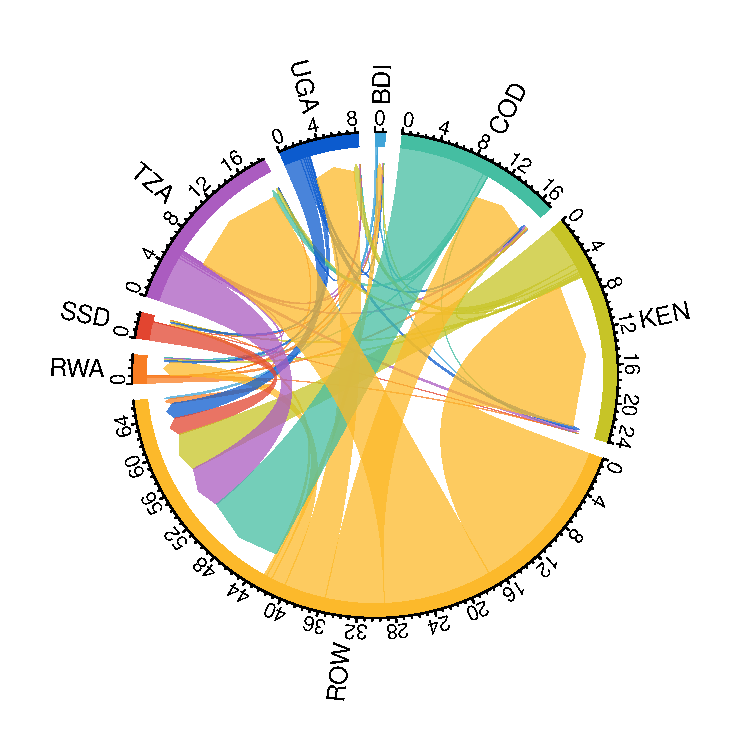
\includegraphics[width=0.4\textwidth, trim= {0.9cm 0.8cm 1.1cm 1cm}, clip]{"../Figures/REV/BACI_MIG_2010_19_ROW.pdf"} & %trim={<left> <lower> <right> <upper>}
%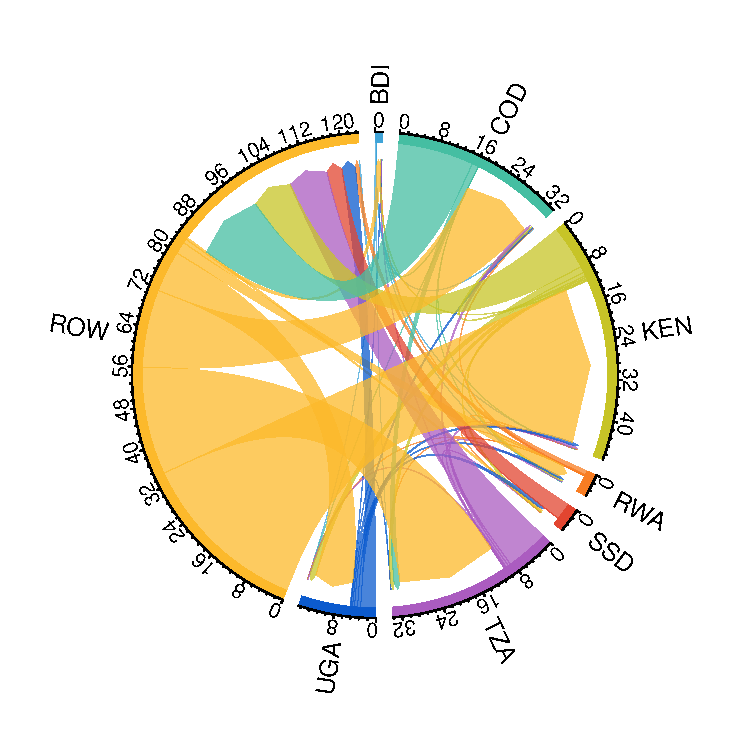
\includegraphics[width=0.4\textwidth, trim= {0.8cm 0.8cm 1cm 1cm}, clip]{"../Figures/REV/DOT_MIG_2010_19_ROW.pdf"} &
%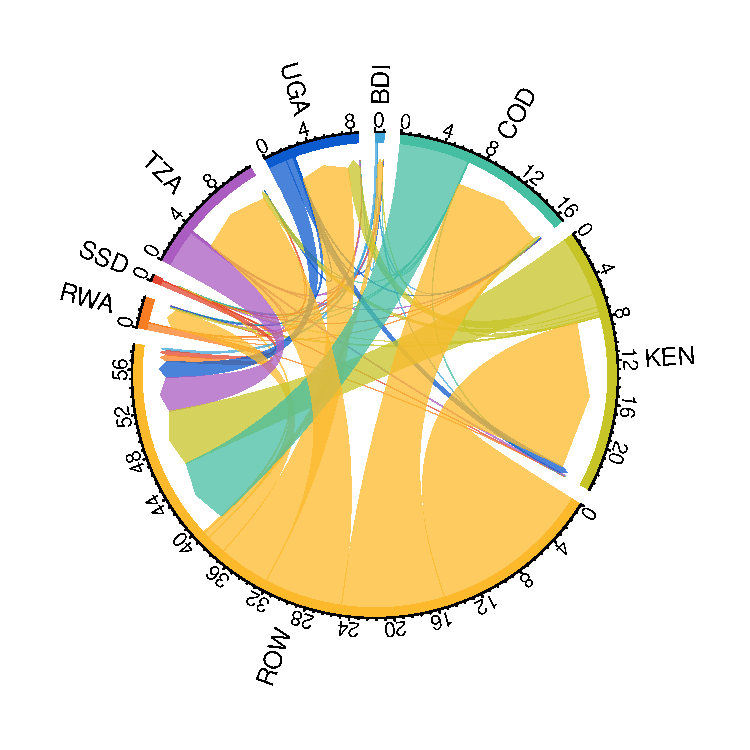
\includegraphics[width=0.4\textwidth, trim= {1cm 0.8cm 1cm 1cm}, clip]{"../Figures/REV/EORA_MIG_2010_19_ROW.pdf"} 
%\end{tabular}
%\end{adjustbox}
%\end{figure}
%\FloatBarrier

\begin{figure}[h!] \vspace{-1mm}
\centering
\caption{\label{fig:MIG_SEC_EORA}\textsc{Average Trade Flows by Broad Sector, 2010-2015: EORA: USD Billions}}
\vspace{2mm}
\resizebox{\textwidth}{!}{
\begin{tabular}{ccc}
Agriculture \& Livestock & Foods \& Beverages & Manufactured Goods \\
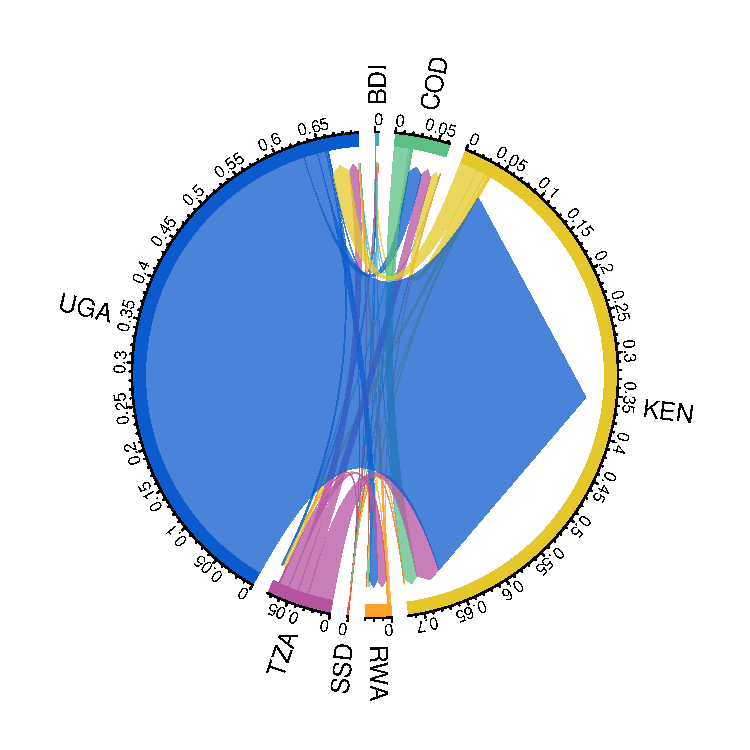
\includegraphics[width=0.4\textwidth, trim= {1.3cm 0.8cm 1.1cm 1cm}, clip]{"../Figures/REV/EORA_MIG_AGR_2010_19.pdf"} & %trim={<left> <lower> <right> <upper>}
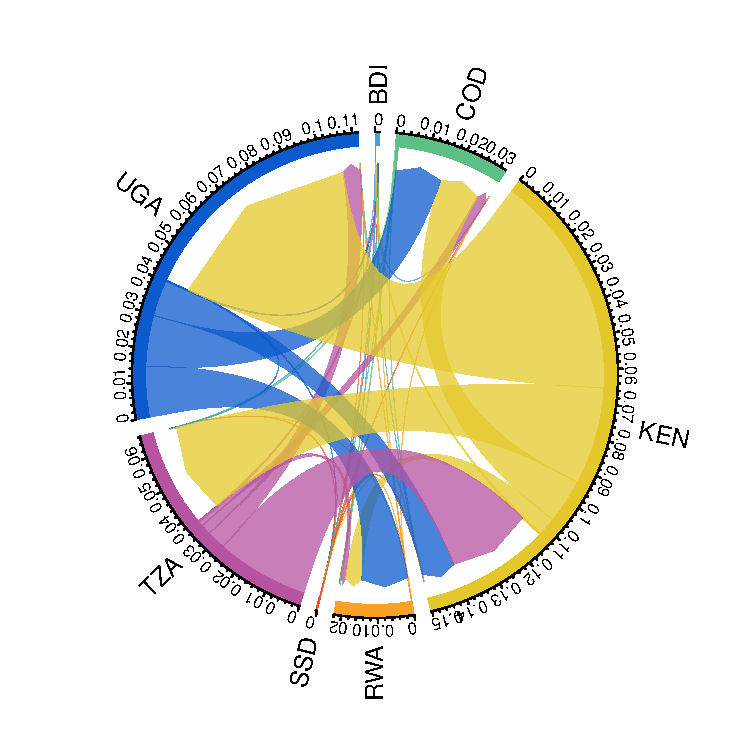
\includegraphics[width=0.4\textwidth, trim= {1.3cm 0.8cm 1.1cm 1cm}, clip]{"../Figures/REV/EORA_MIG_FBE_2010_19.pdf"} &
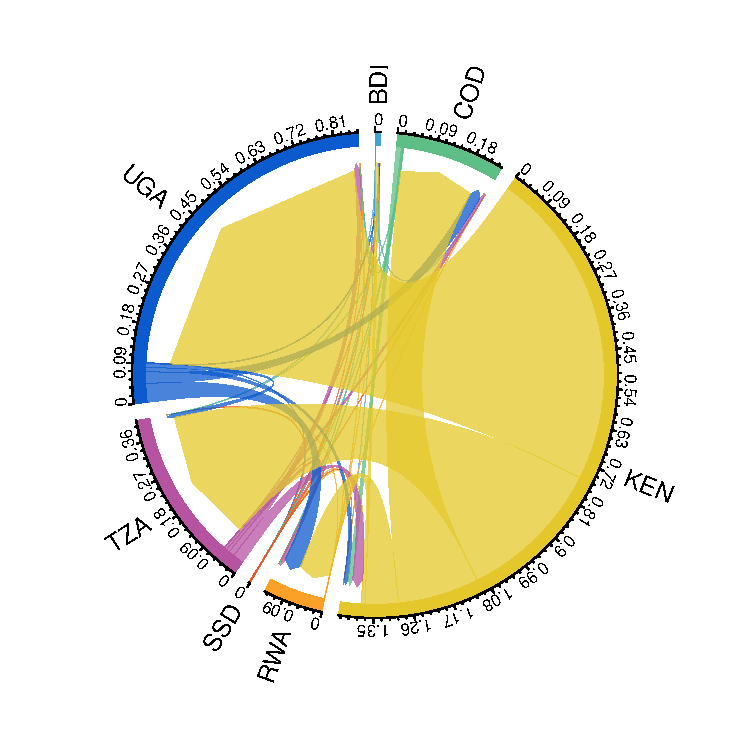
\includegraphics[width=0.4\textwidth, trim= {1.3cm 0.8cm 1.1cm 1cm}, clip]{"../Figures/REV/EORA_MIG_MAN_2010_19.pdf"} \\
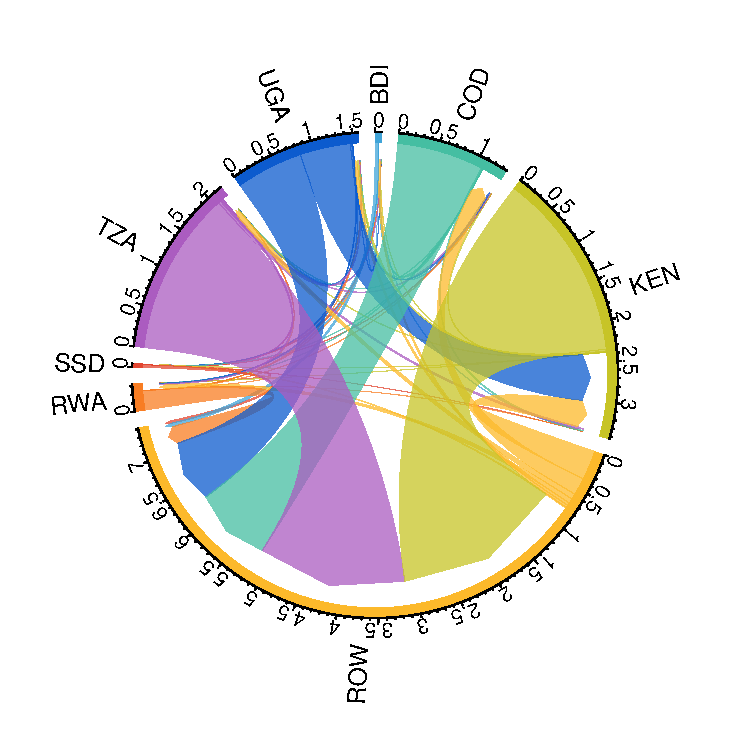
\includegraphics[width=0.4\textwidth, trim= {1.3cm 0.8cm 1.1cm 1cm}, clip]{"../Figures/REV/EORA_MIG_AGR_2010_19_ROW.pdf"} & %trim={<left> <lower> <right> <upper>}
\includegraphics[width=0.4\textwidth, trim= {1.3cm 0.8cm 1.1cm 1cm}, clip]{"../Figures/REV/EORA_MIG_FBE_2010_19_ROW.pdf"} &
\includegraphics[width=0.4\textwidth, trim= {1.3cm 0.8cm 1.1cm 1cm}, clip]{"../Figures/REV/EORA_MIG_MAN_2010_19_ROW.pdf"} \\
\end{tabular}
}
\end{figure}
\FloatBarrier


\begin{figure}[h!] \vspace{-1mm}
\centering
\caption{\label{fig:MIG_SEC_EM}\textsc{Average Trade Flows by Broad Sector, 2010-2015: EMERGING: USD Billions}}
\vspace{2mm}
\resizebox{\textwidth}{!}{
\begin{tabular}{ccc}
Agriculture \& Livestock & Foods \& Beverages & Manufactured Goods \\
\includegraphics[width=0.4\textwidth, trim= {1.3cm 0.8cm 1.1cm 1cm}, clip]{"../Figures/REV/EM_MIG_AGR_2010_19.pdf"} & %trim={<left> <lower> <right> <upper>}
\includegraphics[width=0.4\textwidth, trim= {1.3cm 0.8cm 1.1cm 1cm}, clip]{"../Figures/REV/EM_MIG_FBE_2010_19.pdf"} &
\includegraphics[width=0.4\textwidth, trim= {1.3cm 0.8cm 1.1cm 1cm}, clip]{"../Figures/REV/EM_MIG_MAN_2010_19.pdf"} \\
\includegraphics[width=0.4\textwidth, trim= {1.3cm 0.8cm 1.1cm 1cm}, clip]{"../Figures/REV/EM_MIG_AGR_2010_19_ROW.pdf"} & %trim={<left> <lower> <right> <upper>}
\includegraphics[width=0.4\textwidth, trim= {1.3cm 0.8cm 1.1cm 1cm}, clip]{"../Figures/REV/EM_MIG_FBE_2010_19_ROW.pdf"} &
\includegraphics[width=0.4\textwidth, trim= {1.3cm 0.8cm 1.1cm 1cm}, clip]{"../Figures/REV/EM_MIG_MAN_2010_19_ROW.pdf"} \\
\end{tabular}
}
\end{figure}
\FloatBarrier


% latex table generated in R 4.3.0 by xtable 1.8-4 package
% Mon Jan  8 22:03:44 2024
\begin{table}[ht]
\centering
  \caption{\label{tab:weaclfl}\textsc{Largest 50 Intermediate EAC Trade Flows: EMERGING 2015-19 Average}} 
  \small{\textit{Millions of Current USD at Basic Prices}}
\begin{tabular}{rllrllr}
  \toprule
 & \multicolumn{3}{c}{Overall} & \multicolumn{3}{c}{Inner-EAC} \\
 & From & To & Value & From & To & Value \\ 
  \midrule
  2 & UGA.PCM & MEA.MIN & 254.72 & KEN.PCM & UGA.CON & 65.28 \\ 
  3 & MEA.PCM & KEN.FBE & 245.28 & KEN.PCM & RWA.AFF & 41.38 \\ 
  4 & SAS.PCM & TZA.TRA & 244.89 & KEN.PCM & UGA.FBE & 40.42 \\ 
  5 & SAS.PCM & KEN.FBE & 233.83 & UGA.FBE & KEN.TRA & 40.12 \\ 
  6 & CHN.TEX & TZA.TEX & 222.33 & UGA.FBE & KEN.FBE & 38.88 \\ 
  7 & CHN.TEX & KEN.TEX & 213.58 & TZA.PCM & RWA.AFF & 38.36 \\ 
  8 & CHN.PCM & KEN.PCM & 213.41 & UGA.PCM & RWA.AFF & 31.44 \\ 
  9 & CHN.ELM & TZA.ELM & 211.46 & KEN.MPR & UGA.CON & 31.15 \\ 
  10 & CHN.TEX & KEN.TRA & 211.10 & TZA.AFF & KEN.FBE & 30.07 \\ 
  11 & KEN.TRA & EUU.TRA & 207.65 & KEN.FBE & UGA.FBE & 29.40 \\ 
  12 & TZA.PCM & ECA.PCM & 196.53 & KEN.PCM & UGA.AFF & 29.18 \\ 
  13 & KEN.FBE & SAS.FBE & 196.09 & UGA.AFF & KEN.FBE & 28.80 \\ 
  14 & KEN.AFF & EUU.FBE & 191.72 & KEN.PCM & TZA.PCM & 27.12 \\ 
  15 & MEA.PCM & TZA.TRA & 191.05 & KEN.MPR & UGA.MPR & 22.62 \\ 
  16 & CHN.MPR & KEN.EGW & 186.79 & RWA.FBE & KEN.FBE & 21.90 \\ 
  17 & UGA.PCM & MEA.CON & 180.61 & TZA.TEX & KEN.TEX & 19.46 \\ 
  18 & CHN.TEX & KEN.WAP & 175.45 & RWA.FBE & KEN.TRA & 17.37 \\ 
  19 & SAS.PCM & KEN.PCM & 172.61 & UGA.EGW & KEN.CON & 17.14 \\ 
  20 & TZA.AFF & SAS.AFF & 163.76 & UGA.PCM & RWA.TRA & 16.29 \\ 
  21 & KEN.AFF & EUU.AFF & 160.71 & KEN.FBE & UGA.SMH & 14.99 \\ 
  22 & CHN.PCM & KEN.FBE & 158.19 & UGA.AFF & KEN.AFF & 14.28 \\ 
  23 & SAS.PCM & KEN.EGW & 156.87 & KEN.MPR & UGA.PTE & 13.76 \\ 
  24 & TZA.PCM & SSA.MPR & 155.21 & TZA.WAP & KEN.WAP & 13.70 \\ 
  25 & MEA.PCM & KEN.PCM & 142.64 & TZA.FBE & KEN.TEX & 13.64 \\ 
  26 & MEA.PCM & KEN.EGW & 142.53 & KEN.PCM & TZA.FBE & 13.10 \\ 
  27 & CHN.PCM & TZA.CON & 136.05 & UGA.FBE & RWA.TRA & 13.07 \\ 
  28 & CHN.PCM & TZA.PCM & 135.90 & KEN.AFF & UGA.FBE & 12.36 \\ 
  29 & TZA.TRA & EUU.TRA & 131.02 & UGA.FBE & KEN.TEX & 12.33 \\ 
  30 & KEN.FBE & SAS.PCM & 129.12 & KEN.PCM & UGA.TRA & 12.22 \\ 
  31 & UGA.PCM & MEA.PCM & 129.11 & KEN.PCM & UGA.EGW & 11.55 \\ 
  32 & MEA.PCM & KEN.CON & 128.95 & UGA.WAP & KEN.WAP & 11.23 \\ 
  33 & EUU.PCM & KEN.PCM & 114.90 & KEN.TEX & UGA.TEX & 10.58 \\ 
  34 & CHN.PCM & KEN.AFF & 114.73 & TZA.FBE & KEN.FBE & 10.45 \\ 
  35 & SAS.PCM & KEN.AFF & 113.57 & TZA.FBE & KEN.PCM & 10.21 \\ 
  36 & EUU.PCM & KEN.FBE & 113.21 & TZA.WAP & KEN.FBE & 9.72 \\ 
  37 & CHN.ELM & TZA.CON & 113.02 & UGA.FBE & KEN.PCM & 8.79 \\ 
  38 & CHN.ELM & UGA.EGW & 112.73 & UGA.WAP & KEN.FBE & 8.42 \\ 
  39 & MEA.PCM & TZA.CON & 106.08 & KEN.PCM & RWA.FBE & 8.40 \\ 
  40 & KEN.FBE & MEA.FBE & 104.53 & TZA.TEX & KEN.TRA & 8.00 \\ 
  41 & CHN.MAN & KEN.MAN & 104.29 & KEN.PCM & BDI.AFF & 8.00 \\ 
  42 & UGA.FBE & EUU.FBE & 102.62 & KEN.FBE & UGA.TRA & 7.66 \\ 
  43 & TZA.AFF & ASE.AFF & 102.24 & TZA.FBE & KEN.TRA & 7.18 \\ 
  44 & CHN.ELM & KEN.CON & 100.89 & TZA.AFF & KEN.AFF & 6.96 \\ 
  45 & CHN.MPR & TZA.ELM & 98.29 & KEN.PCM & TZA.CON & 6.93 \\ 
  46 & KEN.FBE & EUU.FBE & 96.18 & KEN.PCM & TZA.TRA & 6.83 \\ 
  47 & TZA.PCM & SSA.PCM & 95.74 & TZA.PCM & BDI.AFF & 6.80 \\ 
  48 & CHN.ELM & KEN.FBE & 94.59 & KEN.FBE & UGA.PTE & 6.49 \\ 
  49 & SAS.PCM & KEN.CON & 93.59 & KEN.PCM & TZA.AFF & 6.48 \\ 
  50 & TZA.TRA & SAS.TRA & 91.13 & KEN.WAP & RWA.CON & 6.43 \\ 
   \bottomrule
\end{tabular}
\end{table}


\begin{figure}[h!] \vspace{-3mm}
\centering
\caption{\label{fig:exp_EAC_share}\textsc{Percentage of Gross Exports Going to EAC Members}}
\includegraphics[width=1\textwidth, trim= {0 0 0 0}, clip]{"../Figures/exports_EAC_perc_stacked_ts".pdf} %trim={<left> <lower> <right> <upper>}
\end{figure}
\FloatBarrier

%\begin{figure}[!h]
%\centering
%\vspace{-2cm}
%\caption{\label{fig:outshares}\textsc{Decomposition of Sectoral Output and Exports}}
%\vspace*{\fill}
%\begin{adjustbox}{center}
%\includegraphics[width=1.75\textwidth, angle =270, trim= {1cm 0 0 0}, clip]{"../Figures/output_shares".pdf} %trim={<left> <lower> <right> <upper>}
%\end{adjustbox}
%\vspace*{\fill}
%\end{figure}
%\FloatBarrier


\begin{figure}[h!] % \vspace{-2mm}
\centering
\caption{\label{fig:KWW}\textsc{Refined Koopman Wang Wei Decomposition of Gross Exports}}
\includegraphics[width=1\textwidth, trim= {0 0 0 0}, clip]{"../Figures/REV/KWW_DEC_NEW.png"} %trim={<left> <lower> <right> <upper>}
\raggedleft
\scriptsize
\emph{Source:} \citet{antras2022global}
% \vspace{-1cm}
\end{figure}
\FloatBarrier

\begin{figure}[h!]
\centering
\caption{\label{fig:KWW_fill_ts}\textsc{KWW Decomposition of Gross Exports}}
\includegraphics[width=1\textwidth]{"../Figures/REV/KWW_DEC_NEW.pdf"} %trim={<left> <lower> <right> <upper>}
% \vspace{-1cm}
\end{figure}
\FloatBarrier





% latex table generated in R 4.3.0 by xtable 1.8-4 package
% Thu Jan 18 10:17:19 2024
\begin{table}[ht]
\centering
\caption{\label{tab:NRCA} (N)RCA Estimates from Figure \ref{fig:NRCA}}
\vspace{2mm}
\resizebox{\textwidth}{!}{
\begin{tabular}{lllrrrrrrrrrrrrrrrrr}
  \toprule
Country & Source & Flow & AFF & MIN & FBE & TEX & WAP & PCM & MPR & ELM & TEQ & MAN & EGW & CON & SMH & TRA & PTE & FIB & PAO \\ 
  \midrule
UGA & WDR\_EORA & GX & 16.07 & 0.14 & 2.49 & 0.24 & 0.29 & 0.18 & 0.39 & 0.18 & 0.28 & 0.95 & 0.93 & 4.57 & 2.33 & 2.04 & 2.76 & 0.02 & 1.09 \\ 
  TZA & WDR\_EORA & GX & 10.48 & 1.48 & 2.42 & 1.63 & 0.57 & 0.21 & 0.20 & 0.12 & 0.29 & 4.58 & 3.99 & 2.03 & 1.15 & 1.06 & 1.43 & 1.02 & 0.58 \\ 
  KEN & WDR\_EORA & GX & 11.57 & 1.09 & 2.95 & 0.94 & 0.94 & 0.73 & 0.44 & 0.26 & 0.08 & 1.04 & 1.61 & 1.11 & 1.41 & 1.70 & 1.73 & 0.44 & 0.19 \\ 
  RWA & WDR\_EORA & GX & 4.40 & 4.49 & 0.29 & 0.29 & 0.35 & 0.16 & 0.32 & 0.11 & 0.10 & 0.67 & 4.86 & 9.81 & 4.05 & 1.69 & 5.12 & 0.12 & 2.55 \\ 
  BDI & WDR\_EORA & GX & 6.83 & 0.32 & 0.31 & 0.38 & 0.20 & 0.13 & 0.24 & 0.07 & 0.25 & 1.18 & 4.23 & 12.99 & 5.53 & 1.82 & 6.10 & 0.10 & 3.50 \\ 
  EAC5 & WDR\_EORA & GX & 11.54 & 1.10 & 2.68 & 0.96 & 0.77 & 0.55 & 0.38 & 0.22 & 0.14 & 1.64 & 2.09 & 2.17 & 1.64 & 1.63 & 2.00 & 0.48 & 0.50 \\ \midrule
  UGA & EORA & GX & 17.33 & 0.11 & 2.83 & 0.22 & 0.36 & 0.19 & 0.39 & 0.16 & 0.35 & 0.79 & 1.25 & 3.98 & 2.05 & 1.81 & 2.69 & 0.02 & 1.35 \\ 
  TZA & EORA & GX & 11.30 & 1.08 & 2.69 & 1.56 & 0.71 & 0.22 & 0.20 & 0.10 & 0.38 & 3.97 & 4.98 & 1.72 & 0.98 & 0.93 & 1.34 & 1.00 & 0.67 \\ 
  KEN & EORA & GX & 11.95 & 0.79 & 3.41 & 0.89 & 1.20 & 0.77 & 0.44 & 0.23 & 0.11 & 0.92 & 2.20 & 0.95 & 1.24 & 1.56 & 1.73 & 0.44 & 0.25 \\ 
  RWA & EORA & GX & 4.82 & 3.38 & 0.34 & 0.28 & 0.45 & 0.17 & 0.32 & 0.10 & 0.14 & 0.58 & 6.55 & 8.74 & 3.56 & 1.50 & 5.07 & 0.12 & 3.23 \\ 
  BDI & EORA & GX & 7.43 & 0.24 & 0.36 & 0.35 & 0.26 & 0.13 & 0.25 & 0.07 & 0.34 & 0.98 & 5.49 & 11.58 & 4.86 & 1.62 & 6.05 & 0.10 & 4.40 \\ 
  EAC5 & EORA & GX & 12.28 & 0.83 & 3.07 & 0.90 & 0.98 & 0.58 & 0.38 & 0.20 & 0.19 & 1.39 & 2.92 & 1.91 & 1.43 & 1.45 & 1.94 & 0.47 & 0.65 \\ \midrule
  UGA & EMERGING & GX & 4.76 & 0.00 & 7.16 & 0.52 & 0.70 & 0.82 & 0.46 & 0.03 & 0.05 & 0.14 & 7.29 & 0.19 & 4.42 & 1.92 & 0.03 & 0.16 & 0.12 \\ 
  TZA & EMERGING & GX & 4.93 & 0.01 & 2.46 & 0.55 & 0.64 & 1.38 & 0.58 & 0.04 & 0.04 & 0.12 & 0.00 & 1.61 & 3.04 & 3.41 & 0.27 & 0.02 & 0.06 \\ 
  KEN & EMERGING & GX & 4.16 & 0.01 & 5.98 & 1.01 & 0.94 & 0.55 & 0.47 & 0.06 & 0.10 & 0.33 & 1.17 & 0.00 & 2.17 & 3.28 & 0.29 & 0.13 & 6.78 \\ 
  RWA & EMERGING & GX & 0.74 & 0.00 & 5.11 & 0.24 & 0.07 & 1.41 & 0.17 & 0.05 & 0.06 & 0.10 & 0.69 & 0.51 & 5.67 & 2.00 & 0.02 & 0.01 & 2.26 \\ 
  BDI & EMERGING & GX & 0.16 & 0.00 & 10.83 & 0.31 & 0.06 & 0.95 & 0.22 & 0.04 & 0.08 & 0.07 & 0.00 & 0.01 & 0.02 & 1.30 & 0.12 & 0.01 & 24.16 \\ 
  EAC5 & EMERGING & GX & 4.12 & 0.01 & 5.12 & 0.70 & 0.77 & 0.90 & 0.49 & 0.06 & 0.08 & 0.21 & 2.09 & 0.61 & 3.08 & 2.90 & 0.21 & 0.09 & 3.16 \\ \midrule
  UGA & BACI & GX & 5.03 & 0.08 & 7.60 & 0.88 & 0.73 & 0.68 & 0.80 & 0.18 & 0.20 & 0.24 &  &  &  &  &  &  &  \\ 
  TZA & BACI & GX & 5.08 & 0.23 & 2.85 & 0.93 & 0.60 & 2.42 & 0.58 & 0.13 & 0.08 & 0.16 &  &  &  &  &  &  &  \\ 
  KEN & BACI & GX & 5.74 & 0.45 & 6.61 & 1.63 & 0.89 & 0.77 & 0.59 & 0.17 & 0.12 & 0.40 &  &  &  &  &  &  &  \\ 
  RWA & BACI & GX & 1.27 & 0.65 & 5.02 & 0.51 & 0.18 & 2.32 & 0.26 & 0.07 & 0.11 & 0.18 &  &  &  &  &  &  &  \\ 
  BDI & BACI & GX & 0.25 & 0.02 & 5.53 & 0.42 & 0.06 & 2.84 & 0.30 & 0.07 & 0.09 & 0.11 &  &  &  &  &  &  &  \\ 
  EAC5 & BACI & GX & 5.21 & 0.32 & 5.16 & 1.19 & 0.73 & 1.55 & 0.58 & 0.15 & 0.15 & 0.28 &  &  &  &  &  &  &  \\ \midrule
  UGA & WDR\_EORA & VAX & 13.87 & 0.11 & 2.24 & 0.20 & 0.25 & 0.16 & 0.33 & 0.15 & 0.24 & 0.82 & 0.78 & 4.02 & 1.94 & 1.79 & 2.37 & 0.02 & 3.42 \\ 
  TZA & WDR\_EORA & VAX & 10.87 & 1.23 & 2.07 & 1.31 & 0.42 & 0.16 & 0.13 & 0.07 & 0.15 & 3.15 & 3.76 & 1.75 & 1.01 & 0.91 & 1.39 & 1.04 & 1.76 \\ 
  KEN & WDR\_EORA & VAX & 10.62 & 0.84 & 2.63 & 0.91 & 0.84 & 0.72 & 0.29 & 0.19 & 0.06 & 0.98 & 1.52 & 0.86 & 1.22 & 1.42 & 1.53 & 0.38 & 0.64 \\ 
  RWA & WDR\_EORA & VAX & 4.55 & 3.74 & 0.31 & 0.24 & 0.35 & 0.17 & 0.30 & 0.11 & 0.09 & 0.27 & 4.23 & 10.26 & 3.49 & 1.70 & 5.07 & 0.11 & 4.19 \\ 
  BDI & WDR\_EORA & VAX & 6.36 & 0.19 & 0.31 & 0.30 & 0.20 & 0.13 & 0.23 & 0.08 & 0.26 & 0.82 & 3.41 & 12.58 & 4.41 & 1.72 & 5.43 & 0.09 & 9.87 \\ 
  EAC5 & WDR\_EORA & VAX & 10.80 & 0.86 & 2.38 & 0.85 & 0.68 & 0.54 & 0.27 & 0.16 & 0.10 & 1.24 & 1.87 & 1.91 & 1.42 & 1.41 & 1.80 & 0.42 & 1.44 \\ \midrule
  UGA & EORA & VAX & 16.59 & 0.10 & 2.57 & 0.19 & 0.32 & 0.16 & 0.34 & 0.14 & 0.28 & 0.71 & 1.19 & 3.72 & 1.92 & 1.73 & 2.55 & 0.02 & 1.57 \\ 
  TZA & EORA & VAX & 13.12 & 1.06 & 2.19 & 1.24 & 0.52 & 0.15 & 0.12 & 0.06 & 0.16 & 2.74 & 5.25 & 1.53 & 0.95 & 0.85 & 1.40 & 1.12 & 0.75 \\ 
  KEN & EORA & VAX & 12.20 & 0.72 & 3.07 & 0.89 & 1.09 & 0.75 & 0.30 & 0.17 & 0.07 & 0.90 & 2.32 & 0.80 & 1.21 & 1.41 & 1.69 & 0.43 & 0.32 \\ 
  RWA & EORA & VAX & 5.37 & 3.29 & 0.37 & 0.23 & 0.46 & 0.18 & 0.30 & 0.10 & 0.12 & 0.26 & 6.42 & 9.69 & 3.43 & 1.65 & 5.46 & 0.13 & 2.10 \\ 
  BDI & EORA & VAX & 7.67 & 0.17 & 0.37 & 0.29 & 0.26 & 0.14 & 0.25 & 0.08 & 0.32 & 0.75 & 4.96 & 12.92 & 4.37 & 1.68 & 5.95 & 0.11 & 4.75 \\ 
  EAC5 & EORA & VAX & 12.68 & 0.76 & 2.76 & 0.83 & 0.88 & 0.56 & 0.28 & 0.14 & 0.12 & 1.10 & 2.97 & 1.78 & 1.39 & 1.35 & 1.93 & 0.47 & 0.72 \\ \midrule
  UGA & EMERGING & VAX & 4.67 & 0.00 & 6.15 & 0.42 & 0.65 & 0.79 & 0.40 & 0.03 & 0.05 & 0.12 & 5.87 & 0.18 & 4.36 & 1.92 & 0.02 & 0.16 & 0.11 \\ 
  TZA & EMERGING & VAX & 5.08 & 0.01 & 2.53 & 0.55 & 0.58 & 1.43 & 0.51 & 0.03 & 0.04 & 0.10 & 0.00 & 1.58 & 2.83 & 3.02 & 0.23 & 0.02 & 0.06 \\ 
  KEN & EMERGING & VAX & 4.05 & 0.01 & 5.79 & 0.84 & 0.60 & 0.52 & 0.47 & 0.05 & 0.07 & 0.26 & 0.99 & 0.00 & 2.00 & 3.13 & 0.27 & 0.13 & 6.02 \\ 
  RWA & EMERGING & VAX & 0.77 & 0.00 & 4.50 & 0.26 & 0.08 & 1.56 & 0.18 & 0.06 & 0.08 & 0.11 & 0.79 & 0.52 & 4.64 & 2.06 & 0.02 & 0.01 & 2.30 \\ 
  BDI & EMERGING & VAX & 0.16 & 0.00 & 9.67 & 0.34 & 0.06 & 0.69 & 0.18 & 0.04 & 0.07 & 0.09 & 0.00 & 0.01 & 0.02 & 1.47 & 0.13 & 0.01 & 26.19 \\ 
  EAC5 & EMERGING & VAX & 4.17 & 0.01 & 5.01 & 0.61 & 0.58 & 0.89 & 0.43 & 0.05 & 0.08 & 0.18 & 1.73 & 0.58 & 2.85 & 2.77 & 0.19 & 0.09 & 2.91 \\ 
   \bottomrule
\end{tabular}
}
\end{table}


% latex table generated in R 4.3.0 by xtable 1.8-4 package
% Wed Jan 17 22:19:44 2024
\begin{table}[ht]
\centering
\caption{\label{tab:NRCA_corr}\textsc{(New) Revealed Comparative Advantage: Correlations of 2010-19 Medians}}
\vspace{2mm}
\begin{tabular}{lrrrrrrr}
  \toprule
  & \multicolumn{2}{c}{WDR EORA} & \multicolumn{2}{c}{EORA} & \multicolumn{2}{c}{EMERGING} & BACI \\
 & GX & VAX & GX & VAX & GX & VAX & GX \\ 
  \midrule
  WDR\_EORA\_GX &    1   &  .962 &  .990 &  .987 &  .179 &  .186 &  .550 \\ 
  WDR\_EORA\_VAX &  .962 &    1   &  .960 &  .967 &  .341 &  .362 &  .563 \\ 
  EORA\_GX &  .990 &  .960 &    1   &  .995 &  .215 &  .223 &  .571 \\ 
  EORA\_VAX &  .987 &  .967 &  .995 &    1   &  .217 &  .227 &  .570 \\ 
  EMERGING\_GX &  .179 &  .341 &  .215 &  .217 &    1   &  .994 &  .925 \\ 
  EMERGING\_VAX &  .186 &  .362 &  .223 &  .227 &  .994 &    1   &  .934 \\ 
  BACI\_GX &  .550 &  .563 &  .571 &  .570 &  .925 &  .934 &    1   \\ 
   \bottomrule \\ [-0.9em]
\multicolumn{8}{l}{\parbox{0.7\textwidth}{\scriptsize
\textit{Notes:} WDR EORA is only available for 2010-15, EMERGING misses years 2011-14.}}
\end{tabular}
\end{table}


% latex table generated in R 4.3.0 by xtable 1.8-4 package
% Thu Jan 18 10:17:19 2024
\begin{table}[ht]
\centering
\caption{\label{tab:EAC_NRCA} (N)RCA Estimates from Figure \ref{fig:EAC_NRCA}}
\vspace{2mm}
\resizebox{\textwidth}{!}{
\begin{tabular}{lllrrrrrrrrrrrrrrrrr}
  \toprule
Country & Source & Flow & AFF & MIN & FBE & TEX & WAP & PCM & MPR & ELM & TEQ & MAN & EGW & CON & SMH & TRA & PTE & FIB & PAO \\ 
  \midrule
 \multicolumn{10}{l}{Relative to the EAC} \\ \midrule
  UGA & WDR\_EORA & GX & 1.39 & 0.13 & 0.93 & 0.26 & 0.38 & 0.33 & 1.02 & 0.81 & 1.95 & 0.58 & 0.43 & 2.12 & 1.41 & 1.25 & 1.37 & 0.05 & 2.17 \\ 
  TZA & WDR\_EORA & GX & 0.91 & 1.32 & 0.91 & 1.71 & 0.74 & 0.38 & 0.52 & 0.54 & 2.04 & 2.80 & 1.90 & 0.93 & 0.70 & 0.65 & 0.71 & 2.12 & 1.16 \\ 
  KEN & WDR\_EORA & GX & 1.00 & 0.98 & 1.10 & 0.99 & 1.22 & 1.32 & 1.14 & 1.19 & 0.56 & 0.64 & 0.77 & 0.51 & 0.87 & 1.04 & 0.88 & 0.92 & 0.38 \\ 
  RWA & WDR\_EORA & GX & 0.39 & 4.06 & 0.11 & 0.30 & 0.45 & 0.29 & 0.84 & 0.50 & 0.69 & 0.40 & 2.35 & 4.57 & 2.47 & 1.04 & 2.56 & 0.24 & 5.20 \\ 
  BDI & WDR\_EORA & GX & 0.60 & 0.29 & 0.12 & 0.39 & 0.26 & 0.23 & 0.64 & 0.34 & 1.73 & 0.71 & 2.01 & 6.05 & 3.38 & 1.12 & 3.07 & 0.21 & 7.14 \\ \midrule
  UGA & EORA & GX & 1.34 & 0.13 & 0.91 & 0.26 & 0.39 & 0.32 & 1.03 & 0.80 & 1.88 & 0.57 & 0.45 & 2.06 & 1.40 & 1.24 & 1.36 & 0.05 & 2.10 \\ 
  TZA & EORA & GX & 0.92 & 1.25 & 0.87 & 1.68 & 0.72 & 0.37 & 0.50 & 0.52 & 2.02 & 2.76 & 1.83 & 0.90 & 0.68 & 0.64 & 0.69 & 2.12 & 1.11 \\ 
  KEN & EORA & GX & 0.99 & 1.00 & 1.12 & 0.99 & 1.23 & 1.33 & 1.15 & 1.20 & 0.58 & 0.64 & 0.79 & 0.54 & 0.88 & 1.05 & 0.89 & 0.94 & 0.40 \\ 
  RWA & EORA & GX & 0.40 & 3.96 & 0.11 & 0.31 & 0.46 & 0.30 & 0.86 & 0.50 & 0.72 & 0.41 & 2.24 & 4.48 & 2.46 & 1.01 & 2.55 & 0.24 & 5.02 \\ 
  BDI & EORA & GX & 0.59 & 0.28 & 0.12 & 0.40 & 0.27 & 0.23 & 0.65 & 0.34 & 1.78 & 0.73 & 1.94 & 6.26 & 3.42 & 1.09 & 3.03 & 0.22 & 6.88 \\ \midrule
  UGA & EMERGING & GX & 1.02 & 0.07 & 1.43 & 0.74 & 0.82 & 0.82 & 0.85 & 0.47 & 0.70 & 0.51 & 4.06 & 0.31 & 1.40 & 0.65 & 0.13 & 1.71 & 0.04 \\ 
  TZA & EMERGING & GX & 1.12 & 1.83 & 0.56 & 0.80 & 1.08 & 1.48 & 1.14 & 0.73 & 0.50 & 0.59 & 0.00 & 2.71 & 0.97 & 1.17 & 1.27 & 0.22 & 0.02 \\ 
  KEN & EMERGING & GX & 1.04 & 0.81 & 1.18 & 1.46 & 1.08 & 0.63 & 1.02 & 1.30 & 1.34 & 1.52 & 0.54 & 0.00 & 0.71 & 1.11 & 1.36 & 1.42 & 2.14 \\ 
  RWA & EMERGING & GX & 0.18 & 0.17 & 1.02 & 0.31 & 0.10 & 1.34 & 0.34 & 0.77 & 0.70 & 0.30 & 0.33 & 0.81 & 1.88 & 0.69 & 0.07 & 0.14 & 0.74 \\ 
  BDI & EMERGING & GX & 0.04 & 0.13 & 2.08 & 0.42 & 0.07 & 1.03 & 0.44 & 0.72 & 0.95 & 0.38 & 0.00 & 0.02 & 0.01 & 0.46 & 0.51 & 0.14 & 7.64 \\ \midrule
  UGA & BACI & GX & 0.97 & 0.29 & 1.43 & 0.78 & 0.96 & 0.44 & 1.21 & 1.14 & 1.87 & 0.89 &  &  &  &  &  &  &  \\ 
  TZA & BACI & GX & 0.97 & 0.65 & 0.53 & 0.75 & 0.87 & 1.57 & 0.97 & 0.83 & 0.51 & 0.63 &  &  &  &  &  &  &  \\ 
  KEN & BACI & GX & 1.13 & 1.49 & 1.28 & 1.42 & 1.28 & 0.48 & 0.99 & 1.16 & 0.98 & 1.43 &  &  &  &  &  &  &  \\ 
  RWA & BACI & GX & 0.25 & 1.95 & 1.00 & 0.42 & 0.24 & 1.44 & 0.48 & 0.52 & 0.89 & 0.67 &  &  &  &  &  &  &  \\ 
  BDI & BACI & GX & 0.05 & 0.09 & 1.17 & 0.35 & 0.07 & 1.70 & 0.43 & 0.56 & 0.78 & 0.39 &  &  &  &  &  &  &  \\ \midrule
  UGA & WDR\_EORA & VAX & 1.28 & 0.13 & 0.94 & 0.24 & 0.37 & 0.29 & 1.22 & 0.97 & 2.38 & 0.65 & 0.41 & 2.13 & 1.35 & 1.27 & 1.30 & 0.04 & 2.28 \\ 
  TZA & WDR\_EORA & VAX & 1.01 & 1.43 & 0.87 & 1.51 & 0.61 & 0.29 & 0.45 & 0.43 & 1.48 & 2.51 & 2.02 & 0.92 & 0.70 & 0.64 & 0.77 & 2.48 & 1.23 \\ 
  KEN & WDR\_EORA & VAX & 0.98 & 0.98 & 1.10 & 1.07 & 1.24 & 1.32 & 1.08 & 1.16 & 0.60 & 0.78 & 0.81 & 0.46 & 0.87 & 1.02 & 0.86 & 0.90 & 0.44 \\ 
  RWA & WDR\_EORA & VAX & 0.42 & 4.33 & 0.13 & 0.28 & 0.51 & 0.32 & 1.10 & 0.69 & 0.93 & 0.21 & 2.29 & 5.48 & 2.46 & 1.21 & 2.81 & 0.27 & 2.75 \\ 
  BDI & WDR\_EORA & VAX & 0.60 & 0.22 & 0.13 & 0.35 & 0.29 & 0.25 & 0.85 & 0.50 & 2.57 & 0.65 & 1.82 & 6.74 & 3.11 & 1.22 & 3.03 & 0.22 & 6.76 \\ \midrule
  UGA & EORA & VAX & 1.28 & 0.13 & 0.92 & 0.23 & 0.38 & 0.29 & 1.16 & 0.93 & 2.16 & 0.61 & 0.42 & 2.06 & 1.34 & 1.26 & 1.29 & 0.05 & 2.21 \\ 
  TZA & EORA & VAX & 1.03 & 1.36 & 0.79 & 1.49 & 0.59 & 0.27 & 0.45 & 0.41 & 1.31 & 2.46 & 1.93 & 0.86 & 0.68 & 0.63 & 0.73 & 2.35 & 1.12 \\ 
  KEN & EORA & VAX & 0.97 & 1.00 & 1.12 & 1.09 & 1.25 & 1.33 & 1.10 & 1.17 & 0.61 & 0.80 & 0.84 & 0.48 & 0.89 & 1.02 & 0.87 & 0.92 & 0.47 \\ 
  RWA & EORA & VAX & 0.44 & 4.28 & 0.13 & 0.29 & 0.52 & 0.32 & 1.05 & 0.68 & 0.95 & 0.23 & 2.27 & 5.30 & 2.43 & 1.20 & 2.77 & 0.27 & 2.75 \\ 
  BDI & EORA & VAX & 0.62 & 0.22 & 0.13 & 0.33 & 0.29 & 0.25 & 0.87 & 0.51 & 2.64 & 0.65 & 1.74 & 6.94 & 3.19 & 1.21 & 3.13 & 0.23 & 6.76 \\ \midrule
  UGA & EMERGING & VAX & 1.05 & 0.06 & 1.26 & 0.71 & 1.09 & 0.80 & 0.80 & 0.66 & 0.87 & 0.53 & 3.98 & 0.31 & 1.50 & 0.67 & 0.13 & 1.73 & 0.04 \\ 
  TZA & EMERGING & VAX & 1.15 & 1.89 & 0.60 & 0.87 & 1.21 & 1.53 & 1.12 & 0.71 & 0.57 & 0.62 & 0.00 & 2.86 & 0.97 & 1.09 & 1.15 & 0.21 & 0.02 \\ 
  KEN & EMERGING & VAX & 1.00 & 0.80 & 1.24 & 1.37 & 0.91 & 0.58 & 1.00 & 1.19 & 1.07 & 1.43 & 0.52 & 0.00 & 0.70 & 1.13 & 1.41 & 1.37 & 2.05 \\ 
  RWA & EMERGING & VAX & 0.19 & 0.19 & 0.93 & 0.37 & 0.15 & 1.60 & 0.41 & 1.03 & 0.88 & 0.42 & 0.44 & 0.88 & 1.63 & 0.75 & 0.09 & 0.15 & 0.80 \\ 
  BDI & EMERGING & VAX & 0.04 & 0.11 & 2.06 & 0.53 & 0.10 & 0.75 & 0.41 & 0.76 & 0.86 & 0.57 & 0.00 & 0.03 & 0.01 & 0.54 & 0.63 & 0.15 & 8.59 \\ \midrule
  
   \multicolumn{10}{l}{In Inner-EAC Trade} \\ \midrule
  UGA & EORA & GX & 5.74 & 0.02 & 0.89 & 0.18 & 0.21 & 0.25 & 0.41 & 0.33 & 1.26 & 0.47 & 0.07 & 0.94 & 0.71 & 0.85 & 0.64 & 0.00 & 2.13 \\ 
  TZA & EORA & GX & 1.14 & 0.37 & 3.74 & 0.92 & 0.49 & 0.38 & 0.24 & 0.71 & 1.49 & 2.81 & 1.62 & 0.98 & 0.63 & 0.85 & 0.90 & 2.88 & 2.64 \\ 
  KEN & EORA & GX & 0.13 & 1.22 & 0.86 & 1.15 & 1.18 & 1.18 & 1.15 & 1.14 & 0.93 & 0.98 & 1.11 & 0.94 & 1.06 & 1.03 & 1.06 & 1.07 & 0.66 \\ 
  RWA & EORA & GX & 1.64 & 0.33 & 0.66 & 0.43 & 0.24 & 0.36 & 0.43 & 0.38 & 0.75 & 0.54 & 7.71 & 15.20 & 3.40 & 1.41 & 3.10 & 0.45 & 15.32 \\ 
  BDI & EORA & GX & 1.09 & 0.23 & 0.35 & 0.42 & 0.13 & 0.12 & 0.33 & 0.18 & 1.83 & 1.13 & 7.06 & 27.72 & 4.85 & 0.73 & 4.00 & 0.44 & 24.83 \\ \midrule
  UGA & EMERGING & GX & 2.04 & 0.01 & 1.61 & 0.51 & 1.18 & 0.53 & 0.95 & 0.16 & 0.17 & 0.33 & 2.78 & 0.00 & 0.40 & 0.85 & 0.98 & 2.47 & 0.06 \\ 
  TZA & EMERGING & GX & 1.47 & 2.92 & 0.61 & 1.90 & 1.38 & 0.75 & 0.48 & 0.84 & 0.29 & 0.19 &  & 4.11 & 0.64 & 1.34 & 1.87 & 0.09 & 0.01 \\ 
  KEN & EMERGING & GX & 0.28 & 0.70 & 0.72 & 0.99 & 0.93 & 1.52 & 1.34 & 1.37 & 1.79 & 1.63 & 0.47 & 0.00 & 1.60 & 1.01 & 0.74 & 0.64 & 0.56 \\ 
  RWA & EMERGING & GX & 0.87 & 0.64 & 2.00 & 1.38 & 0.06 & 0.49 & 0.19 & 0.88 & 0.53 & 0.46 & 0.51 & 0.00 & 0.84 & 0.25 & 0.02 & 0.05 & 13.67 \\ 
  BDI & EMERGING & GX & 0.24 & 0.15 & 2.11 & 0.99 & 0.12 & 0.57 & 0.65 & 0.95 & 0.84 & 0.60 & 0.00 & 0.00 & 0.05 & 0.94 & 1.26 & 0.20 & 21.95 \\  \midrule
  UGA & BACI & GX & 1.67 & 0.52 & 1.70 & 0.44 & 0.89 & 0.66 & 1.04 & 0.70 & 0.55 & 0.28 &  &  &  &  &  &  &  \\ 
  TZA & BACI & GX & 2.07 & 0.94 & 0.58 & 1.83 & 1.36 & 0.84 & 0.50 & 0.59 & 0.70 & 0.63 &  &  &  &  &  &  &  \\ 
  KEN & BACI & GX & 0.24 & 1.10 & 0.76 & 0.92 & 0.97 & 1.32 & 1.23 & 1.25 & 1.31 & 1.48 &  &  &  &  &  &  &  \\ 
  RWA & BACI & GX & 0.50 & 1.07 & 2.08 & 1.96 & 0.11 & 0.21 & 0.58 & 0.73 & 1.04 & 0.55 &  &  &  &  &  &  &  \\ 
  BDI & BACI & GX & 0.44 & 0.03 & 1.24 & 0.97 & 0.15 & 0.61 & 1.33 & 0.98 & 0.95 & 0.46 &  &  &  &  &  &  &  \\ \midrule
  UGA & EORA & VAX & 4.92 & 0.02 & 0.85 & 0.15 & 0.18 & 0.21 & 0.46 & 0.37 & 1.28 & 0.42 & 0.06 & 0.93 & 0.63 & 0.81 & 0.57 & 0.00 & 1.88 \\ 
  TZA & EORA & VAX & 1.20 & 0.39 & 3.80 & 0.86 & 0.43 & 0.29 & 0.23 & 0.60 & 1.17 & 2.32 & 1.72 & 1.09 & 0.62 & 0.86 & 0.96 & 3.27 & 2.42 \\ 
  KEN & EORA & VAX & 0.14 & 1.25 & 0.91 & 1.19 & 1.21 & 1.21 & 1.16 & 1.16 & 0.94 & 1.05 & 1.15 & 0.93 & 1.08 & 1.04 & 1.08 & 1.09 & 0.71 \\ 
  RWA & EORA & VAX & 1.64 & 0.32 & 0.72 & 0.34 & 0.24 & 0.36 & 0.52 & 0.49 & 0.83 & 0.17 & 6.53 & 18.05 & 3.11 & 1.53 & 3.15 & 0.47 & 6.67 \\ 
  BDI & EORA & VAX & 1.47 & 0.18 & 0.39 & 0.33 & 0.14 & 0.13 & 0.42 & 0.27 & 2.31 & 0.88 & 5.84 & 31.37 & 3.95 & 0.78 & 3.89 & 0.46 & 19.08 \\ \midrule
  UGA & EMERGING & VAX & 1.97 & 0.01 & 1.54 & 0.48 & 1.36 & 0.51 & 0.90 & 0.20 & 0.22 & 0.32 & 2.68 & 0.00 & 0.41 & 0.85 & 1.01 & 2.35 & 0.05 \\ 
  TZA & EMERGING & VAX & 1.42 & 2.99 & 0.62 & 1.43 & 1.33 & 0.75 & 0.42 & 0.80 & 0.28 & 0.22 &  & 4.39 & 0.63 & 1.22 & 1.62 & 0.09 & 0.01 \\ 
  KEN & EMERGING & VAX & 0.26 & 0.70 & 0.78 & 1.12 & 0.82 & 1.54 & 1.39 & 1.21 & 1.68 & 1.63 & 0.47 & 0.00 & 1.62 & 1.04 & 0.82 & 0.65 & 0.53 \\ 
  RWA & EMERGING & VAX & 0.96 & 0.77 & 1.50 & 1.73 & 0.09 & 0.57 & 0.26 & 1.36 & 0.72 & 0.60 & 0.76 & 0.00 & 0.81 & 0.31 & 0.03 & 0.05 & 15.93 \\ 
  BDI & EMERGING & VAX & 0.22 & 0.12 & 1.96 & 1.06 & 0.15 & 0.57 & 0.56 & 1.16 & 0.77 & 0.76 & 0.00 & 0.00 & 0.05 & 1.09 & 1.59 & 0.19 & 23.21 \\
   \bottomrule
\end{tabular}
}
\end{table}



% latex table generated in R 4.3.0 by xtable 1.8-4 package
% Thu Jan 18 10:17:19 2024
\begin{table}[ht]
\centering
\caption{\label{tab:NRCA_Diff} (N)RCA Estimates from Figures \ref{fig:NRCA_Diff} and \ref{fig:NRCA_GR}}
\vspace{2mm}
\resizebox{\textwidth}{!}{
\begin{tabular}{llllrrrrrrrrrrrrrrrrr}
  \toprule
Country & Source & Flow & Period & AFF & MIN & FBE & TEX & WAP & PCM & MPR & ELM & TEQ & MAN & EGW & CON & SMH & TRA & PTE & FIB & PAO \\ 
  \midrule
 \multicolumn{11}{l}{Relative to the EAC} \\ \midrule
 UGA & EM & VAX & 2006-2010 & 1.06 & 0.09 & 1.41 & 0.68 & 0.76 & 0.64 & 0.51 & 1.30 & 0.79 & 0.25 & 4.02 & 0.00 & 1.71 & 0.83 & 0.11 & 2.12 & 0.03 \\ 
  UGA & EM & VAX & 2015-2019 & 1.04 & 0.05 & 1.22 & 0.73 & 1.14 & 0.82 & 1.09 & 0.53 & 0.94 & 0.73 & 3.94 & 0.36 & 1.46 & 0.65 & 0.13 & 1.66 & 0.04 \\ 
  UGA & EM & VAX & Growth Rate & -1.39 & -46.65 & -13.86 & 6.01 & 50.98 & 27.69 & 112.59 & -59.19 & 18.23 & 196.66 & -2.04 & Inf & -15.04 & -21.60 & 23.52 & -21.53 & 35.46 \\ 
  TZA & EM & VAX & 2006-2010 & 1.02 & 1.14 & 0.64 & 1.21 & 1.30 & 1.77 & 1.95 & 0.86 & 0.73 & 0.82 & 0.00 & 3.14 & 0.86 & 0.92 & 1.09 & 0.20 & 0.02 \\ 
  TZA & EM & VAX & 2015-2019 & 1.21 & 2.01 & 0.60 & 0.87 & 1.14 & 1.50 & 0.68 & 0.56 & 0.41 & 0.61 & 0.00 & 2.79 & 0.98 & 1.10 & 1.18 & 0.22 & 0.02 \\ 
  TZA & EM & VAX & Growth Rate & 18.19 & 75.99 & -6.40 & -27.84 & -12.20 & -15.45 & -65.06 & -35.41 & -43.39 & -24.94 &  & -11.18 & 13.80 & 20.31 & 8.45 & 12.72 & -19.63 \\ 
  KEN & EM & VAX & 2006-2010 & 1.07 & 1.39 & 1.08 & 1.05 & 0.94 & 0.56 & 0.58 & 1.03 & 1.36 & 1.54 & 0.52 & 0.00 & 0.71 & 1.13 & 1.22 & 1.21 & 1.94 \\ 
  KEN & EM & VAX & 2015-2019 & 0.94 & 0.67 & 1.27 & 1.39 & 0.89 & 0.61 & 1.07 & 1.34 & 0.77 & 1.43 & 0.50 & 0.00 & 0.68 & 1.12 & 1.42 & 1.41 & 2.09 \\ 
  KEN & EM & VAX & Growth Rate & -11.93 & -51.73 & 17.33 & 31.73 & -5.04 & 7.90 & 83.87 & 29.57 & -43.19 & -7.11 & -3.87 & -46.04 & -4.20 & -0.80 & 16.61 & 16.47 & 7.66 \\ 
  RWA & EM & VAX & 2006-2010 & 0.04 & 0.01 & 0.83 & 0.31 & 0.67 & 1.55 & 0.59 & 0.49 & 0.24 & 0.18 & 0.37 & 0.04 & 2.13 & 1.10 & 2.10 & 0.05 & 1.17 \\ 
  RWA & EM & VAX & 2015-2019 & 0.21 & 0.19 & 0.96 & 0.37 & 0.12 & 1.65 & 0.39 & 1.07 & 0.93 & 0.49 & 0.48 & 0.90 & 1.56 & 0.72 & 0.05 & 0.18 & 0.73 \\ 
  RWA & EM & VAX & Growth Rate & 443.79 & 1341.66 & 16.12 & 19.09 & -82.12 & 6.35 & -34.65 & 120.96 & 296.51 & 177.25 & 29.12 & 2082.03 & -26.75 & -34.81 & -97.83 & 251.07 & -37.38 \\ 
  BDI & EM & VAX & 2006-2010 & 0.05 & 0.00 & 1.91 & 0.71 & 0.13 & 0.48 & 0.14 & 0.38 & 0.49 & 0.32 & 0.00 & 0.00 & 0.02 & 0.55 & 0.56 & 0.23 & 7.95 \\ 
  BDI & EM & VAX & 2015-2019 & 0.04 & 0.00 & 2.20 & 0.43 & 0.09 & 0.87 & 0.48 & 0.95 & 1.24 & 0.58 & 0.00 & 0.05 & 0.01 & 0.53 & 0.66 & 0.14 & 9.05 \\ 
  BDI & EM & VAX & Growth Rate & -28.04 &  & 15.16 & -39.62 & -30.48 & 80.02 & 252.01 & 148.31 & 155.41 & 80.37 & -100.00 & 1936.67 & -59.84 & -3.48 & 17.94 & -39.97 & 13.92 \\ 
  UGA & BACI & GX & 2006-2010 & 1.07 & 0.29 & 1.37 & 0.74 & 0.60 & 0.49 & 1.13 & 1.16 & 1.86 & 0.64 &  &  &  &  &  &  &  \\ 
  UGA & BACI & GX & 2015-2019 & 0.95 & 0.27 & 1.26 & 0.69 & 0.93 & 0.93 & 0.78 & 0.70 & 1.32 & 0.74 &  &  &  &  &  &  &  \\ 
  UGA & BACI & GX & Growth Rate & -11.13 & -5.31 & -8.41 & -6.84 & 54.78 & 88.34 & -31.09 & -39.41 & -28.98 & 16.22 &  &  &  &  &  &  &  \\ 
  TZA & BACI & GX & 2006-2010 & 1.01 & 0.89 & 0.53 & 0.95 & 0.95 & 1.68 & 0.89 & 0.90 & 0.64 & 0.37 &  &  &  &  &  &  &  \\ 
  TZA & BACI & GX & 2015-2019 & 1.09 & 0.67 & 0.48 & 0.74 & 0.94 & 1.43 & 1.23 & 0.74 & 0.50 & 0.49 &  &  &  &  &  &  &  \\ 
  TZA & BACI & GX & Growth Rate & 8.17 & -25.00 & -9.91 & -22.37 & -0.75 & -14.85 & 38.13 & -17.42 & -22.21 & 32.79 &  &  &  &  &  &  &  \\ 
  KEN & BACI & GX & 2006-2010 & 1.06 & 1.35 & 1.17 & 1.18 & 1.22 & 0.68 & 1.11 & 1.06 & 0.82 & 1.30 &  &  &  &  &  &  &  \\ 
  KEN & BACI & GX & 2015-2019 & 1.10 & 1.42 & 1.38 & 1.49 & 1.26 & 0.51 & 1.03 & 1.37 & 1.21 & 1.62 &  &  &  &  &  &  &  \\ 
  KEN & BACI & GX & Growth Rate & 3.24 & 5.28 & 18.32 & 25.93 & 3.24 & -26.02 & -7.38 & 29.15 & 48.27 & 24.73 &  &  &  &  &  &  &  \\ 
  RWA & BACI & GX & 2006-2010 & 0.17 & 0.28 & 1.30 & 0.26 & 0.20 & 1.53 & 0.30 & 0.80 & 0.76 & 0.56 &  &  &  &  &  &  &  \\ 
  RWA & BACI & GX & 2015-2019 & 0.26 & 2.00 & 0.96 & 0.41 & 0.26 & 1.52 & 0.35 & 0.53 & 0.76 & 0.77 &  &  &  &  &  &  &  \\ 
  RWA & BACI & GX & Growth Rate & 57.96 & 607.63 & -26.33 & 54.71 & 29.28 & -0.60 & 15.23 & -33.97 & 0.35 & 37.42 &  &  &  &  &  &  &  \\ 
  BDI & BACI & GX & 2006-2010 & 0.08 & 0.50 & 1.57 & 0.71 & 0.14 & 0.97 & 0.38 & 1.55 & 1.92 & 0.42 &  &  &  &  &  &  &  \\ 
  BDI & BACI & GX & 2015-2019 & 0.03 & 0.23 & 1.24 & 0.28 & 0.07 & 1.59 & 0.62 & 0.58 & 0.68 & 0.44 &  &  &  &  &  &  &  \\ 
  BDI & BACI & GX & Growth Rate & -55.95 & -53.77 & -20.90 & -60.08 & -46.96 & 64.66 & 63.99 & -62.93 & -64.74 & 5.04 &  &  &  &  &  &  &  \\ \midrule
 \multicolumn{11}{l}{In Inner-EAC Trade} \\ \midrule
 UGA & EM & VAX & 2006-2010 & 1.94 & 0.05 & 1.52 & 0.50 & 0.82 & 0.60 & 0.94 & 1.24 & 0.78 & 0.29 & 2.52 & 0.00 & 0.30 & 0.59 & 0.68 & 2.34 & 0.06 \\ 
  UGA & EM & VAX & 2015-2019 & 2.00 & 0.01 & 1.57 & 0.45 & 1.50 & 0.43 & 0.86 & 0.19 & 0.19 & 0.36 & 2.84 & 0.00 & 0.41 & 0.87 & 1.03 & 2.36 & 0.04 \\ 
  UGA & EM & VAX & Growth Rate & 3.49 & -90.65 & 3.57 & -10.48 & 83.04 & -28.89 & -9.28 & -84.33 & -75.23 & 24.96 & 12.66 & Inf & 36.54 & 47.02 & 51.20 & 0.86 & -21.50 \\ 
  TZA & EM & VAX & 2006-2010 & 1.73 & 1.93 & 0.61 & 2.50 & 1.83 & 0.81 & 0.50 & 0.62 & 0.26 & 1.56 & 0.00 & 0.00 & 0.61 & 1.21 & 1.99 & 0.11 & 0.05 \\ 
  TZA & EM & VAX & 2015-2019 & 1.11 & 3.15 & 0.63 & 1.13 & 1.30 & 0.69 & 0.33 & 0.98 & 0.30 & 0.21 & 0.00 & 4.39 & 0.66 & 1.22 & 1.41 & 0.08 & 0.01 \\ 
  TZA & EM & VAX & Growth Rate & -35.87 & 63.25 & 3.48 & -54.80 & -29.22 & -15.67 & -33.43 & 59.41 & 14.99 & -86.53 &  & Inf & 7.54 & 0.41 & -29.39 & -27.59 & -84.28 \\ 
  KEN & EM & VAX & 2006-2010 & 0.18 & 1.26 & 0.82 & 0.65 & 0.83 & 1.34 & 1.19 & 0.99 & 1.42 & 1.24 & 0.47 & 0.72 & 1.56 & 1.17 & 0.81 & 0.56 & 0.56 \\ 
  KEN & EM & VAX & 2015-2019 & 0.29 & 0.65 & 0.76 & 1.14 & 0.82 & 1.56 & 1.41 & 1.42 & 1.76 & 1.71 & 0.45 & 0.00 & 1.67 & 1.00 & 0.82 & 0.71 & 0.51 \\ 
  KEN & EM & VAX & Growth Rate & 67.56 & -48.48 & -7.78 & 74.19 & -0.82 & 16.84 & 18.37 & 43.50 & 24.12 & 37.23 & -4.84 & -100.00 & 6.69 & -14.63 & 1.69 & 26.88 & -8.42 \\ 
  RWA & EM & VAX & 2006-2010 & 0.64 & 0.00 & 1.23 & 3.12 & 0.28 & 0.33 & 1.95 & 1.25 & 0.67 & 0.33 & 0.95 & 0.00 & 1.33 & 0.74 & 0.93 & 0.09 & 30.72 \\ 
  RWA & EM & VAX & 2015-2019 & 1.11 & 0.43 & 1.69 & 1.72 & 0.08 & 0.78 & 0.24 & 1.46 & 0.78 & 0.69 & 0.56 & 0.00 & 0.77 & 0.28 & 0.03 & 0.04 & 15.14 \\ 
  RWA & EM & VAX & Growth Rate & 75.06 & Inf & 36.84 & -44.80 & -69.86 & 136.03 & -87.79 & 16.94 & 16.78 & 108.43 & -40.66 & Inf & -41.92 & -61.31 & -97.23 & -58.24 & -50.72 \\ 
  BDI & EM & VAX & 2006-2010 & 0.57 & 0.00 & 1.51 & 2.93 & 0.16 & 0.31 & 1.25 & 0.65 & 1.06 & 0.79 & 0.00 & 167.36 & 0.02 & 1.75 & 2.70 & 0.24 & 54.71 \\ 
  BDI & EM & VAX & 2015-2019 & 0.22 & 0.00 & 2.10 & 0.78 & 0.13 & 0.65 & 0.56 & 1.17 & 0.62 & 0.72 & 0.00 & 0.00 & 0.06 & 0.86 & 1.25 & 0.13 & 16.18 \\ 
  BDI & EM & VAX & Growth Rate & -61.82 &  & 38.60 & -73.45 & -18.47 & 106.52 & -55.19 & 80.69 & -41.52 & -9.43 & -100.00 & -100.00 & 150.84 & -50.61 & -53.85 & -44.31 & -70.42 \\ 
  UGA & BACI & GX & 2006-2010 & 1.97 & 0.45 & 1.70 & 0.65 & 0.51 & 0.61 & 1.25 & 0.91 & 0.51 & 0.21 &  &  &  &  &  &  &  \\ 
  UGA & BACI & GX & 2015-2019 & 1.77 & 0.98 & 1.61 & 0.42 & 1.07 & 0.47 & 1.06 & 0.47 & 0.35 & 0.43 &  &  &  &  &  &  &  \\ 
  UGA & BACI & GX & Growth Rate & -9.81 & 118.48 & -5.50 & -35.71 & 109.45 & -22.41 & -14.85 & -48.72 & -30.42 & 104.38 &  &  &  &  &  &  &  \\ 
  TZA & BACI & GX & 2006-2010 & 2.42 & 0.51 & 0.74 & 1.68 & 1.67 & 0.93 & 0.38 & 0.90 & 1.10 & 0.34 &  &  &  &  &  &  &  \\ 
  TZA & BACI & GX & 2015-2019 & 1.77 & 0.90 & 0.56 & 1.83 & 1.42 & 0.88 & 0.63 & 0.56 & 0.67 & 0.26 &  &  &  &  &  &  &  \\ 
  TZA & BACI & GX & Growth Rate & -26.89 & 77.56 & -23.87 & 9.19 & -15.04 & -6.17 & 67.01 & -38.13 & -39.34 & -22.19 &  &  &  &  &  &  &  \\ 
  KEN & BACI & GX & 2006-2010 & 0.23 & 1.44 & 0.74 & 0.85 & 1.03 & 1.23 & 1.11 & 1.09 & 1.07 & 1.33 &  &  &  &  &  &  &  \\ 
  KEN & BACI & GX & 2015-2019 & 0.29 & 1.19 & 0.79 & 0.95 & 0.85 & 1.40 & 1.23 & 1.36 & 1.35 & 1.54 &  &  &  &  &  &  &  \\ 
  KEN & BACI & GX & Growth Rate & 27.48 & -17.40 & 5.71 & 11.44 & -17.87 & 14.15 & 10.99 & 24.65 & 26.66 & 15.57 &  &  &  &  &  &  &  \\ 
  RWA & BACI & GX & 2006-2010 & 1.07 & 0.20 & 2.95 & 0.36 & 0.15 & 0.20 & 0.29 & 1.10 & 1.16 & 0.16 &  &  &  &  &  &  &  \\ 
  RWA & BACI & GX & 2015-2019 & 0.41 & 0.99 & 2.01 & 2.02 & 0.11 & 0.25 & 0.55 & 0.88 & 1.12 & 0.64 &  &  &  &  &  &  &  \\ 
  RWA & BACI & GX & Growth Rate & -62.09 & 405.49 & -32.05 & 456.91 & -28.76 & 22.00 & 89.77 & -19.51 & -3.06 & 293.22 &  &  &  &  &  &  &  \\ 
  BDI & BACI & GX & 2006-2010 & 0.51 & 0.00 & 1.34 & 2.10 & 0.04 & 0.51 & 0.93 & 1.45 & 1.83 & 0.73 &  &  &  &  &  &  &  \\ 
  BDI & BACI & GX & 2015-2019 & 0.34 & 0.17 & 1.04 & 0.99 & 0.24 & 0.95 & 1.32 & 1.55 & 0.62 & 0.57 &  &  &  &  &  &  &  \\ 
  BDI & BACI & GX & Growth Rate & -32.71 & 5411.76 & -22.22 & -52.85 & 434.09 & 84.86 & 41.59 & 7.56 & -66.14 & -21.93 &  &  &  &  &  &  &  \\ \bottomrule
\end{tabular}
}
\end{table}





\begin{figure}[h!]
\centering
\caption{\label{fig:NRCA_Diff}\textsc{(N)RCA in 2006-2010 and 2015-2019 (Medians)}}
\includegraphics[width=1\textwidth]{"../Figures/REV/NRCA_EAC5_DIFF_ALL.pdf"} %trim={<left> <lower> <right> <upper>}
% \vspace{-1cm}
\end{figure}
\FloatBarrier


\begin{figure}[h!]
\centering
\caption{\label{fig:ESCAP_EAC}\textsc{ESCAP Bilateral Trade Cost Measure for the EAC5}}
\includegraphics[width=1\textwidth]{"../Figures/REV/ESCAP_EAC5_Trade_Costs.pdf"} %trim={<left> <lower> <right> <upper>}
% \vspace{-1cm}
\end{figure}
\FloatBarrier



\begin{table}[htbp]
   \caption{\label{tab:ZS_FULL} Zero-Stage Regressions: Full Sample}
   \centering
   \begin{tabular}{lcccc}
      \tabularnewline \midrule \midrule
      Dependent Variable: & \multicolumn{4}{c}{log($vbe_{oiujt}$+1)}\\
      Data:                               & EORA           & EMERGING        & EORA           & EMERGING \\   
      \midrule
      log($\tau_{out}\times \delta_{oiuj}$) & -2.774$^{***}$ & -0.1234$^{***}$ & -1.820$^{***}$ & -0.1959$^{***}$\\    
                                           & (0.0717)       & (0.0049)        & (0.0300)       & (0.0062)\\  \\   
      R$^2$                               & 0.6279         & 0.2629          & 0.4301         & 0.1906\\ 
      Within R$^2$                         & 0.3419         & 0.0395          & 0.0303         & 0.0451\\  
      \midrule
      log($\tau_{out}\times \delta_{ij}$)   & -3.018$^{***}$ & -0.1484$^{***}$ & -3.112$^{***}$ & -0.2373$^{***}$\\  
                                          & (0.0772)       & (0.0060)        & (0.0560)       & (0.0072)\\  \\
      R$^2$                               & 0.6241         & 0.2573          & 0.4402         & 0.1636\\  
      Within R$^2$                        & 0.3352         & 0.0322          & 0.0475         & 0.0132\\    
      \midrule
      \emph{Fixed-effects} & \multicolumn{2}{c}{Using Country} & \multicolumn{2}{c}{Source Country} \\
      \# country-sector      & 441            & 2,202             & 440            & 2,202\\  
      \# country-year               & 374            & 102             & 374            & 102\\   
      \# sector-year                & 572            & 780             & 572            & 780\\
     \midrule
      Observations                        & 3,928,956      & 27,381,322      & 3,928,956      & 27,381,322\\ 
      \midrule \midrule
      \multicolumn{5}{l}{\emph{Signif. Codes: ***: 0.01, **: 0.05, *: 0.1}}\\
   \end{tabular}
\end{table}
\FloatBarrier

\begin{table}[h!]
   \caption{\label{tab:ZS_EAC} Zero-Stage Regressions: EAC5 Sample}
   \centering
   \begin{tabular}{lcccc}
      \tabularnewline \midrule \midrule
      Dependent Variable: & \multicolumn{4}{c}{log($vbe_{oiujt}$+1)}\\
      Data:                           & EORA           & EMERGING        & EORA           & EMERGING \\   
      \midrule
      \emph{Variables}\\      
      log($\tau_{out}\times \delta_{oiuj}$)  & -1.058$^{***}$ & -0.0021$^{***}$ & -1.323$^{***}$ & -0.0039$^{***}$\\\     
                                       & (0.0514)       & (0.0003)        & (0.0431)       & (0.0005)\\ \\
      R$^2$                            & 0.4707         & 0.0755          & 0.3752         & 0.0468\\   
      Within R$^2$                      & 0.1991         & 0.0022          & 0.0741         & 0.0030\\
      \midrule
      log($\tau_{out}\times \delta_{ij}$) & -1.177$^{***}$ & -0.0023$^{***}$ & -2.310$^{***}$ & -0.0082$^{***}$\\     
                                           & (0.0567)       & (0.0003)        & (0.0783)       & (0.0010)\\  \\
      R$^2$                                & 0.4736         & 0.0748          & 0.4058         & 0.0464\\   
      Within R$^2$                         & 0.2034         & 0.0015          & 0.1194         & 0.0026\\  
      \midrule
      \emph{Fixed-effects} & \multicolumn{2}{c}{Using Country} & \multicolumn{2}{c}{Source Country} \\
      \# country-sector       & 130            & 642              & 130            & 642\\  
      \# country-year               & 110            & 30              & 110            & 30\\  
      \# sector-year                & 572            & 780             & 572            & 780\\ 
      \midrule
      Observations                     & 1,159,340      & 7,987,404       & 1,137,100      & 7,987,402\\ 
      \midrule \midrule
      \multicolumn{5}{l}{\emph{Signif. Codes: ***: 0.01, **: 0.05, *: 0.1}}\\
   \end{tabular}
\end{table}
\FloatBarrier



\begin{table}[h!]
   \caption{\label{tab:FS_RES_F1} Full Sample IV Regression using EORA26: First Stages}
   \centering
  %\resizebox{\textwidth}{!}{
   \begin{tabular}{lcccccc}
      \tabularnewline \midrule \midrule
      Dependent Variable: & \multicolumn{6}{c}{log(VA)}\\
      Data: & \multicolumn{3}{c}{EORA21 (2000-2021)} & \multicolumn{3}{c}{WDR EORA15 (2000-2015)} \\
      Model:                   & IV-$\delta_{ij}$      & IV-$\delta_{oiuj}$    & IV-Both              & IV-$\delta_{ij}$      & IV-$\delta_{oiuj}$    & IV-Both\\  
      \midrule
      \emph{Variables}\\
      log(i2e\_hat\_tiv)        & -0.9520               &                        & -24.38$^{*}$           & -2.478$^{***}$        &                        & -9.632\\   
                                & (0.7698)              &                        & (12.57)                & (0.3616)              &                        & (6.444)\\   
      log(i2e\_hat)             &                       & -1.030                 & 26.01$^{*}$            &                       & -2.741$^{***}$         & 7.958\\   
                                &                       & (0.8611)               & (14.75)                &                       & (0.4009)               & (7.475)\\  
      \emph{Fit statistics}\\
      Observations              & 2,740                 & 2,740                  & 2,740                  & 2,023                 & 2,023                  & 2,023\\  
      R$^2$                     & 0.9869                & 0.9869                 & 0.9872                 & 0.9915                & 0.9915                 & 0.9915\\  
      Within R$^2$              & 0.0303                & 0.0288                 & 0.0486                 & 0.1971                & 0.1951                 & 0.1995\\  
      F-statistic (1st stage)        & 81.57                 & 77.42                  & 66.67                  & 464.7                 & 458.8                  & 235.8\\  
      Wald (1st stage), p-value & 0.2163                & 0.2318                 & $<0.001$  & $<0.001$  & $<0.001$  & $<0.001$\\       
      \midrule
       \emph{Variables}\\
      log(e2r\_hat\_tiv)        & -0.1017               &                        & 0.1118                & -0.2892$^{*}$         &                        & -0.7687$^{**}$\\   
                                & (0.1531)              &                        & (0.5633)              & (0.1564)              &                        & (0.3569)\\   
      log(e2r\_hat)             &                       & -0.0529                & -0.1306               &                       & -0.2005$^{*}$          & 0.2822\\   
                                &                       & (0.1334)               & (0.3157)              &                       & (0.1003)               & (0.1743)\\ 
      \emph{Fit statistics}\\
      Observations              & 2,734                 & 2,733                  & 2,733                 & 2,017                 & 2,016                  & 2,016\\  
      R$^2$                     & 0.9768                & 0.9767                 & 0.9767                & 0.9879                & 0.9878                 & 0.9879\\  
      Within R$^2$              & 0.0015                & 0.0006                 & 0.0007                & 0.0202                & 0.0163                 & 0.0278\\  
      F-statistic (1st stage)        & 3.951                 & 1.654                  & 0.9695                & 38.84                 & 31.31                  & 26.93\\  
      Wald (1st stage), p-value & 0.5067                & 0.6920                 & 0.7512                & 0.0645                & 0.0459                 & 0.0137\\ 
      \midrule
      \emph{Fixed-effects}\\
      \# country-sector         & 130                   & 130                   & 130                      & 129                   & 129                   & 129\\  
      \# country-year           & 110                   & 110                   & 110                      & 80                    & 80                    & 80\\  
      \# sector-year            & 572                   & 572                   & 572                      & 416                   & 416                   & 416\\  
      \midrule \midrule
      \multicolumn{7}{l}{\emph{Driscoll-Kraay (L=2) standard-errors in parentheses}}\\
      \multicolumn{7}{l}{\emph{Signif. Codes: ***: 0.01, **: 0.05, *: 0.1}}\\
   \end{tabular}
   %}
\end{table}
\FloatBarrier


\begin{table}[h!]
   \caption{\label{tab:MS_RES_F1} Manufacturing Sample IV Regression using EORA26: First Stages}
   \centering
  %\resizebox{\textwidth}{!}{
   \begin{tabular}{lcccccc}
      \tabularnewline \midrule \midrule
      Dependent Variable: & \multicolumn{6}{c}{log(VA)}\\
      Data: & \multicolumn{3}{c}{EORA21 (2000-2021)} & \multicolumn{3}{c}{WDR EORA15 (2000-2015)} \\
      Model:                   & IV-$\delta_{ij}$      & IV-$\delta_{oiuj}$    & IV-Both              & IV-$\delta_{ij}$      & IV-$\delta_{oiuj}$    & IV-Both\\  
      \midrule
      \emph{Variables}\\
      log(i2e\_hat\_tiv)        & -0.5947               &                        & -135.1$^{***}$         & -2.683$^{***}$        &                        & -113.2$^{***}$\\   
                                & (0.8705)              &                        & (15.44)                & (0.3312)              &                        & (16.36)\\   
      log(i2e\_hat)             &                       & -0.5199                & 147.1$^{***}$          &                       & -2.795$^{***}$         & 120.7$^{***}$\\   
                                &                       & (0.9427)               & (17.57)                &                       & (0.3419)               & (17.62)\\  
      \emph{Fit statistics}\\
     Observations              & 859                   & 859                    & 859                    & 640                   & 640                    & 640\\  
      R$^2$                     & 0.9929                & 0.9929                 & 0.9939                 & 0.9968                & 0.9967                 & 0.9974\\  
      Within R$^2$              & 0.0030                & 0.0019                 & 0.1371                 & 0.0934                & 0.0851                 & 0.2672\\  
      F-statistic (1st stage)        & 2.433                 & 1.555                  & 64.88                  & 61.72                 & 55.70                  & 109.0\\  
      Wald (1st stage), p-value & 0.4947                & 0.5814                 & $<0.001$  & $<0.001$  & $<0.001$   & $<0.001$\\     
      \midrule
       \emph{Variables}\\
     log(e2r\_hat\_tiv)        & 1.251$^{**}$          &                        & -4.393$^{***}$         & -0.1504$^{***}$       &                        & -0.6463\\   
                                & (0.4556)              &                        & (1.140)                & (0.0437)              &                        & (1.044)\\   
      log(e2r\_hat)             &                       & 1.058$^{***}$          & 4.618$^{***}$          &                       & -0.1237$^{***}$        & 0.4307\\   
                                &                       & (0.3451)               & (0.8651)               &                       & (0.0410)               & (0.9137)\\ 
      \emph{Fit statistics}\\
      Observations              & 859                   & 859                    & 859                    & 640                   & 640                    & 640\\  
      R$^2$                     & 0.9873                & 0.9875                 & 0.9878                 & 0.9921                & 0.9921                 & 0.9921\\  
      Within R$^2$              & 0.1821                & 0.1965                 & 0.2180                 & 0.0030                & 0.0027                 & 0.0034\\  
      F-statistic (1st stage)        & 182.2                 & 200.0                  & 113.9                  & 1.792                 & 1.627                  & 1.016\\  
      Wald (1st stage), p-value & 0.0062                & 0.0022                 & $3.33\times 10^{-10}$  & 0.0006                & 0.0027                 & 0.0009\\ 
      \midrule
      \emph{Fixed-effects}\\
      \# country-sector         & 40                   & 40                   & 40                      & 40                   & 40                   & 40
      \\  
      \# country-year           & 110                   & 110                   & 110                      & 80                    & 80                    & 80\\  
      \# sector-year            & 572                   & 572                   & 572                      & 416                   & 416                   & 416\\  
      \midrule \midrule
      \multicolumn{7}{l}{\emph{Driscoll-Kraay (L=2) standard-errors in parentheses}}\\
      \multicolumn{7}{l}{\emph{Signif. Codes: ***: 0.01, **: 0.05, *: 0.1}}\\
   \end{tabular}
   %}
\end{table}
\FloatBarrier



























\begin{figure}[h!] \vspace{-7mm}
\centering
\caption{\label{fig:wldVB}\textsc{Aggregated Value Added Share Matrix (\textbf{VB}) 2015}}
\small{\textit{Shares in Percentage Terms, Columns Sum to 100 Percent}}
\includegraphics[width=0.95\textwidth, trim= {0 0 0 0}, clip]{"../Figures/heatmap_AG_VB".pdf} %trim={<left> <lower> <right> <upper>}
\vspace{-30mm}
\end{figure}
\FloatBarrier

\begin{figure}[h!]
\centering
\caption{\label{fig:eacVB}\textsc{Disaggregated Value Added Share Tables: EAC in 2015}}
\small{\textit{Shares in Percentage Terms, Columns Sum to 100 Percent}}
\includegraphics[width=1\textwidth, trim= {0 0 0 0}, clip]{"../Figures/heatmap_VB_AG_EAC_tot".pdf} %trim={<left> <lower> <right> <upper>}
\end{figure}
\FloatBarrier


%\begin{figure}[h!] %\vspace{-10mm}
%\centering
%\caption{\label{fig:VAwld}\textsc{Aggregated MRIO Table in VA Terms: EAC and World Regions}}
%\small{\textit{Millions of 2015 USD at Basic Prices on a Log10 Scale}}
%\includegraphics[width=0.95\textwidth, trim= {0 0 0 0}, clip]{"../Figures/heatmap_VA_AG".pdf} %trim={<left> <lower> <right> <upper>}
% \vspace{-3mm}
%\end{figure}
%\FloatBarrier
%
%\begin{figure}[h!] 
%\centering
%\caption{\label{fig:VAexp}\textsc{EAC Domestic Value Added in Global Exports}}
%\includegraphics[width=1\textwidth, trim= {0 0 0 0}, clip]{"../Figures/VA_exports_stacked_ts".pdf} %trim={<left> <lower> <right> <upper>}
%\vspace{-20mm}
%\end{figure}
%\FloatBarrier
%
%
%\begin{figure}[h!]
%\centering
%\caption{\label{fig:VSag_ts}\textsc{Backward and Forward GVC Integration of EAC Members}}
%\includegraphics[width=1\textwidth, trim= {0 0 0 0}, clip]{"../Figures/VS_ag_ts".pdf} %trim={<left> <lower> <right> <upper>}
%\end{figure}
%\FloatBarrier
%
%. \vspace{15cm}
%
%\begin{figure}[h!]
%\centering
%\caption{\label{fig:EACVB_ts_bar}\textsc{Change in Value Added Shares in EAC Production, 2005-2015}}
%\includegraphics[width=1\textwidth, trim= {0 0 0 0}, clip]{"../Figures/VA_shares_ag_ts_bar_diff".pdf} %trim={<left> <lower> <right> <upper>}
%\raggedright
%\scriptsize
%\emph{Notes:} Figure summarizes Figure \ref{fig:EACVB_ts}. Bars show the VA share in 2005 and in 2015, and above the two bars the difference between them. The difference in the domestic VA share is also reported in parentheses after the EAC country code.
%\end{figure}
%\FloatBarrier
%
%\begin{figure}[h!]
%\centering
%\caption{\label{fig:EAC_E2R_ts_bar}\textsc{Change in Re-Exported Exports Shares (VS1), 2005-2015}}
%\includegraphics[width=1\textwidth, trim= {0 0 0 0}, clip]{"../Figures/E2R_shares_ag_ts_bar_diff".pdf} %trim={<left> <lower> <right> <upper>}
%\raggedright
%\scriptsize
%\emph{Notes:} Figure summarizes Figure \ref{fig:EAC_E2R_ts}. Bars show the share of gross exports re-exported by each trading partner in 2005 and in 2015, and above the two bars the difference between them.
%\end{figure}
%\FloatBarrier
%
%
%%\begin{figure}[h!]
%%\centering
%%\caption{\label{fig:VS}\textsc{GVC Integration of EAC Members: Sector Level: 2015}}
%%\includegraphics[width=1\textwidth, trim= {0 0 0 0}, clip]{"../Figures/VS".pdf} %trim={<left> <lower> <right> <upper>}
%%\end{figure}
%%\FloatBarrier
%%
%%\begin{figure}[h!]
%%\centering
%%\caption{\label{fig:VSgr}\textsc{GVC Integration of EAC Members: Annual Growth 2005-2015}}
%%\includegraphics[width=1\textwidth, trim= {0 0 0 0}, clip]{"../Figures/VS_growth".pdf} %trim={<left> <lower> <right> <upper>}
%%\end{figure}
%%\FloatBarrier
%
%\begin{figure}[h!] 
%\centering
%\caption{\label{fig:KWW_fill_ts_EAC}\textsc{KWW Decomposition of Gross Exports to the EAC}}
%\includegraphics[width=1\textwidth, trim= {0 0 0 0}, clip]{"../Figures/KWW_fill_ts_EAC".pdf} %trim={<left> <lower> <right> <upper>}
%\end{figure}
%\FloatBarrier
%
%\begin{figure}[h!] 
%\centering
%\caption{\label{fig:KWW_fill_sec}\textsc{KWW Decomposition of Sector-Level Gross Exports in 2015}}
%\includegraphics[width=1\textwidth, trim= {0 0 0 0}, clip]{"../Figures/KWW_fill_sec".pdf} %trim={<left> <lower> <right> <upper>}
%\raggedright
%\scriptsize
%\emph{Notes:} This decoposition was obtained by first computing the more detailed decomposition of \citet{wang2013quantifying}, and then aggregating it to the terms of \citet{koopman2014tracing} using the wwz2kww() function in the \emph{decompr} R package.
%\end{figure}
%\FloatBarrier
%
%\begin{figure}[h!] % \vspace{-5mm}
%\centering
%\caption{\label{fig:NRCA_growth}\textsc{NRCA Annualized 2005-2015 Growth Rate}}
%\includegraphics[width=1\textwidth, trim= {0 0 0 0}, clip]{"../Figures/NRCA_growth".pdf} %trim={<left> <lower> <right> <upper>}
%% \vspace{-5mm}
%\end{figure}
%\FloatBarrier
%
%
%\begin{figure}[h!]
%\centering
%\caption{\label{fig:NRCA_EAC_growth}\textsc{NRCA Relative to EAC: Annualized 2005-2015 Growth Rate}}
%\includegraphics[width=1\textwidth, trim= {0 0 0 0}, clip]{"../Figures/NRCA_EAC_growth".pdf} %trim={<left> <lower> <right> <upper>}
%\end{figure}
%\FloatBarrier
%
%
%\begin{figure}[h!] \vspace{-2mm}
%\centering
%\caption{\label{fig:NRCA_IEAC}\textsc{NRCA for Inner-EAC Trade}}
%\includegraphics[width=1\textwidth, trim= {0 0 0 0}, clip]{"../Figures/NRCA_IEAC".pdf} %trim={<left> <lower> <right> <upper>}
%\end{figure}
%\FloatBarrier
%
%
%
%% Table created by stargazer v.5.2.2 by Marek Hlavac, Harvard University. E-mail: hlavac at fas.harvard.edu
%% Date and time: Mon, May 03, 2021 - 12:57:45 PM
%\begin{table}[h!]  \vspace{-4mm}
%  \centering 
%  \caption{\label{tab:EXCL_SEC}\textsc{Excluded Sectors}}
%  \vspace{2mm}
%\begin{tabular}{ llrrrrr} \toprule
%Sector & GVC Measure  & N & Mean & SD & Min & Max \\ 
%\midrule
%EGW & I2E & $55$ & $0.143$ & $0.055$ & $0.063$ & $0.248$ \\ 
%EGW & E2R & $55$ & $0.750$ & $0.539$ & $0.158$ & $1.828$ \\ 
%FIB & I2E & $55$ & $0.059$ & $0.024$ & $0.027$ & $0.110$ \\ 
%FIB & E2R & $55$ & $4.603$ & $5.225$ & $0.294$ & $19.275$ \\ 
%OTH & I2E & $55$ & $0.224$ & $0.122$ & $0.077$ & $0.493$ \\ 
%OTH & E2R & $55$ & $3.164$ & $6.194$ & $0.072$ & $21.512$ \\ 
%PHH & I2E & $55$ & $0.307$ & $0.179$ & $0.077$ & $0.658$ \\ 
%PHH & E2R & $55$ & $3.071$ & $6.240$ & -$0.060$ & $21.512$ \\ 
%REC & I2E & $55$ & $0.435$ & $0.258$ & $0.173$ & $1.018$ \\ 
%REC & E2R & $55$ & $0.027$ & $0.058$ & -$0.108$ & $0.137$ \\ 
%REI & I2E & $55$ & $0.821$ & $0.384$ & $0.352$ & $1.787$ \\ 
%REI & E2R & $55$ & $0.028$ & $0.100$ & -$0.223$ & $0.138$ \\ \bottomrule
%\end{tabular} 
%\end{table} 
%\FloatBarrier
%
%
%\begin{figure}[h!]  \vspace{-2mm}
%\centering
%\caption{\label{fig:GROWTH_REG_Hists}\textsc{Histograms of Variables}}
%% \includegraphics[width=1\textwidth, trim= {0 0 0 0}, clip]{"../Figures/GROWTH_REG_TS".pdf}
%\includegraphics[width=1\textwidth, trim= {0 0 0 0}, clip]{"../Figures/GROWTH_REG_Hists".pdf} %trim={<left> <lower> <right> <upper>}
%\raggedright
%\scriptsize
%\emph{Notes:} Each line is a sector in some EAC country. Manufacturing sectors are highlighted in yellow, other sectors in grey. 
%\vspace{-2cm}
%\end{figure}
%\FloatBarrier
%
%\newpage

%\subsection*{C. Panel-Regression Results and Interpretation}
%\setcounter{table}{0}
%\renewcommand{\thetable}{C\arabic{table}}
%\setcounter{figure}{0}
%\renewcommand{\thefigure}{C\arabic{figure}}
%
%
%The coefficients from all specifications show a negative contemporaneous relationship between VA and I2E. This is probably a quite mechanical result: a domestic shock of any form may cause VA to increase/decrease and the imported share to fall/rise in the current period. It is therefore more interesting to examine the lagged relationship between I2E and VA. Here the coefficients of the preferred FD specification signify a significant positive effect. In the first regression on the shares (S), only the second lag of I2E is significant at the 10\% level, implying that a 0.01 unit increase in I2E is associated with a 0.31\% increase in VA after two years. When using the log of the share (ES) however the coefficients on both lags are positive and significant, with a 1\% increase in the I2E share associated with a  0.29\% increase in VA after two years. The specification using the log of foreign VA in exports (E) yields that a 1\% increase yields a 0.14\% increase in VA after two years. The FD-TFE and FE specifications do not pick up an effect after one year but a larger effect after 2 years. As noted, because of significant serial correlation, FD is more efficient here\footnote{I have argued before for the likely consistency of all estimators on the basis of inconclusive Hausman Tests for the inclusion of fixed effects in the first difference equation.}. \newline % this discrepancy between FD and FE indicates that the findings are not very robust. 
%
%For E2R, the results imply a large contemporaneous relationship with VA, with elasticity around 1. Also in this case caution needs to be exerted toward interpreting this as a structural shift in production. It could be for example that supply chain shocks contemporaneously lead all participating countries to export more and thus trigger an increase in both VA and E2R. However, the contemporaneous relationship between VA and the E2R is less obvious than the relationship between VA and I2E. The lagged coefficients on E2R for the FD S equation also show a large impact, implying that a 0.01 unit increase in E2R yields a 1.86\% gain in GDP growth over the 
%
%\begin{table}[h!]
%\centering
%\caption{\label{tab:VAGRREG} \textsc{Value Added Regressions}}
%\resizebox{1\textwidth}{!}{
%\begin{tabular}[t]{lccccccccc} \toprule
%% Dependent Variable:&\multicolumn{6}{c}{log\_VA}\\
% \textit{Model:}    & FD S & FD-FE S & FE S & FD ES & FD-FE ES & FE ES & FD E & FD-FE E & FE E\\
%                             &(1) & (2) & (3) & (4) & (5) & (6) & (7) & (8) & (9)\\ \midrule 
%%                 &&&&&&&&&  \\
%%(Intercept)&0.0716$^{***}$ &    &    & 0.0746$^{***}$ &    &    & 0.0390$^{***}$ &    &   \\
%%  &(0.0041) &    &    & (0.0029) &    &    & (0.0022) &    &   \\\\
%I2E&-1.593$^{***}$ & -5.254$^{***}$ & -5.354$^{***}$ & -0.1323$^{***}$ & -0.7345$^{***}$ & -0.4249$^{***}$ & -0.4931$^{***}$ & -0.5564$^{***}$ & -0.5420$^{***}$\\
%  &(0.3944) & (0.8604) & (0.7238) & (0.0474) & (0.1333) & (0.1233) & (0.0403) & (0.0504) & (0.0730)\\%\\
%L1.I2E&-0.0526 & -0.4503 & -0.8266 & 0.1756$^{***}$ & 0.1046 & 0.0188 & 0.1092$^{***}$ & 0.0208 & 0.0092\\
%  &(0.3921) & (0.6753) & (1.379) & (0.0228) & (0.0887) & (0.1296) & (0.0223) & (0.0353) & (0.0488)\\%\\
%L2.I2E&0.3079$^{*}$ & 0.6766 & 1.307$^{**}$ & 0.1114$^{***}$ & 0.0340 & -0.0127 & 0.0265$^{*}$ & 0.0436$^{*}$ & 0.0630$^{**}$\\
%  &(0.1678) & (0.5324) & (0.6186) & (0.0230) & (0.0254) & (0.0521) & (0.0143) & (0.0229) & (0.0241)\\\\
%E2R&3.871$^{***}$ & 1.380$^{***}$ & 1.638$^{**}$ & 0.9962$^{***}$ & 0.8492$^{***}$ & 0.8968$^{***}$ & 0.8271$^{***}$ & 0.8950$^{***}$ & 0.8585$^{***}$\\
%  &(0.8564) & (0.4795) & (0.6379) & (0.0388) & (0.0633) & (0.0596) & (0.0460) & (0.0242) & (0.0380)\\%\\
%L1.E2R&1.378$^{***}$ & 0.2976 & -0.2803 & 0.1271$^{***}$ & 0.0349 & 0.0862 & 0.0800$^{***}$ & -0.0073 & 0.0487\\
%  &(0.2895) & (0.2985) & (0.4063) & (0.0464) & (0.0323) & (0.0756) & (0.0237) & (0.0266) & (0.0567)\\%\\
%L2.E2R&0.4809$^{**}$ & -0.1346 & -0.7844$^{**}$ & 0.0954$^{***}$ & -0.0273 & -0.1421$^{**}$ & 0.0244$^{*}$ & 0.0039 & -0.0536\\
%  &(0.1968) & (0.1963) & (0.3169) & (0.0262) & (0.0261) & (0.0606) & (0.0136) & (0.0197) & (0.0372)\\%\\
%\midrule \emph{Fixed-Effects:} &   &   &   &   &   &  \\
%cs (N) & -- & -- & 100 & -- & -- & 100 & -- & -- & 100\\
%cy (N) & -- & 40 & 45 & -- & 40 & 45 & -- & 40 & 45\\
%sy (N) & -- & 160 & 180 & -- & 160 & 180 & -- & 160 & 180\\
%\midrule
%% \emph{Fit statistics}&  & & & & & \\
%Cluster SE & cs & cs cy sy & cs cy sy & cs & cs cy sy & cs cy sy & cs & cs cy sy & cs cy sy\\
%Observations & 800&800&900&798&798&898&798&798&898\\
%R$^2$ & 0.301&0.802&0.998&0.701&0.961&1.00&0.758&0.970&1.00\\
%Within R$^2$ & &0.483&0.467&&0.898&0.881&&0.921&0.900\\ \bottomrule \\[-1em]
%\multicolumn{7}{l}{\small \textit{Note:} The dependent variable is the natural log of VA, which is regressed on the  export shares}   & \multicolumn{3}{r}{$^{*}$p$<$0.1; $^{**}$p$<$0.05; $^{***}$p$<$0.01} \\ [-0.2em]
%\multicolumn{10}{l}{\small \quad \quad \quad (1)-(3), natural log of the shares (4)-(6), and natural log of values (7)-(9) of I2E and E2R.} \\
%%\multicolumn{7}{l}{\textsuperscript{} * p < 0.1, ** p < 0.05, *** p < 0.01}\\
%%\multicolumn{7}{l}{\emph{Signif. Codes: ***: 0.01, **: 0.05, *: 0.1}}\\
%\end{tabular}
%}
%\end{table}
%\FloatBarrier
%
%\noindent course of two years. Curiously, the elasticity specifications show a much weaker impact, with the elasticity of the share (FD-ES) implying that a 1\% increase in E2R gives a 0.22\% growth gain within two years, and the classical elasticity (FD E) implying that a 1\% increase in the foreign VA in exports yields a 0.1\% increase in growth within two years. The FD-FE and FE specifications show mostly insignificant results on the lags\footnote{With the exception of two significant and negative effects for the FE S and FE ES specifications. These could also be the result of some attenuation bias; the quality of this data after removing all cross-country, sectoral and temporal variation between countries and sectors is likely not very high.}. \newline
%
% Interpreting only the coefficients on the lags as causal and summing them together yields a lower bound estimate of the true effect of GVC integration on growth. There are however significant outliers affecting especially the log-level regressions. The omission of these does not dramatically change the conclusion of the analysis but can shift the relative magnitude of coefficients on the lagged values a bit. For example excluding the 6 most influential data points in the first FD specification yields coefficients $0.25$ and $0.43$ on L1.I2E and L2.I2E. \newline 
%
%To examine the effects of outliers on the coefficients more comprehensively, the regressions are re-estimated using a robust MM estimation method following \citet{yohai1987high} and \citet{koller2011sharpening}, that downweights outliers and high-leverage data points using a highly efficient Iteratively Reweighted Least Squares (IRLS) procedure\footnote{Estimation is done by a robust MM procedure using IRLS with a bi-square redescending score function, resulting in a highly robust and highly efficient estimator (with 50\% breakdown point and 95\% asymptotic efficiency for normal errors), Implemented in the R package \textit{robustbase} \citep{rousseeuw2009robustbase}.}. The robust coefficient estimates are reported in Table \ref{tab:VAGRREG_R}\footnote{In preparation for estimation, the input data have been suitably differenced/ demeaned to yield the same least squares estimates as reported in Table \ref{tab:VAGRREG}. Multi-dimensional centering and differencing in preparation for robust estimation was done using the R package \textit{collapse} \citep{collapse2021}.}. In comparison to the least squares estimates in Table \ref{tab:VAGRREG}, the coefficients in Table \ref{tab:VAGRREG_R} spread the effect more evenly across the lags in the FD specification, and also let the FD-FE and FE specifications move closer to the plain FD specification. Notably, the coefficient in L1.I2E in the log-level specification is now positive and significant. The results for the FD S and FD ES specifications imply that a 0.01/1\% increase in I2E results in a 0.8\%/0.27\% increase in VA after two years. The coefficients on the FD E specification are slightly smaller than in Table  \ref{tab:VAGRREG}, with a 1\% increase in the value of I2E resulting in an 0.11\% increase in VA within two years. Similar distributional effects hold for E2R, where the combined semi-elasticity from FD S is around 2 and thus a bit larger than the 1.86 in Table \ref{tab:VAGRREG}, while the elasticities are a bit smaller with 0.21/0.082 from FD ES / FD E compared to 0.22/0.1 in Table \ref{tab:VAGRREG}. In terms of robustness, it should also be noted here that multicollinearity between the various lagged values is low, at a maximum VIF of 1.3 in all models. 
%
%% Table created by stargazer v.5.2.2 by Marek Hlavac, Harvard University. E-mail: hlavac at fas.harvard.edu
%% Date and time: Sat, May 08, 2021 - 12:40:45 AM
%\begin{table}[h!] 
%\centering 
%\caption{\label{tab:VAGRREG_R} \textsc{Value Added Regressions: Robust MM Estimates}}
%\resizebox{\textwidth}{!}{
%\begin{tabular}[t]{lccccccccc} \toprule
%% Dependent Variable:&\multicolumn{6}{c}{log\_VA}\\
% \textit{Model:}    & FD S & FD-FE S & FE S & FD ES & FD-FE ES & FE ES & FD E & FD-FE E & FE E\\
%                             &(1) & (2) & (3) & (4) & (5) & (6) & (7) & (8) & (9)\\ \midrule 
%%                 &&&&&&&&&  \\
%%(Intercept) & 0.0722$^{***}$ & -0.00002 & -0.0012 & 0.0712$^{***}$ & 0.0006 & -0.0001 & 0.0305$^{***}$ & 0.0006 & -0.0001 \\ 
%%  & (0.0031) & (0.0011) & (0.0012) & (0.0026) & (0.0007) & (0.0010) & (0.0022) & (0.0006) & (0.0008) \\ 
%%  & & & & & & & & & \\ 
% I2E & -0.9218$^{***}$ & -3.9477$^{***}$ & -5.3803$^{***}$ & -0.1070$^{***}$ & -0.7019$^{***}$ & -0.4799$^{***}$ & -0.4988$^{***}$ & -0.5316$^{***}$ & -0.4942$^{***}$ \\ 
%  & (0.2354) & (0.3435) & (0.2889) & (0.0345) & (0.0604) & (0.0795) & (0.0335) & (0.0232) & (0.0352) \\ 
%%  & & & & & & & & & \\ 
% L1.I2E & 0.3766$^{**}$ & 0.1692 & 0.6597$^{**}$ & 0.1457$^{***}$ & 0.0883$^{*}$ & -0.0906 & 0.0688$^{***}$ & 0.0214 & -0.0325 \\ 
%  & (0.1608) & (0.1661) & (0.2827) & (0.0295) & (0.0533) & (0.0827) & (0.0258) & (0.0196) & (0.0351) \\ 
%%  & & & & & & & & & \\ 
% L2.I2E & 0.4294$^{***}$ & 0.1286 & 0.7084$^{***}$ & 0.1208$^{***}$ & -0.0046 & 0.0055 & 0.0401$^{***}$ & 0.0309$^{**}$ & 0.0420$^{**}$ \\ 
%  & (0.1381) & (0.1772) & (0.2108) & (0.0241) & (0.0251) & (0.0340) & (0.0124) & (0.0145) & (0.0187) \\ 
%  & & & & & & & & & \\ 
% E2R & 4.8046$^{***}$ & 0.8824$^{***}$ & 1.1079$^{***}$ & 1.0401$^{***}$ & 0.8666$^{***}$ & 0.9033$^{***}$ & 0.8661$^{***}$ & 0.9034$^{***}$ & 0.8794$^{***}$ \\ 
%  & (0.4523) & (0.3124) & (0.2357) & (0.0344) & (0.0224) & (0.0295) & (0.0348) & (0.0098) & (0.0199) \\ 
%%  & & & & & & & & & \\ 
% L1.E2R & 1.1457$^{***}$ & 0.2295 & -0.0044 & 0.1195$^{**}$ & 0.0047 & 0.0270 & 0.0673$^{**}$ & -0.0060 & 0.0147 \\ 
%  & (0.2623) & (0.1544) & (0.2139) & (0.0544) & (0.0162) & (0.0371) & (0.0320) & (0.0138) & (0.0300) \\ 
%%  & & & & & & & & & \\ 
% L2.E2R & 0.8208$^{***}$ & -0.0220 & -0.4501$^{***}$ & 0.0885$^{***}$ & -0.0223 & -0.0902$^{**}$ & 0.0145 & 0.0040 & -0.0231 \\ 
%  & (0.2061) & (0.1328) & (0.1403) & (0.0224) & (0.0177) & (0.0350) & (0.0146) & (0.0104) & (0.0169) \\ 
%%  & & & & & & & & & \\ 
%\midrule \emph{Fixed-Effects:} &   &   &   &   &   &  \\
%cs (N) & -- & -- & 100 & -- & -- & 100 & -- & -- & 100\\
%cy (N) & -- & 40 & 45 & -- & 40 & 45 & -- & 40 & 45\\
%sy (N) & -- & 160 & 180 & -- & 160 & 180 & -- & 160 & 180\\
%\midrule
%SE & HAC & HAC & HAC &HAC &HAC &HAC &HAC &HAC &HAC \\
%Observations & 800 & 800 & 900 & 798 & 798 & 898 & 798 & 798 & 898 \\ 
%R$^{2}$ & 0.392 & 0.588 & 0.729 & 0.763 & 0.924 & 0.899 & 0.858 & 0.951 & 0.924 \\ 
%Adjusted R$^{2}$ & 0.387 & 0.584 & 0.727 & 0.762 & 0.923 & 0.898 & 0.857 & 0.950 & 0.924 \\ 
%Residual SE & 0.068 & 0.026 & 0.033 & 0.055 & 0.019 & 0.026 & 0.040 & 0.016 & 0.023 \\ 
%IRLS Coverged & Yes & Yes & Yes & Yes & Yes & Yes & Yes & Yes & Yes \\ \bottomrule \\[-1em]
%\multicolumn{7}{l}{\small \textit{Note:} The dependent variable is the natural log of VA, which is regressed on the  export shares}   & \multicolumn{3}{r}{$^{*}$p$<$0.1; $^{**}$p$<$0.05; $^{***}$p$<$0.01} \\ [-0.2em]
%\multicolumn{10}{l}{\small \quad \quad \quad (1)-(3), natural log of the shares (4)-(6), and natural log of values (7)-(9) of I2E and E2R.} \\
%\end{tabular} 
%}
%\end{table} 
%\FloatBarrier
%
%
%\subsubsection*{Manufacturing Estimates}
%
%Tables \ref{tab:VAGRREG_MAN} and \ref{tab:VAGRREG_MAN_R} report equivalent regressions run for the manufacturing sub-sample of sectors. Compared to Tables \ref{tab:VAGRREG} and \ref{tab:VAGRREG_R}, the results appear to be broadly similar, with on average slightly larger coefficients. Again, especially the log-level specification is affected by outliers, thus under general considerations the robust estimates in Table \ref{tab:VAGRREG_MAN_R} are preferable and also distribute the effect more evenly across lagged coefficients. In both Tables \ref{tab:VAGRREG_MAN} and \ref{tab:VAGRREG_MAN_R}, the lagged coefficients on the FD-FE and FE specifications appear to be attenuated and are largely insignificant. Gauging from the simple first-difference lagged coefficients in Table \ref{tab:VAGRREG_MAN_R}, the semi-elasticity of manufacturing VA to a 0.01 unit increase in I2E/E2R is 0.58\%/2.47\%, the elasticity w.r.t. a 1\% increase in I2E/E2R is 0.28\%/0.31\%, and the elasticity w.r.t. a 1\% increase in the values of I2E/E2R is 0.15\%/0.07\%. As mentioned before, these are lower bound effect sizes, \textit{ceteris paribus} contemporaneous effects. %\newline
%
%\begin{table}[h!] %\vspace{-5mm}
%\centering
%\caption{\label{tab:VAGRREG_MAN} \textsc{Value Added Regressions: Manufacturing}}
%\resizebox{\textwidth}{!}{
%\begin{tabular}[t]{lccccccccc} \toprule
%% Dependent Variable:&\multicolumn{6}{c}{log\_VA}\\
% \textit{Model:}    & FD S & FD-FE S & FE S & FD ES & FD-FE ES & FE ES & FD E & FD-FE E & FE E\\
%                             &(1) & (2) & (3) & (4) & (5) & (6) & (7) & (8) & (9)\\ \midrule 
%%                 &&&&&&&&&  \\
%%(Intercept)&0.0678$^{***}$ &    &    & 0.0752$^{***}$ &    &    & 0.0419$^{***}$ &    &   \\
%%  &(0.0088) &    &    & (0.0038) &    &    & (0.0041) &    &   \\\\
%I2E&-1.488$^{**}$ & -5.526$^{***}$ & -5.952$^{**}$ & -0.1546$^{*}$ & -0.8395$^{***}$ & -0.6364$^{**}$ & -0.5477$^{***}$ & -0.4025$^{***}$ & -0.3972$^{***}$\\
%  &(0.5558) & (1.892) & (2.449) & (0.0901) & (0.2898) & (0.2812) & (0.0491) & (0.0599) & (0.0954)\\%\\
%L1.I2E&-0.9133 & -3.216 & -5.472 & 0.1360$^{***}$ & -0.3627$^{**}$ & -0.6820$^{***}$ & 0.0942$^{*}$ & -0.0548 & -0.0986$^{*}$\\
%  &(0.5808) & (3.368) & (5.684) & (0.0337) & (0.1647) & (0.1900) & (0.0466) & (0.0388) & (0.0567)\\%\\
%L2.I2E&0.5380$^{**}$ & 2.480 & 6.195 & 0.1782$^{***}$ & 0.3872 & 0.4091$^{*}$ & 0.0590$^{**}$ & 0.0175 & 0.1184$^{**}$\\
%  &(0.2403) & (1.625) & (4.257) & (0.0506) & (0.2602) & (0.2211) & (0.0252) & (0.0249) & (0.0568)\\\\
%E2R&3.990$^{**}$ & 0.4527 & 1.434 & 0.9845$^{***}$ & 0.8140$^{***}$ & 0.8362$^{***}$ & 0.8882$^{***}$ & 0.9013$^{***}$ & 0.8926$^{***}$\\
%  &(1.479) & (0.4625) & (1.001) & (0.0505) & (0.0867) & (0.0643) & (0.0469) & (0.0456) & (0.0478)\\%\\
%L1.E2R&2.446$^{***}$ & -0.2512 & -0.8829 & 0.2056$^{**}$ & 0.0725 & 0.1013 & 0.1228$^{**}$ & 0.0184 & 0.0883\\
%  &(0.4453) & (0.4383) & (0.9402) & (0.0771) & (0.0519) & (0.0837) & (0.0455) & (0.0230) & (0.0838)\\%\\
%L2.E2R&0.2386 & -0.3984 & -0.8486 & 0.0417 & -0.0192 & -0.1399 & -0.0097 & 0.0252 & -0.1072\\
%  &(0.2851) & (0.3696) & (0.5726) & (0.0337) & (0.0230) & (0.0908) & (0.0197) & (0.0281) & (0.0894)\\%\\
%\midrule \emph{Fixed-Effects:} &   &   &   &   &   &  \\
%cs (N) & -- & -- & 40 & -- & -- & 40 & -- & -- & 40\\
%cy (N) & -- & 40 & 45 & -- & 40 & 45 & -- & 40 & 45\\
%sy (N) & -- & 64 & 72 & -- & 64 & 72 & -- & 64 & 72\\
%\midrule
%% \emph{Fit statistics}&  & & & & & \\
%Cluster SE & cs & cs cy sy & cs cy sy & cs & cs cy sy & cs cy sy & cs & cs cy sy & cs cy sy\\
%Observations & 320&320&360&320&320&360&320&320&360\\
%R$^2$ & 0.309&0.837&0.995&0.813&0.979&0.999&0.849&0.987&1.00\\
%Within R$^2$ & &0.173&0.178&&0.892&0.925&&0.936&0.940\\ \bottomrule \\[-1em]
%\multicolumn{7}{l}{\small \textit{Note:} The dependent variable is the natural log of VA, which is regressed on the  export shares}   & \multicolumn{3}{r}{$^{*}$p$<$0.1; $^{**}$p$<$0.05; $^{***}$p$<$0.01} \\ [-0.2em]
%\multicolumn{10}{l}{\small \quad \quad \quad (1)-(3), natural log of the shares (4)-(6), and natural log of values (7)-(9) of I2E and E2R.} \\
%%\multicolumn{7}{l}{\textsuperscript{} * p < 0.1, ** p < 0.05, *** p < 0.01}\\
%%\multicolumn{7}{l}{\emph{Signif. Codes: ***: 0.01, **: 0.05, *: 0.1}}\\
%\end{tabular}
%}
%\end{table}
%\FloatBarrier
%
%% Given that, as is evident from Figures \ref{fig:GROWTH_REG_TS} and \ref{fig:GROWTH_REG_Hists}, manufacturing sectors have a higher I2E and lower E2R ratio than other sectors, and, as shown in Table \ref{tab:SUMM_GROWTH}, overall I2E in the sample with an average of 0.2 is higher than E2R with an average of 0.15, it appears natural that the semi-elasticity of VA w.r.t. E2R is higher than w.r.t. I2E, and that manufacturing sectors on average gain more from improvements in E2R. 
%
%% Table created by stargazer v.5.2.2 by Marek Hlavac, Harvard University. E-mail: hlavac at fas.harvard.edu
%% Date and time: Sat, May 08, 2021 - 12:40:45 AM
%\begin{table}[h!] 
%\centering 
%\caption{\label{tab:VAGRREG_MAN_R} \textsc{Value Added Regressions: Manufacturing: Robust MM Estimates}}
%\resizebox{\textwidth}{!}{
%\begin{tabular}[t]{lccccccccc} \toprule
%% Dependent Variable:&\multicolumn{6}{c}{log\_VA}\\
% \textit{Model:}    & FD S & FD-FE S & FE S & FD ES & FD-FE ES & FE ES & FD E & FD-FE E & FE E\\
%                             &(1) & (2) & (3) & (4) & (5) & (6) & (7) & (8) & (9)\\ \midrule 
%%                 &&&&&&&&&  \\
%% (Intercept) & 0.0718$^{***}$ & -0.0038$^{**}$ & -0.0040 & 0.0728$^{***}$ & 0.0006 & -0.0002 & 0.0310$^{***}$ & 0.0007 & -0.0004 \\ 
%%  & (0.0045) & (0.0015) & (0.0024) & (0.0038) & (0.0010) & (0.0013) & (0.0034) & (0.0008) & (0.0012) \\ 
%%  & & & & & & & & & \\ 
% I2E & -0.5597 & -2.4579$^{***}$ & -5.9545$^{***}$ & -0.0545 & -0.8506$^{***}$ & -0.7222$^{***}$ & -0.5498$^{***}$ & -0.4258$^{***}$ & -0.4078$^{***}$ \\ 
%  & (0.3580) & (0.5795) & (1.1946) & (0.0678) & (0.1373) & (0.1886) & (0.0430) & (0.0408) & (0.0832) \\ 
%%  & & & & & & & & & \\ 
% L1.I2E & 0.1038 & 0.3573 & 0.8177 & 0.1185$^{***}$ & -0.2473$^{**}$ & -0.4732$^{*}$ & 0.0835$^{**}$ & -0.0626$^{*}$ & -0.0972 \\ 
%  & (0.2566) & (0.6005) & (1.1756) & (0.0455) & (0.1252) & (0.2637) & (0.0377) & (0.0362) & (0.0654) \\ 
%%  & & & & & & & & & \\ 
% L2.I2E & 0.4707$^{**}$ & 0.8345$^{**}$ & 1.4843$^{**}$ & 0.1592$^{***}$ & 0.2528$^{*}$ & 0.1105 & 0.0639$^{***}$ & -0.0153 & 0.0581$^{*}$ \\ 
%  & (0.2376) & (0.4161) & (0.7338) & (0.0458) & (0.1407) & (0.1830) & (0.0195) & (0.0166) & (0.0320) \\ 
%  & & & & & & & & & \\ 
% E2R & 6.2357$^{***}$ & 0.1768 & 0.8435$^{**}$ & 0.9901$^{***}$ & 0.8083$^{***}$ & 0.8488$^{***}$ & 0.9322$^{***}$ & 0.8903$^{***}$ & 0.9058$^{***}$ \\ 
%  & (0.5858) & (0.1489) & (0.3522) & (0.0465) & (0.0460) & (0.0543) & (0.0371) & (0.0235) & (0.0331) \\ 
%%  & & & & & & & & & \\ 
% L1.E2R & 1.6517$^{***}$ & -0.0723 & -0.2776 & 0.2336$^{***}$ & 0.0246 & 0.0897 & 0.0690$^{*}$ & 0.0109 & 0.0729$^{**}$ \\ 
%  & (0.3458) & (0.1590) & (0.4348) & (0.0441) & (0.0215) & (0.0712) & (0.0409) & (0.0136) & (0.0336) \\ 
%%  & & & & & & & & & \\ 
% L2.E2R & 0.8143$^{***}$ & -0.1095 & -0.5303$^{*}$ & 0.0731$^{***}$ & -0.0168 & -0.0802 & -0.0052 & 0.0166 & -0.0416 \\ 
%  & (0.2503) & (0.1171) & (0.3107) & (0.0210) & (0.0350) & (0.0919) & (0.0199) & (0.0121) & (0.0259) \\ 
%%  & & & & & & & & & \\ 
%\midrule \emph{Fixed-Effects:} &   &   &   &   &   &  \\
%cs (N) & -- & -- & 40 & -- & -- & 40 & -- & -- & 40\\
%cy (N) & -- & 40 & 45 & -- & 40 & 45 & -- & 40 & 45\\
%sy (N) & -- & 64 & 72 & -- & 64 & 72 & -- & 64 & 72\\
%\midrule
%SE & HAC & HAC & HAC &HAC &HAC &HAC &HAC &HAC &HAC \\
%Observations & 320 & 320 & 360 & 320 & 320 & 360 & 320 & 320 & 360 \\ 
%R$^{2}$ & 0.539 & 0.136 & 0.299 & 0.871 & 0.907 & 0.956 & 0.936 & 0.944 & 0.961 \\ 
%Adjusted R$^{2}$ & 0.530 & 0.119 & 0.287 & 0.869 & 0.905 & 0.955 & 0.934 & 0.942 & 0.960 \\ 
%Residual SE & 0.066 & 0.024 & 0.039 & 0.049 & 0.016 & 0.021 & 0.038 & 0.013 & 0.020 \\ 
%IRLS Coverged & Yes & Yes & Yes & Yes & Yes & Yes & Yes & Yes & Yes \\ \bottomrule \\[-1em]
%\multicolumn{7}{l}{\small \textit{Note:} The dependent variable is the natural log of VA, which is regressed on the  export shares}   & \multicolumn{3}{r}{$^{*}$p$<$0.1; $^{**}$p$<$0.05; $^{***}$p$<$0.01} \\ [-0.2em]
%\multicolumn{10}{l}{\small \quad \quad \quad (1)-(3), natural log of the shares (4)-(6), and natural log of values (7)-(9) of I2E and E2R.} \\
%\end{tabular} 
%}
%\end{table} 
%\FloatBarrier

\newpage

\subsection*{D. Examination of the Data}
\setcounter{table}{0}
\renewcommand{\thetable}{D\arabic{table}}
\setcounter{figure}{0}
\renewcommand{\thefigure}{D\arabic{figure}}

Figure \ref{fig:wld_GDP_reg} shows Global GDP by region. The impact of the 2009 global financial crisis is visible, and GDP also has declined in 2015. % \todo{why?}. 
According to this data EAC GDP at basic prices has increased both in absolute value from 43.6 billion USD in 2005 to 101.6 billion USD in 2015 and as a share of global GDP from 0.096\% in 2005 to 0.137\% in 2015. \newline

\begin{figure}[h!] \vspace{-6mm}
\centering
\caption{\label{fig:wld_GDP_reg}\textsc{Global GDP by Region}}
\small{\textit{Millions of current USD at Basic Prices}}
\includegraphics[width=1\textwidth, trim= {0 0 0 0}, clip]{"../Figures/global_GDP_region".pdf} %trim={<left> <lower> <right> <upper>}
\vspace{-8mm}
\end{figure}
\FloatBarrier

\begin{figure}[h!] \vspace{-5mm}
\centering
\caption{\label{fig:wld_GDP_sec}\textsc{Global GDP by Sector}}
\small{\textit{Millions of current USD at Basic Prices}}
\includegraphics[width=1\textwidth, trim= {0 0 0 0}, clip]{"../Figures/global_GDP_sector".pdf} %trim={<left> <lower> <right> <upper>}
\vspace{-20mm}
\end{figure}
\FloatBarrier
\newpage

Figure \ref{fig:wld_GDP_sec} shows global GDP by sector. In 2015, 25\% of global GDP was produced by financial and business services (FIB), followed by the education, health, and other services category at 11.7\%. Agriculture and Fishing together only accounted for 4.2\% of global GDP in 2015. \newline

Figure \ref{fig:EAC_GDP_sec} shows EAC GDP by sector. Here discrepancies between this harmonized data and the real world are very visible. By 2015, agricultural VA in Uganda was still around 30\% of GDP, whereas it is below 20\% of GDP in the EORA data. The level of GDP at basic prices seems to be broadly in line, as GDP was around 27 billion USD at current prices in 2015, up from 9 Billion in 2005. The growth path however seems to be too strong in the years 2005-2008, and too flat from 2009-2015 compared to the real trajectory. Of the other countries, apart from moderate mismatches in sectoral VA shares for all EAC countries, there seems to be a major problem with the data for Tanzania. Tanzanian GDP was estimated at 18.4 Billion in 2005 and increased to 47.4 Billion in 2015. The EORA data show an initial GDP for Tanzania of 10.5 Billion at basic prices in 2005, which declines over the sample period to 8.5 Billion at basic prices. \newline

\begin{figure}[h!]
\centering
\caption{\label{fig:EAC_GDP_sec}\textsc{EAC GDP by Sector}}
\includegraphics[width=1\textwidth, trim= {0 0 0 0}, clip]{"../Figures/EAC_GDP_sector".pdf} %trim={<left> <lower> <right> <upper>}
\end{figure}
\FloatBarrier

Figure \ref{fig:exp} shows gross exports of EAC countries. Here the level of Tanzanian exports is more in line with the level recorded by the World Bank. In terms of composition, it is evident that Uganda focuses on agricultural exports, comprising 38\% of exports over the analyzed period, while Rwanda has a disproportionate share in mining exports of about 24\%. The other EAC countries have a more balanced export mix, with Tanzania and Kenya also maintaining shares of 24\% and 29\%, respectively, in agriculture. 

\begin{figure}[h!]
\centering
\caption{\label{fig:exp}\textsc{EAC Gross Exports}}
\includegraphics[width=1\textwidth, trim= {0 0 0 0}, clip]{"../Figures/exports_stacked_ts".pdf} %trim={<left> <lower> <right> <upper>}
\end{figure}
\FloatBarrier

Figure \ref{fig:EORADQMT} shows official data quality reports for macroeconomic totals from the \href{https://worldmrio.com/quality/}{EORA website}, which broadly confirm that there is a large mismatch in the GDP estimate for Tanzania, but that the data is better for the other countries. \newline

In summary, EORA is far from ideal to analyze developments in the EAC, and the results need to be interpreted in this light. The creators of this database write:

\begin{quote}
The current Eora tables have been constructed with an emphasis on a) representing large data items and b) fulfilling balancing conditions for large countries.

The goal of EORA is to make a consistent global model. When smaller or developing economies have inconsistent or missing data the tables for these countries can become distorted during the process of building a consistent global model. %These problems can be identified using the Table Balancing Check reports. In some cases countries' raw macroeonomic data is highly unreliable or conflicting. This can occur especially during periods of war, government transition, or hyperinflation. Eora is built by combining and reconciling various data sources, but these processes are purely algorithmic; there is no manual intervention in the raw data. Thus missing, incomplete, and conflicting raw data can mean that we are unable to realize a consistent, balanced, IO table for a country in a given year.
\end{quote}


\begin{figure} \centering
\caption{EORA Data Quality Reports: EAC Macroeconomic Totals}
\label{fig:EORADQMT}
\vspace{2mm}
\begin{tabular}{cc}
\includegraphics[width=0.5\textwidth, trim= {0 0 0 0}, clip]{"../Figures/DataQuality_UGA.png"} & \includegraphics[width=0.52\textwidth, trim= {0 0 0 0}, clip]{"../Figures/DataQuality_TZA.png"} \\
\includegraphics[width=0.5\textwidth, trim= {0 0 0 0}, clip]{"../Figures/DataQuality_KEN.png"} & \includegraphics[width=0.5\textwidth, trim= {0 0 0 0}, clip]{"../Figures/DataQuality_RWA.png"} \\
\includegraphics[width=0.5\textwidth, trim= {0 0 0 0}, clip]{"../Figures/DataQuality_BDI.png"} & \includegraphics[width=0.5\textwidth, trim= {0 0 0 0}, clip]{"../Figures/DataQuality_SSD.png"} \\
\end{tabular}
\end{figure}
\FloatBarrier


\subsection*{E. EORA 2021 Revision}
\setcounter{table}{0}
\renewcommand{\thetable}{E\arabic{table}}
\setcounter{figure}{0}
\renewcommand{\thefigure}{E\arabic{figure}}

The 2021 revision of EORA, incorporating updated administrative data from 2016 through 2018, and forecasts based on the World Economic Outlook through 2021, appears to better reflect macroeconomic totals for the EAC but also introduces major changes and structural breaks in GVC indicators, some of which appear highly unrealistic. 

\begin{figure}[h!]
\centering
\caption{\label{fig:EAC_GDP_sec_21}\textsc{EAC GDP by Sector: EORA 2021}}
\includegraphics[width=1\textwidth, trim= {0 0 0 0}, clip]{"../Figures/EAC_GDP_sector_21".pdf} %trim={<left> <lower> <right> <upper>}
\end{figure}
\FloatBarrier

Figure \ref{fig:exp21} shows gross exports in the extended database. The total export volumes appear closer to the true values (in 2018 according to World Bank Data Uganda exported \$3B, Tanzania \$4B, and Kenya \$6B in current prices), but the agricultural content of exports is overstated. Uganda for example had more than 40\% exports in mining in 2018. 

\begin{figure}[h!]
\centering
\caption{\label{fig:exp21}\textsc{EAC Gross Exports: EORA 2021}}
\includegraphics[width=1\textwidth, trim= {0 0 0 0}, clip]{"../Figures/exports_stacked_ts_21".pdf} %trim={<left> <lower> <right> <upper>}
\end{figure}
\FloatBarrier

Figure \ref{fig:outshares_ag_ts_21} shows the gross flows metrics. These also exhibit some large structural breaks, especially for Tanzania and Burundi, but no change to the overall story that Uganda and Kenya have significant export shares with the EAC, and Uganda and Rwanda have significant import shares with the EAC, while other countries' EAC engagement remains low. 

\begin{figure}[h!] % \vspace{-5mm}
\centering
\caption{\label{fig:outshares_ag_ts_21}\textsc{Decomposition of Output and Exports: EORA 2021}}
\includegraphics[width=1\textwidth, trim= {0 0 0 0}, clip]{"../Figures/output_shares_ag_ts_21".pdf} %trim={<left> <lower> <right> <upper>}
\vspace{-15mm}
\end{figure}
\FloatBarrier

Figure \ref{fig:VSag_ts_21} shows measures of forward and backward GVC integration with the updated EORA database. Compared to the pre-revision data, forward integration (E2R) is higher and backward integration (I2E) is lower. Notably, the high I2E in Tanzania seems to have been an artifact of the old data which vanishes in the updated data. The updated data however are also a source of problems. It is highly unrealistic that Burundi has a high level of backward integration at 50\% of exports being imported. 

\begin{figure}[h!] %\vspace{-5mm}
\centering
\caption{\label{fig:VSag_ts_21}\textsc{GVC Integration of EAC Members: Aggregate: EORA 2021}}
\includegraphics[width=1\textwidth, trim= {0 0 0 0}, clip]{"../Figures/VS_ag_ts_21".pdf} %trim={<left> <lower> <right> <upper>}
%\vspace{-10mm}
\end{figure}
\FloatBarrier

Figure \ref{fig:KWW_fill_ts_21} also shows the more detailed KWW decomposition with the KWW data, with similar results to Figure \ref{fig:VSag_ts_21}. The upstreamness and downstreamness ratios are computed from this data following equations \ref{eq:US} and \ref{eq:DS}, and displayed in Figure \ref{fig:UP_DOWN_ag_ts_21}. Figure \ref{fig:UP_DOWN_ag_ts_21} shows a structural break, but not really a trend reversal, in the upstreamness and downstreamness ratios. Thus the downstream shift observed up to 2015 is broadly continued in EORA 2021. \newline

Finally, Figures \ref{fig:NRCA_21} and \ref{fig:NRCA_EAC_21} show New Revealed Comparative Advantage (NRCA) in 2015 and 2021, in overall terms and relative to the EAC, respectively. Both estimates are still very close to the 2015 ones and suggest a continuation of the trend towards lower manufacturing competitiveness in all countries apart from Kenya already observed in the 2005-2015 period. \newline

In summary, EORA 2021 introduces a stark trend break and also distorts data for some countries and sectors, while giving an overall better representation of macroeconomic totals. It does however not change the fundamental conclusions about EAC integration into GVCs and RVCs reached by this paper using EORA 2015. Since such a stark trend break in the data is hard to vindicate, and EAC regional integration has not progressed much since the establishment of a common market in 2010, these findings also vindicate the choice to use EORA 2015.  


\begin{figure}[h!]
\centering
\caption{\label{fig:KWW_fill_ts_21}\textsc{KWW Decomposition of Gross Exports: EORA 2021}}
\includegraphics[width=1\textwidth, trim= {0 0 0 0}, clip]{"../Figures/KWW_fill_ts_21".pdf} %trim={<left> <lower> <right> <upper>}
\end{figure}
\FloatBarrier
 

\begin{figure}[h!] % \vspace{-0.4cm}
\centering
\caption{\label{fig:UP_DOWN_ag_ts_21}\textsc{Upstreamness and Downstreamness Ratios: EORA 2021}}
\includegraphics[width=1\textwidth, trim= {0 0 0 0}, clip]{"../Figures/UP_DOWN_ag_ts_21".pdf} %trim={<left> <lower> <right> <upper>}
% \vspace{-1cm}
\end{figure} 
\FloatBarrier 

\begin{figure}[h!]
\centering
\caption{\label{fig:NRCA_21}\textsc{New Revealed Comparative Advantage: EORA 2021}}
\includegraphics[width=1\textwidth, trim= {0 0 0 0}, clip]{"../Figures/NRCA_fl_21".pdf} %trim={<left> <lower> <right> <upper>}
\end{figure}
\FloatBarrier

\begin{figure}[h!]
\centering
\caption{\label{fig:NRCA_EAC_21}\textsc{NRCA Relative to EAC: EORA 2021}}
\includegraphics[width=1\textwidth, trim= {0 0 0 0}, clip]{"../Figures/NRCA_EAC_fl_21".pdf} %trim={<left> <lower> <right> <upper>}
\vspace{-1cm}
\end{figure}
\FloatBarrier



\end{document}
